% Copyright (C) 2007 Technical University of Liberec.  All rights reserved.
%
% Please make a following reference to Flow123d on your project site if you use the program for any purpose,
% especially for academic research:
% Flow123d, Research Centre: Advanced Remedial Technologies, Technical University of Liberec, Czech Republic
%
% This program is free software; you can redistribute it and/or modify it under the terms
% of the GNU General Public License version 3 as published by the Free Software Foundation.
%
% This program is distributed in the hope that it will be useful, but WITHOUT ANY WARRANTY;
% without even the implied warranty of MERCHANTABILITY or FITNESS FOR A PARTICULAR PURPOSE.
% See the GNU General Public License for more details.
%
% You should have received a copy of the GNU General Public License along with this program; if not,
% write to the Free Software Foundation, Inc., 59 Temple Place - Suite 330, Boston, MA 021110-1307, USA.
%
%%%%%%%%%%%%%%%%%%%%%%%%%%%%%%%%%%%%%%%%%%%%%%%%%%%%%%%%%%%%%%%%%%
%
% use PDFLatex to compile this
%

\documentclass[12pt,a4paper]{report}


\usepackage[utf8]{inputenc}
\usepackage{rotating}
\usepackage{pdflscape}
\usepackage{amssymb}
\usepackage{amsmath}
\usepackage{array}
\usepackage{longtable}
\usepackage[usenames,dvipsnames]{color}   %colors
\usepackage{colortbl}   %colorful tables
\usepackage{tabularx}
\usepackage{booktabs}
\usepackage{graphicx} %[dvips]
% it is note used \usepackage{cooltooltips}

%these two can be found in caption package
\usepackage{caption}
\usepackage{subcaption}

\usepackage[numbers]{natbib}

\usepackage{fancyvrb}   % extended verbatim environments (for examples of IO files)

\usepackage{multicol}
\usepackage{packages/multirow}
\usepackage{imakeidx}

% our own flow_doc.sty
% use hyperref package that must come after the imakeidx
\usepackage{flow_doc}


\newcommand{\vari}[1]{{\it #1}}
\newcommand{\ditem}[2]{\item[\vari{#1} {\tt #2}]}
\newenvironment{fileformat}{\tt\begin{flushleft}}{\end{flushleft}}
%
%% ini table environment
\newcommand{\key}[1]{{\tt #1 }}
\newcommand{\type}[1]{{\bf #1}}
%
\newenvironment{initable}[1]{%
        \vspace{4ex}
        \noindent
        Section: \textbf{[#1]}\\
        \begingroup
        %%
        %% internal commands of initable environment
        %%
       \newcommand{\br}{\hfill\break}
        %%
        \renewcommand{\arraystretch}{1.4}
        \renewcommand{\tabcolsep}{2mm}
        \small
        \baselineskip 3ex
        %\begin{longtable}{@{}lp{5cm}p{5cm}p{9cm}}%
        \tabularx{\textwidth}{l>{\centering}p{2cm}>{\raggedright}p{2cm}>{\raggedright\arraybackslash}X}%
        %\renewcommand{\\}{\\[3ex]}%
        \hline\hline
        KEY & TYPE & DEFAULT & DESCRIPTION \\%\endhead
        \hline\hline
}{%
        %\end{longtable}
        \endtabularx
        \endgroup
}

%%%%%%%%%%%%%%%%%%%% specific math macros
\def\prtl{\partial}
\def\vc#1{\mathbf{\boldsymbol{#1}}}     % vector
\def\tn#1{{\mathbb{#1}}}    % tensor
\def\abs#1{\lvert#1\rvert}
\def\Abs#1{\bigl\lvert#1\bigr\rvert}
\def\div{{\rm div}}
\def\Lapl{\Delta}
\def\grad{\nabla}
\def\Real{{\mathbf R}}
\def\d {\,{\rm d}}
%% ini_table members


%paths to images
\def\fig{figures}
\def\test_fig{test_graphics}

\newcommand{\tbd}[1]{{\textcolor{green}{TBD: #1}}}

%%%%%%%%%%%%%%%%%%%%%%%%%%%%%%%%%%%%%%%%%%%%%%%%%%%%%%%%%%%%%%%%%%%%%%%%%%%%%%%%%%%%%%%%%%%%% BEGIN DOCUMENT
%% set specific page layout
\addtolength{\textwidth}{2cm}
\addtolength{\hoffset}{-1.5cm}
\addtolength{\textheight}{4cm}
\addtolength{\voffset}{-2.5cm}

\makeindex[title=Alphabetical Index of Types]

\begin{document}

%%% remove comment delimiter ('%') and select language if required
%\selectlanguage{spanish} 
\thispagestyle{empty}
\begin{center}
\noindent 
\textbf{\LARGE{
  Technical university of Liberec
}}

\vspace{2ex}
\textbf{\LARGE{
  Faculty of mechatronics, informatics\\
  and interdisciplinary studies
}}

\vspace{160pt}

\textbf{\Huge{
Flow123d
}}

\vspace{1cm}
\textbf{\Large{
version 1.8.0

}}

\vspace{1cm}

\textbf{\Large{
User Guide and Input Reference
}}

\vspace{9cm}




\noindent \textbf{\Large{Liberec, \the\year}}

\vspace{1cm}
\pagebreak
\end{center}

\noindent
{\bf Authors:}

\vspace{3ex}    
\noindent
Jan B\v rezina, Jan Stebel, David Flanderka, Pavel Exner, Jan Hyb\v s

\vspace{3cm}
\noindent
{\bf Acknowledgement}

\vspace{3ex}
\noindent This work was supported by S\'URAO within the project Decovalex 2015, SO2013-077 and by the TA\v CR project no. TA04020506: 
"Softwarov\'e n\'astroje pro simulaci a anal\'yzu proces\r u v geosf\'e\v re".
\noindent 
\pagebreak
\noindent

\tableofcontents
\pagebreak
%\setcounter{page}{2}

\parindent=0pt
\parskip=1ex

\chapter{Getting Started} \label{chapter:getting_started}

\section{Introduction}
Flow123D is a software for simulation of water flow, reactionary solute transport and heat transfer in a heterogeneous 
porous and fractured medium. In particular it is suited for simulation of underground processes in a granite rock.
The program is able to describe explicitly processes in 3D medium, 2D fractures, and 1D channels and exchange between 
domains of different dimensions. The computational mesh is therefore a collection of tetrahedra, triangles and line segments.

Two water flow models are available: The water flow model for a saturated medium based on the Darcy law 
and the model for partially saturated medium described by the Richards' equation. 
Both models use the mixed-hybrid finite element method for the space discretization and the implicit Euler method for the time discretization. 
Both models can also switch between a transient case and a sequence of the steady states within a single simulation. The model for unsaturated medium use 
a lumped variant of the mixed-hybrid method in order to guarantee stability for short time steps which is connected with the satisfaction of the maximum principle.

In the present version,  only the model for the unsaturated media can be sequentially coupled  with the transport models including 
two models for the solute transport and one model for the heat transfer.

The first solute transport model can deal only with a pure advection of several substances without any diffusion-dispersion term. It uses 
the explicit Euler method for time discretization and the finite volume method for space discretization.
The second solute transport model describes a general advection with hydrodynamic dispersion for several substances. 
It uses the implicit Euler method for time discretization and the discontinuous Galerkin method of
the first, second or third order for the discretization in space.
The operator splitting method can be used to couple any of these two solute transport models with  
 various processes described by the reaction term.  The reaction term can treat any meaningful combination of the dual porosity, 
equilibrium sorptions, decays and linear reactions. 

The heat transfer model assumes equilibrium between temperature of the rock and the fluid phase. It uses the same numerical scheme as the second transport model, 
that is implicit DG method.

The program supports output of all input and output fields into two file formats. You can use file format of GMSH mesh generator and post-processor 
or you can use output into widely supported VTK format. In particular we recommend Paraview software for visualization and post-processing of the VTK data.

The program is implemented in C/C++ using essentially PETSc library for linear algebra. All models can run in parallel using MPI environment, however, 
the scalability of the whole program is limited due to serial mesh data structures and serial outputs.


The program is distributed under GNU GPL v. 3 license and is available on the project web page:
\url{http://flow123d.github.io}

with sources on the GitHub:
\url{https://github.com/flow123d/flow123d}.


\section{Reading Documentation}
The Flow123d documentation has two main parts. The chapters \ref{chapter:getting_started} up to \ref{chapter:tutorials} 
form a user guide while the last chapter \ref{chapter:input-tree-reference} provides an input reference.
The user manual starts with Chapter \ref{chapter:getting_started} providing instructions for installation and execution of the program.
The Chapter \ref{chapter:mathematical_models} provides detailed description of the implemented mathematical models.
The Chapter \ref{chapter:numerical} presents used numerical methods. The input and output file formats are documented by the Chapter 
\ref{chapter:file-formats}. Finally, the Chapter \ref{chapter:tutorials}  consists of tutorial problems.

The reference guide, consisting only of the chapter \ref{chapter:input-tree-reference}, is automatically
generated. It mirrors directly the code and describes whole structure of the main input file. Description
of input records, their structure and default values are supplied there and bidirectional links to the user 
guide are provided.

The document is interactive. The blue text marks the links in the document. The magenta text marks the web links.

\section{Installing Flow123d}
Software Flow123d requires tool \href{https://www.docker.com}{Docker}. 
Docker is an open-source project that automates the deployment of Linux applications inside software containers. 
Entire Flow123d software is wrapped in a docker image that contains also necessary libraries and crucial components 
of the Linux operating system.

The installation process imports docker image into your machine and personalize the docker image. The installation 
instructions for the Linux and the Windows operating systems are provided in the next two sections.

\subsection{Installing Flow123d on Linux}
The installation is done under regular user, who must be in the group 'docker'.
Download the Linux installation package archive \verb'Flow123d-<version>-linux-install.tar.gz' and extract it to any folder:
\begin{verbatim}
  > tar -xzf flow123d_<version>_linux_install.tar.gz 
\end{verbatim}
This will create a directory \verb'Flow123d-<version>'. In next step, navigate to \verb'Flow123d-<version>' directory
and execute the \verb'install.sh' script:
\begin{verbatim}
  > cd flow123d_2.1.0
  > ./install.sh
  Importing docker image 'flow123d/v2.1.0'
  Modifying docker image 'flow123d/v2.1.0'
  ...
\end{verbatim}
Install script will first import image into your system and then personalise this image for the current user. The script will also print
additional information during personalization process. Whole process may take several minutes (depending on your machine performance).


\subsection{Installing Flow123d on Windows}
On the Windows systems we require Powershell. Windows PowerShell needs to be installed on Windows Server 2008 and Windows Vista only.
It is already installed on Windows Server 2008 R2 and Windows 7 and higher. To install PowerShell follow instructions at
\href{https://msdn.microsoft.com/en-us/powershell/scripting/setup/installing-windows-powershell}{Microsoft pages}.

Make sure \verb'powershell' command is in the system PATH. 
\href{http://www.powershelladmin.com/wiki/PowerShell_Executables_File_System_Locations}{Powershell executable location}
 is specific to the particular Windows version, but usual location is:
 \begin{verbatim}
    %SystemRoot%\system32\WindowsPowerShell\v1.0\powershell.exe  
 \end{verbatim}
 To add this location to the system PATH variable follow the instructions at
 \href{https://msdn.microsoft.com/en-us/library/office/ee537574(v=office.14).aspx}{Microsoft pages}.

Other requirement is to have virtualization enabled. Typically, virtualization is enabled by default but in some
cases you need to enable virtualization in BIOS or UEFI. For more detail see 
\href{https://docs.docker.com/docker-for-windows/troubleshoot/#virtualization-must-be-enabled}{Virtualization must be enabled} in Docker manual.

To install Flow123d on Windows, first download the Windows installation package archive \verb'flow123d_2.1.0_windows_install.zip' and extract it to any folder.
The directory \verb'flow123d_2.1.0' will be created. You can rename it or move it elsewhere before you start installation, but not later. 
This directory will become the root directory of the Flow123d installation. 

Navigate to the Flow123d root directory and execute \verb'install.bat'. Depending on your system settings you may be asked to allow 
execution of the installation script by pressing \verb'R'. This starts the instalation consisting of following two steps:
\begin{enumerate}
	\item Installation of the \href{https://www.docker.com/products/docker-toolbox}{Docker toolbox} is performed unless it is installed already. 
	First you have to agree with execution of the setup 'DockerToolbox-1.12.2.exe' and then
	confirm installation of the Docker with the 'next' button. You can confirm or modify destination location of the Docker Toolbox in the next dialog.
        Then you are asked about Docker components to install. Docker Toolbox system uses virtual environment software 
        \href{https://www.virtualbox.org/}{VirtualBox} which is installed along with Docker Toolbox as well as other necessary components.
        Default configuration of components is acceptable, however you can uncheck 
        \emph{'Docker Compose for Windows'} and \emph{'Kinematic for Windows'}, while keeping \emph{'VirtualBox'} and \emph{'Git for Windows'} that are essential,
        see the dialog in Figure \ref{fig:DockerComponents} (left). Next dialog selects additional tasks, you can uncheck \emph{'Create a desktop shortcut'} as 
        depicted in Figure \ref{fig:DockerComponents} (right)
        \begin{figure}
          \center  
          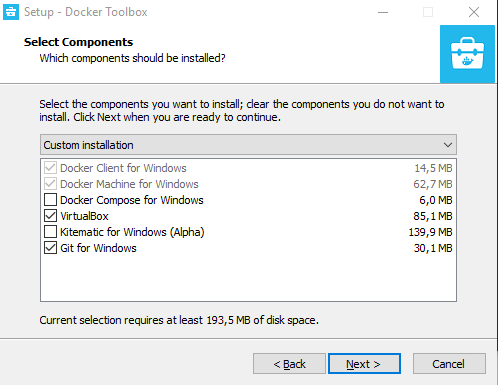
\includegraphics[width=0.45\textwidth]{\fig/DockerComponents.png}%
          \hspace{2ex}
          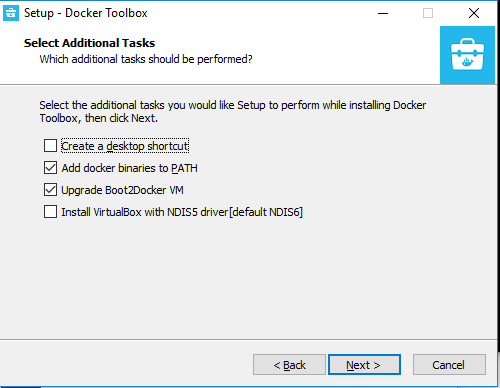
\includegraphics[width=0.45\textwidth]{\fig/DockerTasks.png}
          \caption{{\bf Left:} The minimal set of Docker components to select during the install.\\
                   {\bf Right:} Possible choice of additional Docker tasks.} 
          \label{fig:DockerComponents}
        \end{figure}
	After installation of the Docker Toolbox you need to run \verb'install.bat' (since system path variable was modified new shell is required). 
	\item Second step is customization of the Docker environment. The downloaded Flow123d image is imported into your docker environment 
	and further modified to provide better integration with your system.
	You will be asked several times to allow changes to the \emph{'VirtualBox Interface'}, do not hesitate to confirm any dialog containing 'Oracle'.
		
	Since flow123d run in the Docker container we must set a mapping of the Windows directories to the directories in the Docker container. 
	By default we setup such mapping for the home directory \verb'C:/Users' which is mapped to \verb'/c/Users'. 
	
	At the end of the second phase you are asked if you \dots \emph{'wish to add other mounts.'} Answering 'y' you can specify other disk for mapping 
	(recursively). The question is repeated allowing to add more custom mappings one by one. To mount other disks please enter only letter 
	of a disk you want to mount such as \verb'd'.
	If you agree to mount disk, virtual machine will be stopped 
	(this may take several seconds). Example of adding two disks can be following:
	\begin{verbatim}
		Do you wish to add other mounts? [y/N] y
		
		Stopping default to perform changes in virtual machine
		Enter letter of disk you want to mount (e.g. d): f
		Mounting path "f:" -> "/f/"
		Do you wish to add other mounts? [y/N] y
		
		Enter letter of disk you want to mount (e.g. d): g
		Mounting path "g:\" -> "/g/"
		Do you wish to add other mounts? [y/N] n
	\end{verbatim}
	
	\textbf{Note:}
	\textit{Mounting process does not copy or move any files. This process only grants permission to the virtual machine to work with files under mounted location.}
\end{enumerate}

In order to uninstall Flow123d you can run the \verb'uninstall.bat' script. This script removes Flow123d 
and uninstall Docker Toolbox (after confirmation), but keep Git and VirtualBox installed. These can be uninstalled manually. 
Moreover the configuration directories \verb'.docker' and \verb'VirtualBox' in your home directory are preserved. These can be deleted manually as well. 




\subsection{Reinstalling Flow123d}
\label{duplicit-image}
If you are installing same version of Flow123d again, you will be prompted whether to remove previous version or not. 
It is recommended to confirm deletion for both images \verb'flow123d/v<version>' and \verb'flow123d/v<version>:user'.


\section{Running Flow123d}

\subsection{Running Flow123d on Linux}
\label{subsec:running-flow123d-on-linux}
All necessary scripts for Flow123d are located in the \verb'bin' directory of installation directory \verb'Flow123d-<version>-linux-install'.
Docker container by default cannot easily interact with host file system. But using scripts in \verb'bin' will make things easier.
Directory \verb'bin' contains:
\begin{itemize}
	\item \verb'fterm.sh' \\
	 Script will invoke shell inside docker container and mount your home directory.
	 In this shell you have access to system where Flow123d is installed. By default command \verb'flow123d' is in the \verb'PATH' variable.
	 
	\textbf{Note:} On some systems, shell's font is extremely small, you can change this behaviour by right-clicking on window bar and selecting 
	\verb'default' or (\verb'vychozi' in Czech) see \autoref{fig:TerminalFont}.
	 \begin{figure}
		 \center
		 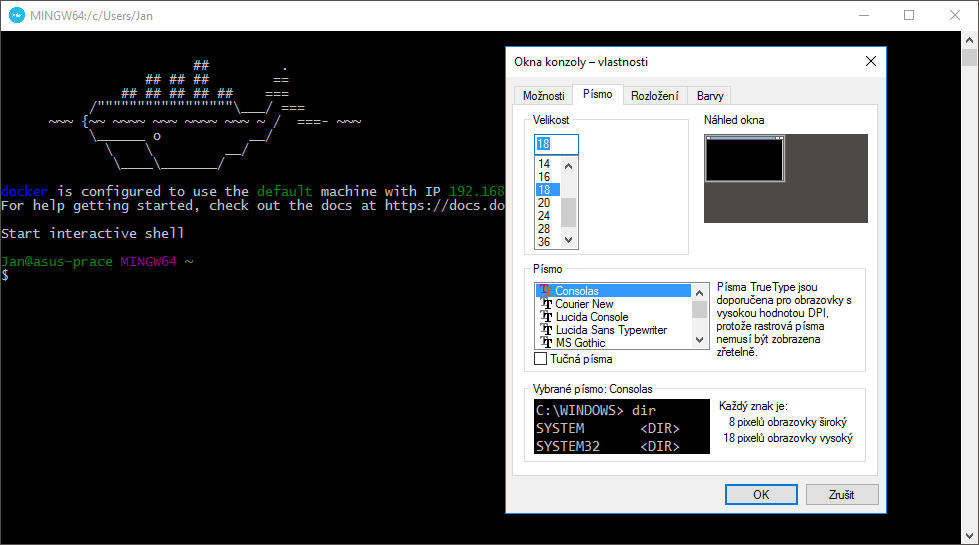
\includegraphics[width=1\textwidth]{\fig/TerminalFont.png}
		 \caption{Changing default font family and font size}
		 \label{fig:TerminalFont}
	 \end{figure}

	\item \verb'flow123d.sh' \\
	 Script will run Flow123d inside docker container and mount your home  directory.
	 All arguments passed to this script will be passed to \verb'flow123d' binary file inside docker.

	\item \verb'runtest.sh' \\
	 Script will run Flow123d tests inside docker container and mount your home  directory.
	 All arguments passed to this script will be passed to \verb'runtest.py' binary file inside docker.
	 
	\item \verb'configure' \\
	 Script is part of installation process and it modifies imported image for current active user. It will create user inside docker
	 with same name, user id and group id as current user.	 	 
\end{itemize}

\textbf{Note:}
\textit{Using above} \verb'.sh' \textit{scripts will mount your your home  directory to docker container under the same name.}
\textit{Also your current working directory will be the same. Example below shows behaviour of the scripts:}
\begin{verbatim}
$> pwd
/home/jan-hybs/install-folder

$> ls
bin  data  doc	install.sh  tests

$> bin/fterm.sh
Home directory mounted to '/home/jan-hybs'

jan-hybs@v2.0.0:/home/jan-hybs/install-folder$ ls
bin  data  doc	install.sh  tests
\end{verbatim}


\subsection{Running Flow123d on Windows}
On system Windows \verb'bat' files are located in the \verb'bin' directory of installation directory \verb'Flow123d-<version>-windows'.
Docker container by default cannot easily interact with host file system. But using scripts in \verb'bin' will make things easier.
Directory \verb'bin' contains two \verb'bat' files:
\begin{itemize}
	\item \verb'fterm.sh' see section \ref{subsec:running-flow123d-on-linux}
	
	\item \verb'fterm.bat' \\
	File serves as wrapper for script \verb'fterm.sh'. Executing this file will open up docker container shell.

	\item \verb'flow123d.sh' see section \ref{subsec:running-flow123d-on-linux}	
	
	\item \verb'flow123d.bat' \\
	File serves as wrapper for script \verb'flow123d.sh'. Executing this file will open up docker container shell and execute 
	Flow123d with given arguments. After execution \verb'bat' file exit itself. To see Flow123d output use file \verb'fterm.bat'
	and manually enter the command:
	\begin{verbatim}
		> fterm.bat
		me@v2.0.0 $ flow123d --help
	\end{verbatim}

	\item \verb'runtest.sh' see section \ref{subsec:running-flow123d-on-linux}	
	
	\item \verb'runtest.bat' \\
	File serves as wrapper for script \verb'runtest.sh'. Executing this file will open up docker container shell and execute 
	runtest script with given arguments.
\end{itemize}

\textbf{Note:}
\textit{Docker Engine daemon has only limited access to your Windows file system. Docker Machine tries to auto-share your}
\verb'C:\Users' \textit{directory. Directories outside this directory will not be automatically mounted.} 

\subsubsection{Running from other batch file}
The Windows system calls the batch files in the different way then the binaries. In particular the colling batch file is not processed further after the child batch 
file is done. In order to do so ane have to use the \verb'CALL' command. This is especially necessary for various calibration tools. The correct calling batch file 
may look like:
\begin{verbatim}
    echo "Starting Flow123d ..."
    call flow123d.bat a_simulation.yaml 
    echo "... simulation done."
\end{verbatim}


\subsection{Setting memory of virtual machine}
The virtual machine (VM) used for running the Docker with Flow123d inside claims predefined portion of the RAM 
of the host system to be used as the RAM of the guest Docker system. Unfortunately the default size of this memory is
quite small, e.g. 1GB on a 4GB machine. About 500MB is taken by the Docker kernel leaving just 500MB for Flow123d.
This is may be enough just for the small problems with thousands of elements. In order to treat realistic problems one have to 
enlarge the RAM size of the guest system. This can be easily done as follows:

\subsection{Issues with Windows 10}
Beginning with Windows 10, Microsoft apply all updates incrementally including major upgrades. As the Virtual Box deals with very internals of the system
any such update may broke it. The solution is to install manually the latest available version of the VirtualBox. In the case of fresh installation 
one also can not use automatical installotion of the Virtual Box by the Flow123d installer. An up-to-date version of Virtual Box has to be installed followed by 
installation of the Flow123d.

In particular for the "Creator's update" update, version 1703, you have to install at least version 5.2 
of the VirtualBox. Yet, starting the virtual machine it ends up with error \verb'NtCreateFile(\Device\VBoxDrvStub) failed: Unknown Status -626 ...}'. The workaround is:
uninstall VirtualBox, {\bf reboot}, install VirtualBox 5.2.  

 
\begin{enumerate}
 \item Start \verb'Oracle VM VirtualBox' either by a shortcut on your desktop or through the start menu. 
 A medium size window appears with the list of existing virtual machines 
 on the left. The docker VM is named 'default'.
 \item Next step is to power off the VM \verb'default' if it is running. 
 Following the left Figure \ref{fig:vm_ram_setup}, use the right-click on the VM and select \verb'Close' (Zav\v r\' it) and 
 \verb'Power Off' (Vypnout). Confirm the turn off of the VM machine. 
 \item Final step is setting the size of RAM of the VM. Follow the right Figure \ref{fig:vm_ram_setup}. 
 Select the VM \verb'default', click on \verb'Settings' (Nastave\' i) and select \verb'System' in the left column.
 On the tab \verb'Motherboard' (Z\' akladn\' i deska) you find a slide to select the size of the RAM. You can select sizes  
 in the orange or even red range since the memory is only reserved not actually used, however setting it to close to the 
 whole RAM size of the host allows the applications, i.e. Flow123d, running on the VM to compete for RAM with applications on the host system.
 \item The VM is restarted automatically at the next start of the Flow123d or the fterm.
\end{enumerate}


\begin{figure}
    \center  
    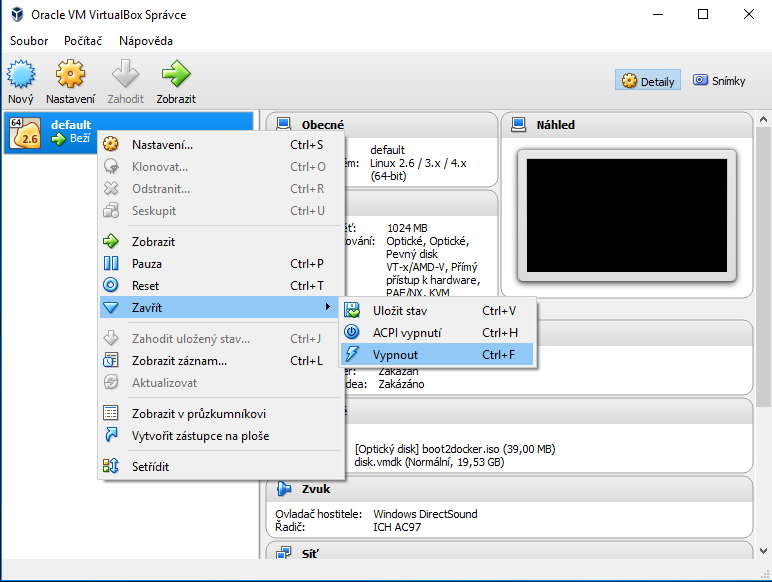
\includegraphics[width=0.45\textwidth]{\fig/VBMachineTurnOff.png}
    \hspace{2ex}
    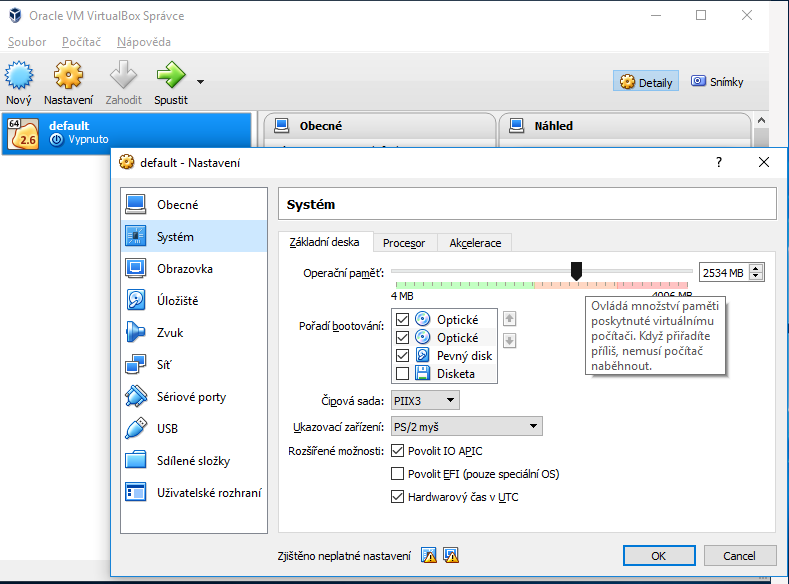
\includegraphics[width=0.45\textwidth]{\fig/VBMachineSetMem.png}
    \caption{{\bf Left:} Power off the virtual machine.
             {\bf Right:} Setting RAM size of the virtual machine.} 
    \label{fig:vm_ram_setup}
\end{figure}

\subsection{Flow123d arguments}
When you are inside docker container, you have access to entire file system. Flow123d is installed in 
\verb'/opt/flow123d' directory. Folder \verb'/bin' contains binary files and is automatically 
added to \verb'PATH' variable, meaning every executable in this folder can be called from anywhere.

Main Flow123d binary is located in \verb'bin/flow123d' and accepts following arguments:


\begin{description}
 \item[{\tt --help}] \hfill\\
        Help for parameters interpreted by Flow123d. Remaining parameters are passed to PETSC.
 \item[ {\tt -s, --solve} ] \verb'<file>' \hfill\\
 	 Set principal input file. Can be in YAML (or  JSON) file format. All relative paths of the input 
 	 files are relative to the location of the principal input file.
 \item[{\tt -i, --input\_dir}] \verb'<directory>' \hfill\\
 	The placeholder \verb"${INPUT}" %$
  	used in the path of an input file will be replaced by the \verb'<directory>'. Default value is \verb'input'.
 \item[{\tt -o, --output\_dir}] \verb'<directory>' \hfill\\
 	All paths for output files will be relative to this \verb'<directory>'. Default value is \verb'output'.
 \item[{\tt -l, --log}] \verb'<file_name>' \hfill\\
 	Set base name of log files. Default value is \verb'flow123d'. The log files are individual for every MPI process, placed in the output directory. 
 	The MPI rank of the process and the \verb'log' suffix are appended to the base name.
 \item[{\tt --no\_log}] \hfill\\
        Turn off logging.
 \item[{\tt --no\_profiler}] \hfill\\
        Turn off profiler output.
 \item[{\tt --petsc\_redirect <file>}] \hfill\\
        Redirect all PETSc stdout and stderr to given file.       
 \item[{\tt --input\_format}] \hfill\\ 
        Prints a description of the main input file in JSON format. Is used by GeoMop model editor and by python scripts for 
        generating reference documentation in Latex or HTML format.
 \item[{\tt --yaml\_balance}] \hfill\\
        Generate balance file also in machine readable YAML format. Will be default in future, used by GeoMop.
 \item[{\tt --no\_signal\_handler}] \hfill\\
        For debugging purpose.
        
\end{description}
All other parameters will be passed to the PETSC library. An advanced user can influence lot of parameters of linear solvers. In order to get list of supported options 
use parameter \verb'-help' together with some valid input. Options for various PETSC modules are displayed when the module is used for the first time.

Alternatively, you can use python script \verb'exec_parallel' located in \verb'bin/python' to start parallel jobs or limit resources used by the program.

After double dash specify which \verb'mpiexec' binary will be used (\verb'MPI-EXECUTABLE') and then specify what should be run. 
The script does not need to run solely \verb'flow123d'.

If we want to run command \verb'whoami' in parallel we can do:
\begin{verbatim}
	bin $> exec_parallel -n 4 -- ./mpiexec whoami
\end{verbatim}

To execute Flow123d in parallel we can do:
\begin{verbatim}
	bin $> exec_parallel -n 4 -- ./mpiexec ./flow123d --help
\end{verbatim}


\begin{verbatim}
  exec_parallel [OPTIONS] -- [MPI-EXECUTABLE] [PARAMS]
\end{verbatim}

The script has following options:

\begin{description}
  \item[{\tt -h, --help}] \hfill\\
  	Usage overview.
  \item[{\tt --host}] \verb'<hostname>' \hfill\\
  		Valid only when option \verb'--queue' is set.
        Default value is the host name obtained by python \verb'platform.node()' call, this argument can be used to override it. 
        Resulting value is used to select a correct PBS module from lookup table \verb'config/host_table.yaml'.
  \item[{\tt -n}] \verb'<number of processes>' \hfill\\
  	Specify number of MPI parallel processes for calculation.
  \item[{\tt -t, --limit-time}] \verb'<timeout>' \hfill\\
  	Upper estimate for real running time of the calculation. Kill calculation after {\it timeout} seconds. 
  	Value can also be \verb'float' number. When in PBS mode, value can also affect PBS queue. 
  \item[{\tt -m, --limit-memory}] \verb'<memory limit>' \hfill\\
  	Limits total available memory to \verb'<memory limit>' MB in total.
  \item[{\tt -q, --queue}] \verb'<queue>' \hfill\\
  		If set activates PBS mode. If argument \verb'queue' is also set selects particular job queue
  		on PBS systems otherwise default PBS queue is used. Default PBS queue automatically
  		choose valid queue based on resources.
\end{description}


Another script which runs Flow123d is \verb'runtest.sh'. This script will run tests specified as arguments. Script accepts both folders
and yaml files. To see full details run \verb'runtest.sh --help'. The script will run yaml tests and then compare results with reference
output. Example usage of the script:

\begin{verbatim}
$> bin/runtest.sh -n 1 tests/10_darcy/01_source.yaml 
...
Case 01 of 02
Running: 1 x 10_darcy/01_source
Done    | elapsed time 0:00:00:898                                              
    Comparison: 01 of 03 | 10_darcy: 01_source/flow.pvd (0.22kB)
    Comparison: 02 of 03 | 10_darcy: 01_source/flow/flow-000000.vtu (0.63MB)
    Comparison: 03 of 03 | 10_darcy: 01_source/water_balance.txt (0.32kB)
------------------------------------------------------------
Case 02 of 02
Running: 2 x 10_darcy/01_source
Done    | elapsed time 0:00:00:900                                              
    Comparison: 01 of 03 | 10_darcy: 01_source/flow.pvd (0.22kB)
    Comparison: 02 of 03 | 10_darcy: 01_source/flow/flow-000000.vtu (0.63MB)
    Comparison: 03 of 03 | 10_darcy: 01_source/water_balance.txt (0.32kB)
------------------------------------------------------------
Summary: 
    [ PASSED ]  | 1 x 10_darcy/01_source                        [ 1.40 sec] 
    [ PASSED ]  | 2 x 10_darcy/01_source                        [ 1.41 sec] 
    ------------------------------------------------------------
    [ PASSED ]  | passed=2, failed=0, skipped=0 in [ 2.81 sec]

\end{verbatim}





\section{Tutorial Problem}
\tbd{Update according new scheme or rather generate from commented YAML input file.}
In the following section, we shall provide an example cook book for preparing and running a model,
based on one of the test problems with the main input file:
\begin{verbatim}
tests/03_transport_small_12d/flow_vtk.con
\end{verbatim}
There is also a list of further tutorials which can be found in Chapter \ref{ch:tutorials}.
We shall start with preparation of the geometry using an external software and then we shall go thoroughly through the 
commented main input file. The problem includes steady Darcy flow, transport of two substances with explicit
time discretization and a reaction term consisting of dual porosity and sorption model.

\subsection{Geometry}
We consider a~simple 2D problem with a branching 1D fracture (see Figure \ref{fig:tutorial} for the geometry). 
To prepare a~mesh file we use the \href{http://geuz.org/gmsh/}{GMSH software}.
First, we construct a~geometry file. In our case the geometry consists of: 
\begin{itemize}
 \item one physical 2D domain corresponding to the whole square
 \item three 1D physical domains of the fracture
 \item four 1D boundary physical domains of the 2D domain
 \item three 0D boundary physical domains of the 1D domain
\end{itemize}
In this simple example, we can in fact combine physical domains in every group, however we use this more complex setting for
demonstration purposes. Using GMSH graphical interface we can prepare the GEO file where physical domains are referenced by numbers, then we use 
any text editor and replace numbers with string labels in such a way that the labels of boundary physical domains start with the dot character. 
These are the domains where we will not do any calculations but we will use them for setting boundary conditions.
Finally, we get the GEO file like this:

\begin{multicols}{2}
{\small
\begin{Verbatim}[numbers=left]
cl1 = 0.16;
Point(1) = {0, 1, 0, cl1};
Point(2) = {1, 1, 0, cl1};
Point(3) = {1, 0, 0, cl1};
Point(4) = {0, 0, 0, cl1};
Point(6) = {0.25, -0, 0, cl1};
Point(7) = {0, 0.25, 0, cl1};
Point(8) = {0.5, 0.5, -0, cl1};
Point(9) = {0.75, 1, 0, cl1};
Line(19) = {9, 8};
Line(20) = {7, 8};
Line(21) = {8, 6};
Line(22) = {2, 3};
Line(23) = {2, 9};
Line(24) = {9, 1};
Line(25) = {1, 7};
Line(26) = {7, 4};
Line(27) = {4, 6};
Line(28) = {6, 3};
\end{Verbatim}
\columnbreak
\begin{Verbatim}[numbers=left, firstnumber=last]
Line Loop(30) = {20, -19, 24, 25};
Plane Surface(30) = {30};
Line Loop(32) = {23, 19, 21, 28, -22};
Plane Surface(32) = {32};
Line Loop(34) = {26, 27, -21, -20};
Plane Surface(34) = {34};
Physical Point(".1d_top") = {9};
Physical Point(".1d_left") = {7};
Physical Point(".1d_bottom") = {6};
Physical Line("1d_upper") = {19};
Physical Line("1d_lower") = {21};
Physical Line("1d_left_branch") = {20};
Physical Line(".2d_top") = {23, 24};
Physical Line(".2d_right") = {22};
Physical Line(".2d_bottom") = {27, 28};
Physical Line(".2d_left") = {25, 26};
Physical Surface("2d") = {30, 32, 34};
\end{Verbatim}
}
\end{multicols}

Notice the labeled physical domains on lines 26 -- 36. Then we just set the discretization step \verb'cl1' and use GMSH to create the mesh file.
The mesh file contains both the 'bulk' elements where we perform calculations and the 'boundary' elements (on the boundary physical domains) where we only set the boundary conditions.

\subsection{CON File Format}
The main input file uses a slightly extended JSON file format which together with some particular constructs forms a CON (C++ object notation) file format. 
Main extensions of the JSON are unquoted key names (as long as they do not contain whitespaces), possibility to use \verb'=' instead of \verb':' 
and C++ comments, i.e. \verb'//' for a one line and \verb'/* */' for a multi-line comment. In CON file format, we prefer to call JSON objects ``records'' and we introduce also ``abstract records''
that mimic C++ abstract classes, arrays of a CON file have only elements of the same type (possibly using abstract record types for polymorphism). 
The usual keys are in lower case and without spaces (using underscores instead),
there are few special upper case keys that are interpreted by the reader: \verb'REF' key for references, \verb'TYPE' key for specifing actual type of an abstract record.
For detailed description see Section \ref{sec:CONformat}.


Having the computational mesh from the previous step, we can create the main input file with the description of our problem. 
\begin{Verbatim}[numbers=left]
{
  problem = {
    TYPE = "SequentialCoupling", 
    description = "Tutorial problem: 
    Transport 1D-2D (convection, dual porosity, sorption, sources).", 
    mesh = {
      mesh_file = "./input/mesh_with_boundary.msh",
      sets = [
          { name="1d_domain", 
            region_labels = [ "1d_upper", "1d_lower", "1d_left_branch" ]
          }
        ]
    }, // mesh
\end{Verbatim}
The file starts with a selection of problem type (\verb'SequentialCoupling'), and a textual problem description.
Next, we specify the computational mesh, here it consists of the name of the mesh file and the declaration of one {\it region set} 
composed of all 1D regions i.e. representing the whole fracture. Other keys of the \Alink{IT::Mesh}{\tt mesh} record allow labeling regions given only by numbers, 
defining new regions in terms of element numbers (e.g to have leakage on single element), 
defining boundary regions, and set operations with region sets, see Section \ref{sec:Mesh} for details.

\subsection{Flow Setting}
Next, we setup the flow problem. We shall consider a flow driven only by the pressure gradient (no gravity),
setting the Dirichlet boundary condition on the whole boundary with the pressure head equal to $x+y$. 
The \Alink{Flow-Darcy-MH-Data::conductivity}{\tt conductivity} will be $k_2=10^{-7}$ \unitss{}{1}{-1} on the 2D domain and $k_1=10^{-6}$ \unitss{}{1}{-1} on the 1D domain.
Both 2D domain and 1D domain \Alink{Flow-Darcy-MH-Data::cross-section}{\tt cross\_section} will be set by default,
meaning that the thickness of 2D domain is $\delta_2=1$ \unitss{}{1}{} and the fracture cross section is $\delta_1=1$ \unitss{}{2}{}.
The transition coefficient $\sigma_2$ between dimensions can be scaled by setting the dimensionless parameter 
$\sigma_{21}$ (\Alink{Flow-Darcy-MH-Data::sigma}{\tt sigma}). This can be used for simulating additional
effects which prevent the liquid transition from/to a fracture, like a thin resistance layer. Read Section 
\ref{sec:darcy_flow} for more details.

\begin{Verbatim}[numbers=left, firstnumber=last]
    primary_equation = {
      TYPE = "Steady_MH", 

      input_fields = [
        { r_set = "1d_domain", conductivity = 1e-6, 
                               cross_section = 0.04, 
                               sigma = 0.9 },
        { region = "2d",       conductivity = 1e-7  },
        { r_set = "BOUNDARY",
          bc_type = "dirichlet",
          bc_pressure = { TYPE="FieldFormula", value = "x+y" }
        }
      ],

     output = {
        output_stream = { 
          file = "flow.pvd", 
          format = { TYPE = "vtk", variant = "ascii" }
        }, 
        output_fields = [ "pressure_p0", "pressure_p1", "velocity_p0" ]
      }, 
      
      solver = {
        TYPE = "Petsc",
        a_tol = 1e-12,
        r_tol = 1e-12
      }
    }, // primary equation
\end{Verbatim}
On line 15, we specify particular implementation (numerical method) of the flow solver, in this case the Mixed-Hybrid
solver for steady problems. On lines 17 -- 24, we set both mathematical fields that live on the computational domain 
and those defining the boundary conditions. We set only the conductivity field since other \hyperA{IT::Flow-Darcy-MH-Data}{\tt input\_fields} have appropriate default values.
We use implicitly defined set ``BOUNDARY'' that contains all boundary regions and set there dirichlet boundary condition in terms of the 
pressure head. In this case, the field is not of the implicit type {\tt FieldConstant}, so we must specify the type of the field {\tt TYPE="FieldFormula"}.
See Section \ref{sec:Fields} for other field types. 
On lines 26 -- 32, we specify which output fields should be written to the output stream (that means particular output file, with given format).
Currently, we support only one output stream per equation, so this allows at least switching individual output fields on or off. 
See Section \ref{section_output} for the list of available \Alink{IT::Flow-Darcy-MH-output-fields}{\tt output\_fields}.
Finally, we specify type of the linear solver and its tolerances.



\subsection{Transport Setting}
The flow model is followed by a transport model in the \Alink{Coupling-Sequential::solute-equation}{\tt solute\_equation}
beginning on line 40. For the transport problem, we use an implementation called \hyperA{IT::Solute-Advection-FV}{Solute\_Advection\_FV}
which stands for an explicit finite volume solver of the convection equation (without diffusion).
The operator splitting method is used for equilibrium sorption as well as for dual porosity model and 
first order reactions simulation.

\begin{Verbatim}[numbers=left, firstnumber=last]
    secondary_equation = {
      TYPE = "Solute-Advection-FV", 

      substances = [ 
        {name = "age", molar_mass = 0.018},     // water age
        {name = "U235", molar_mass = 0.235}     // uranium 235
      ],
      
      input_fields= [
        { r_set = "ALL",
          init_conc = 0,
          porosity= 0.25,
          sources_density = [1.0, 0]
        },
        { r_set = "BOUNDARY",
          bc_conc = [0.0, 1.0]
        }
      ],
      
      time = { end_time = 1e6 },
      mass_balance = { cumulative = true },
\end{Verbatim}

On lines 43 -- 46, we set the transported \Alink{Coupling-OperatorSplitting::substances}{\tt substances}, 
which are identified by their names. Here, the first one is the \verb'age' of the water, with the molar mass of water, 
and the second one \verb'U235' is the uranium isotope 235. 
On lines 48 -- 57, we set the input fields, in particular zero initial concentration for all substances,
\Alink{Solute-Advection-FV-Data::porosity}{\tt porosity} $\theta = 0.25$ and 
sources of concentration by \Alink{Solute-Advection-FV-Data::sources-density}{\tt sources\_density}. 
Notice line 50 where we can see only single value since an automatic conversion is applied to turn the scalar 
zero into the zero vector (of size 2 according to the number of substances). 

The boundary fields are set on lines 54 -- 56. We need not to specify the type of the condition since there is 
only one type in the current transport model. The boundary condition is equal to $1$ for the uranium 235 and $0$ 
for the age of the water and is automatically applied only on the inflow part of the boundary. 

We also have to prescribe the \hyperA{IT::TimeGovernor}{\tt time} setting, here only the end time of the simulation
(in seconds: $10^6\,\rm{s}\approx 11.57$ days) is required since the step size is determined from the CFL condition. 
However, a smaller time step can be enforced if necessary.

Reaction term of the transport model is described in the next subsection, including dual porosity and sorption.

\subsection{Reaction Term}\label{subsubsec:reactions}
The input information for dual porosity, equilibrial sorption and possibly first order reations are enclosed in the record 
\Alink{Coupling-OperatorSplitting::reaction-term}{\tt reaction\_term}, lines 61 -- 100. Go to section \ref{sec:reaction_term}
to see how the models can be chained.

The type of the first process is determined by {\tt TYPE="DualPorosity"}, on line 62. 
The \Alink{DualPorosity::input-fields}{\tt input\_fields}
of dual porosity model are set on lines 64 -- 71 and the output is disabled by setting an empty array on line 73.

\begin{Verbatim}[numbers=left, firstnumber=last]
      reaction_term = {
        TYPE = "DualPorosity",
        
        input_fields= [
          {
            r_set="ALL",
            diffusion_rate_immobile = [0.01,0.01],
            porosity_immobile = 0.25,
            init_conc_immobile = [0.0, 0.0]
          }
        ],
        
        output_fields = [],
        
        reaction_mobile = {
          TYPE = "SorptionMobile",
          solvent_density = 1000.0,     // water
          substances = ["age", "U235"],
          solubility = [1.0, 1.0],
          
          input_fields= [
            {
              r_set="ALL",
              rock_density = 2800.0,    // granit
              sorption_type =  ["none", "freundlich"],
              isotherm_mult = [0, 0.68], 
              isotherm_other = [0, 1.0]
            }
          ],
          output_fields = []
        },
        reaction_immobile = {
          TYPE = "SorptionImmobile",
          solvent_density = 1000.0,     // water
          substances = ["age", "U235"],
          solubility = [1.0, 1.0],
          input_fields = { REF="../../reaction_mobile/input_fields" },
          output_fields = []
        }
      },
      
      output_stream = { 
        file = "transport.pvd", 
        format = { TYPE = "vtk", variant = "ascii" },
        time_step = 1e5      
      } 

    } // secondary_equation
  } // problem
}
\end{Verbatim}

Next, we define the equilibrial sorption model such that \hyperA{IT::SorptionMobile}{\tt SorptionMobile} type takes place in the mobile 
zone of the dual porosity model while \hyperA{IT::SorptionImmobile}{\tt SorptionImmobile} type takes place in its immobile zone, see lines 76 and 93.
Isothermally described sorption simulation can be used in the case of low concentrated solutions without competition between multiple dissolved species.

On lines 77 -- 89, we set the sorption related input information. The solvent is water so the \Alink{Sorption::solvent-density}{\tt solvent\_density} 
is supposed to be constant all over the simulated area. The vector \Alink{Sorption::substances}{\tt substances} 
contains the list of names of soluted substances which are considered to be affected by the sorption.
Solubility is a material characteristic of a sorbing substance related to the solvent. Elements of the vector 
\Alink{Sorption::solubility}{\tt solubility} define the upper bound of aqueous concentration which can appear.
This constrain is necessary because some substances might have limited solubility and if the solubility exceeds 
its limit they start to precipitate. {\tt solubility} is a crucial parameter for solving a set of nonlinear 
equations, described further. 

The record \hyperA{IT::Sorption-Data}{\tt input\_fields} covers the region specific parameters.
All implemented types of sorption can take the rock density in the region into account. The value of 
\Alink{Sorption-Data::rock-density}{\tt rock\_density} is a constant in our case. 
The \Alink{Sorption-Data::sorption-type}{\tt sorption\_type} represents the empirically determined isotherm 
type and can have one of four possible values: \{{\tt"none"}, {\tt"linear"}, {\tt"freundlich"}, {\tt"langmuir"}\}. 
Linear isotherm needs just one parameter given whereas Freundlichs' and Langmuirs' isotherms require two parameters. 
We will use Freundlich's isotherm for demonstration but we will set the other parameter (exponent) $\alpha=1$ 
which means it will be the same as the linear type. 

Let suppose we have a sorption coefficient for uranium $K_d=1.6\cdot10^{-4}$ \unitss{-1}{3}{} (www.skb.se, report R-10-48 by James Crawford, 2010) 
and we want to use. We need to convert it to dimensionless value of \Alink{Sorption-Data::isotherm-mult}{\tt isotherm\_mult}
in the following way: $k_l = K_dM_s^{-1}\rho_l = K_d\frac{1000}{0.235}\approx0.68$. For further details, see 
mathematical description in Section \ref{sec:sorp_math}. 

On line 97, notice the reference pointing to the definition of input fields on lines 81 -- 89. Only entire records 
can be referenced which is why we have to repeat parts of the input such as solvent density and solubility 
(records for reaction mobile and reaction immobile have different types).

On lines 90 and 98, we define which sorption specific outputs are to be written to the output file. 
An implicit set of outputs exists. In this case we define an empty set of outputs thus overriding the implicit one. 
This means that no sorption specific outputs will be written to the output file.
On lines 102 -- 106 we specify which output fields should be written to the output stream. Currently, we support output into VTK and GMSH data format.
In the output record for time-dependent process we have to specify the {\tt time\_step} (line 105) which determines the frequency of saving.



\subsection{Results}
In Figure \ref{fig:tutorial} one can see the results: the pressure and the velocity field on the left and the 
concentration of U235 at time $t=9\cdot10^{5}$ s on the right. Even if the pressure gradient is the same in the 
2D domain and in the fracture, due to higher conductivity the velocity field is ten times faster in the fracture. 
Since porosity is the same, the substance is transported faster by the fracture and then appears in the bottom 
left 2D domain before the main wave propagating solely through the 2D domain.

% The output files can be either \verb'*.msh' files accepted by the GMSH or one can use VTK format that can be post-processed by Paraview.


\begin{figure}[ht]
    \centering
    \begin{subfigure}[b]{0.48\textwidth}
        \centering
        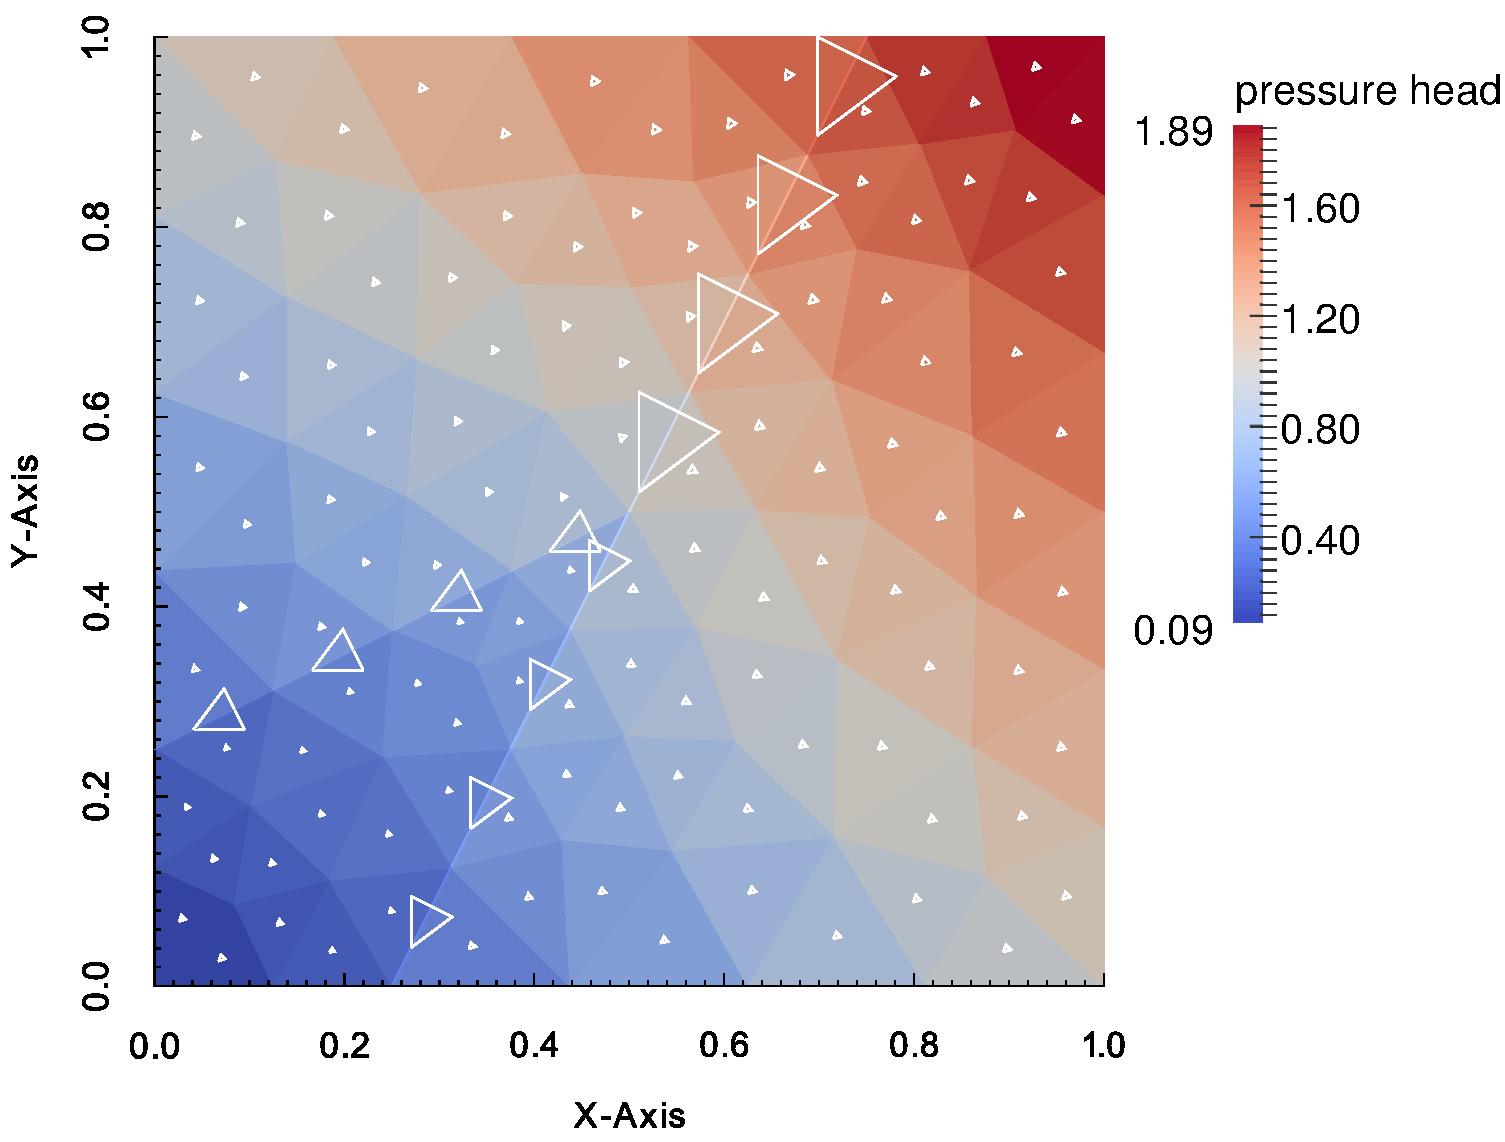
\includegraphics[width=\textwidth]{\fig/03_flow.pdf}
        % 03_flow.pdf: no raster
        \caption{Elementwise pressure head and\\velocity field denoted by triangles.\\ (Steady flow.)}
        \label{fig:tut-flow}
    \end{subfigure}
    ~
    \begin{subfigure}[b]{0.48\textwidth}
        \centering
        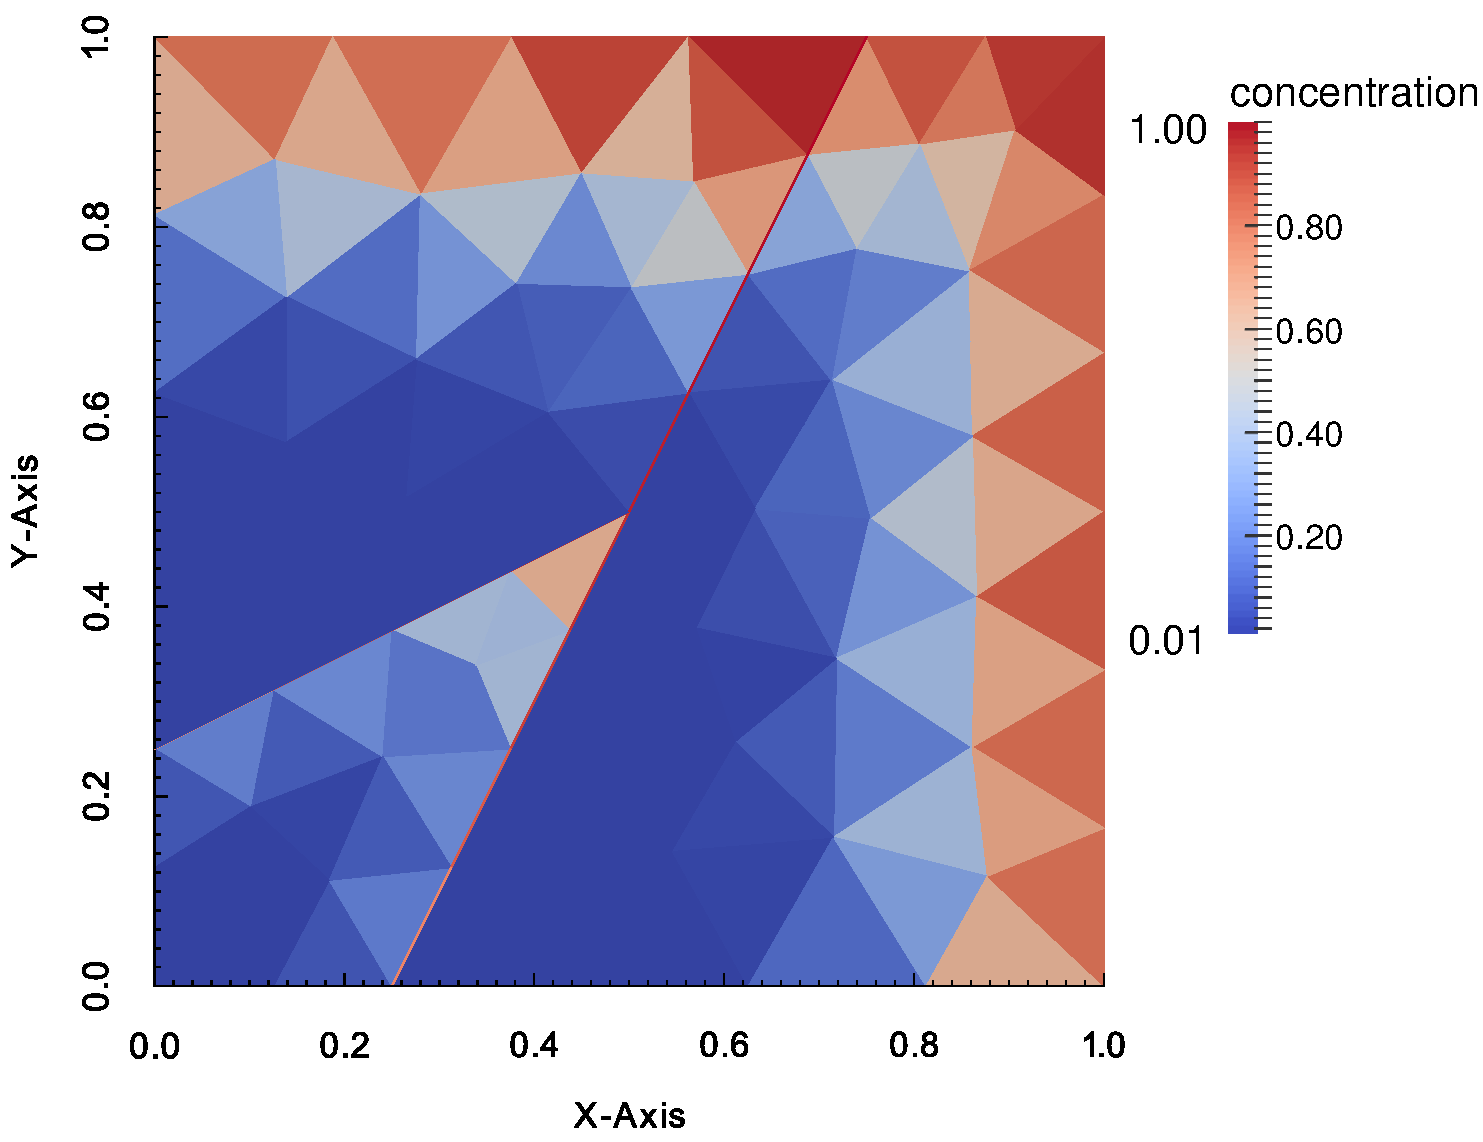
\includegraphics[width=\textwidth]{\fig/03_trans.pdf}
        % 03_trans.pdf: no raster
        \caption{Propagation of U235 from the inflow part of the boundary. \\ (At the time $9\cdot10^{5}$ s.)}
        \label{fig:tut-trans}
    \end{subfigure}
    \caption{Results of the tutorial problem.}
    \label{fig:tutorial}
\end{figure}







\chapter[Mathematical Models of Physical Reality]{Mathematical Models \\of Physical Reality}
\label{chapter:mathematical_models}

In this chapter we describe mathematical models used in Flow123d.
Then in chapter \ref{chapter:file-formats} we briefly describe structure of individual input files, in particular the main YAML file.
The complete description of the YAML format is given in chapter \ref{chapter:input-tree-reference}.

Flow123d provides models for Darcy flow in porous media as well as for the transport and reactions of solutes. In this section, we describe 
mathematical formulations of these models together with physical meaning and units of all involved quantities. In the first section we present 
basic notation and assumptions about computational domains and meshes that combine different dimensions. In the next section we
derive approximation of thin fractures by lower dimensional interfaces for a general transport process. Latter sections describe details for models of particular
physical processes.

\section{Meshes of Mixed Dimension}
Unique feature common to all models in Flow123d is the support of
domains with mixed dimension. 
Let $\Omega_{3} \subset \Real^3$ be an open set representing continuous approximation of porous and fractured medium.
Similarly, we consider a set of 2D manifolds $\Omega_2\subset\overline\Omega_3$, representing the 2D fractures and a set of 1D manifolds $\Omega_1\subset \overline\Omega_2$ 
representing the 1D channels or preferential paths (see Fig \ref{fig:multi-dim}).
We assume that $\Omega_2$ and $\Omega_1$ are polytopic (i.e. polygonal and piecewise linear, respectively).
For every dimension $d=1,2,3$, we introduce a triangulation $\mathcal{T}_{d}$ of the open set $\Omega_d$
that consists of finite elements $T_{d}^{i},$\ $i = 1,\dots,N_{E}^{d}$.
The elements are simplices, i.e. lines, triangles and tetrahedra, respectively.

\begin{figure}[h]
\centering
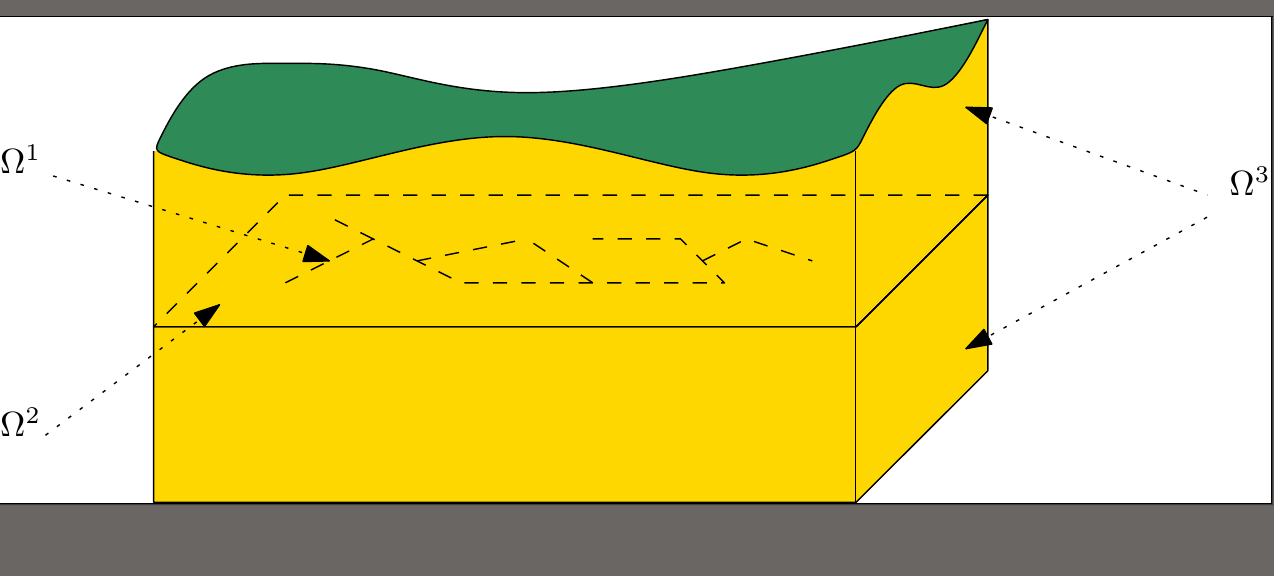
\includegraphics[width=10cm]{\fig/ground_fractures}
\caption{
    \label{fig:multi-dim}
    Scheme of a problem with domains of multiple dimensions.
}
\end{figure}

Present numerical methods used by the software require meshes satisfying the compatibility conditions
\begin{equation}
        T_{d-1}^i \cap T_d \subset \mathcal{F}_d,   \qquad \text{where } \mathcal{F}_d = \bigcup_{k} \partial T_{d}^{k}
\end{equation}
and
\begin{equation}
        T_{d-1}^i \cap \mathcal{F}_d    \text{ is either $T_{d-1}^i$ or $\emptyset$}    
\end{equation}
for every $i\in\{1,\dots, N_{E}^{d-1}\}$, $j\in\{1,\dots,N_{E}^{d}\}$,  and $d=2,3$. 
That is, the $(d-1)$-dimensional elements are either between $d$-dimensional elements and
match their sides or they poke out of $\Omega_d$. Support for a coupling between non-compatible
meshes of different dimesion is in developement and partly supported by the Darcy Flow model.

\section{Advection-Diffusion Processes on Fractures}
\label{sc:ad_on_fractures}
This section presents derivation of an abstract advection-diffusion process on 2D and 1D manifolds and its coupling with
the higher dimensional domains. The reader not interested in the details of this approximation may skip directly to
the later sections describing mathematical models of individual physical processes.

As was already mentioned, the unique feature of Flow123d is support of models living on 2D and 1D manifolds. The aim is to capture 
features significantly influencing the solution despite of their small cross-section. Such a tiny features are
challenging for numerical simulations since a direct discretization requires highly refined
computational mesh. One possible solution is to model these features (fractures, channels) 
as lower dimensional objects (2D and 1D manifolds) and introduce their coupling with the surrounding continuum.
The equations modeling a physical process on a manifold as well as its coupling to the model in the surrounding continuum
has to be derived from the model on the 3D continuum. This section presents such a procedure for the case of the abstract
advection-diffusion process inspired by the paper \cite{martin_modeling_2005}. Later, we this abstract approach to 
particular advection-diffusion processes: Darcian flow, solute transport, and heat transfer.

Let us consider a fracture as a strip domain 
\[
 \Omega_f \subset [0,\delta] \times \Real^{d-1}
\]
for $d=2$ or $d=3$ and surrounding continuum domains
\[
 \Omega_1 \subset (-\infty,0)\times \Real^{d-1},
 \Omega_2 \subset (\delta,\infty)\times \Real^{d-1}.
\]
Further, we denote by $\gamma_i$, $i=1,2$ the fracture faces common with domains $\Omega_1$ and $\Omega_2$ respectively.
By $x$, $\vc y$ we denote normal and tangential coordinate of a point in $\Omega_f$. 
We consider the normal vector  $\vc n=\vc n_1=-\vc n_2=(1,0,0)^\top$.
An advection-diffusion process is given by equations:
\begin{align}
  \label{eq:fr:continuity}
  \prtl_t w_i + \div \vc j_i &= f_i&&  \text{on } \Omega_i,\ i=1,2,f,\\
  \label{eq:fr:flux}
  \vc j_i &= - \tn A_i\grad u_i + \vc b_i w_i&& \text{on } \Omega_i,\ i=1,2,f,\\
  \label{eq:fr:Dirichlet}
  u_i &= u_f&& \text{on } \gamma_i,\ i=1,2,\\
  \label{eq:fr:Neumann}
  \vc j_i \cdot \vc n &= \vc j_f \cdot \vc n&& \text{on } \gamma_i,\ i=1,2,
\end{align}
where $w_i=w_i(u_i)$ is the conservative quantity and $u_i$ is the principal unknown, $\vc j_i$ is the flux of $w_i$, $f_i$ is the source term,
$\tn A_i$ is the diffusivity tensor and $\vc b_i$ is the velocity field. We assume that the tensor $\tn A_f$ is symmetric positive definite 
with one eigenvector in the direction $\vc n$. Consequently the tensor has the form:
\[
 A_f = \begin{pmatrix} 
            a_n & 0  \\
            0 & \tn A_t
       \end{pmatrix}
\]
Furthermore, we assume that $\tn A_f(x, \vc y)=\tn A_f(\vc y)$ is constant in the normal direction.

Our next aim is to integrate equations on the fracture $\Omega_f$ in the normal direction 
and obtain their approximations on the surface $\gamma=\Omega_f \cap \{x=\delta/2\}$ running through the middle of the fracture. 
For the sake of clarity, we will not write subscript $f$ for quantities on the fracture. 
To make the following procedure mathematicaly correct we have to assume that functions
$\prtl_x w$, $\prtl_x \grad_{\vc y} u$, $\prtl_x \vc b_{\vc y}$ are continuous and bounded on $\Omega_f$. Here and later on 
$\vc b_x=(\vc b \cdot \vc n)\, \vc n$ is the normal part of the velocity field and $\vc b_{\vc y} = \vc b - \vc b_x$ is the tangential part.
The same notation will be used for normal and tangential part of the field $\vc q$.

We integrate \eqref{eq:fr:continuity} over the fracture opening $[0,\delta]$ and use approximations to get
\begin{equation}
    \label{eq:fracture_continuity}
   \prtl_t (\delta W) - \vc j_2 \cdot \vc n_2 - \vc j_1 \cdot \vc n_1 + \div \vc J = \delta F,
\end{equation}
where for the first term, we have used mean value theorem, first order Taylor expansion, 
and boundedness of $\prtl_x w$ to obtain approximation:
\[
    \int_0^\delta w(x,\vc y) \d x=\delta w(\xi_{\vc y}, \vc y) = \delta W(\vc y) + O(\delta^2\abs{\prtl_x w}),
\]
where
\[
    W(\vc y)=w(\delta / 2,\vc y)=w(u(\delta/2,\vc y))=w(U(\vc y)).
\]
Next two terms in \eqref{eq:fracture_continuity} come from the exact integration 
of the divergence of the normal flux $\vc j_x$.
Integration of the divergence of the tangential flux $\vc j_{\vc y}$ gives the fourth term, where we introduced
\[
\vc J(\vc y) = \int_0^\delta \vc j_{\vc y}(x, \vc y) \d x.
\]
In fact, this flux on $\gamma$ is scalar for the case $d=2$. Finally, we integrate the right-hand side to get 
\[
    \int_0^\delta f(x,\vc y) \d x = \delta F(\vc y) + O(\delta^2\abs{\prtl_x f}),\quad F(\vc y)=f(\delta/2,\vc y). 
\]


Due to the particular form of the tensor $\tn A_f$, we can separately integrate tangential and normal
part of the flux given by \eqref{eq:fr:flux}. Integrating the tangential part and using approximations
\[
    \int_0^\delta  \grad_{\vc y} u(x, \vc y) \d x = \delta \grad_{\vc y} u (\xi_{\vc y}, \vc y) 
    = \delta \grad_{\vc y} U( \vc y) + O\big( \delta^2 \abs{\prtl_x\grad_{\vc y} u} \big) 
\]
and
\[
 \int_0^\delta \big(\vc b_{\vc y} w\big)(x, \vc y) \d x 
  = \delta \vc B(\vc y) W(\vc y) + O\big(\delta^2 \abs{\prtl_x(\vc b_{\vc y} w)} \big)
\]
where
\[
  \vc B(\vc y) = \vc b_{\vc y}(\delta/2, \vc y),
\]
we obtain
\begin{equation}
    \label{eq:fracture_darcy}
   \vc J = -\tn A_t \delta \grad_{\vc y} U + \delta \vc B W + O\big(\delta^2(\abs{\prtl_x\grad_{\vc y} u}+\abs{\prtl_x(\vc b_{\vc y} w)})\big).
\end{equation}


So far, we have derived equations for the state quantities $U$ and $\vc J$ on the fracture manifold $\gamma$. In order to
get a well possed problem, we have to prescribe two conditions for boundaries $\gamma_i$, $i=1,2$. To this end, we
perform integration of the normal flux $\vc j_x$, given by \eqref{eq:fr:flux}, separately for the left and right half of the fracture.
Similarly as before we use approximations
\[
 \int_0^{\delta/2} \vc j_x \d x = (\vc j_1 \cdot \vc n_1)\frac{\delta}{2} + O(\delta^2 \abs{\prtl_x \vc j_x})
\]
and 
\[
 \int_0^{\delta/2} \vc b_x w \d x = (\vc b_1 \cdot \vc n_1)\tilde{w}_1\frac{\delta}{2} + O(\delta^2 \abs{\prtl_x \vc b_x}\abs{w} + \delta^2\abs{\vc b_x}\abs{\prtl_x w})
\]
and their counter parts on the interval $(\delta/2, \delta)$ to get
\begin{align}
    \label{eq:fracture_normal_1}
     \vc j_1 \cdot \vc n_1 &= -\frac{2a_n}{\delta} (U - u_1) + \vc b_1\cdot \vc n_1 \tilde{w}_1\\
    \label{eq:fracture_normal_2}
    \vc j_2 \cdot \vc n_2 &= -\frac{2a_n}{\delta} (U - u_2) + \vc b_2\cdot \vc n_2 \tilde{w}_2
\end{align}
where $\tilde w_i$ can be any convex combination of $w_i$ and $W$. Equations \eqref{eq:fracture_normal_1}  
and \eqref{eq:fracture_normal_2} have meaning of a semi-discretized flux from domains $\Omega_i$ into fracture.
In order to get a stable numerical scheme, we introduce a kind of upwind already on this level using a different convex 
combination for each flow direction:
\begin{align}
   \notag 
   \vc j_i \cdot \vc n_i
       = &-\sigma_i (U - u_i)      \\ 
   \notag
      &+ \big[\vc b_i\cdot \vc n_i\big]^{+} \big(\xi w_i + (1-\xi) W\big)       \\
      \label{eq:fracture_normal}
      &+ \big[\vc b_i\cdot \vc n_i\big]^{-} \big((1-\xi) w_i + \xi W\big), \qquad i=1,2
\end{align}
where $\sigma_i = \frac{2a_n}{\delta}$ is the transition coefficient and the parameter $\xi\in [\frac12, 1]$ can be used to interpolate
between upwind ($\xi = 1$) and central difference ($\xi=\frac12$) scheme. Equations \eqref{eq:fracture_continuity}, \eqref{eq:fracture_darcy}, and
\eqref{eq:fracture_normal} describe the general form of the advection-diffusion process on the fracture and its communication with 
the surrounding continuum which we shall later apply to individual processes.



\section{Darcy Flow Model} \label{sec:darcy_flow}
We consider the simplest model for the velocity of the steady or unsteady flow in porous and fractured medium given by 
the Darcy flow:
\begin{equation}
    \label{eq:darcy}
    \vc w = -\tn K \grad H \quad\text{in }\Omega_d,\ \text{for $d=1,2,3$}.
\end{equation}
Here and later on, we drop the dimension index $d$ of the quantities if it can be deduced from the context.
In \eqref{eq:darcy}, $\vc w$ \units{}{1}{-1} is \href{http://en.wikipedia.org/wiki/Superficial_velocity}{the superficial velocity},
$\tn K_d$ is the conductivity tensor, and $H$ \units{}{1}{} is the piezometric head. The velocity $\vc w_d$ is related to the flux $\vc q_d$ 
\units{}{4-d}{-1} through
\[
    \vc q_d = \delta_d \vc w_d,
\]
where $\delta_d$ \units{}{3-d}{} is the \hyperA{Flow-Darcy-MH-Data::cross-section}{cross section} coefficient,
in particular $\delta_3=1$, $\delta_2$ \units{}{1}{} is the thickness of a~fracture, and $\delta_1$ \units{}{2}{} is the cross-section of a~channel.
The flux $\vc q_d\cdot\vc n$ is the volume of the liquid (water) that passes through a~unit square ($d=3$),
unit line ($d=2$), or through a~point ($d=1$) per one second. 
The conductivity tensor is given by the product \penalty-500
$\tn K_d = k_d \tn A_d$, where $k_d>0$ \units{}{1}{-1}
 is the \hyperA{Flow-Darcy-MH-Data::conductivity}{hydraulic conductivity}  and 
$\tn A_d$  is the 
$3\times 3$ dimensionless \hyperA{Flow-Darcy-MH-Data::anisotropy}{anisotropy tensor} which has to be symmetric and positive definite.
The piezometric-head $H_d$ is related to the pressure head
$h_d$ through
\begin{equation}
    \label{eq:piezo_head}
    H_d = h_d + z
\end{equation}
assuming that the gravity force acts in the negative direction of the $z$-axis. 
Combining these relations, we get the Darcy law in the form:
\begin{equation}
    \label{eq:darcy_flux}
    \vc q = -\delta k\tn A \grad (h+z)  \qquad\text{in }\Omega_d,\ \text{for $d=1,2,3$}.
\end{equation}

Next, we employ the continuity equation for saturated porous medium and the dimensional reduction from the preceding section
(with $w=u:=H$, $\vc j:=\vc w$, $\tn A:=\tn K$ and $\vc b:=\vc 0$), which yields:
\begin{equation}
    \label{eq:continuity}
    \prtl_t (\delta S\, h) + \div \vc q = F \qquad \text{in }\Omega_d,\ \text{for $d=1,2,3$},
\end{equation}
where  $S_d$ \units{}{-1}{} is the \hyperA{Flow-Darcy-MH-Data::storativity}{storativity} and $F_d$ \units{}{3-d}{-1} is 
the source term. In our setting the principal unknowns of the system 
(\ref{eq:darcy_flux}, \ref{eq:continuity}) are the pressure head $h_d$ and the flux $\vc q_d$.


The storativity (or the volumetric specific storage) $S_d>0$ can be expressed as
\begin{equation}
  S_d = \gamma_w(\beta_r + \vartheta \beta_w),
\end{equation}
where $\gamma_w$ \units{1}{-2}{-2} is the specific weight of water, $\vartheta$ \units{}{}{} is the porosity,
$\beta_r$ is compressibility of the bulk material of the pores (rock)
and $\beta_w$ is compressibility of the water, both with units \units{-1}{1}{-2}. For steady problems, we set $S_d=0$ for all dimensions $d=1,2,3$.
The source term $F_d$ on the right hand side of \eqref{eq:continuity} consists of the volume density of the 
\hyperA{Flow-Darcy-MH-Data::water-source-density}{water source} 
 $f_d$\units{}{}{-1} and flux from the from the higher dimension. 
Precise form of $F_d$ slightly differs for every dimension and will be discussed presently.

In $\Omega_3$ we simply have $F_3  = f_3$ \units{}{}{-1}.

\subsection{Coupling on mixed meshes}
In the set $\Omega_2 \cap \Omega_3$ the fracture is surrounded by at most one 3D surface from every side.
On $\prtl\Omega_3 \cap \Omega_2$ we prescribe a~boundary condition of the Robin type:
\begin{align*}
        \vc{q}_3\cdot \vc n^{+} &= q_{32}^{+} =\sigma_{3} (h_3^{+}-h_2),\\
        \vc{q}_3\cdot \vc n^{-} &= q_{32}^{-} =\sigma_{3} (h_3^{-}-h_2),
\end{align*}
where $\vc{q}_3\cdot\vc n^{+/-}$ \units{}{1}{-1} is the outflow from $\Omega_3$, $h_3^{+/-}$ is
a trace of the pressure head in $\Omega_3$, $h_2$ is the pressure head in $\Omega_2$, and 
$\sigma_{3}$ \units{}{}{-1} is the transition coefficient given by (see section \ref{sc:ad_on_fractures} and \cite{martin_modeling_2005})
\[
\label{e:sigma3_law}
  \sigma_3 = \sigma_{32} \frac{2\tn K_2 :\vc n_2\otimes\vc n_2 }{\delta_2}.
\]
Here $\vc n_2$ is the unit normal to the fracture (sign does not matter).
On the other hand, the sum of the interchange fluxes $q_{32}^{+/-}$ forms
a volume source in $\Omega_2$.  Therefore $F_2$ \units{}{1}{-1} on the right hand side of \eqref{eq:continuity} is
given by
\begin{equation}
   \label{source_2D}
   F_2 = \delta_2 f_2 + (q_{32}^{+} + q_{32}^{-}).
\end{equation}

The communication between $\Omega_2$  and  $\Omega_1$ is similar.  However, in the 3D ambient space,
a 1D channel can join multiple 2D fractures $1,\dots, n$. Therefore, we have $n$
independent outflows from $\Omega_2$:
\begin{equation*}
        \vc{q}_2\cdot \vc n^{i} = q_{21}^{i} =\sigma_{2} (h_2^{i}-h_1),
\end{equation*}
where $\sigma_2$ \units{}{1}{-1} is the transition coefficient integrated over the width of the fracture $i$:
\[
\label{e:sigma2_law}
  \sigma_2 = \sigma_{21} \frac{2\delta_2^2\tn K_1:{\vc n_1^i}\otimes{\vc n_1^i}}{\delta_1}.
\]
Here $\vc n_1^i$ is the unit normal to the channel that is tangential to the fracture $i$.
Sum of the fluxes forms a~part of $F_1$ \units{}{2}{-1}:
\begin{equation}
   \label{source_1D}
   F_1 = \delta_1 f_1 + \sum_{i=1}^n q_{21}^{i}. 
\end{equation}
We remark that the direct communication between 3D and 1D (e.g. model of a~well) is not supported yet.
The \hyperA{Flow-Darcy-MH-Data::sigma}{transition coefficients} 
{$\sigma_{32}$} \units{}{}{} and
{$\sigma_{21}$} \units{}{}{} are independent scaling parameters which represent 
the ratio of the crosswind and the tangential conductivity in the fracture. For example, in the case of impermeable film
on the fracture walls one may choice $\sigma_{32} < 1$.

\subsection{Boundary conditions}
In order to obtain unique solution we have to prescribe boundary conditions.
Currently we consider a~disjoint decomposition of the boundary
\[
    \prtl\Omega_d = \Gamma_d^D \cup \Gamma_d^{TF} \cup \Gamma_d^{Sp} \cup \Gamma_d^{Ri}
\]
where we support the following
\hyperA{Flow-Darcy-MH-Data::bc-type}{types of boundary conditions}:

{\bf Dirichlet} boundary condition
\[
    h_d = h_d^D        \text{ on }\Gamma_d^D,
\]
where $h_d^D$ \units{}{1}{} is the \hyperA{Flow-Darcy-MH-Data::bc-pressure}{boundary pressure head} .
Alternatively one can prescribe the \hyperA{Flow-Darcy-MH-Data::bc-piezo-head}{boundary piezometric head}
$H_d^D$ \units{}{1}{} related to the pressure head through \eqref{eq:piezo_head}.

{\bf Total flux} boundary condition (combination of Neumann and Robin type)
\[
    -\vc q_d \cdot \vc n = \delta_d\left(q_d^N + \sigma_d^R ( h_d^R - h_d)\right)        \text{ on }\Gamma_d^{TF},
\]
where $q_d^N$ \units{}{1}{-1} is the \hyperA{Flow-Darcy-MH-Data::bc-flux}{surface density of the water inflow},
$h_d^R$ \units{}{1}{} is the \Alink{Flow-Darcy-MH-Data::bc-pressure}{boundary pressure head} and
$\sigma_d^R$ \units{}{}{-1}  
is the \hyperA{Flow-Darcy-MH-Data::bc-robin-sigma}{transition coefficient}.
As before one can also prescribe the \Alink{Flow-Darcy-MH-Data::bc-piezo-head}{boundary piezo head}
$H_d^R$ to specify $h_d^R$.

{\bf Seepage face} condition is used to model a~surface with possible springs:
\begin{equation}\label{eq:seepage}
    h_d \le h_d^S\quad \text{and} \quad -\vc q_d \cdot \vc n \le \delta_d q_d^N
\end{equation}
while the equality holds in at least one inequality. The \hyperA{Flow-Darcy-MH-Data::bc-switch-pressure}{switch pressure head} 
$h_d^S$ \units{}{1}{} can alternatively be given by \hyperA{Flow-Darcy-MH-Data::bc-switch-piezo-head}{switch piezometric head}.

The first inequality in \eqref{eq:seepage}
with the default value $h_d^S=0$ disallows non-zero water height on the surface, the later
inequality with default value $q_d^N=0$ allows only outflow from the domain (i.e. spring).
In practice one may want to allow given water height $h_d^S$ or given infiltration (e.g. precipitation-evaporation) $q_d^N$.

{\bf River} boundary condition models free water surface with bedrock of given conductivity. 
We prescribe:
\begin{align}
  -\vc q_d \cdot \vc n &= \delta_d\left(\sigma_d^R ( H_d - H_d^D) + q_d^N\right), \quad \text{for } H_d \ge H_d^S,\\
  -\vc q_d \cdot \vc n &= \delta_d\left(\sigma_d^R ( H_d^S - H_d^D)+q_d^N\right), \quad \text{for } H_d < H_d^S,
\end{align}
where $H_d$ is piezometric head.
The parameters of the condition are given by similar fields of other boundary conditions: 
the \hyperA{Flow-Darcy-MH-Data::bc-robin-sigma}{transition coefficient} of the bedrock $\sigma_d^R$ \units{}{}{-1}, 
the piezometric head of the water surface given as \Alink{Flow-Darcy-MH-Data::bc-piezo-head}{boundary piezometric head}  $H_d^D$ \units{}{1}{},
the head of the bottom of the river given as the \Alink{Flow-Darcy-MH-Data::bc-switch-piezo-head}{switch piezometric head} 
$H_d^S$ \units{}{1}{}. The boundary flux $q_d^N$ is zero by default, but can be used to express approximation of the seepage face condition 
(see discussion below).  The piezometric heads  $H_d^S$ and $H_d^R$ may be alternatively 
given by pressure heads $h_d^S$ and $h_d^R$, respectively.

The physical interpretation of the condition is as follows. For the water level $H_d$ above the bottom of the river $H_d^S$ the infiltration is given 
as Robin boundary condition with respect to the surface of the river $H_d^D$. 
For the water level below the bottom the infiltration is given by the water column of the river and transition coefficient of the bedrock.

The river could be used to approximate the seepage face condition in the similar way as the Robin boundary condition with large $\sigma$ 
can approximate Dirichlet boundary condition. We rewrite the condition as follows
\begin{align}
  -\vc q_d \cdot \vc n &= \delta_d\left(\sigma_d^R ( h_d - h_d^D) + q_d^N\right), \quad \text{for } -\vc q_d \cdot \vc n \ge \delta_d\left(\sigma_d^R ( h_d^S - h_d^D) + q_d^N\right),\\
  -\vc q_d \cdot \vc n &= \delta_d\left(\sigma_d^R ( h_d^S - h_d^D)+q_d^N\right), \quad \text{for } h_d < h_d^S.
\end{align}
Now if we take $h_d^S=h_d^D$, we obtain
\begin{align}
  -\vc q_d \cdot \vc n &= \delta_d\left(\sigma_d^R ( h_d - h_d^S) + q_d^N\right), \quad \text{for } -\vc q_d \cdot \vc n \ge \delta_d q_d^N,\\
  -\vc q_d \cdot \vc n &= \delta_d q_d^N, \quad \text{for } h_d < h_d^S,
\end{align}
where the first equation approximates $h_d = h_d^S$ if $\sigma_d^R$ is sufficiently large.

% \tbd{TODO: Once we implement mixing of BC on  a~single element. This may be usefull. Mixing seepage and river condition on single element using weighting.
% \begin{align}
%   \vc q_d \cdot \vc n &= \alpha \sigma_d^R ( H_d - H_d^D) + (1-\alpha) \sigma_{big}(H_d - H_d^S), \quad \text{for} H_d \ge H_d^S,\\
%   \vc q_d \cdot \vc n &= \alpha \sigma_d^R ( H_d^S - H_d^D)+(1-\alpha) q_d^N, \quad \text{for} H_d < H_d^S,
% \end{align}
% Since $\alpha$ is small and $\sigma_{big} \gg \sigma_d^R$ the first equation can be simplified to 
% \[
%     \vc q_d \cdot \vc n = \sigma_{big}(H_d - H_d^S) + \alpha \sigma_d^R ( H_d^S - H_d^D)+(1-\alpha) q_d^N, \quad \text{for} H_d \ge H_d^S,
% \]
% where the additional terms are to preserve continuity of the condition in the switch point.
% }

%This boundary condition models small scale free water surface, namely a~watercourse.
%To begin with consider a~small scale case where elements have scale of the width of the watercourse and the boundary match the free water surface of the water course.
%In such a~case we can prescribe the boundary condition:
%\[
%  h_d \le h_r\quad \text{and}\quad \vc q_d \cdot \vc n \ge \sigma (h - h_r)
%\]
%where $\sigma$ is a~transmissivity of the river bedrock and $h_r=0$ is the height of the water column above the discrete boundary.
%This condition use the information about water depth $h_0$ clearly can not be smaller then the pressure head at the same place. However, if the pressure head is 
%smaller, we do not allow arbitrary infiltration as in the seepage face boundary condition, but limit the infiltration by the transmissivity of the bedrock. 
%Next, if discrete boundary do not match the free surface of height $H_r$, we should rather use the piezometric head in boundary condition, getting:
%\begin{equation}
%  \label{BC:river_raw}
%  H_d \le H_r\quad \text{and}\quad \vc q_d \cdot \vc n \ge \sigma (H - H_r).
%\end{equation}
%Finally, let us assume elements significantly larger then width of the watercourse. Let, $A_e$ be the surface of a~boundary element face
%containing a~water source with the surface $A_R=\alpha_r A_e$. We want to combine the seepage face condition out of the watercourse with 
%the river condition \eqref{BC:river_raw} in to single condition. The inequality for the flux is weighted by the area:
%\[
%   \vc q\cdot \vc n \ge \alpha_r \sigma(H-H_r) + (1-\alpha_r)q_i
%\]
%where $q_i$ is the infiltration (negative) or evaporation (positive) on the surface out of the watercourse. Similarly, we consider
%\[
%  H_d \le H_c = (\alpha_r) H_r + (1-\alpha_r) H_s
%\]
%where the critical piezometric head $H_c$ is a~weighted average of the river head and the average height $H_s$ of the real surface.
%
%
%Parameters: $\alpha_r$ \units{}{}{} the \hyperA{Flow-Darcy-MH-Data::bc-river-fraction}{river surface fraction}, $H_r$ \units{1}{}{} 
%the \hyperA{Flow-Darcy-MH-Data::bc-river-head}{river head}, 
%alternatively $H_c=H_d^D$ \units{1}{}{} the critical piezometric head or $h_c=h_d^D$ \units{1}{}{} the critical pressure head, $q_i=q_d^N$ \units{}{4-d}{-1}
%the infiltration or evapotranspiration rate, $\sigma=\sigma_d^R$ \units{}{3-d}{-1}  
%the \hyperA{Flow-Darcy-MH-Data::bc-robin-sigma}{transition coefficient} of the bedrock.
%
%Implementation: prescribing $\alpha_r$ as a~field makes only sense for the case of element-wise field since the value depends on the cross-section 
%of the river and the boundary element. Ultimate goal should be to prescribe river as an 1D line and set width of the river on its elements. Then we can 
%modify non-compatible intersection algorithms to compute value of $\alpha_r$ for individual elements.
%


\subsection{Steady and unsteady Darcian flow}

By default, the \hyperA{Flow-Darcy-MH-Data::storativity}{storativity} is zero which means that the flow is calculated steady.
If, in addition, some input fields are time-dependent, a~sequence of steady problems is calculated for times in which the data change.
When storativity is nonzero, the problem becomes unsteady and one has to specify the initial condition and the computational time interval.

\subsection{Initial condition}
For unsteady problems one has to specify an initial condition in terms of the 
\hyperA{Flow-Darcy-MH-Data::init-pressure}{initial pressure head}
$h_d^0$ \units{}{1}{}
or the \hyperA{Flow-Darcy-MH-Data::init-piezo-head}{initial piezometric head}
$H_d^0$ \units{}{1}{}.

\subsection{Water balance}
The equation \eqref{eq:continuity} satisfies the volume balance of the liquid in the following form:
\[ V(0) + \int_0^t s(\tau) \,d\tau + \int_0^t f(\tau) \,d\tau = V(t) \]
for any instant $t$ in the computational time interval.
Here
$$ V(t) := \sum_{d=1}^3\int_{\Omega^d}(\delta S h)(t,\vc x)\,d\vc x, $$
$$ s(t) := \sum_{d=1}^3\int_{\Omega^d}F(t,\vc x)\,d\vc x, $$
$$ f(t) := -\sum_{d=1}^3\int_{\partial\Omega^d}\vc q(t,\vc x)\cdot\vc n(\vc x) \,d\vc x $$
is the volume \units{}{3}{}, the volume source \units{}{3}{-1} and the volume flux \units{}{3}{-1} of the liquid at time $t$, respectively.
The volume, flux and source on every geometrical region is calculated at each output time and the values together with the control sums are written to the \Alink{Balance::file}{file} \texttt{water\_balance.\{dat\textbar txt\}}.
If, in addition, \Alink{Balance::cumulative}{cumulative} is set to true then the time-integrated flux and source is written.
The format of balance output is described in Section \ref{sec:balance_output}.

\subsection{Richards Equation}
This section contains a~preliminary documentation to the unsaturated water flow model. We use the Richards equation in the form:

\begin{equation}
 \prtl_t \delta \theta_t + \div \vc q = F\quad \in\Omega_d, \text{ for } d=1,2,3
\end{equation}
where the total water content $\theta_t(h)$ \units{}{}{} is a~function of the principal unknown $h$ and the water flux $\vc q$ is given by \eqref{eq:darcy_flux} 
in which the conductivity $k_d$ is function of the pressure head $h$ as well.
Currently the total water content is given as:
\begin{equation}
    \theta_t(h) = \theta(h) + Sh
\end{equation}
where $S$ is the storativity and $\theta(h)$ is the water content. The functions $\theta(h)$ and $k(h)$ are given by the chosen soil model.
Two soil models are currently supported.

\subsubsection{van Genuchten}
Classical van Genuchten model use:
\[
    \theta(h) = (\theta_s-\theta_r)\theta_e + \theta_r,\quad \theta_e = (1+ (\alpha h)^n)^m
\]
for the negative pressure head $h<0$ and $\theta = \theta_s$ for $h\ge 0$.

The model parameters are:
    $\theta_s$ \units{}{}{} the saturated water content,
    $\theta_r$ \units{}{}{} the residual water content,
    $\alpha$ \units{}{-1}{} the pressure scaling parameter,
    $n$ \units{}{}{} the exponent parameter.
The exponent $m$ is taken as $1/n-1$ and $\theta_e$ \units{}{}{} is called the effective water content.

The conductivity function $k(h)$ is then derived from the capillary model due to Mualem with result:
\[
    k(h) = \theta_e^{0.5} \left[ \frac{1-F(\theta)}{1-F(\theta_s)} \right]^2,\quad F(\theta)= \left[ 1- \theta_e^{1/m} \right]^m
\]
In fact we use slight modification due to Vogel and Císlerová where the saturation happens at some pressure head slightly smaller then zero.
Then the water content curve is given by 
\[
    \theta(h) = (\theta_m-\theta_r)\theta_e + \theta_r,
\]
for $h< h_s$ and $\theta = \theta_s$ for $h\ge h_s$. Currently the fraction $\theta_m / \theta_s$ is fixed to $0.001$.

\subsubsection{Irmay}
The model used for bentonite is due to Irmay and use simple power relation for the conductivity:
\[
   k(h) = \theta_e^{3}.
\]


\subsection{Coupling of dimensions for non-conforming meshes}
Version 3.0.0 introduce an experimental support for the non-conforming meshes of mixed dimension. 
In particular 1D-2D coupling is supported in the 2D ambient space and 2D-3D and 2D-2D coupling is 
supported for the 3D ambient space. Non-conforming coupling is supported only by the Darcy flow model
and lower dimensional elements can not represent barriers, i.e. we consider that the pressure 
and the velocity fields are continuous across the lower dimensional fractures. Search for the non-conforming intersections 
and assembly of the associated terms in the weak formulation is turned on by the key \hyperA{Flow-Darcy-MH::mortar-method}{mortar\_method}.
One of two methods can be selected: $P0$ method is faster but can be a~bit unstable for coarse meshes, $P1$ method should be more robust.

    



% ***************************************** SYMBOLS
\def\abs#1{\lvert#1\rvert}
\def\argdot{{\hspace{0.18em}\cdot\hspace{0.18em}}}
% \def\avg#1{\left\{#1\right\}_\omega}
\def\D{{\tn D}}
\def\div{\operatorname{div}}
% \def\Eh{\mathcal E_h}       % edges of \Th
% \def\Ehcom{\mathcal E_{h,C}}         % edges of \Th on interface with lower dimension
% \def\Ehdir{\mathcal E_{h,D}}         % Dirichlet edges of \Th
% \def\Ehint{\mathcal E_{h,I}}       % interior edges of \Th
\def\grad{\nabla}
% \def\jmp#1{[#1]}
\def\n{\vc n}
\def\vc#1{\mathbf{\boldsymbol{#1}}}     % vector
\def\R{\mathbb R}
\def\sc#1#2{\left(#1,#2\right)}
% \def\Th{\mathcal T_h}       % triangulation
\def\th{\vartheta}
% \def\tn#1{{\mathbb{#1}}}    % tensor
\def\Tr{\operatorname{Tr}}
\def\where{\,|\,}
%***************************************************************************


\section{Transport of Substances}
\label{sc:transport_model}

The motion of substances dissolved in water is governed by the \emph{advection}, and the \emph{hydrodynamic dispersion}.
In $\Omega_d$, $d\in\{1,2,3\}$, we consider the following system of mass balance equations\footnote{For $d\in\{1,2\}$ this form can be derived as in Section \ref{sc:ad_on_fractures} using $w:=\delta\th c^i$, $u:=c^i$, $\tn A:=\delta\th\tn D^i$, $\vc b:=\vc v=\frac{\vc q}{\th\delta}$.}:
\begin{equation}
    \label{e:ADE}
   \partial_t ( \delta \th c^i) + \div ( \vc q c^i ) - \div (\th \delta \D^i \grad c^i ) = F_S^i + F^c_C + F_R(c^1,\dots, c^s).
\end{equation}
The principal unknown is the concentration $c^i$ \units{1}{-3}{} of a substance $i\in\{1,\dots, s\}$, which means the weight of the substance in the unit volume of water.
Other quantities are:
\begin{itemize}
\item The \hyperA{Solute-AdvectionDiffusion-DG-Data::porosity}{porosity} $\th$ \units{}{}{}, i.e. the fraction of space occupied by water and the total volume.
\item The hydrodynamic dispersivity tensor $\D^i$ \units{}{2}{-1} has the form
\begin{equation} 
  \label{eqn:transport_disp}
  \D^i =D_m^i \tau \tn I + \abs{\vc v}\left(\alpha_T^i \tn I + (\alpha_L^i - \alpha_T^i) \frac{\vc v \otimes \vc v}{\abs{\vc v}^2}\right),
\end{equation}
which represents (isotropic) molecular diffusion, and mechanical dispersion in longitudal and transversal direction to the flow.
Here $D_m^i$ \units{}{2}{-1} is the \hyperA{Solute-AdvectionDiffusion-DG-Data::diff-m}{molecular diffusion coefficient} of the $i$-th substance 
(usual magnitude in clear water is $10^{-9}$), $\tau=\th^{1/3}$ is the tortuosity (by \cite{millington_quirk}), 
$\alpha_L^i$ \units{}{1}{} and $\alpha_T^i$ \units{}{1}{} is the \hyperA{Solute-AdvectionDiffusion-DG-Data::disp-l}{longitudal dispersivity} 
and the \hyperA{Solute-AdvectionDiffusion-DG-Data::disp-t}{transverse dispersivity}, respectively.
Note that although we allow dispersivities to have different values for different substances, it is often assumed that they are intrinsic parameters
of the porous medium.
Finally, $\vc v$ \units{}{1}{-1} is the \emph{microscopic} water velocity, also called \emph{seepage velocity}, 
related to the Darcy flux $\vc q$ by the relation $\vc q = \th\delta\vc v$.
The value of $D_m^i$ for specific substances can be found in literature (see e.g. \cite{cislerova_vogel}).
For instructions on how to determine $\alpha_L^i$, $\alpha_T^i$ we refer to \cite{marsily,domenico_schwartz}.

\item $F_S^i$ \units{1}{-d}{-1} represents the density of concentration sources in the porous medium.
Its form is:
\begin{equation}
 F_S^i = \delta f^i_S + \delta(c_S^i-c^i)\sigma_S^i. \label{eqn:transport_sources}
\end{equation}
Here $f_S^i$ \units{1}{-3}{-1} is the \hyperA{Solute-AdvectionDiffusion-DG-Data::sources-density}{density of concentration sources}, $c_S^i$ \units{1}{-3}{} is an \hyperA{Solute-AdvectionDiffusion-DG-Data::sources-conc}{equilibrium concentration} and $\sigma_S^i$ \units{}{}{-1} is the \hyperA{Solute-AdvectionDiffusion-DG-Data::sources-sigma}{concentration flux}.
One has to pay attention when prescribing the source, namely to determine whether it is related to the \emph{liquid} or the \emph{porous medium}. We mention several examples:
\begin{itemize}
\item extraction of solution: $f_S^i = 0$, $c_S^i = 0$, $\sigma_S^i>0$ is the intensity of extraction, i.e. volume of liquid extracted from a unit volume of porous medium per second;
\item injection of solution: $f_S^i = 0$, $c_S^i$ is the concentration of the substance in the injected liquid, $\sigma_S^i>0$ is the intensity of injection (volume of liquid injected into a unit volume of porous medium per second);
% \item source of contamination
\item production or degradation of substances due to bacteria present in liquid: $f_S^i=\th p^i$, where $p^i$ is the production/degradation rate in a unit volume of liquid;
\item age of liquid: if $f_S^i=\th$ then $c^i$ is the age of liquid, i.e. the time spent in the domain.
\end{itemize}

\item $F^c_C$ \units{1}{-d}{-1} is the density of concentration sources due to exchange between regions with different dimensions, see \eqref{e:FC} below.

\item The reaction term $F_R(\dots)$ \units{1}{-d}{-1} is thoroughly described in the next section \ref{sec:reaction_term}, see also paragraph "Two transport models" below.
\end{itemize}



\paragraph{Initial and boundary conditions.}
At time $t=0$ the concentration is determined by the \hyperA{Solute-AdvectionDiffusion-DG-Data::init-conc}{initial condition}
$$ c^i(0,\vc x) = c^i_0(\vc x). $$
The physical boundary $\partial\Omega_d$ is decomposed into the parts $\Gamma_I\cup\Gamma_D\cup\Gamma_{TF}\cup\Gamma_{DF}$, which may change during simulation time.
The first part $\Gamma_I$ is further divided into two segments:
\begin{align*}
\Gamma_I^+(t) &= \{\vc x\in \partial\Omega_d\where \vc q(t,\vc x)\cdot\vc n(\vc x)<0\},\\
\Gamma_I^-(t) &= \{\vc x\in \partial\Omega_d\where \vc q(t,\vc x)\cdot\vc n(\vc x)\ge 0\},
\end{align*}
where $\vc n$ stands for the unit outward normal vector to $\partial\Omega_d$.
We prescribe the following \hyperA{Solute-AdvectionDiffusion-DG-Data::bc-type}{boundary conditions}:
\begin{itemize}
\item \textbf{inflow} Default transport boundary condition. On the inflow $\Gamma_I^+$ the \hyperA{Solute-AdvectionDiffusion-DG-Data::bc-conc}{reference concentration} $c_D^i$ \units{1}{-3}{} is enforced through total flux:
$$ (\vc q c^i - \th\delta\D^i\nabla c^i)\cdot\vc n = \vc q\cdot\vc n c_D^i \mbox{ on }\Gamma_I^+, $$
while on the outflow $\Gamma_I^-$ we prescribe zero diffusive flux:
$$ -\th\delta\D^i\nabla c^i\cdot\vc n = 0 \mbox{ on }\Gamma_I^-. $$
\item \textbf{dirichlet} On $\Gamma_D$, the Dirichlet condition is imposed via \hyperA{Solute-AdvectionDiffusion-DG-Data::bc-conc}{prescribed concentration} $c_D^i$:
$$ c^i = c^i_D \mbox{ on }\Gamma_D. $$
\item \textbf{total\_flux}
On $\Gamma_{TF}$ we impose total mass flux condition:
$$ (-\vc q c^i + \th\delta\D^i\nabla c^i)\cdot\vc n = \delta(f^i_N + \sigma^i_R(c^i_D-c^i)), $$
with user-defined \hyperA{Solute-AdvectionDiffusion-DG-Data::bc-flux}{incoming concentration flux} $f^i_N$ \units{1}{-2}{-1},
\hyperA{Solute-AdvectionDiffusion-DG-Data::bc-robin-sigma}{transition parameter} $\sigma^i_R$ \units{}{1}{-1},
and \hyperA{Solute-AdvectionDiffusion-DG-Data::bc-conc}{reference concentration} $c^i_D$ \units{1}{-3}{}.
\item \textbf{diffusive\_flux} Finally on $\Gamma_{DF}$ we prescribe diffusive mass flux (analogously to the previous case):
$$ \th\delta\D^i\nabla c^i\cdot\vc n = \delta(f^i_N+\sigma^i_R(c^i_D-c^i)). $$
\end{itemize}
We mention several typical uses of boundary conditions:
\begin{itemize}
\item natural inflow: Use dirichlet or inflow b.c. (the later type is useful when the location of liquid inflow is not known a priori) and specify $c_D^i$.
\item natural outflow: The substance leaves the domain only due to advection by the liquid. Use zero diffusive\_flux or inflow (the latter in case that the outflow boundary is not known a priori).
\item boundary with known mass flux: Use total\_flux and $f_N^i$.
\item impermeable boundary: Use zero total\_flux.
\item partially permeable boundary: When the exterior of the domain represents a reservoir with known concentration and the Darcy flux is reasonably small, the mass exchange is proportional to the concentration difference inside and outside the domain.
Use diffusive\_flux, $c_D^i$ and $\sigma_R^i$. 
\end{itemize}






\paragraph{Communication between dimensions.}
Transport of substances is considered also on interfaces of physical domains with adjacent dimensions (i.e. 3D-2D and 2D-1D, but not 3D-1D).
Denoting $c_{d+1}$, $c_d$ the concentration of a given substance in $\Omega_{d+1}$ and $\Omega_d$, respectively, the comunication on the interface between $\Omega_{d+1}$ and $\Omega_d$ is described by the quantity
\begin{equation}
  \label{e:inter_dim_flux}
  q^c_{d+1,d} = \sigma^c_{d+1,d} \frac{\delta_{d+1}^2}{\delta_d}2\th_d\D_d:\n\otimes\n ( c_{d+1} - c_d) + \begin{cases}q^l_{d+1,d} c_{d+1} & \mbox{ if }q^l_{d+1,d}\ge 0,\\q^l_{d+1,d} \frac{\th_d}{\th_{d+1}} c_d & \mbox{ if }q^l_{d+1,d}<0,\end{cases}
\end{equation}
where
\begin{itemize}
\item $q^c_{d+1,d}$ \units{1}{-d}{-1} is the density of concentration flux from $\Omega_{d+1}$ to $\Omega_d$,
\item $\sigma^c_{d+1,d}$ \units{}{}{} is a \hyperA{Solute-AdvectionDiffusion-DG-Data::fracture-sigma}{transition parameter}.
Its value determines the mass exchange between dimensions whenever the concentrations differ.
In general, it is recommended to leave the default value $\sigma^c=1$ or to set $\sigma^c=0$ (when exchange is due to water flux only).
\item $q^l_{d+1,d}$ \units{}{3-d}{-1} is the water flux from $\Omega_{d+1}$ to $\Omega_d$, i.e. $q^l_{d+1,d} = \vc q_{d+1}\cdot\n_{d+1}$.
\end{itemize}
The communication between dimensions is incorporated as the total flux boundary condition for the problem on $\Omega_{d+1}$:
\begin{equation}
\label{e:FC}
-\th\delta\D\nabla c\cdot\vc n + q^l c = q^c
\end{equation}
and a source term in $\Omega_d$:
\begin{equation}
F^c_{C3} = 0,\quad
F^c_{C2} = q^c_{32},\quad
F^c_{C1} = q^c_{21}.
\end{equation}


\paragraph{Two transport models.}
Within the above presented model, Flow123d presents two possible approaches to solute transport.
\begin{itemize}
\item For modelling pure advection ($\tn D=0$) one can choose {\tt TransportOperatorSplitting} method, which represents an explicit in time finite volume solver. 
Only the inflow/outflow boundary condition is available and the source term has the form
\[ F_S^i = \delta f_S^i + \delta(c_S^i-c^i)^+\sigma_S^i. \]
The solution process for one time step is faster, but the maximal time step is restricted. The resulting concentration is piecewise constant on mesh elements. This solver supports reaction term (involving simple chemical reactions, dual porosity and sorption).
\item The full model including dispersion is solved by {\tt SoluteTransport\_DG}, an implicit in time discontinuous Galerkin solver. It has no restriction of the computational time step and the space approximation is piecewise polynomial, currently up to order 3.
Reaction term is implemented only for the case of linear sorption, i.e.
\[ F_R^i = -\partial_t\left((1-\th)\delta M^i\varrho_s c_s^i\right), \quad c_s^i = \frac{k_l^i}{\varrho_l} c, \]
where $c_s^i$ [mol\,$\mathrm{kg}^{-1}$] is the concentration of sorbed substance, $k_l^i$ [mol\,$\mathrm{kg}^{-1}$] is the \hyperA{Solute-AdvectionDiffusion-DG-Data::sorption-mult}{sorption coefficient}, $\varrho_s$ and $\varrho_l$ \units{1}{-3}{} is the \hyperA{Solute-AdvectionDiffusion-DG-Data::rock-density}{density of the solid} (rock) and of the \hyperA{Solute-AdvectionDiffusion-DG::solvent-density}{liquid} (solvent), respectively, and $M^i$ [kg\,$\mathrm{mol}^{-1}$] denotes the \Alink{Substance::molar-mass}{molar mass} of the $i$-th substance.
The initial concentration in solid is assumed to be in equilibrium with the concentration in liquid. 
\end{itemize}


\paragraph{Mass balance.}
The advection-dispersion equation satisfies the balance of mass in the following form:
$$ m^i(0) + \int_0^t s^i(\tau) \,d\tau + \int_0^t f^i(\tau) \,d\tau = m^i(t) $$
for any instant $t$ in the computational time interval and any substance $i$.
Here
$$ m^i(t) := \sum_{d=1}^3\int_{\Omega^d}(\delta\th c^i)(t,\vc x)\,d\vc x, $$
$$ s^i(t) := \sum_{d=1}^3\int_{\Omega^d}F_S^i(t,\vc x)\,d\vc x, $$
$$ f^i(t) := \sum_{d=1}^3\int_{\partial\Omega^d}\left(-\vc q c^i + \th\delta\D^i\nabla c^i\right)(t,\vc x)\cdot\vc n \,d\vc x $$
is the mass \units{1}{}{}, the volume source \units{1}{}{-1} and the mass flux \units{1}{}{-1} of $i$-th substance at time $t$, respectively.
The mass, flux and source on every geometrical region is calculated at each output time and the values are written to the \Alink{Balance::file}{file} \texttt{mass\_balance.\{dat\textbar txt\}}.
If, in addition, \Alink{Balance::cumulative}{cumulative} is set to true then the time-integrated flux and source is written.
In that case the cumulative source contains also contribution due to reactions.
The format of balance output is described in Section \ref{sec:balance_output}.








% ***************************************** SYMBOLS
\def\abs#1{\lvert#1\rvert}
\def\argdot{{\hspace{0.18em}\cdot\hspace{0.18em}}}
\def\avg#1{\left\{#1\right\}_\omega}
\def\D{{\tn D}}
\def\div{\operatorname{div}}
\def\Eh{\mathcal E_h}       % edges of \Th
\def\Ehcom{\mathcal E_{h,C}}         % edges of \Th on interface with lower dimension
\def\Ehdir{\mathcal E_{h,D}}         % Dirichlet edges of \Th
\def\Ehint{\mathcal E_{h,I}}       % interior edges of \Th
\def\grad{\nabla}
\def\jmp#1{[#1]}
\def\n{\vc n}
\def\vc#1{\mathbf{\boldsymbol{#1}}}     % vector
\def\R{\mathbb R}
\def\sc#1#2{\left(#1,#2\right)}
\def\Th{\mathcal T_h}       % triangulation
\def\th{\vartheta}
\def\tn#1{{\mathbb{#1}}}    % tensor
\def\Tr{\operatorname{Tr}}
\def\where{\,|\,}
%***************************************************************************

\section{Reaction Term in Transport}
\label{sec:reaction_term}

The {\tt TransportOperatorSplitting} method supports the reaction term $F_R(c^1,\ldots,c^s)$ on the right hand side of the equation (\ref{e:ADE}).
It can represent several models of chemical or physical nature. 
Figure \ref{fig:reaction_term} shows all possible reactional models that we support in combination with the transport process. The Operator Splitting method enables 
us to deal with the convection part and reaction term side by side. The convected quantities do not influence each other in the convectional
process and are balanced over the elements. On the other hand the reaction term relates the convected quantities and can be computed 
separately on each element.

We move now to the description of the reaction models which can be seen again in Figure \ref{fig:reaction_term}. 
The convected quantity is considered to be the concentration of substances. 
Up to now we can have \emph{dual porosity}, \emph{sorption} (these two are more of a physical nature) and (chemical) \emph{reaction} models in the reaction term. 

\begin{figure}
  \centering
  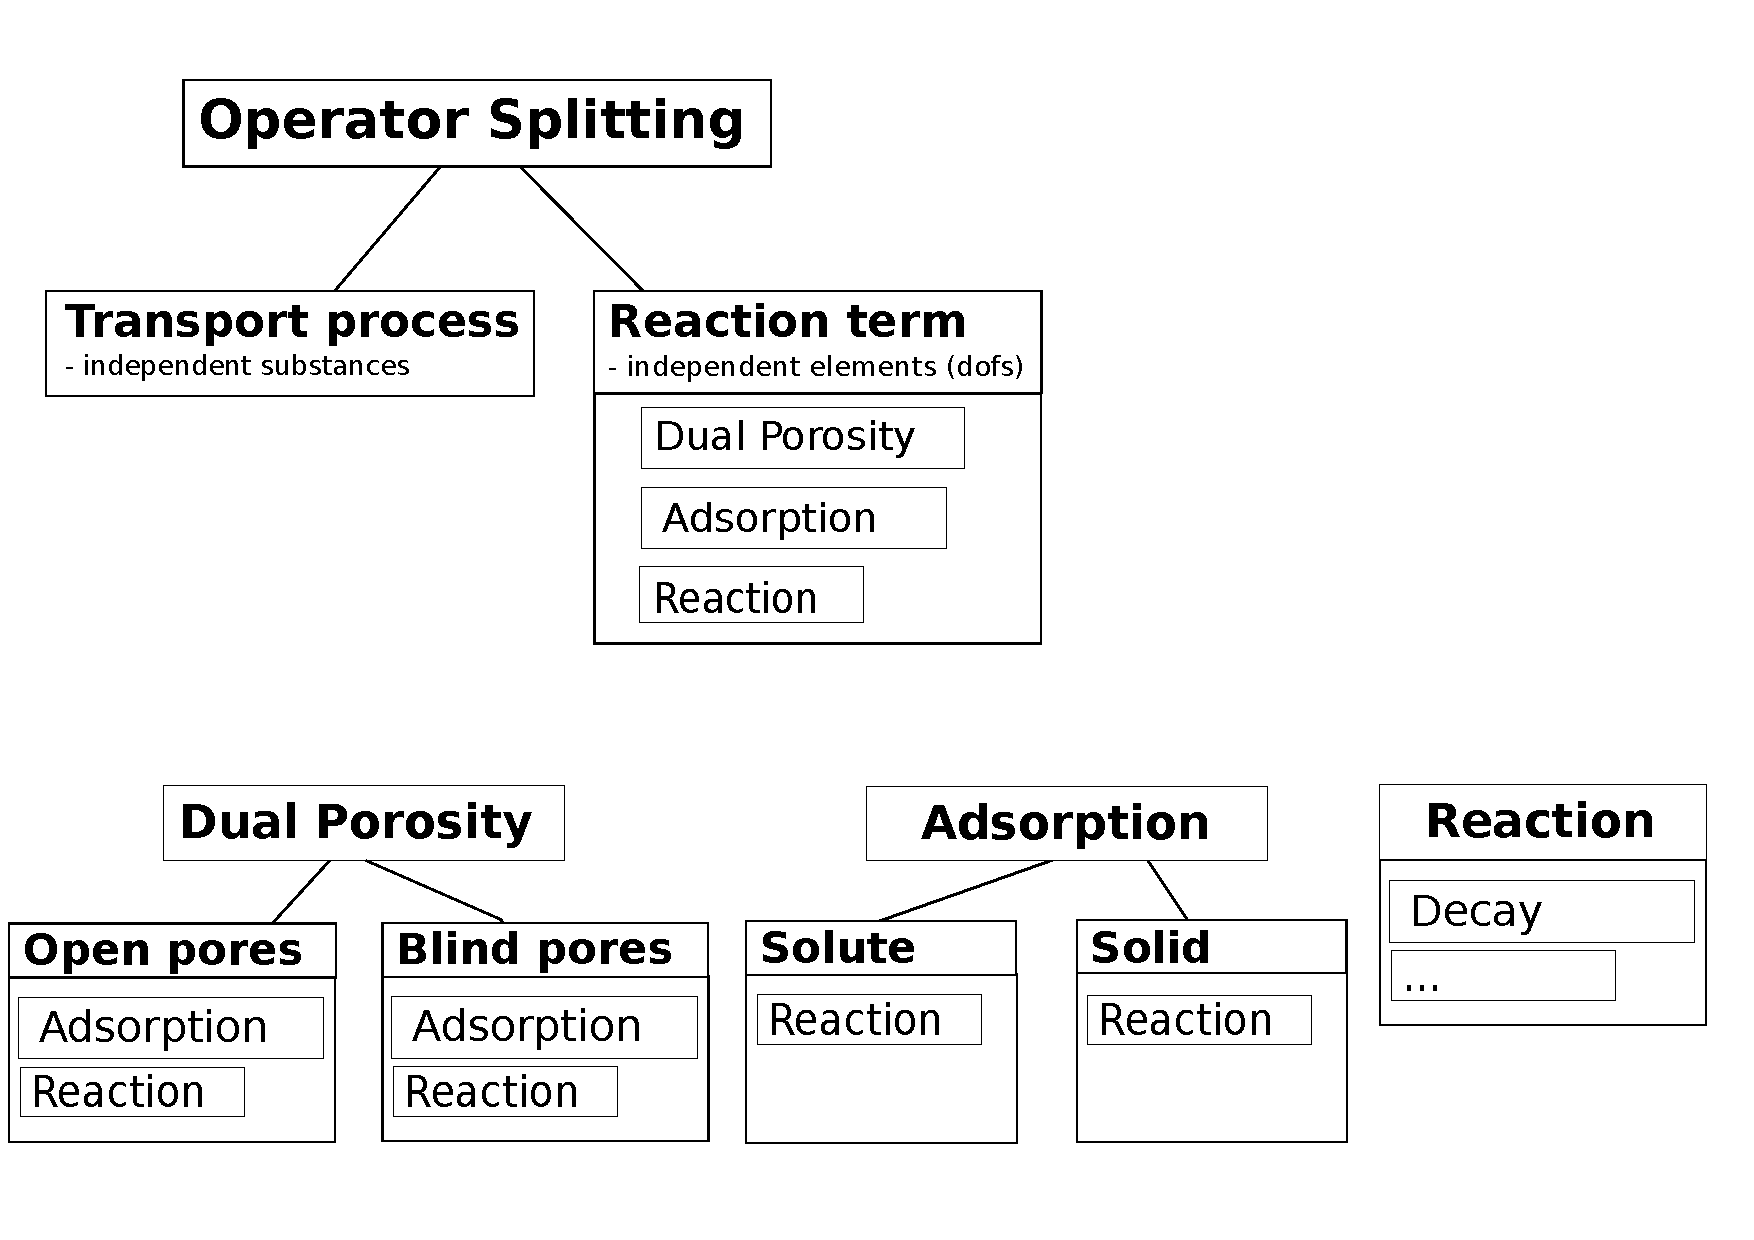
\includegraphics[width=\textwidth]{\fig/reaction_term.pdf}
  \caption{The scheme of the reaction term objects. The lines represents connections between different models. 
  The tables under model name include the possible models which can be connected to the model above.}
  \label{fig:reaction_term}
\end{figure}

The \emph{reaction} model acts only on the specified substances and computes exchange of concentration 
among them. It does not have its own output because it only changes the concentration of substances 
in the specified zone where the reaction takes place.
% See Section \ref{sec:linear_reactions} for thorough description.

The \emph{sorption} model describes the exchange of concentration of the substances between liquid and solid. It can be
followed by another \emph{reaction} that can run in both phases. The concentration in solid is an additional output 
of this model. See Subsection \ref{sec:sorp_math}.


The \emph{dual porosity} model, described in Subsection \ref{sec:dual_porosity}, introduces the so called immobile (or dead-end) pores in the matrix. 
The convection process operates only on the concentration of the substances in the mobile zone (open pores) 
and the exchange of concentrations from/to immobile zone is governed by molecular diffusion. This process can be followed by 
\emph{sorption} model and/or chemical \emph{reaction}, both in mobile and immobile zone. The immobile concentration is an
additional output.


\subsection{Dual Porosity} 
\label{sec:dual_porosity}

Up to now, we have described the transport equation for the single porosity model. The dual porosity model splits the mass into 
two zones -- the mobile zone and the immobile zone. Both occupy the same macroscopic volume, however on the microscopic scale, 
the immobile zone is formed by the dead-end pores, where the liquid is trapped and cannot pass through. The rest of the pore volume 
is occupied by the mobile zone. Since the liquid in the immobile pores is immobile, the exchange of the substance is only due 
to molecular diffusion. We consider simple nonequilibrium linear model:
\begin{subequations}
\label{eq:odes_dual_por}
\begin{align}
    \vartheta_m \partial_t c_m &= D_{dp} ( c_i - c_m), \label{eqn:dual_porosity_ode1}\\
    \vartheta_i \partial_t c_i &= D_{dp} ( c_m - c_i), \label{eqn:dual_porosity_ode2}
\end{align}
\end{subequations}
where $c_m$ is the concentration in the mobile zone, $c_i$ is the concentration in the immobile zone and
$D_{dp}$ is a \hyperA{DualPorosity-Data::diffusion-rate-immobile}{diffusion rate} between the zones.
$\vartheta_i$~denotes \hyperA{DualPorosity-Data::porosity-immobile}{porosity of the immobile zone} and 
$\vartheta_m = \vartheta$ the \hyperlink{TransportOperatorSplitting-Data::porosity::B}{mobile porosity} from 
transport equation \eqref{e:ADE}. One can also set non-zero \hyperA{DualPorosity-Data::init-conc-immobile}{initial 
concentration in the immobile zone} $c_i(0)$.

To solve the system of first order differential equation, we use analytic solution or Euler's method,
which are switched according to a given error tolerance. See subsection \ref{sec:num_dual_porosity} 
in numerical methods.
 

\subsection{Equilibrial Sorption}
\label{sec:sorp_math}

The simulation of monolayer, equilibrial sorption is based on the solution of two algebraic equations, namely the mass balance (in unit volume)
\begin{equation}
\label{eq:mass_balance_sorption}
\th \varrho_l c_l + (1-\th) \varrho_s M_s c_s = c_T = const.
\end{equation}
and an empirical sorption law
\begin{equation}
\label{eq:relation_cs_cl}
c_s = f(c_l),
\end{equation}
given in terms of the so-called isotherm $f$.
Its form is determined by the parameter \hyperA{Sorption-Data::sorption-type}{sorption type}:
\begin{itemize}
 \item ``$none$'': $f(c_l)=0$ (the sorption model returns zero concentration in solid);
 \item ``$linear$'': $f(c_l) = k_l c_l$;
 \item ``$freundlich$'': $f(c_l) = k_F c_l^{\alpha}$;
 \item ``$langmuir$'': $f(c_l) = k_L \frac{\alpha c_l}{1 + \alpha c_l}$.
       Langmuir isotherm has been derived from thermodynamic laws. $k_L$ denotes the maximal amount 
       of sorbing specie which can be kept in an unit volume of a bulk matrix. Coefficient $\alpha$ is 
       a fraction of sorption and desorption rate constant $\alpha = \frac{k_a}{k_d}$.
\end{itemize}

Notation:
\begin{itemize}
 \item In solid, $c_s = \frac{n}{m_s}$ [mol\,$\mathrm{kg}^{-1}$] is the fraction of the molar amount of the solute 
       adsorbed $n$ and the amount of the adsorbent $m_s$ (mass of solid), all in unit volume. The concentration
       in solid can be selected for \hyperA{Sorption::output-fields}{output}.
 \item In liquid, $c_l = \frac{m}{m_l}$ \units{}{}{} is the fraction of the amount of the solute $m$ and 
       the mass of liquid $m_l$, all in unit volume. The relation between $c_l$ and the concentration $c$ from 
       transport equation \eqref{e:ADE} is $c = c_l \varrho_l$.
 \item $\varrho_l$, $\varrho_s$ is the \hyperA{Sorption::solvent-density}{liquid (solvent) density} and 
       the \hyperA{Sorption-Data::rock-density}{solid (rock) density}, respectively.
 \item $M_s$ denotes the \hyperA{Substance::molar-mass}{molar mass} of a substance.
 \item \hyperA{Sorption-Data::isotherm-mult}{Multiplication parameters} are $k_i, i\in\{ l,F,L\}$ [mol\,$\mathrm{kg}^{-1}$].
 \item \hyperA{Sorption-Data::isotherm-other}{Additional parameter} $[\alpha] = 1$ can be set.
\end{itemize}

Non-zero \hyperA{Sorption-Data::init-conc-solid}{initial concentration} in the solid phase $c_s(0)$ can be set in the input record. 
Now, further denoting \[ \mu_l = \varrho_l \th, \quad \mu_s = M_s \varrho_s\cdot(1-\th), \]
and using \eqref{eq:relation_cs_cl}, the mass balance \eqref{eq:mass_balance_sorption} reduces to the equation
\begin{equation}
 c_T = \mu_l c_l + \mu_s f(c_l),
 \label{eq:nonlin_sorption}
\end{equation}
which can be either solved iteratively or using interpolation. See subsection \ref{sec:num_sorp_math} 
in numerical methods for details.

The units of $c_l$, $c_s$ and $k_i$ can vary in literature. To avoid misinterpretation, we derive (according
to Bowman~\cite{bowman_conversion_1982}) a conversion rule for Freundlich isotherm which will lead the user 
also in other cases, we believe. 

\paragraph{Units conversion.} Let us have $c$ \units{1}{-3}{}, the mass concentration in liquid, and $s$~[kg\,$\mathrm{kg}^{-1}$], 
the fraction of the amount of the solute adsorbed and the amount of the adsorbent in solid. 
The unit of $K$ follows from the dimensional analysis of $s=Kc^{\alpha}$:
\[[K] = \frac{\rm{kg}^{1-\alpha}\rm{m}^{3\alpha}}{\rm{kg}},\]
which we want to convert to $k_F$ [mol\,$\mathrm{kg}^{-1}$] in the formula $c_s=k_Fc_l^\alpha$.

The first step is a conversion of the mass of the solute to moles by dividing it by the
molar mass $M_s$. We then have the formula 
\begin{eqnarray}
s&=&Kc^{\alpha} \nonumber \\
\frac{s}{M_s} &=& K'\left(\frac{c}{M_s}\right)^\alpha, \label{eqn:sorp_molar_conc}\\
s &=& K'M_s^{1-\alpha}c^\alpha, \nonumber 
\end{eqnarray}
where $s=c_sM_s$ and $K'=KM_s^{\alpha-1}$ [$\rm{mol}^{1-\alpha}\rm{kg}^{-1}\rm{m}^{3\alpha}$] is a new constant,
distributing the molar concentration in liquid to the ratio of the molar mass and the amount of sorbent in solid.

The second step is introducing $c_l = \frac{c}{\varrho_l}$ into the formula \eqref{eqn:sorp_molar_conc}
\begin{equation}
c_s = K'\left(\frac{c_l \rho_l }{M_s}\right)^\alpha
= K' M_s^{-\alpha}\rho_l^{\alpha}c_l^\alpha 
= \left( K M_s^{-1}\rho_l^{\alpha} \right) c_l^\alpha,
\end{equation}
where we can denote 
\begin{equation}
k_F=K M_s^{-1}\rho_l^{\alpha},
\end{equation} 
which is the constant we are looking for. This can be also translated to the case of the linear isotherm, where
$\alpha=1$ and $[K] = \rm{kg}^{-1}\rm{m}^{3}$, and we get the conversion rule
\begin{equation}
k_l=K M_s^{-1}\rho_l.
\end{equation} 
The conversion of different prefixes of units are left on the user. One should be careful using the 
Freundlich isotherm, though, where the exponent $\alpha$ must not be forgotten.


\subsection{Sorption in Dual Porosity Model} 
\label{subsec:sorp_dual_por}
There are two parameters $\mu_l$ and $\mu_s$, scale of aqueous concentration and scale of sorbed concentration, respectively.  
There is a difference in computation of these in the dual porosity model because both work on different concentrations
and different zones.

Let $c_{ml}$ and $c_{ms}$ be concentration in liquid and in solid in the mobile zone, 
$c_{il}$ and $c_{is}$ be concentration in liquid and in solid in the immobile zone,
$\vartheta_m$ and $\vartheta_i$ be the mobile and the immobile porosity,
and $\varphi$ be the sorbing surface.

The sorbing surface in the mobile zone is given by
\begin{equation}
  \varphi = \frac{\vartheta_m}{\vartheta_m + \vartheta_i}, 
\end{equation}

while in the immobile zone it becomes
\[ 1 - \varphi = 1-\frac{\vartheta_m}{\vartheta_m + \vartheta_i} = \frac{\vartheta_i}{\vartheta_m + \vartheta_i}. \]

Remind the mass balance equation \eqref{eq:nonlin_sorption}.
In the dual porosity model, the scaling parameters $\mu_l$, $\mu_s$ are slightly different.
In particular, the mass balance in the mobile zone reads:
\begin{eqnarray}
 \begin{array}{l}
  c_T = \mu_l\cdot c_{ml} + \mu_s\cdot c_{ms},\\
  \mu_l = \varrho_l \cdot \vartheta_m, \\
  \mu_s = M_s \cdot\varrho_s\cdot(1-\vartheta_m - \vartheta_i)\varphi,
 \end{array}
 \label{eq:scale_params_m}
\end{eqnarray}
while in the immobile zone it has the form:
\begin{eqnarray}
 \begin{array}{l}
  c_T = \mu_l\cdot c_{il} + \mu_s\cdot c_{is},\\
  \mu_l = \varrho_l \cdot \vartheta_i, \\
  \mu_s = M_s \cdot\varrho_s\cdot(1-\vartheta_m - \vartheta_i)(1 - \varphi).
 \end{array}
 \label{eq:scale_params_i}
\end{eqnarray}


% TODO: Describe reactions, decays, numerical methods
% Copyright (C) 2007 Technical University of Liberec.  All rights reserved.
%
% Please make a following refer to Flow123d on your project site if you use the program for any purpose,
% especially for academic research:
% Flow123d, Research Centre: Advanced Remedial Technologies, Technical University of Liberec, Czech Republic
%
% This program is free software; you can redistribute it and/or modify it under the terms
% of the GNU General Public License version 3 as published by the Free Software Foundation.
%
% This program is distributed in the hope that it will be useful, but WITHOUT ANY WARRANTY;
% without even the implied warranty of MERCHANTABILITY or FITNESS FOR A PARTICULAR PURPOSE.
% See the GNU General Public License for more details.
%
% You should have received a copy of the GNU General Public License along with this program; if not,
% write to the Free Software Foundation, Inc., 59 Temple Place - Suite 330, Boston, MA 021110-1307, USA.

\normalsize

%%%%%%%%%%%%%%%%%        DOCUMENTATION OF GENERAL KINETIC REACTION FOR FUTURE -START           %%%%%%%%%%%%%%%

% \subsection{General Kinetic Reaction}
% \label{sec:kinetic}
% We consider a~system of $m$ stoichiometric reactions, each symbolically written as
% \begin{equation} \label{eqn:general_kinetic_reaction}
%   \sum\limits_{i=1}^{n_r} \nu_{rik}\chi_{i} \rightarrow \sum\limits_{i=1}^{n_r} \nu_{pik} \chi_{i},
% \end{equation}
% where 
% \begin{itemize}
%   \item $\nu_{rik}$ \units{}{}{} is the stoichiometric coefficient (number of moles) 
%         for reactant component $i$ in reaction $k$,
%   \item $\nu_{pik}$ \units{}{}{} is the stoichiometric coefficient
%         for product component $i$ in reaction $k$,
%   \item $n_r$ is the number of reaction components (both reactants and products),
%   \item $\chi_{i}$ represents the chemical symbol for the component $i$.
% \end{itemize}
% For the components that are not present in reaction, the stoichiometric coefficients are set
% $\nu_{rik}=0$ or $\nu_{pik}=0$.
% 
% The kinetics temperature dependence is introduce in modified Arrhenius model.
% The production rate of the component $i$ is then modeled as
% \begin{equation} \label{eqn:modified_arrhenius}
%   \frac{\d c_i}{\d t} = M_i \sum\limits_{k=1}^{m}\left( \nu_{pik}-\nu_{rik} \right) 
%   B_k \left(\frac{T}{T_{0k}}\right)^{\alpha_k} \exp\left(-\frac{\Delta E_k}{R_gT}\right)
%   \prod\limits_{j=1}^{n_r}\left(\frac{\rho_j}{M_j}\right)^{\nu_{rjk}},
% \end{equation}
% where
% \begin{itemize}
%   \item $c_i$ \units{1}{-3}{} is concentration of component $i$,
%   \item $M_i$, $M_j$ \units{1}{-3}{} is the molar mass of component $i$, or $j$ respectively,
%   \item $B_k$ \units{}{}{-1} is the collision-frequency factor (or preexponential factor) of reaction $k$,
%               it represents number of all particle collisions per second (not all necessarilly 
%               resulting in reaction),
%   \item $T$ [K] is the current absolute temperature,
%   \item $T_{0k}$ [K] is the reference absolute temperature, at which the number of particle collisions per second
%         is equal $B_k$,
%   \item $\alpha_k$ \units{}{}{} is the temperature exponent of the reaction $k$,
%   \item $\Delta E_k$ $[\textrm{Jmol}^{-1}]$ is the activation energy per mole,
%   \item $R_g = 8.3144$ $[\textrm{Jmol}^{-1}\textrm{K}^{-1}]$ is the universal gas constant,
%   \item $\rho_j$ \units{1}{-3}{} is the density of component $j$.
% \end{itemize}
% 
% To get rid of the unit dependence on the exponent, we divide the equation \eqref{eqn:modified_arrhenius} 
% by liquid density $\rho=\sum_{j=1}^{n_r}\rho_i$ and put $M_i$ under the exponent. Using
% \begin{equation}
%   \prod\limits_{j=1}^{n_r}\left( \frac{\rho_j M_i}{\rho M_j}\right)^{\nu_{rjk}} 
%   = \left(\frac{M_i}{\rho}\right)^{\sum_{j=1}^{n_r}\nu_{rjk}} 
%     \prod\limits_{j=1}^{n_r}\left( \frac{\rho_j}{M_j}\right),
% \end{equation}
% we obtain
% \begin{equation}
%   \frac{\d}{\d t}\left(\frac{c_i}{\rho}\right) = \sum\limits_{k=1}^{m}\left( \nu_{pik}-\nu_{rik} \right) 
%   B_k \left(\frac{T}{T_{0k}}\right)^{\alpha_k} \exp\left(-\frac{\Delta E_k}{R_gT}\right)
%   \left(\frac{M_i}{\rho}\right)^{1-\sum_{j=1}^{n_r}\nu_{rjk}} 
%   \prod\limits_{j=1}^{n_r}\left( \frac{\rho_j M_i}{\rho M_j}\right)^{\nu_{rjk}} 
% %   
% %   = \left(\frac{M_i}{\rho}\right)^{\sum_{j=1}^{n_r}\nu_{rjk}} 
% %     \prod\limits_{j=1}^{n_r}\left( \frac{\rho_j}{M_j}\right),
% \end{equation}

%%%%%%%%%%%%%%%%%          DOCUMENTATION OF GENERAL KINETIC REACTION FOR FUTURE -END           %%%%%%%%%%%%%%%

\subsection{Radioactive Decay}
\label{sec:decay}
The radioactive decay is one of the processes that can be modeled in the reaction term of the transport model.
This process is coupled with the transport using the operator splitting method.
It can run throughout all the phases, including the mobile and immobile phase of the liquid 
and also the sorbed solid phase, as it can be seen in figure \ref{fig:reaction_term}.

The radioactive decay of a~parent radionuclide A to a~nuclide B
%
\[ A\xrightarrow{k} B, \qquad A\xrightarrow{t_{1/2}} B \]
%
is mathematically formulated as a~system of first order differential equations
%
\begin{eqnarray} \label{eqn:halflife}
  \frac{\d c_A}{\d\tau} &=& -k c_A, \\
  \frac{\d c_B}{\d\tau} &=& k c_A,
\end{eqnarray}
%
where $k$ is the radioactive decay rate. Usually, the \hyperA{Decay::half-life}{half life} of the parent radionuclide $t_{1/2}$
is known rather than the rate. Relation of these can be derived:
%
% \begin{equation} \label{eqn:halflife}
%   k = - \frac{\ln 2}{t_{1/2}}.
% \end{equation}
\begin{eqnarray*}
    \frac{\d c_A}{\d\tau} &=& -k c_A\\
    \frac{\d c_A}{c_A} &=& -k \d\tau\\
    \int\limits_{c_A^0}^{c_A^0/2}\frac{\d c_A}{c_A} &=& -k\int\limits_{0}^{t_{1/2}} 1\d\tau\\
    \big[ \ln c_A\big]^{c_A^0/2}_{c_A^0} &=& -\big[k\tau\big]^{t_{1/2}}_{0}\\
%     \ln\frac{c_A^0}{2} - \ln c_A^0 &=& - k t_{1/2}\\
%     \ln 2 &=& k t_{1/2}\\
    k &=& \frac{\ln 2}{t_{1/2}}.
\end{eqnarray*}

Let us now suppose a~more complex situation. Consider substances (radionuclides) $A_1,\ldots, A_s$ which take 
part in a~complex radioactive chain, including branches, e.g.
\begin{center}
\begin{tabular}{rccll}
 $A_1\xrightarrow{k_1}A_2\xrightarrow{k_2}$ & $A_3$ & $ \xrightarrow{k_{34}}$ & $A_4\xrightarrow{k_4}$ & $A_8$ \\
 & $A_3$ & $\xrightarrow{k_{35}} A_5 \xrightarrow{k_{5}}$ & $A_4$ &\\
 & $A_3$ & \multicolumn{2}{c}{$\xrightarrow{k_{36}} A_6 \xrightarrow{k_{6}} A_7 \xrightarrow{k_{7}}$} & $A_8$
\end{tabular}
\end{center}
Now the problem turned into a~system of differential equations $\partial_t \vc{c}=\mathbf{D}\vc{c}$ with the following
matrix, generally full and nonsymmetric:
\[
\mathbf{D} = \begin{pmatrix} M_1 &     && \\ 
                                 & M_2 && \\
                                 && \ddots & \\
                  && & M_s \end{pmatrix}
             \begin{pmatrix} -k_1 &k_{21}& \cdots & k_{s1} \\ 
                  k_{12} & -k_2 & \cdots & k_{s2} \\
                  \vdots &\vdots& \ddots & \vdots \\
                  k_{1s} &k_{2s}& \cdots & -k_s \end{pmatrix}
             \begin{pmatrix} \frac{1}{M_1} &     && \\ 
                                 & \frac{1}{M_2} && \\
                                 && \ddots & \\
                  && & \frac{1}{M_s} \end{pmatrix},
\]
where $M_i$ is molar mass. We can then write
\begin{equation} \label{eqn:reaction_system_entries}
d_{ij} =
  \begin{cases}
  k_{ji} \frac{M_i}{M_j}, \quad i\neq j, \\
  -k_{ij}, \quad i=j. \\
  \end{cases}
\end{equation}
We denote the rate constant of the $i$-th radionuclide
\[
  k_i=\sum_{j=1}^{s}k_{ij}=\sum_{j=1}^{s}b_{ij}k_i
\]
which is equal to a~sum of partial rate constants $k_{ij}$. \hyperA{RadioactiveDecayProduct::branching-ratio}{Branching ratio} $b_{ij}\in(0,1)$ 
determines the distribution into different branches of the decay chain, holding $\sum_{j=1}^{s}b_{ij}=1$.

Notice, that physically it is not possible to create a~chain loop, so in fact one can permutate the vector of 
concentrations and rearrange the matrix $D$ into a~lower triangle matrix
\[
\mathbf{D} = \begin{pmatrix} d_{11} &  &  &  \\ 
                  d_{21} & d_{22} & &  \\
                  \vdots &\vdots& \ddots &  \\
                  d_{s1} &d_{s2}& \cdots & d_{ss} \end{pmatrix}.
\]
However, we do not do this and we do not search the reactions for chain loops.

The system of first order differential equations with constant coefficients is solved using one of the
implemented linear ODE solvers, described in section \ref{sec:num_slode}.


\subsection{First Order Reaction}
\label{sec:first_order_reaction}
First order kinetic reaction is another process that can take part in the reaction term. Similarly to the
radioactive decay, it is connected to transport by operator splitting method and can run in all the possible
phases, see figure \ref{fig:reaction_term}.

Currently, reactions with single reactant and multiple products (decays) are available in the software.
The mathematical description is the same as for the radioactive decay, it only uses 
\hyperA{Reaction::reaction-rate}{kinetic reaction rate} coefficient $k$ in the input instead of half life.







% OLD
% The software suppports linear chemical reactions in the transport operator splitting method. 
% The linear chemical reactions (we will recall them only as 'reactions' in this section) can desribe
% \begin{itemize}
%   \item first order kinetic chemical reactions
%   \item radioactive decays, their chains and also complex chains with branches.
% \end{itemize}
% In the first case, the kinetics of a~reaction is determined by a~kinetic constant \hyperA{Substep::kinetic}{$k$}. 
% In the second case, the radioactive decay is determined by the half life of the reactant 
% \hyperA{Substep::half-life}{$t_{1/2}$}. Both notations
% %
% \[ A\xrightarrow{k} B, \qquad A\xrightarrow{t_{1/2}} B \]
% %
% express the same reaction and are governed by the same first order differential equation 
% %
% \[ \frac{\d c_A}{\d\tau} = -kc_A = - \frac{\ln 2}{t_{1/2}}\, c_A. \]
% %
% The relation between $k$ and $t_{1/2}$ is derived below
% \begin{eqnarray*}
%     \frac{\d c_A}{\d\tau} &=& -k c_A\\
%     \frac{\d c_A}{c_A} &=& -k \d\tau\\
%     \int\limits_{c_A^0}^{c_A^0/2}\frac{\d c_A}{c_A} &=& -k\int\limits_{0}^{t_{1/2}} 1\d\tau\\
%     \big[ \ln c_A\big]^{c_A^0/2}_{c_A^0} &=& -\big[k\tau\big]^{t_{1/2}}_{0}\\
%     \ln\frac{c_A^0}{2} - \ln c_A^0 &=& - k t_{1/2}\\
%     \ln 2 &=& k t_{1/2}\\
%     k &=& \frac{\ln 2}{t_{1/2}}.
% \end{eqnarray*}
% 
% 
% 
% Lets consider to have a~narrow decay chain without branches. This kind of decay chain can be described by following equation
% \[
%  A\xrightarrow{t_{1/2,A}}B\xrightarrow{t_{1/2,B}}C\xrightarrow{t_{1/2,C}}D\xrightarrow{t_{1/2,D}}E,
% \]
% where letters $\{A,\ldots, E\}$ denotes isotopes contained in considered decay chain and ${t_{1/2},i},~i\in\{A,\ldots, E\}$ is a~symbol for a~half-life of $i$-th isotope.
% For a~simulation of radioactive decay and first order reactions matrix multiplication based approach has been developed. It has been based on an arrangement of all the data to matrices. The matrix ${\bf C}^k$ contains the information about concentrations of all species ($s$) in all observed elements ($e$). The upper index $k$ denotes $k$-th time step. The matrix ${\bf C}^k$ has the dimension $e\times s~( rows \times columns)$.
% The transport simulation is realized by matrix multiplication 
% \[
%   {\bf T}\cdot{\bf C}^k = {\bf C}^{k+1},
% \]
% where ${\bf T}$ is a~square, block-diagonal matrix, representing a~set of algebraic equations constructed from a~set of partial differential equations.
% When the simulation of the radioactive decay or the first order reaction is switched on, one step of
% simulation changes to 
% \[
%   {\bf T}\cdot{\bf C}^k\cdot{\bf R} = {\bf C}^{k+1},
% \]
% where ${\bf R}$ is a~square matrix with the dimension $(s \times s)$ . It is much easier to construct and to use ${\bf R}$ , than to include chemical influence to the transport
% matrix ${\bf T}$ , because the matrix ${\bf R}$ has usually a~simple structure and $s$ is much smaller than $e$. In the most simple case, when the order of identification numbers of isotopes in considered decay chain is the same as the order of identifiers of species transported by groundwater, then just two
% diagonals are engaged and the matrix R looks as follows:
% 
% \begin{tiny}\[
%    \begin{array}{l}
%     {\bf R} = \left(
%     \begin{array}{cccccc}
%      \left(\frac{1}{2}\right)^\frac{\Delta t}{t_{1/2,1}} & 1 - \left(\frac{1}{2}\right)^\frac{\Delta t}{t_{1/2,i}} & 0 & \hdots & \hdots & 0\\
%      0 & \left(\frac{1}{2}\right)^\frac{\Delta t}{t_{1/2,2}} & 1 - \left(\frac{1}{2}\right)^\frac{\Delta t}{t_{1/2,2}} & 0 & \ddots & 0 \\
%      \vdots & \ddots & \ddots & \ddots & \ddots & \vdots\\
%      0 & \ddots & 0 & \left(\frac{1}{2}\right)^\frac{\Delta t}{t_{1/2,n-2}} & 1 - \left(\frac{1}{2}\right)^\frac{\Delta t}{t_{1/2,n-2}} & 0 \\
%      0 & \hdots & \hdots & 0 & \left(\frac{1}{2}\right)^\frac{\Delta t}{t_{1/2,n-1}} & 1 - \left(\frac{1}{2}\right)^\frac{\Delta t}{t_{1/2,n-1}}\\
%      0 & \hdots & \hdots & 0 & 0 & 1
%     \end{array}\right)
%    \end{array}
% \]\end{tiny}
% 
% Every single $j$-th column, except the first one, includes the contribution $1 - \left(\frac{1}{2}\right)^\frac{\Delta t}{t_{1/2,j}},~j\in\{A,\ldots, E\}$ from $(j-1)$-th
% isotope with its half-life $t_{1/2,j-1}$. The term $\left(\frac{1}{2}\right)^\frac{\Delta t}{t_{1/2,j}}$ describes concentration decrease caused by the radioactive decay of $j$-th isotope itself. In general cases the matrix ${\bf R}$ can have much more complicated structure, especially when the considered decay chain has more branches.
% The implementation of the radioactive decay in Flow123D does not firmly include standard natural decay chain. Instead of that it is possible for a~user to define his/her decay chain.
% 
% It is also possible to simulate decay chains with branches as picture \ref{pic:dec_branches} shows.
% 
% \begin{figure}[htb]
%  \centering
%  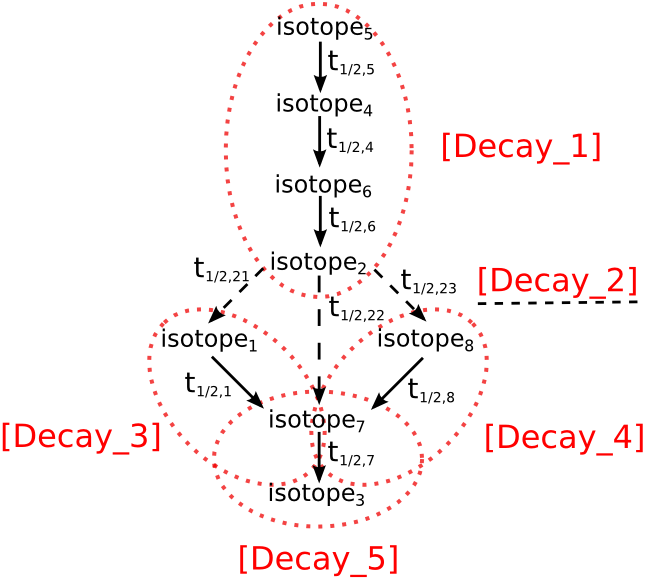
\includegraphics[width = 8cm]{\fig /decay_chain.png}
%  \caption{Decay chain with branches.}
%  \label{pic:dec_branches}
% \end{figure}
% 
% 
% When it comes to a~simulation of first order reactions, the kinetic constant is given as an input. 
% The description of a~kinetic chemical reaction has obviously two folowing forms
% \[
%   \begin{array}{l}
%     A\xrightarrow{k}B,\\
%     \frac{dc^A}{dt} = -k \cdot c^A.
%   \end{array}
% \]
% The first one description is a~standard chemical one. The second equation describes temporal decrease in amount of concentrations of the specie $c^A$. The constant $k$ is so called kinetic constant and for the case of a~first order reactions it is equal to so called reaction rate. The order of reaction with just one reactant is equal to the power of $c^A$ in partial diferential reaction.
% 
% For an inclusion of first order reaction into a~reaction matrix a~half-life needs to be computed from the corresponding kinetic constant $k$. The derivation follows
% \[
%   \begin{array}{l}
%     A\xrightarrow{k} B\\
%     \frac{dc^A}{d\tau} = -k\cdot c_A\\
%     \frac{dc^A}{c^A} = -k\cdot d\tau\\
%     \int\limits_{c^A_0/2}^{c^A_0}\frac{dc^A}{c^A} = -k\cdot\int\limits_{t_{1/2,A}}^{0} d\tau\\
%     \left[ ln c^A\right]_{c^A_0/2}^{c^A_0} = -[k\tau]_{t_{1/2,A}}^{0}\\
%     ln c^A_0 - \ln\frac{c^A_0}{2} = k\cdot t_{1/2,A}\\
% %     c^A (t) = c^A_0\cdot e^{-k\cdot t_{1/2,A}}\\
% %     {\bf substitution} \qquad c^A(t_{1/2,A}) = \frac{1}{2}\cdot c^A_0\\
% %     \frac{1}{2} c^A_0 = c^A_0\cdot e^{-k_1\cdot t_{1/2,A}}\\
%     \ln 2 = k \cdot t_{1/2,A}\\
%     t_{1/2,A} = \frac{ln 2}{k}
%   \end{array}                                                                                                                                                                                                                                                                                                            
% \]
% The matrix ${\bf R}$ is constructed in the same way as for the radioactive
% decay.


\section{Heat transfer}

Under the assumption of thermal equilibrium between the solid and liquid phase, the energy balance equation has the form\footnote{For lower dimensions this form can be derived as in Section \ref{sc:ad_on_fractures} using $w:=\delta\tilde s T$, $u:=T$, $\tn A:=\delta\lambda\tn I$, $\vc b:=\frac{\varrho_l c_l}{\tilde s}\vc w$.}
\[
    \partial_t\left(\delta \tilde s T \right) + \div(\varrho_l c_l T \vc q) - \div(\delta\Lambda\nabla T) = F^T + F^T_C.
\]
The principal unknown is the temperature $T$ [K].
Other quantities are:
\begin{itemize}
\item \hyperA{HeatTransfer-DG-Data::fluid-density}{$\varrho_l$}, \hyperA{HeatTransfer-DG-Data::solid-density}{$\varrho_s$} \units{1}{-3}{} is the density of the fluid and solid phase, respectively.
\item \hyperA{HeatTransfer-DG-Data::fluid-heat-capacity}{$c_l$}, \hyperA{HeatTransfer-DG-Data::solid-heat-capacity}{$c_s$} [J$\mathrm{kg}^{-1}\mathrm{K}^{-1}$] is the heat capacity of fluid and solid phase, respectively.
\item $\tilde s$ [J$\mathrm{m}^{-3}\mathrm{K}^{-1}$] is the volumetric heat capacity of the porous medium defined as
\[ \tilde s = \hyperA{HeatTransfer-DG-Data::porosity}{\th}\varrho_l c_l + (1-\th)\varrho_s c_s. \]
\item $\Lambda$ [W$\mathrm{m}^{-1}\mathrm{K}^{-1}$] is the thermal dispersion tensor:
\[ \Lambda = \Lambda^{cond} + \Lambda^{disp} \]
\[ \Lambda^{cond} = \left(\th \lambda_l^{cond} + (1-\th)\lambda_s^{cond}\right)\tn I, \]
\[ \Lambda^{disp} = \th \varrho_l c_l|\vc v|\left(\alpha_T\tn I + (\alpha_L-\alpha_T)\frac{\vc v\otimes\vc v}{|\vc v|^2}\right), \]
where \hyperA{HeatTransfer-DG-Data::fluid-heat-conductivity}{$\lambda_l^{cond}$}, \hyperA{HeatTransfer-DG-Data::solid-heat-conductivity}{$\lambda_s^{cond}$} [W$\mathrm{m}^{-1}\mathrm{K}^{-1}$] is the thermal conductivity of the fluid and solid phase, respectively, and \hyperA{HeatTransfer-DG-Data::disp-l}{$\alpha_L$}, \hyperA{HeatTransfer-DG-Data::disp-t}{$\alpha_T$} \units{}{1}{} is the longitudal and transverse dispersivity in the fluid.

\item $F^T$ [J$\mathrm{m}^{-d}\mathrm{s}^{-1}$] represents the thermal source:
\[ F^T = \delta \th F^T_l + \delta (1-\th) F^T_s, \]
\[ F^T_l = f_l^T + \varrho_l c_l \sigma^T_l(T-T_l), \]
\[ F^T_s = f_s^T + \varrho_s c_s \sigma^T_s(T-T_s), \]
where \hyperA{HeatTransfer-DG-Data::fluid-thermal-source}{$f_l^T$}, \hyperA{HeatTransfer-DG-Data::solid-thermal-source}{$f_s^T$} [W$\mathrm{m}^{-3}$] is the density of thermal sources in fluid and solid, respectively, \hyperA{HeatTransfer-DG-Data::fluid-ref-temperature}{$T_l$}, \hyperA{HeatTransfer-DG-Data::solid-ref-temperature}{$T_s$} [K] is a reference temperature and \hyperA{HeatTransfer-DG-Data::fluid-heat-exchange-rate}{$\sigma^T_l$}, \hyperA{HeatTransfer-DG-Data::solid-heat-exchange-rate}{$\sigma^T_s$} \units{}{}{-1} is the heat exchange rate.
\end{itemize}



\paragraph{Initial and boundary conditions.}
At time $t=0$ the temperature is determined by the initial condition
$$ T(0,\vc x) = \hyperA{HeatTransfer-DG-Data::init-temperature}{T_0}(\vc x). $$
Given the decomposition of $\partial\Omega_d$ into $\Gamma_I\cup\Gamma_D\cup\Gamma_N\cup\Gamma_R$ (see Section \ref{sc:transport_model}), we prescribe the following boundary conditions:
\begin{itemize}
\item Dirichlet:
\[ T = \hyperA{HeatTransfer-DG-Data::bc-temperature}{T_D} \mbox{ on }\Gamma_I^+\cup\Gamma_D, \]
\item Homogeneous Neumann:
\[ \left(\varrho_l c_l T \vc q - \delta\Lambda\nabla T\right)\cdot\vc n = 0 \mbox{ on }\Gamma_I^-, \]
\item Neumann:
\[ \left(\varrho_l c_l T \vc q - \delta\Lambda\nabla T\right)\cdot\vc n = \hyperA{HeatTransfer-DG-Data::bc-flux}{f_N} \mbox{ on }\Gamma_N, \]
\item Robin (Newton):
\[ \left(\varrho_l c_l T \vc q - \delta\Lambda\nabla T\right)\cdot\vc n = \hyperA{HeatTransfer-DG-Data::bc-robin-sigma}{\sigma_R}(T-\hyperA{HeatTransfer-DG-Data::bc-temperature}{T_D}) \mbox{ on }\Gamma_R. \]
\end{itemize}






\paragraph{Communication between dimensions.}
Denoting $T_{d+1}$, $T_d$ the temperature in $\Omega_{d+1}$ and $\Omega_d$, respectively, the communication on the interface between $\Omega_{d+1}$ and $\Omega_d$ is described by the quantity
\begin{equation}
  \label{e:inter_dim_flux_heat}
  q^T_{d+1,d} = \sigma^T_{d+1,d} \frac{\delta_{d+1}^2}{\delta_d}2\Lambda_d:\n\otimes\n ( T_{d+1} - T_d) + \begin{cases} \varrho_l c_l q^l_{d+1,d} T_{d+1} & \mbox{ if }q^l_{d+1,d}\ge 0,\\\varrho_l c_l q^l_{d+1,d} \frac{\tilde s_d}{\tilde s_{d+1}} T_d & \mbox{ if } q^l_{d+1,d}<0,\end{cases}
\end{equation}
where
\begin{itemize}
\item $q^T_{d+1,d}$ [W$\mathrm{m}^{-2}$] is the density of heat flux from $\Omega_{d+1}$ to $\Omega_d$,
\item \hyperA{HeatTransfer-DG-Data::fracture-sigma}{$\sigma^T_{d+1,d}$} \units{}{}{} is a transition parameter.
Its value determines the exchange of energy between dimensions due to temperature difference.
In general, it is recommended to leave the default value $\sigma^T=1$ or to set $\sigma^T=0$ (when exchange is due to water flux only).
\item $q^l_{d+1,d}=\vc q_{d+1}\cdot\vc n$ is the water flux from $\Omega_{d+1}$ to $\Omega_d$.
\end{itemize}
The communication between dimensions is incorporated as the total flux boundary condition for the problem on $\Omega_{d+1}$:
\begin{equation}
\label{e:heat_FC}
\left(\varrho_l c_l T \vc q - \delta\Lambda\nabla T\right)\cdot\vc n = q^T
\end{equation}
and a source term in $\Omega_d$:
\begin{equation}
F^T_{C3} = 0,\quad
F^T_{C2} = q^T_{32},\quad
F^T_{C1} = q^T_{21}.
\end{equation}




\paragraph{Energy balance.}
The heat equation satisfies the balance of energy in the following form:
$$ e(0) + \int_0^t s(\tau) \,d\tau - \int_0^t f(\tau) \,d\tau = e(t) $$
for any instant $t$ in the computational time interval.
Here
$$ e(t) := \sum_{d=1}^3\int_{\Omega^d}(\delta \tilde s T)(t,\vc x)\,d\vc x, $$
$$ s(t) := \sum_{d=1}^3\int_{\Omega^d}F_S^T(t,\vc x)\,d\vc x, $$
$$ f(t) := \sum_{d=1}^3\int_{\partial\Omega^d}\left(\varrho_l c_l T\vc q - \delta\Lambda\nabla T\right)(t,\vc x)\cdot\vc n \,d\vc x $$
is the energy [J], the volume source [J$\mathrm{s}^{-1}$] and the energy flux [J$\mathrm{s}^{-1}$] at time $t$, respectively.
The energy, flux and source on every geometrical region is calculated at each computational time step and the values together with the control sums are written to the file \texttt{mass\_balance.txt}.









\chapter{Numerical Methods}
\label{chapter:numerical}
% TODO: Update numerical topics
\section{Diagonalized Mixed-Hybrid Method}
\def\mr{\mathring}
Model of flow described in section \ref{sec:darcy_flow} is solved by
the mixed-hybrid formulation (MH) of the finite element method.
As in the previous chapter, let
$\tau$ be the time step and $\mathcal T_d$ a regular simplicial partition of $\Omega_d$, $d=1,2,3$.
Denote by $\vc W_d(T_d)\subset \vc H(div,T_d)$
 the space of Raviart-Thomas functions of order zero ($RT_0$) on an element $T_d\in 
\mathcal T_d$.
We introduce the following spaces:
\[
    \vc W =  \vc W_1 \times \vc W_2 \times \vc W_3,\quad
    \vc W_d = \prod_{T_d\in \mathcal T_d} \vc W_d(T_d),
\]
\begin{equation}
Q=Q_{1}\times Q_{2}\times Q_{3},
\quad
Q_{d}=L^{2}\left(  \Omega_{d}\right).
\end{equation}
For every $T_d\in \mathcal T_d$ we define the auxiliary space of values on interior sides of $T_d$:
\begin{equation}
    \mr Q(T_d)=\left\{  \mr q\in 
    L^{2}(\partial T_d \setminus  \partial\Omega_d^D):
    \mr q =\vc w\cdot \vc n|_{\partial T_d},
    \vc w\in\vc W_d%
    \right\}.
\end{equation}
Further we introduce the space of functions defined on interior sides that do not coincide with elements of the lower dimension:
\begin{equation}
    \mr Q_d=\Big\{
        \mr q\in\prod_{T \in \mathcal T_d} \mr Q(T);
        \ \mr q|_{\partial T}=\mr q|_{\partial \tilde T}%
        \quad\text{on the side }F=\partial T\cap\partial \tilde T
        \quad\text{ if }F\cap\Omega_{d-1}=\emptyset
    \Big\}.
\end{equation}
Finally we set $\mr Q = \mr Q_1 \times \mr Q_2 \times \mr Q_3$.

The \emph{mixed-hybrid method} for the unsteady Darcy flow reads as follows.
We are looking for a trio $(\mathbf{u},h,\mr h)  
\in \vc W\times Q\times\mr Q$ which satisfies the saddle-point problem:
\begin{align}
    a(\vc u,\vc v)  +b(\vc v, p) + \mr b(\vc v, \mr p)
        &=\langle g,\vc v \rangle, \qquad\forall \vc v\in \vc W,
        \label{eq:hybrid-frac-1}\\
    b(\vc u, q ) + \mr b( \vc u, \mr q) - c(p, \mr p, q, \mr q)
        &= \langle f, (q,\mr q) \rangle,
        \qquad\forall q\in Q,\ \mr q\in \mr Q, 
        \label{eq:hybrid-frac-2}
\end{align}
where
\begin{align}
    \label{eq:weak_term_a}
    a(\vc u, \vc v) &= \sum_{d=1}^{3}\sum_{T\in \mathcal T_d}
    \int_{T} \frac{1}{\delta_{d}}\tn K_{d}^{-1} 
    \vc u_d\cdot \vc v_d\,dx,
    \\
    \label{eq:weak_term_b}
    b(\vc u, q)  &= -\sum_{d=1}^{3}\sum_{T\in \mathcal T_d}
    \int_{T} q_d\,\div \vc u_d\,dx,
    \\
    \label{eq:weak_term_bf}
    \mr b(\vc u, \mr q)   &= \sum_{d=1}^{3}\sum_{T\in \mathcal T_d}
    \int_{\partial T\setminus\partial\Omega_{d}}
        \mr q|_{\partial T} ( \vc u_d\cdot\vc n)\,ds,
    \\
    \label{eq:weak_term c}
    c(h, \mr h, q, \mr q) &= c_f(h, \mr h, q, \mr q) 
    + c_t(h, \mr h, q, \mr q) + c_R(\mr h, \mr q)
    \\
    c_f(h, \mr h, q, \mr q)&=\sum_{d=2,3}\sum_{T\in \mathcal T_d}
        \int_{\partial T \cap\Omega_{d-1}} \sigma_{d} 
        (p_{d-1} - \mr p_d)(q_{d-1} - \mr q_d)\,ds
    \\
    c_t(h, \mr h, q, \mr q)&= \sum_{d=1}^{3}\sum_{T\in \mathcal T_d}
        \int_{T} \frac{\delta_d S_d}{\tau} h_d q_d\,dx,
    \\    
    c_R(\mr h, \mr q)&= \sum_{d=1}^{3}\sum_{T\in \mathcal T_d}
    \int_{\partial T\cap\Gamma_{d}^{TF}}
        \sigma_d^R\, h_d \mr q_d \,ds,
    \\
    \langle g, \vc v \rangle  & =
    -\sum_{d=1}^{3}\sum_{T\in\mathcal T_d}
    \int_{\partial T\cap\partial\Omega_N} 
        p_d^D\, (\vc v \cdot \vc n)  \,ds,
    \\
    \langle f, q \rangle  &=
    -\sum_{d=1}^{3}\int_{\Omega_d} \delta_{d}\,f_d\,q_{d}\,dx,
    \\
        &\phantom{=}-
    \sum_{d=1}^{3}\sum_{T\in\mathcal T_d}
    \int_{\partial T\cap\Gamma_d^{TF}} 
        q_d^N \mr q_d + \sigma_d^R\, h_d^R \mr q_d\,ds
    \\
        &\phantom{=}-c_t(\tilde h, \mr{\tilde{h}}, q, \mr q).
    \label{eq:weak_term_f}%    
\end{align}
All quantities are meant in time $t$, only $\tilde h$ is the pressure head in time $t-\tau$.

The advantage of the mixed-hybrid method is that the set of equations $\eqref{eq:hybrid-frac-1} - 
\eqref{eq:hybrid-frac-2}$ can be reduced by eliminating the unknowns $\vc u$ and $q$
to a sparse positive definite system for $\mr q$.
This equation can then be efficiently solved using a~preconditioned conjugate gradient method.
Unfortunately, it appears that the resulting system does not satisfy the discrete maximum principle
 which in particular for short time steps $\tau$ can lead to unphysical oscillations.
One possible solution is the diagonalization of the method (lumped mixed-hybrid method, LMH)
 proposed in \cite{younes_2006}.
This method was implemented in Flow123d as well.
It consists in replacing the form $c_t$ by
\[
    c_t(h, \mr h, q, \mr q)= \sum_{d=1}^{3}\sum_{T\in \mathcal T_d}
        \sum_{i=1}^{d+1} \alpha_{T,i} \abs{T} \frac{\delta_d S_d}{\tau} 
        \left(\mr h|_{S_{T,i}}\,  \mr q|_{S_{T,i}}\right),
\]
and the source term $\sum_{d=1}^{3}\int_{\Omega_d} \delta_{d}\,f_d\,q_{d}\,dx$ by
\[
    \sum_{d=1}^{3}\sum_{T\in \mathcal T_d}
        \sum_{i=1}^{d+1} \alpha_{T,i} \abs{T} \delta_d f_d\,
        \mr q|_{S_{T,i}},
\]
where $\abs{T}$ is the size of an element $T$, $S_{T,i}$ is the $i$-th side of $T$, and 
$\mr h|_{S_{T,i}}$ is the degree of freedom on the side $S_{T,i}$. 
Weights $\alpha_{T,i}$ can be chosen to be $1/(d+1)$. 
After solving the set of equations it is necessary to modify the velocity field $\vc u$
 by adding the time term.
This modified system already satisfies the discrete maximum principle
 and does not produce oscillations.
Figure \ref{fig:LMH} shows a comparison of the results
 using conventional MH scheme and LMH scheme.
At the MH scheme one can observe oscillations in the wavefront
 where the minimum value is significantly less than zero.

\begin{figure}
    \begin{center}
       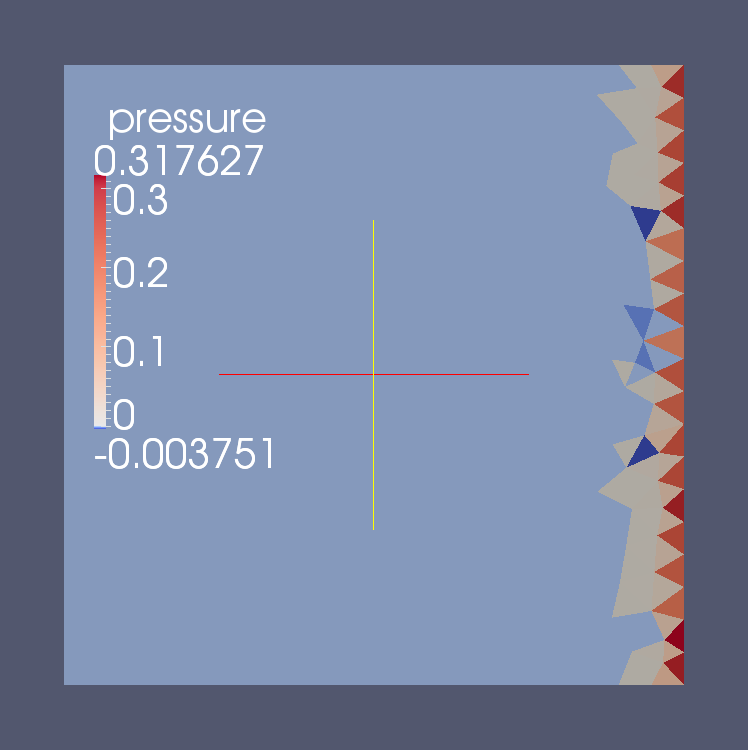
\includegraphics[width=0.4\textwidth]{figures/MH.png}
       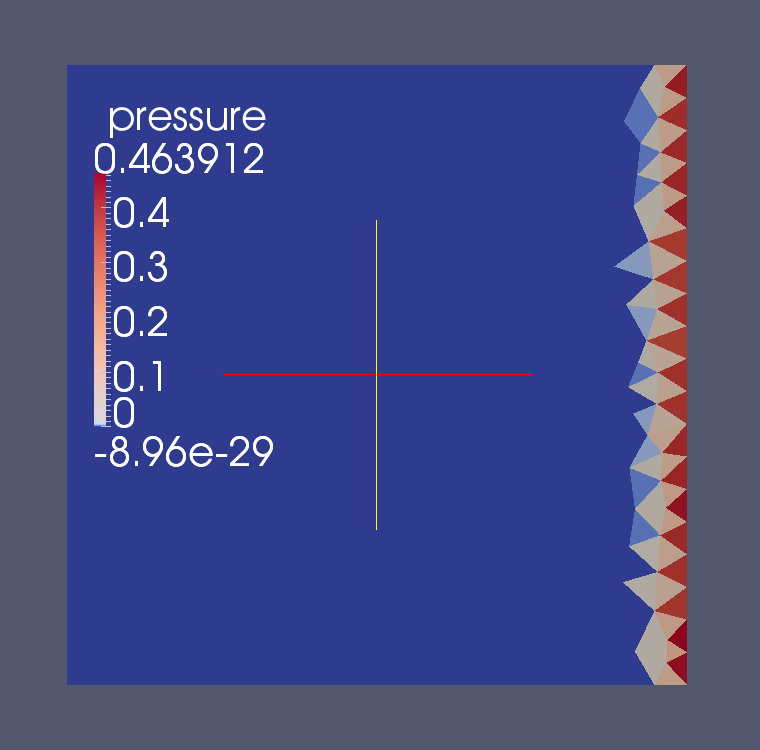
\includegraphics[width=0.405\textwidth]{figures/LMH.png}        
    \end{center}
    \caption{Comparison of MH (left) and LMH scheme (right), $\tau=10^{-4}$.}
    \label{fig:LMH}
\end{figure}

\section{Mixed-Hybrid Method on Non-conforming Mixed Meshes}
The coupling for a non-conforming mixed mesh introduces a new term $c_F(h, \mr h, q, \mr q)$ to the formulation $\eqref{eq:hybrid-frac-1} - 
\eqref{eq:hybrid-frac-2}$ similar to the term $c_f$ responsible for the compatible coupling. We distinguish coupling of codimension $d'=1$, i.e. 2d in 3d and 1d in 2d,
and coupling of codimension $d'=0$, 2d-2d in 3d space and 1d-1d in 2d space. This way we split $c_F$ into
\[
    c_F= \sum_{d'=0,1} \sum_{d=1,2} c_F,d',d
\]
All these termse share common form:
For codimension 1 we have:
\end{equation*}
  c_F,1,d(h, \mr h, q, \mr q) &&=  \int_{T^d} \sigma_d
                \big(R({\mr{h}_d}) - T({\mr{h}_{d+1}}) \big)
                 \big(R({\mr{\phi}_d}) - T({\mr{\phi}_{d+1}}) \big),
\end{equation*}
where $R$ is the reconstruction operator of the pressure he and $T$ is the trace approximation.






%%%%%%%%%%%%%%%%%%%%%%%%%%%%%%%%%%%%%%%%%%%%%%%%%%%%%%%%%%%%%%%%%%%%%
\section{Discontinuous Galerkin Method}
\label{sc:dg}

\def\Eh{\mathcal E_d}       % edges of \Th
\def\Ehb{\mathcal E_{d,B}}  % edges of \Th on boundary
\def\Ehcom{\mathcal E_{d,C}}         % edges of \Th on interface with lower dimension
\def\Ehdir{\mathcal E_{d,D}}         % Dirichlet edges of \Th
\def\Ehint{\mathcal E_{d,I}}       % interior edges of \Th
\def\Ehneu{\mathcal E_{d,N}}         % Neumann or Robin edges of \Th
\def\Ngh{\mathcal N_d}
\def\avg#1{\left\{#1\right\}}
\def\jmp#1{[#1]}
\def\wavg#1#2#3{\avg{#1}_{#2,#3}^\omega}
\def\Td{\mathcal T_d}


Models for solute transport and heat transfer described in sections \ref{sc:transport_model} and \ref{sc:heat} are collectively formulated
 as a system of abstract advection-diffusion equations on domains $\Omega_d$, $d=1,2,3$,
 connected by communication terms.
Consider for $d=1,2,3$ the equation 
\begin{subequations}
 \label{eq:abstr_system}
 \begin{equation}
  \partial_t u_d + \div(\vc b u_d) - \div(\tn A\nabla u_d) = f^0+f^1(u^S-u_d) + q(u_{d+1},u_d) \mbox{ in }(0,T)\times\Omega_d
 \end{equation}
 with initial and boundary conditions
 \begin{align}
  u_d(0,\cdot) &= u^0 &&\mbox{ in }\Omega_d,\\
  \label{eq:bc_abstr_dir} u_d &= u^D &&\mbox{ on }(0,T)\times\Gamma^D_d,\\
  \label{eq:bc_abstr_neu} (\vc b u_d-\tn A\nabla u_d)\cdot\vc n &= f^N + \sigma^R(u_d - u^D) &&\mbox{ on }(0,T)\times\Gamma^N_d,\\
  (\vc b u_d-\tn A\nabla u_d)\cdot\vc n &= q(u_d,u_{d-1}) &&\mbox{ on } (0,T)\times\Gamma^C_d,
 \end{align}
 where
 \[ \Gamma^C_d:=\overline\Omega_d\cap\overline\Omega_{d-1}. \]
 The communication term $q(u_{d+1},u_d)$ has the form
 \begin{equation}
 \label{eq:com_term_abstr_system}
  q(u_{d+1},u_d) =
  \begin{cases}
      \alpha u_{d+1} + \beta u_d
    & \mbox{ in }\Gamma^C_{d+1},~d=1,2,\\ 0
    & \mbox{ on }\Omega_d\setminus\Gamma^C_{d+1},~d=1,2,\mbox{ and for }d=0,3.
  \end{cases}
 \end{equation}
\end{subequations}
System \eqref{eq:abstr_system} is spatially discretized by the discontinuous Galerkin method
 with weighted averages,
 which was derived for the case of one domain in \cite{ern_stephansen_zunino}
 (for a posteriori estimate see \cite{ern2010guaranteed}).
For time discretization we use the implicit Euler method.

Let $\tau$ denote the time step.
For a regular splitting $\Td$ of $\Omega^d$, $d=1,2,3$, into simplices we define the following sets of element sides:
\begin{align*}
 &\Eh &&\mbox{sides of all elements in $\Td$ (i.e. triangles for $d=3$, lines for $d=2$ and nodes for $d=1$)},\\
 &\Ehint &&\mbox{interior sides (shared by 2 or more $d$-dimensional elements)},\\
 &\Ehb &&\mbox{outer sides (belonging to only one element)},\\
 &\Ehdir(t) &&\mbox{sides, where the Dirichlet condition \eqref{eq:bc_abstr_dir} is given},\\
 &\Ehneu(t) &&\mbox{sides, where the Neumann or Robin condition \eqref{eq:bc_abstr_neu} is given},\\
 &\Ehcom &&\mbox{sides coinciding with $\Gamma^C_d$}.
\end{align*}
For an interior side $E$ we denote by $\Ngh(E)$ the set of elements that share $E$ (notice that 1D and 0D sides can be shared by more than 2 elements).
For an element $T\in\Ngh(E)$ we denote $q_T:=(\vc b\cdot\vc n)_{|T}$ the outflow from $T$,
and define $\Ngh^-(E):=\{T\in\Ngh(E)\where q_T\le 0\}$, $\Ngh^+(E):=\{T\in\Ngh(E)\where q_T>0\}$
the sets of all outflow and inflow elements, respectively.
For every pair $(T^+,T^-)\in \Ngh^+(E)\times\Ngh^-(E)$ we define the flux from $T^+$ to $T^-$ as
$$ q_{T^+\to T^-} := \frac{q_{T^+} q_{T^-}}{\sum_{T\in\Ngh^-(E)}{q_T}}.$$
We select arbitrary element $T_E\in\Ngh(E)$ and define $\n_E$ as the the unit outward normal vector to $\partial T_E$ at $E$.
The jump in values of a function $f$ between two adjacent elements $T_1,T_2\in\Ngh(E)$ is defined by $\jmp{f}_{T_1,T_2}=f_{|T_{1|E}}-f_{|T_{2|E}}$,
 similarly we introduce the average $\avg{f}_{T_1,T_2}=\frac12(f_{|T_{1|E}} + f_{|T_{2|E}})$
 and a weighted average $\wavg{f}{T_1}{T_2}=\omega f_{|T_{1|E}} + (1-\omega) f_{|T_{2|E}}$.
The weight $\omega$ is selected in a specific way (see \cite{ern_stephansen_zunino})
 taking into account the possible inhomogeneity of the tensor $\tn A$.

% Let us fix one substance and the space dimension $d$.
For every time step $t_k=k\tau$ we look for the discrete solution $u^{k}=(u_1^{k},u_2^{k},u_3^{k})\in V$, where
$$ V=\prod_{d=1}^3 V_d \quad\mbox{ and }\quad V_d = \{v:\overline{\Omega^d}\to\R\where v_{|T}\in P_p(T)~\forall T\in\Td\} $$
are the spaces of piecewise polynomial functions of degree at most $p$ on elements $\Td$,
 generally discontinuous on interfaces of elements.
The initial condition for $u_d^{0}$ is defined as the $L^2$-projection of $u^0$ to $V_d$.
For $k=1,2,\ldots$, $u^{k}$ is given as the solution of the problem
\begin{equation*}
 \frac1\tau\sc{u^{k}-u^{k-1}}{v}_{V} + a^{k}(u^{k},v) = b^{k}(v) \quad \forall v\in V.
\end{equation*}
Here $\sc{f}{g}_{V}=\sum_{d=1}^d\sc{f}{g}_{\Omega^d}$, $\sc{f}{g}_{\Omega^d}=\int_{\Omega^d} f g$,
 and forms $a^{k}$, $b^{k}$
 are defined as follows:
\begin{multline}
\label{eq:df_ak_abstr_sys}
  a^{k}((u_1,u_2,u_3),(v_1,v_2,v_3))\\
   = \sum_{d=1}^3\bigg( a^{k}_d(u_d,v_d)
    - \sc{q(u_{d+1},u_d)}{v_d}_{\Omega^d}
    - \sum_{E\in\Ehcom^d(t_k)}\sc{q(u_d,u_{d-1})}{v_d}_E \bigg),
\end{multline}
\begin{equation}
\label{eq:df_bk_abstr_sys}
b^{k}((v_1,v_2,v_3)) = \sum_{d=1}^3 b^{k}_d(v_d), \mbox{\hspace{11.7cm}}
\end{equation}
\begin{align*}
 a^{k}_d(u,v) = &\sc{\tn A\nabla u}{\nabla v}_{\Omega^d}
 - \sc{\vc b u}{\nabla v}_{\Omega^d} + \sc{f^1 u}{v}_{\Omega^d}\\
 &- \sum_{E\in\Ehint^d}\sum_{\substack{T_1,T_2\in\Ngh(E)\\T_1\neq T_2}}\bigg(\sc{\wavg{\tn A\nabla u}{T_1}{T_2}\cdot\n_E}{\jmp{v}_{T_1,T_2}}_E + \Theta\sc{\wavg{\tn A\nabla v}{T_1}{T_2}\cdot\n_E}{\jmp{u}_{T_1,T_2}}_E \\
 &- \gamma_E\sc{\jmp{u}_{T_1,T_2}}{\jmp{v}_{T_1,T_2}}_E \bigg)
 - \sum_{E\in\Ehint^d}\sum_{\substack{T^+\in\Ngh^+(E)\\T^-\in\Ngh^-(E)}}\sc{q_{T^+\to T^-}\avg{u}_{T^+,T^-}}{\jmp{v}_{T^+,T^-}}_E\\
%  & + \sum_{E\in\Ehb^d}\sc{\vc b\cdot\n u}{v}_E
 &+ \sum_{E\in\Ehdir^d(t_k)}\bigg(\gamma_E\sc{u}{v}_E + \sc{\vc b\cdot\n u}{v}_E - \sc{\tn A\nabla u\cdot\vc n}{v}_E - \Theta\sc{\tn A\nabla v\cdot\vc n}{u}_E\bigg)\\
 &+ \sum_{E\in\Ehneu^d(t_k)}\sc{\sigma^R u}{v}_E,\\
% \end{multline*}
% 
% \begin{equation*}
 b^{k}_d(v) = &\sc{f^0+f^1 u^S}{v}_{\Omega^d} + \sum_{E\in\Ehdir^d(t_k)}\bigg(\gamma_E\sc{u^D}{v}_E - \Theta\sc{u^D}{\tn A\nabla v\cdot\vc n}_E\bigg)\\
 & + \sum_{E\in\Ehneu^d(t_k)}\sc{\sigma^R u^D-f^N}{v}_E.
\end{align*}
The Dirichlet condition is here enforced by a penalty with an arbitrary parameter $\gamma_E>0$;
 its value influences the level of solution's discontinuity.
For $\gamma_E\to+\infty$ we obtain asymptotically (at least formally) the finite element method.
The constant $\Theta$ can take the values $-1$, $0$ or $1$,
 where $-1$ corresponds to the nonsymetric, $0$ to the incomplete and $1$ to the symetric variant of the discontinuous Galerkin method.




\section{Finite Volume Method for Convective Transport}

In the case of the purely convective solute transport ($\tn D=0$), problem \eqref{eq:abstr_system} is replaced by:
\begin{subequations}
 \label{eq:abstr_system_conv}
 \begin{align}
  \partial_t u_d + \div(\vc b u_d) &= f^0+f^1(u^S-u_d) + q(u_{d+1},u_d) &&\mbox{ in }(0,T)\times\Omega_d,\\
  u_d(0,\cdot) &= u^0 &&\mbox{ in }\Omega_d,\\
  \label{eq:bc_abstr_neu} (\vc b\cdot\vc n) u_d &= (\vc b\cdot\vc n) u^D &&\mbox{ on }\Gamma_d^I,
 \end{align}
\end{subequations}
 where
 \[ \Gamma_d^I:=\{(t,\vc x)\in(0,T)\times\partial\Omega_d\where \vc b(t,\vc x)\cdot\vc n(\vc x)<0\}. \]
 The communication term $q(u_{d+1},u_d)$ has the same structure as in \eqref{eq:com_term_abstr_system}.

The system is discretized by the cell-centered finite volume method combined with the explicit Euler time discretization.
Using the notation of Section \ref{sc:dg}, we consider the space $V$ of piecewise constants on elements and define the discrete problem:
\begin{equation*}
 \frac1\tau\sc{u^{k}-u^{k-1}}{v}_{V} + a^{k-1}(u^{k-1},v) = b^{k-1}(v) \quad \forall v\in V,
\end{equation*}
where the forms $a^k$ and $b^k$ are defined in \eqref{eq:df_ak_abstr_sys}-\eqref{eq:df_bk_abstr_sys} and $a^k_d$, $b^k_d$ now have simplified form:
\begin{align*}
 a^{k}_d(u,v) = & -\sum_{T_i\in\Td}\left(\sc{(\vc b\cdot\vc n)^+u}{v}_{\partial T_i} + \sum_{T_j\in\Td}\sc{q_{T_j\to T_i}u}{v}_{\partial T_i\cap\partial T_j} \right),\\
 b^{k}_d(v) = &\sc{f^0+f^1(u^S-u^{k-1}_d)^+}{v}_{\Omega^d} + \sum_{T_i\in\Td}\sc{(\vc b\cdot\vc n)^-u^D}{v}_{\partial T_i\cap\partial\Omega_d}.
\end{align*}
The above formulation corresponds to the upwind scheme, ideal mixing in case of multiple elements sharing one side, and explicit treatment of linear source term.

% \input convection


\section{Solution Issues for Reaction Term}

% % Copyright (C) 2007 Technical University of Liberec.  All rights reserved.
%
% Please make a following refer to Flow123d on your project site if you use the program for any purpose,
% especially for academic research:
% Flow123d, Research Centre: Advanced Remedial Technologies, Technical University of Liberec, Czech Republic
%
% This program is free software; you can redistribute it and/or modify it under the terms
% of the GNU General Public License version 3 as published by the Free Software Foundation.
%
% This program is distributed in the hope that it will be useful, but WITHOUT ANY WARRANTY;
% without even the implied warranty of MERCHANTABILITY or FITNESS FOR A PARTICULAR PURPOSE.
% See the GNU General Public License for more details.
%
% You should have received a copy of the GNU General Public License along with this program; if not,
% write to the Free Software Foundation, Inc., 59 Temple Place - Suite 330, Boston, MA 021110-1307, USA.

\normalsize

%%%%%%%%%%%%%%%%%        DOCUMENTATION OF GENERAL KINETIC REACTION FOR FUTURE -START           %%%%%%%%%%%%%%%

% \subsection{General Kinetic Reaction}
% \label{sec:kinetic}
% We consider a system of $m$ stoichiometric reactions, each symbolically written as
% \begin{equation} \label{eqn:general_kinetic_reaction}
%   \sum\limits_{i=1}^{n_r} \nu_{rik}\chi_{i} \rightarrow \sum\limits_{i=1}^{n_r} \nu_{pik} \chi_{i},
% \end{equation}
% where 
% \begin{itemize}
%   \item $\nu_{rik}$ \units{}{}{} is the stoichiometric coefficient (number of moles) 
%         for reactant component $i$ in reaction $k$,
%   \item $\nu_{pik}$ \units{}{}{} is the stoichiometric coefficient
%         for product component $i$ in reaction $k$,
%   \item $n_r$ is the number of reaction components (both reactants and products),
%   \item $\chi_{i}$ represents the chemical symbol for the component $i$.
% \end{itemize}
% For the components that are not present in reaction, the stoichiometric coefficients are set
% $\nu_{rik}=0$ or $\nu_{pik}=0$.
% 
% The kinetics temperature dependence is introduce in modified Arrhenius model.
% The production rate of the component $i$ is then modeled as
% \begin{equation} \label{eqn:modified_arrhenius}
%   \frac{\d c_i}{\d t} = M_i \sum\limits_{k=1}^{m}\left( \nu_{pik}-\nu_{rik} \right) 
%   B_k \left(\frac{T}{T_{0k}}\right)^{\alpha_k} \exp\left(-\frac{\Delta E_k}{R_gT}\right)
%   \prod\limits_{j=1}^{n_r}\left(\frac{\rho_j}{M_j}\right)^{\nu_{rjk}},
% \end{equation}
% where
% \begin{itemize}
%   \item $c_i$ \units{1}{-3}{} is concentration of component $i$,
%   \item $M_i$, $M_j$ \units{1}{-3}{} is the molar mass of component $i$, or $j$ respectively,
%   \item $B_k$ \units{}{}{-1} is the collision-frequency factor (or preexponential factor) of reaction $k$,
%               it represents number of all particle collisions per second (not all necessarilly 
%               resulting in reaction),
%   \item $T$ [K] is the current absolute temperature,
%   \item $T_{0k}$ [K] is the reference absolute temperature, at which the number of particle collisions per second
%         is equal $B_k$,
%   \item $\alpha_k$ \units{}{}{} is the temperature exponent of the reaction $k$,
%   \item $\Delta E_k$ $[\textrm{Jmol}^{-1}]$ is the activation energy per mole,
%   \item $R_g = 8.3144$ $[\textrm{Jmol}^{-1}\textrm{K}^{-1}]$ is the universal gas constant,
%   \item $\rho_j$ \units{1}{-3}{} is the density of component $j$.
% \end{itemize}
% 
% To get rid of the unit dependence on the exponent, we divide the equation \eqref{eqn:modified_arrhenius} 
% by liquid density $\rho=\sum_{j=1}^{n_r}\rho_i$ and put $M_i$ under the exponent. Using
% \begin{equation}
%   \prod\limits_{j=1}^{n_r}\left( \frac{\rho_j M_i}{\rho M_j}\right)^{\nu_{rjk}} 
%   = \left(\frac{M_i}{\rho}\right)^{\sum_{j=1}^{n_r}\nu_{rjk}} 
%     \prod\limits_{j=1}^{n_r}\left( \frac{\rho_j}{M_j}\right),
% \end{equation}
% we obtain
% \begin{equation}
%   \frac{\d}{\d t}\left(\frac{c_i}{\rho}\right) = \sum\limits_{k=1}^{m}\left( \nu_{pik}-\nu_{rik} \right) 
%   B_k \left(\frac{T}{T_{0k}}\right)^{\alpha_k} \exp\left(-\frac{\Delta E_k}{R_gT}\right)
%   \left(\frac{M_i}{\rho}\right)^{1-\sum_{j=1}^{n_r}\nu_{rjk}} 
%   \prod\limits_{j=1}^{n_r}\left( \frac{\rho_j M_i}{\rho M_j}\right)^{\nu_{rjk}} 
% %   
% %   = \left(\frac{M_i}{\rho}\right)^{\sum_{j=1}^{n_r}\nu_{rjk}} 
% %     \prod\limits_{j=1}^{n_r}\left( \frac{\rho_j}{M_j}\right),
% \end{equation}

%%%%%%%%%%%%%%%%%          DOCUMENTATION OF GENERAL KINETIC REACTION FOR FUTURE -END           %%%%%%%%%%%%%%%

\subsection{Radioactive Decay}
\label{sec:decay}
The radioactive decay is one of the processes that can be modelled in the reaction term of the transport model.
This process is coupled with the transport using the operator splitting method.
It can run throughout all the phases, including the mobile and immobile phase of the liquid 
and also the sorbed solid phase, as it can be seen in figure \ref{fig:reaction_term}.

The radioactive decay of a parent radionuclide A to a nuclid B
%
\[ A\xrightarrow{k} B, \qquad A\xrightarrow{t_{1/2}} B \]
%
is mathematicaly formulated as a system of first order differential equations
%
\begin{eqnarray} \label{eqn:halflife}
  \frac{\d c_A}{\d\tau} &=& -k c_A, \\
  \frac{\d c_B}{\d\tau} &=& k c_A,
\end{eqnarray}
%
where $k$ is the radioactive decay rate. Usually, the half life of the parent radionuclide \hyperA{Decay::half-life}{$t_{1/2}$} 
is known instead of the rate. Relation of these can be derived:
%
% \begin{equation} \label{eqn:halflife}
%   k = - \frac{\ln 2}{t_{1/2}}.
% \end{equation}
\begin{eqnarray*}
    \frac{\d c_A}{\d\tau} &=& -k c_A\\
    \frac{\d c_A}{c_A} &=& -k \d\tau\\
    \int\limits_{c_A^0}^{c_A^0/2}\frac{\d c_A}{c_A} &=& -k\int\limits_{0}^{t_{1/2}} 1\d\tau\\
    \big[ \ln c_A\big]^{c_A^0/2}_{c_A^0} &=& -\big[k\tau\big]^{t_{1/2}}_{0}\\
    \ln\frac{c_A^0}{2} - \ln c_A^0 &=& - k t_{1/2}\\
    \ln 2 &=& k t_{1/2}\\
    k &=& \frac{\ln 2}{t_{1/2}}.
\end{eqnarray*}

Let us now suppose a more complex situation. Consider substances (radionuclides) $A_1,\ldots, A_s$ which take 
part in a complex radioactive chain, including branches, e.g.
\begin{center}
\begin{tabular}{rccll}
 $A_1\xrightarrow{k_1}A_2\xrightarrow{k_2}$ & $A_3$ & $ \xrightarrow{k_{34}}$ & $A_4\xrightarrow{k_4}$ & $A_8$ \\
 & $A_3$ & $\xrightarrow{k_{35}} A_5 \xrightarrow{k_{5}}$ & $A_4$ &\\
 & $A_3$ & \multicolumn{2}{c}{$\xrightarrow{k_{36}} A_6 \xrightarrow{k_{6}} A_7 \xrightarrow{k_{7}}$} & $A_8$
\end{tabular}
\end{center}
Now the problem turned into a system of differential equations $\partial_t \vc{c}=\mathbf{D}\vc{c}$ with the following
matrix, generally full and nonsymmetric:
\[
\mathbf{D} = \begin{pmatrix} -k_1 &k_{21}& \cdots & k_{s1} \\ 
                  k_{12} & -k_2 & \cdots & k_{s2} \\
                  \vdots &\vdots& \ddots & \vdots \\
                  k_{1s} &k_{2s}& \cdots & -k_s \end{pmatrix}
\]
We denote the rate constant of an $i$-th substance 
\[
  k_i=\sum_{j=1}^{s}k_{ij}=\sum_{j=1}^{s}b_{ij}k_i
\]
which is equal to a sum of partial rate constants $k_{ij}$. Branching ratio \hyperA{RadioactiveDecayProduct::branching-ratio}{$b_{ij}$}$\in(0,1)$ 
determines the distribution into different branches of the decay chain, holding $\sum_{j=1}^{s}b_{ij}=1$.

Notice, that physically it is not possible to create a chain loop, so in fact one can permutate the vector of 
concentrations and rearrange the matrix $D$ into a lower triangle matrix
\[
\mathbf{D} = \begin{pmatrix} -k_1 &  &  &  \\ 
                  k_{12} & -k_2 & &  \\
                  \vdots &\vdots& \ddots &  \\
                  k_{1s} &k_{2s}& \cdots & -k_s \end{pmatrix}.
\]
However, we do not do this and we do not search the reactions for chain loops.

The system of first order differential equations with constant coefficients is solved using one of the
implemented ODE solvers.


\subsection{First Order Reaction}
\label{sec:first_order_reaction}
First order kinetic reaction is another process that can take part in the reaction term. Similarly to the
radioactive decay, it is connected to transport by operator splitting method and can run in all the possible
phases, see figure \ref{fig:reaction_term}.

Currently, reactions with single reactant and multiple products (decays) are available in the software.
The mathematical description is the same as for the radioactive decay, it only uses kinetic reaction rate
coefficient \hyperA{Reaction::reaction-rate}{$k$} in the input instead of half life.







% OLD
% The software suppports linear chemical reactions in the transport operator splitting method. 
% The linear chemical reactions (we will recall them only as 'reactions' in this section) can desribe
% \begin{itemize}
%   \item first order kinetic chemical reactions
%   \item radioactive decays, their chains and also complex chains with branches.
% \end{itemize}
% In the first case, the kinetics of a reaction is determined by a kinetic constant \hyperA{Substep::kinetic}{$k$}. 
% In the second case, the radioactive decay is determined by the half life of the reactant 
% \hyperA{Substep::half-life}{$t_{1/2}$}. Both notations
% %
% \[ A\xrightarrow{k} B, \qquad A\xrightarrow{t_{1/2}} B \]
% %
% express the same reaction and are governed by the same first order differential equation 
% %
% \[ \frac{\d c_A}{\d\tau} = -kc_A = - \frac{\ln 2}{t_{1/2}}\, c_A. \]
% %
% The relation between $k$ and $t_{1/2}$ is derived below
% \begin{eqnarray*}
%     \frac{\d c_A}{\d\tau} &=& -k c_A\\
%     \frac{\d c_A}{c_A} &=& -k \d\tau\\
%     \int\limits_{c_A^0}^{c_A^0/2}\frac{\d c_A}{c_A} &=& -k\int\limits_{0}^{t_{1/2}} 1\d\tau\\
%     \big[ \ln c_A\big]^{c_A^0/2}_{c_A^0} &=& -\big[k\tau\big]^{t_{1/2}}_{0}\\
%     \ln\frac{c_A^0}{2} - \ln c_A^0 &=& - k t_{1/2}\\
%     \ln 2 &=& k t_{1/2}\\
%     k &=& \frac{\ln 2}{t_{1/2}}.
% \end{eqnarray*}
% 
% 
% 
% Lets consider to have a narrow decay chain without branches. This kind of decay chain can be described by following equation
% \[
%  A\xrightarrow{t_{1/2,A}}B\xrightarrow{t_{1/2,B}}C\xrightarrow{t_{1/2,C}}D\xrightarrow{t_{1/2,D}}E,
% \]
% where letters $\{A,\ldots, E\}$ denotes isotopes contained in considered decay chain and ${t_{1/2},i},~i\in\{A,\ldots, E\}$ is a symbol for a half-life of $i$-th isotope.
% For a simulation of radioactive decay and first order reactions matrix multiplication based approach has been developed. It has been based on an arrangement of all the data to matrices. The matrix ${\bf C}^k$ contains the information about concentrations of all species ($s$) in all observed elements ($e$). The upper index $k$ denotes $k$-th time step. The matrix ${\bf C}^k$ has the dimension $e\times s~( rows \times columns)$.
% The transport simulation is realized by matrix multiplication 
% \[
%   {\bf T}\cdot{\bf C}^k = {\bf C}^{k+1},
% \]
% where ${\bf T}$ is a square, block-diagonal matrix, representing a set of algebraic equations constructed from a set of partial differential equations.
% When the simulation of the radioactive decay or the first order reaction is switched on, one step of
% simulation changes to 
% \[
%   {\bf T}\cdot{\bf C}^k\cdot{\bf R} = {\bf C}^{k+1},
% \]
% where ${\bf R}$ is a square matrix with the dimension $(s \times s)$ . It is much easier to construct and to use ${\bf R}$ , than to include chemical influence to the transport
% matrix ${\bf T}$ , because the matrix ${\bf R}$ has usually a simple structure and $s$ is much smaller than $e$. In the most simple case, when the order of identification numbers of isotopes in considered decay chain is the same as the order of identifiers of species transported by groundwater, then just two
% diagonals are engaged and the matrix R looks as follows:
% 
% \begin{tiny}\[
%    \begin{array}{l}
%     {\bf R} = \left(
%     \begin{array}{cccccc}
%      \left(\frac{1}{2}\right)^\frac{\Delta t}{t_{1/2,1}} & 1 - \left(\frac{1}{2}\right)^\frac{\Delta t}{t_{1/2,i}} & 0 & \hdots & \hdots & 0\\
%      0 & \left(\frac{1}{2}\right)^\frac{\Delta t}{t_{1/2,2}} & 1 - \left(\frac{1}{2}\right)^\frac{\Delta t}{t_{1/2,2}} & 0 & \ddots & 0 \\
%      \vdots & \ddots & \ddots & \ddots & \ddots & \vdots\\
%      0 & \ddots & 0 & \left(\frac{1}{2}\right)^\frac{\Delta t}{t_{1/2,n-2}} & 1 - \left(\frac{1}{2}\right)^\frac{\Delta t}{t_{1/2,n-2}} & 0 \\
%      0 & \hdots & \hdots & 0 & \left(\frac{1}{2}\right)^\frac{\Delta t}{t_{1/2,n-1}} & 1 - \left(\frac{1}{2}\right)^\frac{\Delta t}{t_{1/2,n-1}}\\
%      0 & \hdots & \hdots & 0 & 0 & 1
%     \end{array}\right)
%    \end{array}
% \]\end{tiny}
% 
% Every single $j$-th column, except the first one, includes the contribution $1 - \left(\frac{1}{2}\right)^\frac{\Delta t}{t_{1/2,j}},~j\in\{A,\ldots, E\}$ from $(j-1)$-th
% isotope with its half-life $t_{1/2,j-1}$. The term $\left(\frac{1}{2}\right)^\frac{\Delta t}{t_{1/2,j}}$ describes concentration decrease caused by the radioactive decay of $j$-th isotope itself. In general cases the matrix ${\bf R}$ can have much more complicated structure, especially when the considered decay chain has more branches.
% The implementation of the radioactive decay in Flow123D does not firmly include standard natural decay chain. Instead of that it is possible for a user to define his/her decay chain.
% 
% It is also possible to simulate decay chains with branches as picture \ref{pic:dec_branches} shows.
% 
% \begin{figure}[htb]
%  \centering
%  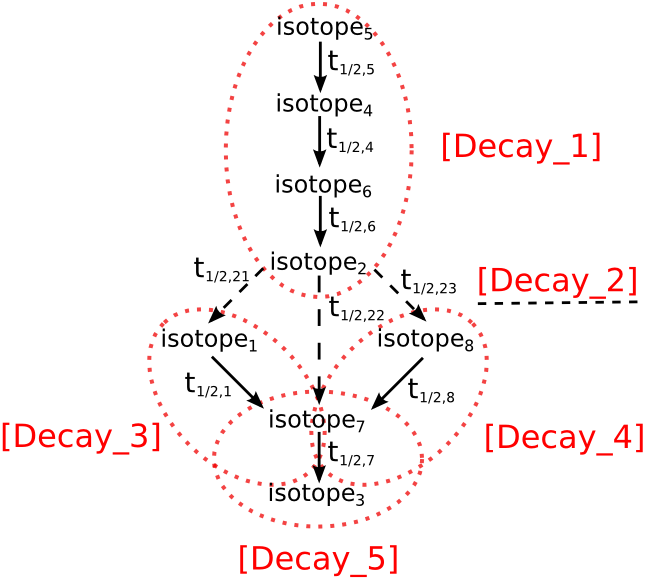
\includegraphics[width = 8cm]{\fig /decay_chain.png}
%  \caption{Decay chain with branches.}
%  \label{pic:dec_branches}
% \end{figure}
% 
% 
% When it comes to a simulation of first order reactions, the kinetic constant is given as an input. 
% The description of a kinetic chemical reaction has obviously two folowing forms
% \[
%   \begin{array}{l}
%     A\xrightarrow{k}B,\\
%     \frac{dc^A}{dt} = -k \cdot c^A.
%   \end{array}
% \]
% The first one description is a standard chemical one. The second equation describes temporal decrease in amount of concentrations of the specie $c^A$. The constant $k$ is so called kinetic constant and for the case of a first order reactions it is equal to so called reaction rate. The order of reaction with just one reactant is equal to the power of $c^A$ in partial diferential reaction.
% 
% For an inclusion of first order reaction into a reaction matrix a half-life needs to be computed from the corresponding kinetic constant $k$. The derivation follows
% \[
%   \begin{array}{l}
%     A\xrightarrow{k} B\\
%     \frac{dc^A}{d\tau} = -k\cdot c_A\\
%     \frac{dc^A}{c^A} = -k\cdot d\tau\\
%     \int\limits_{c^A_0/2}^{c^A_0}\frac{dc^A}{c^A} = -k\cdot\int\limits_{t_{1/2,A}}^{0} d\tau\\
%     \left[ ln c^A\right]_{c^A_0/2}^{c^A_0} = -[k\tau]_{t_{1/2,A}}^{0}\\
%     ln c^A_0 - \ln\frac{c^A_0}{2} = k\cdot t_{1/2,A}\\
% %     c^A (t) = c^A_0\cdot e^{-k\cdot t_{1/2,A}}\\
% %     {\bf substitution} \qquad c^A(t_{1/2,A}) = \frac{1}{2}\cdot c^A_0\\
% %     \frac{1}{2} c^A_0 = c^A_0\cdot e^{-k_1\cdot t_{1/2,A}}\\
%     \ln 2 = k \cdot t_{1/2,A}\\
%     t_{1/2,A} = \frac{ln 2}{k}
%   \end{array}                                                                                                                                                                                                                                                                                                            
% \]
% The matrix ${\bf R}$ is constructed in the same way as for the radioactive
% decay.


\subsection{Dual Porosity} 
\label{sec:num_dual_porosity}

The analytic solution of the system of differential equations \eqref{eq:odes_dual_por} at the time $t$ with initial conditions $c_m(0)$ and $c_i(0)$ is
\begin{align}
     c_m(t) &= (c_m(0) - c_a(0)) \exp\left(- D_{dp}\left(\frac{1}{\vartheta_m} + \frac{1}{\vartheta_i}\right) t \right) + c_a(0), 
     \label{eqn:dual_porosity_anal1}\\
     c_i(t) &= (c_i(0) - c_a(0)) \exp\left(- D_{dp}\left(\frac{1}{\vartheta_m} + \frac{1}{\vartheta_i}\right) t \right) + c_a(0),
     \label{eqn:dual_porosity_anal2}
\end{align}
where $c_a$ is the weighted average
\[
  c_a = \frac{\vartheta_m c_m + \vartheta_i c_i}{\vartheta_m + \vartheta_i}.
\]

If the time step is large, we use the analytic solution to compute new values of concentrations. 
Otherwise, we replace the time derivatives in \eqref{eqn:dual_porosity_ode1} and \eqref{eqn:dual_porosity_ode2} 
by first order forward differences and we get the classical Euler scheme
\begin{subequations}
\label{eq:dp_expl_euler}
\begin{align}
  c_m(t^+) = \frac{D_{dp} \Delta t}{\vartheta_m}(c_i(t) - c_m(t)) + c_m(t), \\
  c_i(t^+) = \frac{D_{dp} \Delta t}{\vartheta_i}(c_m(t) - c_i(t)) + c_i(t), \\
\end{align}
\end{subequations}
where $\Delta t = t^+ - t$ is the time step. 

The condition on the size of the time step is derived from the Taylor expansion of 
\eqref{eqn:dual_porosity_anal1} or \eqref{eqn:dual_porosity_anal2}, respectively. We neglect the higher order 
terms and we want the second order term to be smaller than the given \hyperA{DualPorosity::scheme-tolerance}{scheme tolerance} 
$tol$, relatively to $c_a$,
\begin{equation}
  (c_m(0) - c_a(0))
  \frac{ D_{dp}^2 (\Delta t)^2 \left(\frac{\vartheta_m + \vartheta_i}{\vartheta_m \vartheta_i}\right)^2}{2}
  \frac{1}{c_a} \leq tol. \\
\end{equation}
We then transform the above inequation into the following condition which is tested in the program
\begin{equation} \label{eqn:euler_scheme_condition}
  \max(|c_m(0) - c_a(0)|, |c_i(0) - c_a(0)|) \leq 
  2 c_a \left(\frac{\vartheta_m \vartheta_i}{D_{dp} \Delta t (\vartheta_m + \vartheta_i)}\right)^2 tol. \\
\end{equation}
In addition, the explicit Euler method \eqref{eq:dp_expl_euler} requires the satisfaction of a CFL condition of the form
\begin{equation}
\label{eq:dp_cfl}
\Delta t \le \frac1{D_{dp}} \frac{\th_m \th_i}{\th_m+\th_i}.
\end{equation}
If either of the inequalities \eqref{eqn:euler_scheme_condition} or \eqref{eq:dp_cfl} is not satisfied, then the analytic 
solution is used.


\subsection{Equilibrial Sorption}
\label{sec:num_sorp_math}

Let us now describe the actual computation of the sorption model.
To solve \eqref{eq:nonlin_sorption} iteratively, it is very important to define the interval where 
to look for the solution (unknown $c_l$), see Figure \ref{fig:sorpce}. The lower bound is $0$ (concentration can not reach negative values). 
The upper bound is derived using a simple mapping. Let us suppose limited 
\hyperA{Sorption::solubility}{solubility} of the selected transported substance and let us denote the 
limit $\bar{c}_l$. We keep the maximal "total mass" 
$\bar{c}_T= \mu_l\cdot \bar{c}_l + \mu_s\cdot f(\bar{c}_l)$, but we dissolve all the mass to get 
maximal $c_l^{max} > \bar{c}_l$. That means $c_s = 0$ at this moment. We can slightly enlarge the interval by setting the upper bound equal to 
$c_l^{max} + const_{small}$.

\begin{figure}[ht!]
 \centering
 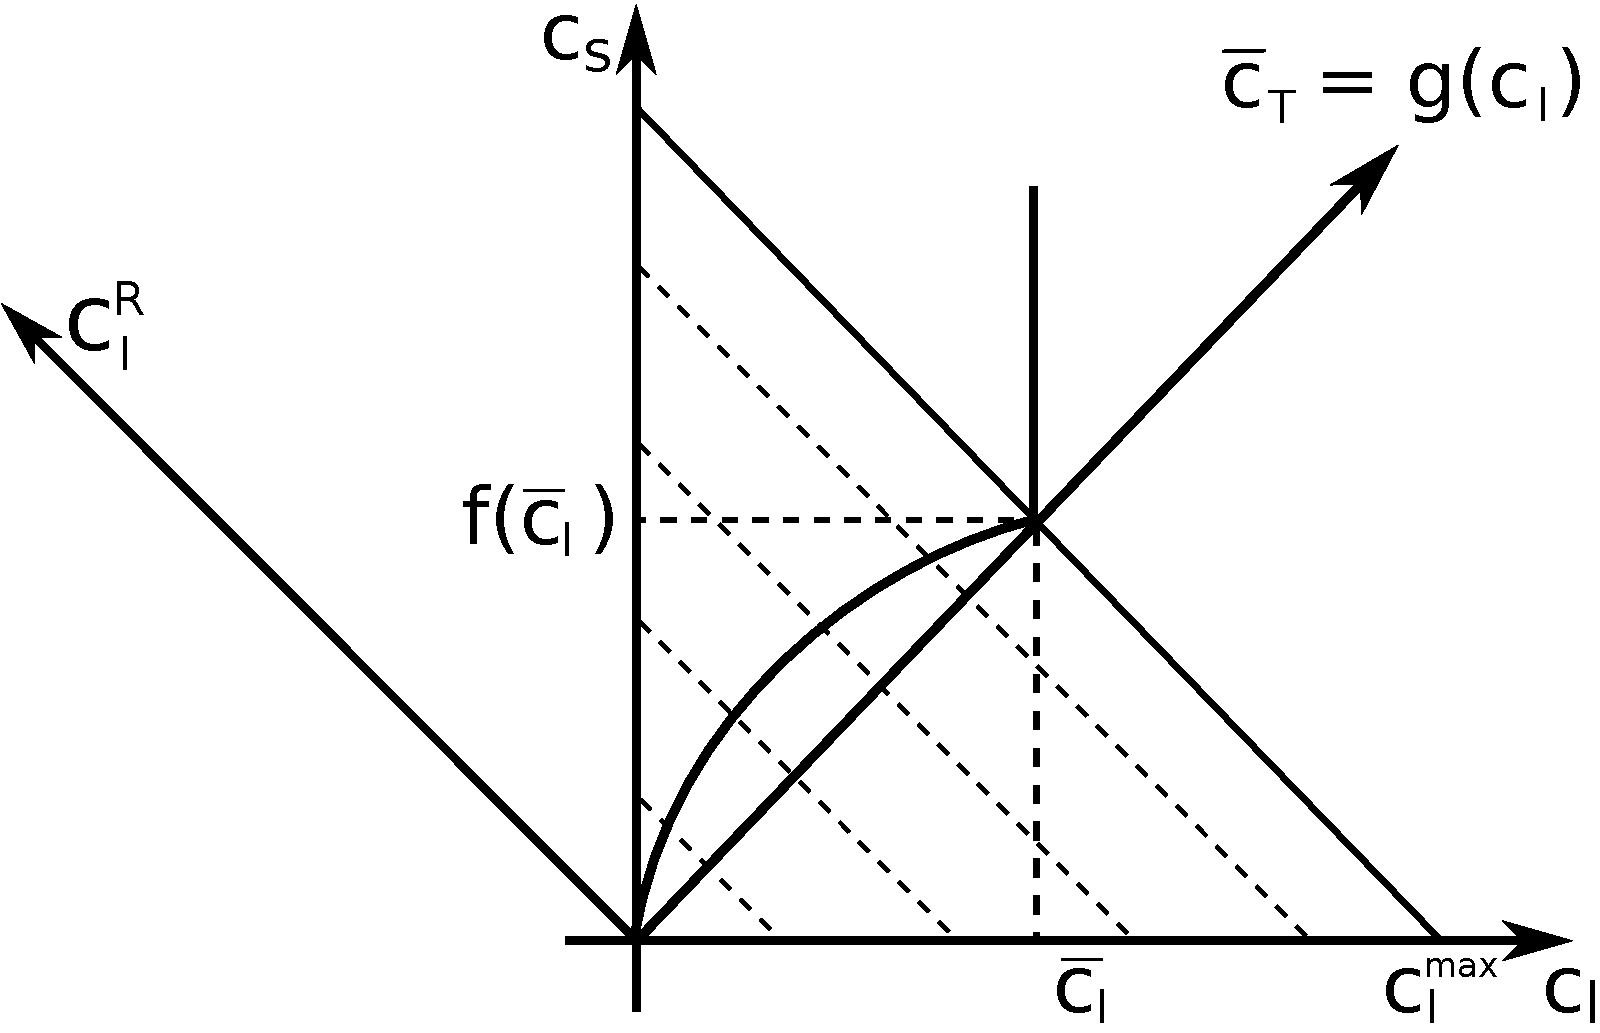
\includegraphics[width = 0.75\textwidth]{\fig/sorpce.pdf}
 \caption{Sorption in combination with limited solubility.}
 \label{fig:sorpce}
\end{figure}


To approximate the equation \eqref{eq:nonlin_sorption} using interpolation, we need to prepare the set of values 
which represents $[c_l, f(c_l)]$, with $c_l$ equidistantly distributed in transformed (rotated and rescaled) 
coordination system at first. The construction process of the interpolation table follows.
\begin{enumerate}
 \item Maximal ``total mass'' $\bar{c}_T = \mu_l\cdot \bar{c}_l + \mu_s\cdot f(\bar{c}_l)$ is computed.
 \item Total mass step is derived $mass\_step = \bar{c}_T/n\_steps$. $n\_steps$ is the number of
       \hyperA{Sorption::substeps}{substeps}.
 \item Appropriate $c_T^j = (mass\_step\cdot j)/\mu_l,~j\in \{0,\ldots, n\_steps\}$ are computed. 
 \item The equations $\mu_l \cdot c_T^j = \mu_l\cdot c_l^j + \mu_s\cdot f(c_l^j)~j\in \{0,\ldots, n\_steps\}$ are solved 
       for $c_l^j$ as unknowns. The solution is the set of ordered couples (points) 
       $[c_l^j,f(c_l^j)],~j\in\{0,\ldots,n\_steps\}$.
\end{enumerate}
After the computation of $\{[c_l^j,f(c_l^j)]\}$, we transform these coordinates to the system where the total mass is 
an independent variable. This is done by multiplication of precomputed points using the transformation matrix ${\bf A}$:
\begin{equation}
 \begin{array}{l}
  \vec{c}\,^R = {\bf A}\cdot\vec{c}\\
  \left[\begin{array}{c} c_l^{R,j}\\ c_s^{R,j} \end{array}\right] = 
  \left[\begin{array}{cc}
    \vartheta\cdot \rho_w & M_s(1 - \vartheta)\rho_R\\
    -M_s(1 - \vartheta)\rho_R & \vartheta\cdot \rho_w
  \end{array}\right]\cdot
  \left[\begin{array}{c} c_l^j\\ c_s^j \end{array}\right]\\
  j\in\{0,\ldots,n\_steps\}
 \end{array}
 \label{eq:transf_mat}
\end{equation}

The values $c_l^{R,j}$ are equidistantly distributed and there is no reason to save them, but the values 
$c_s^{R,j}$ are stored in onedimensional interpolation table.

Once we have the interpolation table, we can use it for projecting the transport results ${[c_l,c_s]}$ on the 
isotherm under consideration. Following steps must be taken.
\begin{enumerate}
 \item Achieved concentrations are transformed to the coordinate system through multiplication with the 
       matrix ${\bf A}$, see \eqref{eq:transf_mat}.
 \item Transformed values are interpolated.
 \item The result of interpolation is transformed back. The backward transformation consists of multiplication 
       with ${\bf A}^T$ which is followed by rescaling the result. Rescaling the result is necessary because  
       ${\bf A}$ is not orthonormal as it is shown bellow.
 \[
 \begin{array}{l}
 {\bf A}^T\cdot{\bf A} =
  \left((\vartheta - 1)^2\cdot M_s^2\cdot \rho_R^2 + \vartheta^2\cdot \rho_w^2\right)\cdot\left[\begin{array}{cc}
    1 & 0\\
    0 & 1
  \end{array}\right]
  \end{array}
 \]
\end{enumerate}


% \subsection{Limited Solubility}\label{subsec:lim_solub}
\paragraph{Limited solubility.} When $\mu_l\cdot c_l + \mu_s\cdot f(c_l) > \mu_l\cdot \bar{c}_l + \mu_s\cdot f(\bar{c}_l)$, neither iterative 
solver nor interpolation table is used. The aqueous concentration is set to be $\bar{c}_l$ and sorbed 
concentration is computed $c_s = (\mu_l\cdot c_l + \mu_s\cdot f(c_l) - \mu_l\cdot \bar{c}_l)/\mu_s$.

\subsection{System of Linear Ordinary Differential Equations}
\label{sec:num_slode}

A system of linear ordinary differential equations (ODE) appears in several places in the model. 
Let us denote the ODE system
\[
  \partial_t \vc c(t) = \mathbf{A}(t) \vc{c}(t) + \vc{b}(t).
\]

For the moment the only implemented method to solve the system is usage of Pad\'e approximant which corresponds to a family
of implicit R-K methods.

% \paragraph{Semi-analytic solution.}
% A semi-analytic solution can be obtained in special cases due to the physical nature of the problem.
% The problem can be then solved only by a~matrix multiplication $\vc c(t+\Delta t) = \mathbf{R} \vc{c}(t)$. 
% This is used in case of radioactive decays and first order kinetic reactions.
% 
% The right hand side $\vc{b}$ is zero and $\mathbf{A}$ is constant. The assumption is made that the equations 
% are independent during one time step. Each quantity $c_i$ (concentration in this case) is decreased 
% by $e^{a_{ii} \Delta t}$ (supposing negative diagonal) during time step $\Delta t$. The decrement $\left( 1-e^{a_{ii} \Delta t} \right)$
% is then distributed among other quantities according to the given fraction.
% 
% In case of radioactive decays and first order reactions, the elements of the solution matrix $\mathbf{R}$ are
% \begin{eqnarray*}
%      r_{ii} &=& e^{-k_i \Delta t}, \\
%      r_{ji} &=& \left( 1-e^{-k_i \Delta t} \right) b_{ji} \frac{M_j}{M_i},
% \end{eqnarray*}
% where $b_{ji}$ is the branching ratio of $i$-th reactant (or radionuclide) and $\frac{M_j}{M_i}$ is 
% the fraction of molar masses.
% The expressions $b_{ji} \frac{M_j}{M_i}$ are then obtained from the system matrix by dividing 
% $-\frac{a_{ji}}{a_{ii}}$. See the system matrix entries in \eqref{eqn:reaction_system_entries}.
% 
% The assumption (equations independence) is adequate when a very small time step is applied. This will then lead 
% to huge amount of evaluations of the exponential functions which can be expensive, so other numerical methods 
% might be more appropriate. When the time step is large then the assumption is inadequate.
% 
% On the other hand, if the time step is constant (for significantly large number of time steps), we get the
% solution cheaply just by matrix multiplication, because the matrix $\mathbf{R}$ is constant.


\paragraph{Pad{\' e} approximant.}
For homogenous systems with constant matrix $\mathbf{A}$, we can use \hyperA{IT::PadeApproximant}{Pad{\' e} approximation} 
to find the solution. This method finds a rational function whose power series agrees with a power series expansion of 
a given function to the highest possible order (e.g. in \cite{press_numerical_1992}).
Let
\[
  f(t) = \sum\limits_{j=0}^{\infty} c_j t^j = \sum\limits_{j=0}^{\infty} \frac{1}{n!}f^{(j)}(t_0)
\]
be the function being approximated and its power series given by Taylor expansion about $t_0$.
Then the rational function
\begin{equation} \label{eqn:pade_approximant}
R_{mn}(t) = \frac{P_m(t)}{Q_n(t)} = \frac{\sum\limits_{j=0}^{m} p_jt^j}{\sum\limits_{j=0}^{n} q_jt^j},
\end{equation}
which satisfies 
\begin{equation} \label{eqn:pade_coef_equations}
f(t)\approx \sum\limits_{j=0}^{m+n} c_j t^j = R_{mn}(t),
\end{equation}
% \begin{equation} \label{eqn:pade_coef_equations}
% \sum\limits_{j=0}^{m+n} c_jt^j \sum\limits_{j=0}^{m} q_jt^j = \sum\limits_{j=0}^{n} p_jt^j,
% \end{equation}
is called Pad{\' e} approximant. From \eqref{eqn:pade_coef_equations}, we obtain $m+n+2$ equations for
coefficients of the nominator $P_m$ (polynomial of \hyperA{PadeApproximant::pade-nominator-degree}{degree} $m$) and 
the denominator $Q_n$ (polynomial of \hyperA{PadeApproximant::pade-denominator-degree}{degree} $n$). We also see that the error 
of the approximation is $O(t^{m+n+1})$. By convention, the denominator is normalized such that $q_0=1$.
Theoretical results show that for $m=n-1$ and $m=n-2$ the Pad\'e approximant corresponds to an implicit Runge-Kutta method
which is A-stable and L-stable (see \cite{ehle1973}).

Now, we consider the solution of our ODE system in a form $\vc{c}(t)=e^{\mathbf{A}t}\vc{c}(0)$. We shall 
approximate the matrix exponential function using a matrix form of \eqref{eqn:pade_approximant}. 
For exponential functions, there are known coeffficients of the nominator and denominator:
% http://mathoverflow.net/questions/41226/pade-approximant-to-exponential-function
% http://www.math.vanderbilt.edu/~esaff/texts/144.pdf
% https://www-sop.inria.fr/apics/anap03/PadeTalk.pdf
\begin{eqnarray}
  \mathbf{P}_m(\mathbf{A}t) &=& \sum\limits^{m}_{j=0}\frac{(m+n-j)!m!}{(m+n)!j!(m-j)!} (\mathbf{A}t)^j, \\
  \mathbf{Q}_n(\mathbf{A}t) &=& \sum\limits^{n}_{j=0} (-1)^j \frac{(m+n-j)!n!}{(m+n)!j!(n-j)!} (\mathbf{A}t)^j.
\end{eqnarray}
Finally, we can write the solution at time $t+\Delta t$
\begin{equation} \label{eqn:pade_solution}
\vc{c}(t+\Delta t) = \frac{\mathbf{P}_m(\mathbf{A}\Delta t)} {\mathbf{Q}_n(\mathbf{A}\Delta t)}\vc{c}(t) 
= \mathbf{R}_{mn}(\mathbf{A}\Delta t)\vc{c}(t).
\end{equation}

If the time step $\Delta t$ is constant, we do not need to compute the matrix $\mathbf{R}_{mn}$ repeatedly and we get
the solution cheaply just by matrix multiplication. In the oposite case, we avoid evaluating the exponential
function and still get the solution quite fast (comparing to computing semi-analytic solution).

%\subsection{General Chemical Reactions}
For a simulation of general chemical reactions as a part of reactive transport simulation, an application Semchem has been merged together with Flow123D. It enables to simulate following types of reactions:
\begin{itemize}
  \item Chemical equilibrium (solved using iterative Newtons method)
    \subitem mathematical description $K^{(r)} = \prod_i c_i^{\alpha_i^{(r)}},$

  \item Slow evolving chemical kinetics (solved using Runge-Kutta method)
    \subitem mathematical description $\frac{dc_i}{dt} = -k^{(r)}\prod_j c_j^{\beta_j^{(r)}},$

  \item Fast evolving chemical kinetics (discretized using implicit Eulerova method and solved using Newtons method)
     \subitem mathematical description $\frac{c_i^{(T+1)} - c_i^{T}}{\Delta t} = -k^{(r)}\prod_j c_j^{\beta_j^{(r),(T+1)}},$
  \item Radioactive decay can be simulated as a special case of first order reaction.
\end{itemize}

Further informations can be found in ``Snizeni poctu nelinearnich rovnic popisujicich chemicke reakce''.


\chapter{File Formats}
\label{chapter:file-formats}
%\section{Input format}


\chapter{New input files}
The input consists of the root input file given as the parameter on the command line and possibly several other 
files with large input data. In this section we shall describe format of the input files. At first, we specify syntax of
an extension to the JSON file format. Then we set rules for input of more specific data constructs. We continue by description of general scheme for input of
boundary conditions and material time-space variable data. And finally, we describe setting of particular equations and their solvers.

The aim of this draft is twofold. First, we want to outline the way how to translate current input file format (in version 1.6.5) into the new one without extending 
the existing functionality. Second, we want to propose a new way how to input general boundary and material data. Desired features are:
\begin{itemize}
 \item input simple data in simple way
 \item possibility to express very complex input data 
 \item possibility to generate data automatically, and input very large input sets
 \item input interface that provides uniform access to the data in program independent of the input format
\end{itemize}
[ ... something else?]

As this is a draft version there are lot of remarks, suggestions and questions in square brackets. Some keys are marked OBSOLETE, which means that 
we want to replace them by something else.

\section{Root file format}
The root input file is in the Humanized JSON file format. That is the JSON file format with few syntax extensions and several semantic rules particular to
Flow123d. The syntax extensions are
\begin{enumerate}
\item You can use one line comments using hash \verb'#'.
\item The quoting of the keys is optional if they do not contain spaces (holds for all Flow keys).
\item You can use equality sign \verb'=' instead of colon \verb':' for separation of keys and values in JSON objects.
\item You can use any whitespace to separate tokens in JSON object or JSON array.
\end{enumerate}
The aim of these extensions is to simplify writing input files manually. However these extensions can be easily filtered out and converted to 
the generic JSON format. (This way it can be also implemented in Flow123d.)

For those who are not familiar with the JSON file format, we give the brief description right here. The full description can be found at
\url{http://www.json.org/}. However, we use term {\it record} in the place of the {\it JSON object} in order to distinguish {\it JSON object}, 
which is merely a data structure written in the text, and the {\it C++ object}, i.e. instance of some class. 

\subsection{Humanized JSON}
The JSON format consists of four kind of basic entities: 
{\it null} token, {\it true} and {\it false} tokens, {\it number}, {\it string}. {\it Number} is either integer or float point number 
possibly in the exponential form and {\it string} is any sequence of characters quoted in \verb'""' (backslash \verb"\" is used as escape character and 
Unicode is supported, see full specification for details). 

In the following, we mean by white space characters:
space, tab, and new line. In particular the newline character (outside of comment or quoting) is just the white space character without any special meaning.

The basic entities can be combined in composed entities, in a {\it record} or in an {\it array}. The {\it record} is set of assignments enclosed in the curly brackets
\begin{verbatim}
{
        #basic syntax
        "some_number":124, 
        "some_string":"Hallo",
        "some_subrecord":{},
        "some_array":[],
        
        #extended syntax
        non_quoted_key_extension=123,
        separation_by_whitespace="a" sbw_1="b"
        sbw_2="c"
}
\end{verbatim}
One assignment is a pair of the {\it key} and the {\it value}. {\it Key} is {\it string} or token matching regexp\\
\verb'[a-zA-Z_][a-zA-Z_0-9]*'.
{\it Value} is basic or composed entity.
The key and the value are separated by the colon (generic syntax) or equality sign (extended syntax). Pairs are separated by a comma (generic syntax) or 
sequence of white space characters (extended syntax). The values stored in the record are accessed through the keys like in an associative array. Records are usually used for initialization of corresponding classes.

The second composed entity is the {\it array} which is sequence of (basic or composed) entities separated by comma (generic syntax) or whitespace sequence 
(extended syntax) and enclosed in the square brackets. 
The values stored in the array are accessed through the order. The Flow reader offers either initialization of a container from JSON array or
a sequential access. The latter one is the only possible access for the included arrays, which we discuss later.

On any place out of the quoted string you can use hash mark \verb'#' 
to start a one line comment. Everything up to the new line will be ignored and replaced by single white space.

[What about multiple line strings? (Should be allowed)]

\subsection{Special keys}
Apart from small extensions of JSON syntax, we impose further general rules on the interpretation of the input files by Flow123d reader.
First, the capital only keywords  
have a special meaning for Flow JSON reader. On the other hand, we use only small caps for keys interpreted through the reader.
The special keywords are:
\begin{description}

\item[TYPE]:\\ 
\begin{verbatim}
TYPE= <enum>
\end{verbatim}
The \verb'<enum>' is particular semantic construct described later on. 
When appears in the record, it specifies which particular class to instantiate. This only has meaning if the record initializes
an abstract class. In consistency with the source code, we shall call such records {\it polymorphic}. 


In fact we consider
that every record is of some {\it type} at least implicitly. The {\it type} of the record is specification of the keys that are
interpreted by the program Flow123d. At some places the program assumes a record of specific {\it type} so you need not to specify 
\verb'TYPE' key in those records.

\item[INCLUDE\_RECORD]:\\
This is a simple inclusion of another file as a content of a record:
\begin{verbatim}
{
        INCLUDE_RECORD = "<file name>"
}
\end{verbatim}

\item[INCLUDE\_ARRAY]:\\
\begin{verbatim}
array=
{
        INCLUDE_ARRAY = "<file name>"
        FORMAT = "<format string>"
}       
\end{verbatim}
The reader will substitute the include record by a sequentially accessible array. The file has fixed number of 
space separated data fields on every line. Every line becomes one element in the array of type record. Every line forms a 
record with key names given by the \verb'<format string>' 
and corresponding data taken form the line.

The key difference compared to regular JSON arrays is that included arrays can be accessed only sequentially 
within the program and thus we minimize reader memory overhead for large input data. The idea is to translate raw data into structured
format and use uniform access to the data.

Basic syntax for format string could be an array of strings --- formats of individual columns.
Every format string is an address of key that is given the column. Onother possibility is to give an arbitrary 
JSON file, where all values are numbers of columns where to take the value.

[\dots better specify format string]


[Possible extensions:
- have sections in the file for setting time dependent data
- have number of lines at the beginning
- have variable format
- allow vectors in the 'line records']

\item[REFERENCE]:\\
\begin{verbatim}
time_governor={
  REF=<address>
}
\end{verbatim}
This will set key \verb'time_governor' to the same value as the entity specified by the address.
The address is an array of strings for keys and integers for indices.
The address can be absolute or relative identification of an entity. The relative address is relative to the entity in which the reference record is contained.
One can use string \verb'".."' to move to parent entity and string \verb'"//"' to move to the root record of current file.
Indices in address starts from 0.

For example assume the file
\begin{verbatim}
mesh={
        file_name="xyz"
}
array=[
        {x=1, y=0}       
        {x=2, y=0}
        {x=3, y=0}
]               
outer_record={
        output_file="x_out"
        inner_record={
                output_file={REF=["..","output_file"]}  # value "x_out"
        }
        x={REF="/array/2/x"}                                    # value "3"
        f_name={REF=["//","mesh","file_name"]}                  # value "xyz"
}       
\end{verbatim}

Concept of addres should be better explained and used consistently in reader interface.
\end{description}

\subsection{Semantic rules}

\subsubsection{Implicit creation of composed entities}
Consider that there is a {\it type} of record in which all keys have default values (possibly except one). Then the specification
of the record {\it type} can contain a {\it default key}. Then user can use the value of the {\it default key} instead of the whole record.
All other keys apart from the {\it default key} will be initialized by default values. 
This allows to express simple tasks by simple inputs but still make complex inputs possible. 
In order to make this working, developers should provide default values everywhere it is possible.
 
Similar functionality holds for arrays. If the user sets a non-array value where an array is expected the reader provides an array with a unique element holding the given value.
See examples in the next section for application of these two rules.



\subsubsection{Enum construct}
Enum values can be integers or strings from particular set. Strings should be preferred for manual creating of input files, while 
the integer constants are suitable for automatic data preparation. 

The input reader provides a way how to define names of members of an enum class and then 
initialize this enum class from input file.  [Need better description]

\subsubsection{String types}
For purpose of this documentation we distinguish several string types with particular purpose and treatment. Those are:
\begin{description}
\item[input filename] This has to be valid absolute or relative path to an existing file. 
The string can contain variable \verb'${INPUT}' %$
which will be replaced by path given at command line through parameter \verb'-i'.

[In order to allow input of  time dependent data in individual files, we should 
 have also variable \verb'${TIME\_LEVEL}' %$
 From user point of view this is not property of general input filename string, however
 in implementation this should be done in the same way as \verb'${INPUT}'.
]
 
[? Shall we allow both Windows and UNIX slashes?]

[Developers should provide default names to all files. ]

\item[output filename] This has to be relative path. The path will be prefixed by
the path given at command line through the parameter \verb'-o'.
In some cases the path will be also postfixed by extension of particular file format.

\item[formula] Expression that will be parsed and evaluated runtime. Documentation of particular key should provide 
variables which can appear in the expression, however in general it can be function of the space coordinates $x$, $y$, $z$ and possibly also 
function of time $t$. For full specification of expression syntax see documentation of FParser library:
\url{http://warp.povusers.org/FunctionParser/fparser.html\#literals}

\item[text string] Just text without particular meaning.
\end{description}

\subsubsection{Record types}
A record type like particular definition of a class (e.g. in C++). One record type serves usually for initialization of 
one particular class. From this point of view one record type is set of keys that corresponding class can read.

For purpose of this manual the record type is given by specification of record's keys, their types, default values and meanings.
In the next two sections, we describe all record types that forms input capabilities of Flow123d. Description of a record type 
has form of table. Table heading consists of the name of the record type. Then for every key we present name, type of the value,
default value and text description of key meaning. Type of the value can be record type, array of record types, double, integer, enum or 
string type. Default value specification can be:
\begin{description} 
 \item[none] No default value given, but input is mandatory. You get an error if you don't set this key.
 \item[null] \verb'null' value. No particular default value, but you need not to set the key. Usually means feature turned off.
 \item[explicit value] For keys of type: string, double, integer, or enum, the default value is explicit value of this type.
 \item[type defaults] For keys of some record type we let that record to set its default values.
\end{description}

[? polymorphic record types]


\section{Record types for input of data fields}


\newenvironment{recordtype}[2]
{\par
 \vskip 2ex
 \noindent%
 record type: {\bf #1}#2
 \par%
 \vskip 0.5ex
 \hrule%
 \vskip 0.3ex
 \hrule
 \begingroup%records of steady field type which we describe right now 
  \addtolength{\leftskip}{3em}%
  %
  \gdef\keyitem##1##2##3{%
    \par
    \vskip 0.3ex
    %\hrule%
    \noindent%
    \hspace{-3em}{\bf\tt ##1} = {\it \textless ##2\textgreater} \hfill \makebox[0.4\textwidth][l]{DEFAULT: {##3}\hfil}%
    \par
  }%
}{%
  \vskip 0.7ex  
  \hrule%
  \vskip 0.5ex
  \endgroup%
}

\def\enumhead#1{
{\bf #1} enum cases:
}
\def\enumitem#1#2{
  \par{\tt #1=#2 \hspace{2em}}
}

In this section we describe record types used to describe general time-space scalar, vector, or tensor fields
and records for prescription of boundary conditions. Since one possibility how to prescribe input data fields is by 
discrete function spaces on computational mesh, we begin with mesh setting.

\subsection{Mesh type}
The mesh record and should provide a mesh consisting of points, lines, triangles and tetrahedrons in 3D space and further
definition of boundary segments and element connectivity.

\begin{recordtype}{Mesh}{}

\keyitem{file}{input filename}{mesh.msh}
The file with computational mesh in the ASCII GMSH format.\\
\url{http://geuz.org/gmsh/doc/texinfo/gmsh.html#MSH-ASCII-file-format}

\keyitem{boundary\_segments}{array of boundary segments}{null optional}
The set of 0,1, or 2 dimensional boundary faces of the mesh should be partitioned into boundary segments in order to prescribe unique boundary condition 
on every boundary face. 
The segments numbers are assigned to boundary faces by iterating through the array. Initially every boundary face has segment number $0$. 
Every record in the array use ``auxiliary'' physical domains, elements or direct face specification to specify some set of boundary faces. The new segment number
is assigned to each face in the set, possibly overwriting previous value.

Physical domains or its parts that appears in the boundary segment definitions are removed form the computational mesh, however, the element
numbers of removed elements are stored in the corresponding boundary face and can be used to define face-wise approximations of functions with 
support on the boundary.

\keyitem{neighbouring}{input file name}{neigbours.flw}
This should be removed as soon as we integrate ngh functionality into flow.
\end{recordtype}

\begin{recordtype}{Boundary segment}{}
 \keyitem{index}{integer}{index in outer array}
 The index of boundary segment can be used later to prescribe particular type of boundary condition on it.
 Indices must be greater or equal to $1$ and should form more or less continuous sequence. The zero boundary segment is reserved for remaining part
 of the boundary. By default we assign indices to boundary segments according to the order in their array in mesh, i.e. index (counted form $0$) plus $1$.
 \keyitem{physical\_domains}{array of integers}{null optional}
 Numbers of physical domains which form the boundary segment. All elements of these physical domains will be removed from actual computational mesh.
 \keyitem{elements}{array of integers}{null optional}
 The array contains element numbers which should be removed from computational mesh and added to boundary segment.
 \keyitem{sides}{array of integer pairs}{null optional}
 The array contains numbers of elements which outer faces will be added to the boundary segment or pairs $[element, side\_on\   _element]$ 
 identifying individual faces that will be added to the boundary segment.
\end{recordtype}

\subsection{Time-space field type}
A general time and space dependent, scalar, vector, or  tensor valued function is given by array
of {\it steady field data}, i.e. time slices. The time slice contains array of {\it space functions}
for individual materials. Then, the {\it space function} can by either analytical (given by formula)
or numerical, given by type of discrete space and array of {\it elemental functions}. {\it Elemental function} is
just array of values for every degree of freedom on one element.

The function described by this type is tensor values in general and dimensions of this tensor should be 
specified outside of the function data. For example in description of Transport record type you should specify that function
for initial condition is vector valued with vector size equal to number of substances. It is like template for Time-space field
type parametrized by shape of the value tensor given by number of lines $N$ and columnes $N$.


\begin{recordtype}{Steady field data}{}
\keyitem{time}{double}{-Inf}
  Start time for the spatial filed data. 
\keyitem{time\_interpolation}{enum}{constant}
  \enumhead{time interpolation}
  \enumitem{constant}{0} Keeps constant data until next time cut.
  \enumitem{linear}{1} Linear interpolation between current time cut and the next one.
\keyitem{materials}{array of Steady spatial functions}{null optional}
\end{recordtype}

\begin{recordtype}{Space function}{}
\keyitem{material}{integer}{0}
Material filter. The function has nonzero value only on elements with given material number. 
Function with filter $0$ takes place for all materials where no function is set.

\keyitem{analytic}{multi-array of function formulas}{null optional}
The shape of the multi-array is given by 
rank of the value of the function. Since formula parser can deal only with scalar functions, we
have to specify individual members of resulting tensor. Formulas can contain variables $x$, $y$, $z$, and $t$. 
The formula is used until the next time slice and is evaluated for every solved time step (can depend on equation).

Instead of constant formulas one can use double values.
Usage of formulas or doubles need not to be uniform over the tensor.


\keyitem{numeric\_type}{enum}{None}
  \enumhead{FE space}
  \enumitem{None}{0} Use analytic function.
  \enumitem{P0}{1} Zero order polynomial on element.

Currently we support only P0 base functions for data.

\keyitem{numeric}{array of element functions}{empty array}
Usually, this element-wise array should by included from an external file through \verb'INCLUDE_ARRAY' construct.

\end{recordtype}

\begin{recordtype}{Element function}{}
\keyitem{element\_id}{integer}{null optional}
Element ID in the mesh. By default the element is 
identified by the index in the array of element function.

\keyitem{values}{multi-array of doubles}{null mandatory}
Values for degrees of freedom of the base functions on the element. Currently we support 
only P0 functions which are given by value in the barycenter of the element. 
In general the value can be tensor, i.e. array of arrays of doubles.
However, in accordance to simplification rules, you can use only array of doubles for 
vector functions or mere double for scalar functions.
\end{recordtype}

[ tensor/vector valued element function should be given also as simple array of DOF values. But
  we have to provide ordering of tensor products of FE spaces]

[ As follows from next examples, there is no way how to simply set simply tensors.  We can introduce automatic conversion form scalar to  vector (constant vector) and vector to tensor 
(diagonal tensor). ]

[ we should also allow 'in place' array includes to simplify material tables etc.]

[How to allow parallel input of field data?]

[Should be there explicit mesh reference in the field specification?]


Examples:
\begin{verbatim}
constant_scalar_function = 1.0
# is same as
constant_scalar_function = {
  time = -Inf,
  time_interpolation= constant,
  materials = [
    {
      rank=0
      numeric_type=None
      analytic=1.0       # the only key withou default value
    }
  ]
}

conductivity_tensor = 
  [{ material = 1,
     rank = 2,
     analytic = [[1.0, 0.0, 0.0], [0.0, 1.0, 0.0], [0.0, 0.0, 1.0]]
   },
   { material = 2,
     rank = 2,
     analytic = [[10.0, 0.0, 0.0], [0.0, 10.0, 0.0], [0.0, 0.0, 10.0]]
   }
  ]
 
\end{verbatim}

\subsection{Boundary conditions}
Input of boundary conditions is similar to the Time-space fields. For description of one time slice we have 
type {\it steady boundary data}. This contains array of {\it boundary conditions} for individual boundary segments. 
{\it Boundary condition} is given by type and parameters that are analytic or numeric functions. However, numeric functions
are considered only on boundary elements.

\begin{recordtype}{steady boundary data}{}
\keyitem{time}{double}{0.0}
Time when the BC should be applied.
\keyitem{bc}{array of boundary conditions}{empty} 
\end{recordtype}

\begin{recordtype}{boundary condition}{}
 \keyitem{boundary\_segment}{integer}{0}
  Boundary segment where the boundary condition will be applied.
 \keyitem{bc\_type}{enum}{dirichlet}
  Currently there are just three types of boundary condition common to all equations, 
  but some equations can implement some specific boundary conditions. Common boundary condition  types are
  \enumhead{BC types}
  \enumitem{dirichlet}{0}
  \enumitem{neumann}{1}
  \enumitem{newton}{2} (also known as Robin boundary condition)


\keyitem{value}{space function}{type defaults}
Prescribed value for Dirichlet boundary condition and Newton boundary condition, the normal flux for the Neumann boundary condition.
Key \verb'material' of {\it space function} is irrelevant.

\keyitem{mean\_value}{scalar or vector constant}{0}
Prescribes flux for Neumann boundary condition by total flux over the boundary segment. If both {\it value} and {\it mean\_value} keys
are set, we use only {\it value} key. 
[How this interact with fracture opening?]


\keyitem{newton\_coef}{scalar space function}{type defaults}
Coefficient that appears in the Newton boundary condition. Key \verb'material' of {\it space function} is irrelevant.
\end{recordtype}

E.g. denoting $u$ the unknown scalar or vector field and $\prtl_n u$ density of the normal flux of this field,
the meaning of keys \verb'value' and \verb'newton_coef' is following:
$\vc{v}$ $\grad v$
\begin{align*}
 u &:= value &&\text{for Dirichlet boundary} \\
 A\grad u \cdot \vc{n} &:= value && \text{for Neumann  boundary} \\
A\grad u \cdot \vc{n} &:= newton_coef ( u - value ) && \text{for Newton boundary}
\end{align*}

Specific interpretation of the boundary conditions should be described in particular equations.

[How to allow both analytic  and numerical functions here?]

[ In order to allow changing BC type in time, the structure has to be: time array of BC segments array of BC type with data
alternatively we can have just one array of BC patches, where one patch has: time, BC segment, BC type, BC data
patches with non monotone time will be scratched]

[need vector valued Dirichlet (and Neuman, and Newton) for Transport boundary conditions]

[More examples...]


\section{Other record types recognized by Flow123d}

\subsection{Record types not related to equations}

\begin{recordtype}{Root record}{}
  \keyitem{system}{system type}{type defaults}
  Record with application setting.
  \keyitem{problem}{problem type}{null mandatory}
  Record with numerical problem to solve. 
  \keyitem{material}{input filename}{material.flw}
    Old material file still used for initialization of data fields in equations. 
    This should be replaced by material database type. Then certain input data fields in equations can be 
    constructed from material informations. Main obstacle are various adsorption algorithms depending on material number.
\end{recordtype}

Only these  keys are recognized directly at main level, however you can put here your own keys and then reference
to them. For example \verb'mesh' is part of problem type record, but you can put it on the main level and use reference 
inside \verb'problem'. 

[Should we put problem record to the main level?]

[Should we provide ``material database''? Possibility to specify properties of individual materials and use them to construct
 field data for equations.]

\begin{recordtype}{System}{}
\keyitem{pause\_after\_run}{bool}{no}
Wait for press of Enter after run. Good for Windows users, but dangerous for batch computations. 
Should be rather an command-line option.
\keyitem{verbosity}{bool}{no}
Turns on/off more verbose mode. 
\keyitem{output\_streams}{output stream}{null optional}
One or more output data streams.
There are two predefined output streams:


vtk ascii stream:
\begin{verbatim}
{
  name="dafault_vtk_ascii"
  file="flow_output"
  type="vtk_ascii"
}
\end{verbatim}

GMSH ascii stream:
\begin{verbatim}
{
  name="dafault_gmsh_ascii"
  file="flow_output"
  type="gmsh_ascii"
}
\end{verbatim}

\end{recordtype}

Possibly here could be variables for check-pointing, debugging, timers etc.

\begin{recordtype}{Output stream}{}
 \keyitem{name}{string}{null mandatory}
  Name of the output stream. This is used to set output stream for 
  individual output data. 
 \keyitem{file}{output filename string}{stream name}
  File name of the output file for the stream. The file name should be without extension, the correct extension
  will be appended according to the format type.
 \keyitem{format}{enum}{vtk\_ascii}
   \enumhead{output format}
   \enumitem{vtk\_ascii}{0} 
   \enumitem{gmsh\_ascii}{1}
 \keyitem{precision}{integer}{8}
 Number of valid decadic digits to output floating point data into the ascii file formats.
 \keyitem{copy\_file}{output filename string}{null optional}
 Optionally one can set copy file to output data into to different file formats.
 \keyitem{copy\_format}{enum}{null optional}
 \keyitem{copy\_precision}{integer}{8}
\end{recordtype}


\subsection{Equation related record types}
Up to now there is only one problem type: \verb'TYPE=sequential\_coupling', 
but in near future we should introduce full coupling e.g. for density driven flow.

The {\emph sequential coupling problem} has following keys:
\begin{recordtype}{Sequential coupling}{ implements {\it Problem type} }
\keyitem{description}{string}{null optional}
Short text description of solved problem. Now it is only reported on the screen, but could be 
written into output files or used somewhere else.
%
\keyitem{mesh}{mesh type}{type defaults}
The computational mesh common for both coupled equations.
%
\keyitem{time\_governor}{time governor type}{type defaults}
Common time governor  setting.
[ Future: allow different setting for each equation]
%
\keyitem{primary\_equation}{darcy flow type}{type defaults}
Independent equation.
%
\keyitem{secondary\_equation}{transport type}{null optional}
Equation with some data dependent on the primary equation.
\end{recordtype}

\begin{recordtype}{Time governor}{}
\keyitem{init\_time}{double}{0.0}
Time when an equation starts its simulation.
\keyitem{time\_step}{double}{1.0}
Initial time step.
\keyitem{end\_time}{double}{1.0}
End time for an equation. 
\end{recordtype}

This record type should initialize \verb'TimeGovernor' class, but there are still questions about steady TimeGovernor and 
if we allow user setting for other parameters.

There are three subtypes {\it steady saturated MH}, {\it unsteady saturated MH}, {\it unsteady saturated LMH}
The common keys are:

\begin{recordtype}{Darcy flow}{(abstract type)}
\keyitem{TYPE}{enum}{}
  There are three implementations of Darcy flow. Most keys are common but unsteady solvers accept some extra keys.
  \enumhead{darcy flow type}
  \enumitem{steady\_MH}{0}
  \enumitem{unsteady\_LMH}{1}
  \enumitem{unsteady\_MH}{2}
\keyitem{sources}{time-space field}{0} Density of water sources. Scalar valued field (1x1 tensor).
\keyitem{sources\_file}{input file name}{null optional}
File with sources in old format. (OBSOLETE)
%
\keyitem{coef\_tensor}{tensor steady field}{1.0}
Conductivity 3x3 tensor. [Should be always 3x3 and then restricted on 2d and 1d fractures.]
\keyitem{boundary\_condition}{array of steady boundary data}{null mandatory} 
New scheme for setting boundary conditions.
\keyitem{boundary\_file}{input file name}{null mandatory}
File with boundary conditions in old format. (OBSOLETE)
%
\keyitem{solver}{solver type}{type defaults}
\keyitem{n\_schurs}{integer}{2}
Number of Schur complements to make. Valid values are 0,1,2.
%
\keyitem{output}{darcy flow output type}{typ defaults}
This is just sub record to separate output setting. 
%
\keyitem{initial}{steady data type}{null mandatory}
Initial condition. Scalar valued field (1x1 tensor). (for unsteady only)
\keyitem{initial\_file}{input file name}{null mandatory}
File with initial condition in old format. (OBSOLETE)
%
\keyitem{storativity}{steady data type}{null mandatory}   
Storativity coefficient. Scalar valued field (1x1 tensor). (for unsteady only)
\end{recordtype}

\begin{recordtype}{Darcy flow output}{}
\keyitem{save\_step}{double}{null optional}
Time step between outputs.
\keyitem{output\_times}{array of doubles}{null optional}
Force output in prescribed times. Can be combined with regular otuptu given by \verb'save_step'.
\keyitem{velocity\_p0}{output stream name}{default\_vtk\_ascii}
\keyitem{pressure\_p0}{output stream name}{default\_vtk\_ascii}
\keyitem{pressure\_p1}{output stream name}{default\_vtk\_ascii} 
\end{recordtype}
 


\subsection{Solver type}
\begin{recordtype}{Solver type}{ (abstract)}
 \keyitem{TYPE}{enum}{petsc}
 \enumhead{solver types}
 \enumitem{petsc}{0} Use any PETSc solver for MPIAIJ matrices.
 \enumitem{bddc}{1} Use BDDC solver (need not to work with every equation).
 %
 \keyitem{accuracy}{double}{solvers defaults}
 Absolute residual tolerance. 
 \keyitem{max\_it}{integer}{1000}
 Maximum number of outer iterations.
 \keyitem{parameters}{string}{null optional}
 String with options for PETSc solvers.
 \keyitem{export\_to\_matlab}{bool}{no}
 Save every solved system in matlab format. Useful for debugging and numerical experiments.
 %
\end{recordtype}


\subsection{Transport type}
\begin{recordtype}{Transport type}{}
 \keyitem{sorption}{bool}{no}
 \keyitem{dual\_porosity}{bool}{no}
 \keyitem{transport\_reactions}{bool}{no}
 What kind of reactions is this? Age of water?
 %
 \keyitem{reactions}{reaction type}{null optional}
 Currently only Semchem is supported. [Interface to Phreaq ...]
 \keyitem{decays}{array of decays}{null optional}
 \keyitem{substances}{array of strings}{null mandatory}
 Names for transported substances. Number of substances is given implicitly by size of the array.
 %
 \keyitem{initial}{steady data type}{null mandatory}
 Vector valued initial condition for mobile phase of all species. 
 \keyitem{initial\_others}{steady data type}{null optional}
 Tensor valued initial condition for immobile, mobile-sorbed, immobile-sorbed phases and all species. (3 x n\_substances).
 [alternatively have separate key for each phase]
 \keyitem{initial\_file}{input file name}{null mandatory}
 File with initial condition in old format. (OBSOLETE)
 %
 \keyitem{boundary\_condition}{array of steady boundary data}{null mandatory} 
 New scheme for setting boundary conditions.
 \keyitem{boundary\_file}{input file name}{null mandatory}
 File with boundary condition in old format. (OBSOLETE)
 For time dependent boundary conditions, the filename is postfixed with 
 number of time level.
 \keyitem{bc\_times}{array of doubles}{null optional}
  Times for changing boundary conditions. If you set this variable, you have to prepare a separate file with boundary conditions for every 
  time in the list. Filenames for individual time level are formed from BC filename by appending underscore and three digits of time level number, e.g. 
  {\tt transport\_bcd\_000, transport\_bcd\_001, etc.} (OBSOLETE)
 \keyitem{output}{transport output}{type defaults}  

\end{recordtype}

\begin{recordtype}{Transport output}{}
\keyitem{save\_step}{double}{null optional}
Time step between outputs.
\keyitem{output\_times}{array of doubles}{null optional}
Force output in prescribed times. Can be combined with regular otuptu given by \verb'save_step'.
\keyitem{mobile\_p0}{output stream name}{default\_vtk\_ascii}
\keyitem{immobile\_p0}{output stream name}{default\_vtk\_ascii}
\keyitem{mobile\_sorbed\_p0}{output stream name}{default\_vtk\_ascii} 
\keyitem{immobile\_sorbed\_p0}{output stream name}{default\_vtk\_ascii} 
\keyitem{mobile\_p1}{output stream name}{default\_vtk\_ascii}
\keyitem{immobile\_p1}{output stream name}{default\_vtk\_ascii}
\keyitem{mobile\_sorbed\_p1}{output stream name}{default\_vtk\_ascii} 
\keyitem{immobile\_sorbed\_p1}{output stream name}{default\_vtk\_ascii} 
\end{recordtype}

\begin{recordtype}{Reaction}{}
% \key{Output\_precission} & \type{int} & 1 &
%Number of decimal places written to output file created by Semchem\_module.
%\\
%\hline
%\key{Number\_of\_further\_species} & \type{int} & 0 &
%Concentrations of these species are not computed, because they are ment to be unexghaustible.
%\\
%\hline
%\key{Temperature} & \type{double} & 0.0 &
%Temperature, one of state variables of the system.
%\\
%\hline
%\key{Temperature\_Gf} & \type{double} & 0.0 &
%Temperature at which Free Gibbs Energy is specified.
%\\
%\hline
%\key{Param\_Afi} & \type{double} & 0.0 &
%Parameter of the Debuy-H\"{u}ckel equation for activity coeficients computation.
%\\
%\hline
%\key{Param\_b} & \type{double} & 0.0 &
%Parameter of the Debuy-H\"{u}ckel equation for activity coeficients computation.
%\\
%\hline
%\key{Epsilon} & \type{double} & 0.0 &
%Epsilon specifies relative norm of residuum estimate to stop numerical algorithms used by Semchem\_module.
%\\
%\hline
%\key{Time\_steps} & \type{int} & 1 &
%Number of transport step subdivisions for Semchem\_module.
%\\
%\hline
%\key{Slow\_kinetics\_substeps} & \type{int} & 0 &
%Number of substeps performed by Runge-Kutta method used for slow kinetics simulation.
%\\
%\hline\\
%\key{Error\_norm\_type} & \type{string} & "Absolute" &
%Through wich kind of norm the error is measured.
%\\
%\hline\\
%\key{Scalling} & \type{boolean} & "No" &
%Type of the problem preconditioning for better convergence of numerical method.
%\\
%\hline\\
%\end{initable}
%\newpage
%\begin{initable}{Aqueous\_species}
%\key{El\_charge} & \type{int} & 0 &
%Electric charge of an Aqueous\_specie particleunder consideration.
%\\
%\hline
%\key{dGf} & \type{double} & 0.0 &
%Free Gibbs Energy valid for TemperatureGf.
%\\
%\hline
%\key{dHf} & \type{double} & 0.0 &
%Enthalpy
%\\
%\hline
%\key{Molar\_mass} & \type{double} & 0.0 &
%Molar mass of Aqueous\_species.
%\\
%\hline
%\end{initable}
%
%\begin{initable}{Further\_species}
%\key{Specie\_name} & \type{string} & "" &
%Name belonging to Further\_specie under consideration.
%\\
%\hline
%\key{dGf} & \type{double} & 0.0 &
%Free Gibbs Energy valid for TemperatureGf.
%\\
%\hline
%\key{dHf} & \type{double} & 0.0 &
%Enthalpy
%\\
%\hline
%\key{Molar\_mass} & \type{double} & 0.0 &
%Molar mass of Further\_species.
%\\
%\hline
%\key{Activity} & \type{double} & 0.0 &
%Activity of Further\_species.
%\\
%\hline
%\end{initable}
%
%\begin{initable}{Reaction\_i}
%\key{Reaction\_type} & \type{string} & "unknown" &
%Type of considered reaction (Equilibrium, Kinetics, Slow\_kinetics).
%\\
%\hline
%\key{Stoichiometry} & \type{int} & 0 &
%Stoichiometric coeficients of species taking part in $i$-th reaction.
%\\
%\hline
%\key{Kinetic\_constant} & \type{double} & 0.0 &
%Kinetic constant for determination of reaction rate.
%\\
%\hline
%\key{Order\_of\_reaction} & \type{int} & 0 &
%Order of kinetic reaction for participating species.
%\\
%\hline
%\key{Equilibrium\_constant} & \type{double} & 0.0 &
%Equilibrium constant defining i-th reaction.
%
\end{recordtype}

\begin{recordtype}{Decay chain}{}
\keyitem{substance\_ids}{array of integers}{empty}
Sequence of $N$ ids of transported substances describing the order of isotopes in the decay chain.
\keyitem{half\_lives}{array of doubles}{empty}
This array of $N-1$ half-lives of individual decays.
If there are no bifurcation key specified, the decay chain is linear $1\to 2 \to 3$.
If there is the bifurcation key, the decay chain is branched $1\to 2, 1\to 3$.
\keyitem{bifurcation}{array of double}{null optional}
Contains $N-1$ probabilities for individual branches of the bifurcation decay.
They should sum to one.
\end{recordtype}




% Copyright (C) 2007 Technical University of Liberec.  All rights reserved.
%
% Please make a following refer to Flow123d on your project site if you use the program for any purpose,
% especially for academic research:
% Flow123d, Research Centre: Advanced Remedial Technologies, Technical University of Liberec, Czech Republic
%
% This program is free software; you can redistribute it and/or modify it under the terms
% of the GNU General Public License version 3 as published by the Free Software Foundation.
%
% This program is distributed in the hope that it will be useful, but WITHOUT ANY WARRANTY;
% without even the implied warranty of MERCHANTABILITY or FITNESS FOR A PARTICULAR PURPOSE.
% See the GNU General Public License for more details.
%
% You should have received a copy of the GNU General Public License along with this program; if not,
% write to the Free Software Foundation, Inc., 59 Temple Place - Suite 330, Boston, MA 021110-1307, USA.


\subsection{Mesh file format version 2.0}
\label{mesh_file}

The only supported format for the computational mesh is MSH ASCII format produced 
by the GMSH software. You can find its documentation on:

\url{http://geuz.org/gmsh/doc/texinfo/gmsh.html#MSH-ASCII-file-format}

Comments concerning Flow123d:
\begin{itemize}
  \item Every inconsistency of the file stops the calculation.
    These are:
      \begin{itemize}
        \item Existence of nodes with the same \vari{node-number}.
        \item Existence of elements with the same \vari{elm-number}.
        \item Reference to non-existing node.
        \item Reference to non-existing material (see below).
        \item Difference between \vari{number-of-nodes} and actual number of
          lines in nodes' section.
        \item Difference between \vari{number-of-elements} and actual number of
          lines in elements' section.
      \end{itemize}
  \item By default Flow123d assumes meshes with \vari{number-of-tags} = 3. 
    \begin{description}
    \item[\vari{tag1}] is number of material (reference to {\tt
    .MTR} file) in the element.
    \item[\vari{tag2}] is number of geometry region in which the element lies. 
    \item[\vari{tag3}] is partition number (CURRENTLY NOT USED).
    \end{description}
    In accordance with specification of GMSH mesh format.
  \item Currently, line (\vari{type} = 1), triangle (\vari{type} = 2) and
    tetrahedron (\vari{type} = 4) are the only supported types
    of elements. Existence of an element of different type stops the calculation.
  \item Wherever possible, we use the file extension {\tt .MSH}. It is not
    required, but highly recomended.
  \item This file format can be used also for storing simple dicrete scalar or vector fields. We support output
   into this format (see Section \ref{section_output})
\end{itemize}

%%%%%%%%%%%%%%%%%%%%%%%%%%%%%%%%%%%%%%%%%%%%%%%%%%%%%%%%%%%%%%%%%%%%%%%%%%%%%%%%%%%%%%%%%%%%%
\subsection{Neighbouring file format, version 1.0}
\label{ngh_file}

The file is divided in two sections, header and data.
The extension {\tt .NGH} is highly recomended for files of this type.
\begin{fileformat}
\$NeighbourFormat\\
  1.0 \vari{file-type} \vari{data-size}\\
\$EndNeighbourFormat\\
\$Neighbours\\
  \vari{number-of-neighbours}\\
  \vari{neighbour-number} \vari{type} \vari{$<$type-specific-data$>$}\\
  \dots\\
\$EndNeighbours\\
\end{fileformat}
where
\begin{description}
 \ditem{file-type}{int} --- is equal 0 for the ASCII file format.
 \ditem{data-size}{int} --- the size of the floating point numbers used in
  the file. Usually \vari{data-size} = sizeof(double).
 \ditem{number-of-neighbours}{int} --- Number of neighbouring defined in the
  file.
 \ditem{neighbour-number}{int} --- is the number (index) of the n-th
  neighbouring. These numbers do not have to be given in a consecutive (or even an
  ordered) way. Each number has to be given only onece, multiple definition
  are treated as inconsistency of the file and cause stopping the
  calculation.
 \ditem{type}{int} --- is type of the neighbouring. 
 \ditem{$<$type-specific-data$>$}{} --- format of this list depends on the
  \vari{type}.
\end{description}
\subsection*{Types of neighbouring and their specific data}
    \begin{description}
      \ditem{type =}{10} --- ``Edge with common nodes'', i.e. sides of
        elements with common nodes. (Possible many elements)
      \ditem{type =}{11} --- ``Edge with specified sides'', i.e. sides of
        the edge are explicitly defined. (Possible many elements)
      \ditem{type =}{20} --- ``Compatible'', i.e. volume of an element with a
        side of another element. (Only two elements)
      \ditem{type =}{30} --- ``Non-compatible'' i.e. volume od an element with
        volume of another element. (Only two elements)
   \end{description}
   \begin{tabular}{|c|l|l|}
      \hline
      \vari{type} & \vari{type-specific-data} & Description \\
      \hline
      \hline
      10 & \vari{n\_elm} \vari{eid1} \vari{eid2} \dots & number of elements
      and their ids \\
      \hline
      11 & \vari{n\_sid} \vari{eid1} \vari{sid1} \vari{eid2} \vari{sid2} \dots
      & number of sides, their elements and local ids \\
      \hline
      20 & \vari{eid1} \vari{eid2} \vari{sid2} \vari{coef} & Elm 1 has to have
      lower dimension\\
      \hline 
      30 & \vari{eid1} \vari{eid2} \vari{coef} & Elm 1 has to have
      lower dimension\\
      \hline
   \end{tabular}

   \vari{coef} is of the {\tt double} type, other variables are {\tt int}s.
\subsection*{Comments concerning {\tt Flow123d}:}
\begin{itemize}
  \item Every inconsistency or error in the {\tt .NGH} file causes stopping
    the calculation. These are especially:
    \begin{itemize}
      \item Multiple usage of the same \vari{neighbour-number}.
      \item Difference between \vari{number-of-neighbours} and actual number
        of data lines.
      \item Reference to nonexisting element.
      \item Nonsence number of side.
    \end{itemize}
  \item The variables \vari{sid?} must be nonegative and lower than the number
    of sides of the particular element. 
\end{itemize}


%%%%%%%%%%%%%%%%%%%%%%%%%%%%%%%%%%%%%%%%%%%%%%%%%%%%%%%%%%%%%%%%%%%%%%%%%%%%%%
\subsection{Material properties file format, version 1.0}
\label{material_file}

The file is divided in two sections, header and data.
The extension {\tt .MTR} is highly recomended for files of this type.
\begin{fileformat}
\$MaterialFormat\\
  1.0 \vari{file-type} \vari{data-size}\\
\$EndMaterialFormat\\
\$Materials\\
  \vari{number-of-materials}\\
  \vari{material-number} \vari{material-type} \vari{$<$material-type-specific-data$>$}
  \vari{[text]}\\
  \dots\\
\$EndMaterials \\
\$Storativity \\
  \vari{material-number} \vari{$<$storativity-coefficient$>$}
  \vari{[text]}\\
  \dots\\
\$EndStorativity \\
\$Geometry\\
  \vari{material-number} \vari{geometry-type} \vari{$<$geometry-type-specific-coefficient$>$}
  \vari{[text]}\\
  \dots\\
\$EndGeometry \\
\$Sorption\\
  \vari{material-number} \vari{substance-id} \vari{sorption-type} \vari{$<$sorption-type-specific-data$>$}
  \vari{[text]}\\
  \dots\\
\$EndSorption \\
\$SorptionFraction\\
  \vari{material-number} \vari{$<$sorption-fraction-coefficient$>$}
  \vari{[text]}\\
  \dots\\
\$EndSorptionFraction \\
\$DualPorosity\\
  \vari{material-number} \vari{$<$mobile-porosity-coefficient$>$} \vari{$<$immobile-porosity-coefficient$>$}
  \vari{$<$nonequillibrium-coefficient-substance(0)$>$} \dots \vari{$<$nonequilibrium-coefficient-substance(n-1)$>$} 
  \vari{[text]}\\
  \dots\\
\$EndDualPorosity \\

\$Reactions\\
  \vari{reaction-type} \vari{$<$reaction-type-specific-coefficient$>$} 
  \vari{[text]}\\
  \dots\\
\$EndReactions \\

\end{fileformat}
where:
\begin{description}
 \ditem{file-type}{int} --- is equal 0 for the ASCII file format.
 \ditem{data-size}{int} --- the size of the floating point numbers used in
  the file. Usually \vari{data-size} = sizeof(double).
 \ditem{number-of-materials}{int} --- Number of materials defined in the
  file.
 \ditem{material-number}{int} --- is the number (index) of the n-th
  material. These numbers do not have to be given in a consecutive (or even an
  ordered) way. Each number has to be given only onece, multiple definition
  are treated as inconsistency of the file and cause stopping the
  calculation (exception \$Sorption section).
 \ditem{material-type}{int} --- is type of the material, see table.
 \ditem{$<$material-type-specific-data $>$}{} --- format of this list depends on the
  \vari{material~-~type}.
 \ditem{$<$storativity-coefficient$>$}{double} --- coefficient of storativity  
 \ditem{geometry-type}{int} --- type of complement dimension parameter (only for 1D and 2D material), 
 for 1D element is supported type 1 - cross-section area, for 2D element is supported type 2
 - thickness.  
 \ditem{$<$geometry-type-specific-coefficient$>$}{double} --- cross-section for 1D
 element or thickness for 2D element. 
 
 \ditem{substance-id}{int} --- refers to number of transported substance, numbering starts on \vari{0}.
 \ditem{sorption-type}{int} --- type 1 - linear sorption isotherm,
                             type 2 - Freundlich sorption isotherm,
                             type 3 - Langmuir sorption isotherm.
 \ditem{$<$sorption-type-specific-data $>$}{} --- format of this list depends on the
  \vari{sorption~-~type}, see table. 
  
 Note: Section \$Sorption is needed for calculation only if \vari{Sorption} is
   turned on in the \vari{ini} file.
 
 \ditem{$<$sorption-fraction-coefficient$>$}{double} --- ratio of the "mobile" solid surface in the contact with "mobile" water to the total solid
 surface (this parameter (section) is needed for calculation only if \vari{Dual\_porosity} and \vari{Sorption} is 
 together turned on in the ini file).                        
  
 \ditem{$<$mobile-porosity-coefficient$>$}{double} --- ratio of the mobile pore volume to the
 total volume (this parameter is needed only if \vari{Transport\_on} is turned on in the ini file).  
                       
 \ditem{$<$immobile-porosity-coefficient$>$}{double} --- ratio of the immobile pore volu-me to the
 total pore volume (this parameter is needed only if \vari{Dual\_porosity} is turned on in the ini file).                      
 
 \ditem{$<$nonequilibrium-coefficient-substance(i)$>$}{double} --- nonequilibrium
 coefficient for substance i, $ \forall i \in \langle 0, n-1 \rangle $ where $n$ is
 number of transported substances (this parameter is needed only if \vari{Dual\_porosity} is turned on in the ini file).
 
 \ditem{reaction-type}{int} --- type 0 - zero order reaction
                                             
 \ditem{$<$reaction-type-specific-data $>$}{} --- format of this list depends on the
  \vari{reaction~-~type}, see table. 

    \begin{tabular}{|c|l|l|}
      \hline
      \vari{material-type} & \vari{material-type-specific-data} & Description \\
      \hline
      \hline
      11 & $k$ & 
        $\mathbf{K}=(k)$ \\
      \hline 
      -11 & $a$ &
        $\mathbf{A}=\mathbf{K}^{-1}=(a)$ \\
      \hline 
      21 & $k$ &
       $\mathbf{K}=\left(\begin{array}{cc} k & 0 \\ 0 & k\end{array}\right)$ \\
      \hline
      22 & $k_{x}\quad k_{y}$ &
       $\mathbf{K}=\left(\begin{array}{cc} k_x & 0 \\ 0 & k_y\end{array}\right)$ \\
      \hline
       23 & $k_{x}\quad k_{y}\quad k_{xy} $ & 
        $\mathbf{K}=\left(\begin{array}{cc} k_x & k_{xy} \\ k_{xy} & k_y\end{array}\right)$ \\
      \hline
       -21 & $a$  & 
        $\mathbf{A}=\mathbf{K}^{-1}=\left(\begin{array}{cc} a & 0 \\ 0 & a\end{array}\right)$ \\
      \hline
       -22 & $a_{x}\quad a_{y}$ & 
        $\mathbf{A}=\mathbf{K}^{-1}=\left(\begin{array}{cc} a_x & 0 \\ 0 & a_y\end{array}\right)$ \\
      \hline 
       -23 & $a_{x}\quad a_{y}\quad a_{xy} $ &
        $\mathbf{A}=\mathbf{K}^{-1}=\left(\begin{array}{cc} a_x & a_{xy} \\ a_{xy} & a_y\end{array}\right)$ \\
      \hline
      31 & $k$ &
       $\mathbf{K}=\left(\begin{array}{ccc} k & 0 & 0 \\ 0 & k & 0 \\ 0 & 0 & k \end{array}\right)$ \\
      \hline
      33 & $k_{x}\quad k_{y}$\quad $k_{z}$ &
       $\mathbf{K}=\left(\begin{array}{ccc} k_x & 0 & 0 \\ 0 & k_y & 0 \\ 0 & 0
       & k_z \end{array}\right)$ \\
      \hline
       36 & $k_{x}\quad k_{y}\quad k_{z}\quad k_{xy}\quad k_{xz}\quad k_{yz}$ & 
        $\mathbf{K}=\left(\begin{array}{ccc} k_x    & k_{xy} & k_{xz} \\ 
                                            k_{xy} & k_y    & k_{yz} \\
                                            k_{xz} & k_{yz} & k_z \end{array}\right)$ \\
      \hline
      -31 & $a$ &
       $\mathbf{A}=\mathbf{K}^{-1}=\left(\begin{array}{ccc} a & 0 & 0 \\ 0 & a & 0 \\ 0 & 0 & a \end{array}\right)$ \\
      \hline
      -33 & $a_{x}\quad a_{y}$\quad $a_{z}$ &
       $\mathbf{A}=\mathbf{K}^{-1}=\left(\begin{array}{ccc} a_x & 0 & 0 \\ 0 & a_y & 0 \\ 0 & 0
       & a_z \end{array}\right)$ \\
      \hline
      -36 & $a_{x}\quad a_{y}\quad a_{z}\quad a_{xy}\quad a_{xz}\quad a_{yz}$ & 
        $\mathbf{A}=\mathbf{K}^{-1}=\left(\begin{array}{ccc} a_x    & a_{xy} & a_{xz} \\ 
                                            a_{xy} & a_y    & a_{yz} \\
                                            a_{xz} & a_{yz} & a_z \end{array}\right)$ \\
      \hline
    \end{tabular}

    Note: all variables ( $k$, $k_{x}$, $k_{y}$, $k_{z}$, $k_{xy}$, $k_{xz}$,
    $k_{yz}$, $a$, $a_{x}$, $a_{y}$, $a_{z}$, $a_{xy}$, $a_{xz}$, $a_{yz}$ ) are of the {\tt double} type.
    
    
 \begin{tabular}{|c|l|l|}
      \hline
      \vari{sorption-type} & \vari{sorption-type-specific-data} & Description \\
      \hline
      \hline
      1 & $k_D [1]$ & 
        $s = k_D c$ \\
      \hline 
      2 & $k_F [(L^{-3} \cdot M^{1})^{(1-\alpha)}] \quad \alpha [1]$  &
        $s = k_F c^{\alpha}$ \\
      \hline 
      3 & $K_L [L^{3} \cdot M^{-1}] \quad s^{max} [L^{-3} \cdot M^{1}]$ &
       $s=\frac{K_{L} s^{max}_{} \ c}{1+K^{}_{L} c} $ \\
      \hline
\end{tabular}

Note: all variables ( $k_D$, $k_F$, $\alpha$, $K_L$, $s^{max}$ ) are of the {\tt double} type.   

 \begin{tabular}{|c|l|l|}
      \hline
      \vari{reaction-type} & \vari{reaction-type-specific-data} & Description \\
      \hline
      \hline
      0 & $\textrm{\it{substance-id}}[1] \qquad k [M \cdot L^{-3} \cdot T^{-1}] $ & 
        $\frac{\partial c_m^{[\textrm{\it{substance-id}}]}}{\partial t} =  k $ \\
      \hline 
%      2 & $k_F [(L^{-3} \cdot M^{1})^{(1-\alpha)}] \quad \alpha [1]$  &
%        $s = k_F c^{\alpha}$ \\
%      \hline 
%      3 & $K_L [L^{3} \cdot M^{-1}] \quad s^{max} [L^{-3} \cdot M^{1}]$ &
%       $s=\frac{K_{L} s^{max}_{} \ c}{1+K^{}_{L} c} $ \\
%      \hline
\end{tabular}

Where $c_m^{[\textrm{\it{substance-id}}]}$ is mobile concentration of substance with id $\textrm{\it{substance-id}}$ and $\Delta t $ is the internal transport time step defined by CFL condition.

 \ditem{text}{char[]} --- is a text description of the material, up to 256
   chars. This parameter is optional.
\end{description}
\subsection*{Comments concerning {\tt Flow123d}:}
\begin{itemize}
  \item If \vari{number-of-materials} differs from actual number of material
    lines in the file, it stops the calculation.
\end{itemize}


%%%%%%%%%%%%%%%%%%%%%%%%%%%%%%%%%%%%%%%%%%%%%%%%%%%%%%%%%%%%%%%%%%%%%%%%%%%%%%
\subsection{Boundary conditions file format, version 1.0}
\label{boundary_file}

The file is divided in two sections, header and data.
\begin{fileformat}
\$BoundaryFormat\\
  1.0 \vari{file-type} \vari{data-size}\\
\$EndBoundaryFormat\\
\$BoundaryConditions\\
  \vari{number-of-conditions}\\
  \vari{condition-number} \vari{type} \vari{$<$type-specific-data$>$}
  \vari{where} \vari{$<$where-data$>$}
  \vari{number-of-tags} \vari{$<$tags$>$} \vari{[text]}\\
  \dots\\
\$EndBoundaryConditions\\
\end{fileformat}
where
\begin{description}
 \ditem{file-type}{int} --- is equal 0 for the ASCII file format.
 \ditem{data-size}{int} --- the size of the floating point numbers used in
  the file. Usually \vari{data-size} = sizeof(double).
 \ditem{number-of-conditions}{int} --- Number of boundary conditions defined in the
  file.
 \ditem{condition-number}{int} --- is the number (index) of the n-th boundary
  condition. These numbers do not have to be given in a consecutive (or even an
  ordered) way. Each number has to be given only onece, multiple definition
  are treated as inconsistency of the file and cause stopping the
  calculation.
 \ditem{type}{int} --- is type of the boundary condition. See below for
   definitions of the types.
 \ditem{$<$type-specific-data$>$}{} --- format of this list depends on the
   \vari{type}. See below for specification of the \vari{type-specific-data}
   for particular types of the boundary conditions.
 \ditem{where}{int} --- defines the way, how the place for the contidion is
   prescribed. See below for details.
 \ditem{$<$where-data$>$}{} --- format of this list depends on \vari{where}
   and actually defines the place for the condition. See below for details.
 \ditem{number-of-tags}{int} --- number of integer tags of the boundary
  condition. It can be zero.
 \ditem{$<$ tags $>$}{{\vari{number-of-tags}*}int} --- list of tags of the
   boundary condition. Values are
   separated by spaces or tabs. By default we set
   \vari{number-of-tags}=1, where \vari{tag1} defines group of boundary
   conditions, "type of water" in our jargon. This can be used to calculate total fluxes through 
   the boundary group.
 \ditem{[text]}{char[]} --- arbitrary text, description of the fracture, notes,
   etc., up to 256 chars. This is an optional parameter.
\end{description}
\subsection*{Types of boundary conditions and their data}
    \begin{description}
      \ditem{type =}{1} --- Boundary condition of the Dirichlet's type
      \ditem{type =}{2} --- Boundary condition of the Neumann's type
      \ditem{type =}{3} --- Boundary condition of the Newton's type
   \end{description}
   \begin{tabular}{|c|l|l|}
      \hline
      \vari{type} & \vari{type-specific-data} & Description \\
      \hline
      \hline
      1 & \vari{scalar} & Prescribed value of pressure  (in meters [m]) \\
      \hline
      2 & \vari{flux} & Prescribed value of flux through the boundary \\
      \hline 
      3 & \vari{scalar} \vari{sigma} & Scalar value and the $\sigma$
      coefficient \\
      \hline
   \end{tabular}

   \vari{scalar}, \vari{flux} and \vari{sigma} are of the {\tt double} type.
\subsection*{Ways of defining the place for the boundary condition}
    \begin{description}
      \ditem{where =}{1} --- Condition on a node
      \ditem{where =}{2} --- Condition on a (generalized) side
      \ditem{where =}{3} --- Condition on side for element with only one
        external side. 
   \end{description}
   \begin{tabular}{|c|l|l|}
     \hline
     \vari{where} & \vari{$<$where-data$>$} & Description \\
     \hline
     \hline
     1 & \vari{node-id} & Node id number, according to {\tt .MSH} file \\
     \hline
     2 & \vari{elm-id} \vari{sid-id} & Elm. id number, local number of side \\
     \hline
     3 & \vari{elm-id} & Elm. id number \\
     \hline
   \end{tabular}

     The variables \vari{node-id}, \vari{elm-id}, \vari{sid-id} are of the
     {\tt int} type. 
   
   %------------------------------------------------------------
\subsection*{Comments concerning {\tt Flow123d}:}
\begin{itemize}
  \item We assume homegemous Neumman's condition as the default one. Therefore
    we do not need to prescribe conditions on the whole boundary.
  \item If the condition is given on the inner edge, it is treated as an error
    and stops calculation.
  \item Any inconsistence in the file stops calculation. (Bad number of
    conditions, multiple definition of condition, reference to non-existing
    node, etc.)
  \item At least one of the conditions has to be of the Dirichlet's or
    Newton's type. This is well-known fact from the theory of the PDE's.
  \item Local numbers of sides for \vari{where} = 2 must be lower than the 
    number of sides of the particular element and greater then or equal to zero.
  \item The element specified for \vari{where} = 3 must have only one external
    side, otherwise the program stops.
\end{itemize}


%%%%%%%%%%%%%%%%%%%%%%%%%%%%%%%%%%%%%%%%%%%%%%%%%%%%%%%%%%%%%%%%%%%%%%%%%%%%%%%%%%%%%%%%%%%%%
\subsection{Transport boundary conditions file format, version 1.0}
\label{transport_boundary_file}

The file is divided in two sections, header and data.
\begin{fileformat}
\$Transport\_BCDFormat\\
1.0 \vari{file-type} \vari{data-size}\\
\$EndTransport\_BCDFormat\\
\$Transport\_BCD\\
  \vari{number-of-conditions}\\
  \vari{transport-condition-number} \vari{boundary-condition-number} \vari{value1} \vari{value2} \dots\\
\$EndTransport\_BCD
\end{fileformat}

where
\begin{description}
\ditem{file-type}{int} - is equal 0 for the ASCII file format.
\ditem{data-size}{int} - the size of the floating point numbers used in the file. Usually data-size = sizeof(double)
\ditem{number-of-conditions}{int} - Number of conditions defined in the file.
\ditem{transport-condition-number}{int} - is the number (index) of the n-th transport condition. These numbers do not have to be given in a consecutive (or even an ordered) way. Each number has to be given only once, multiple definition are treated as inconsistency of the file and cause stopping the calculation.
\ditem{boundary-condition-number}{int} - id number of the boundary-condition where transport boundary condition is prescribed.
\ditem{valueN}{double} - prescribed boundary concentration of substance $N$ (should be from interval $[0,1]$).
\end{description}

Comments concerning FLOW123d:
        Number of transport boundary conditions has to be same as number of boundary conditions. Program stops computation in the other case.

%%%%%%%%%%%%%%%%%%%%%%%%%%%%%%%%%%%%%%%%%%%%%%%%%%%%%%%%%%%%%%%%%%%%%%%%%%%%%%%%%%%%%%%%%%%%%
\subsection{Element data file format, version 1.0}
\label{element_data_file}

Several input data fields are given as constant scalars on every element. In particular this is used for water sources, initial condition of pressure,
initial condition for concentrations and substance sources in transport. Common file format of these files is:

\begin{fileformat}
\$FieldName\\
  \vari{number-of-lines}\\
  \vari{eid} \vari{value1} \vari{value2} \dots\\
  \dots\\ 
\$EndFieldName\\
\end{fileformat}
where
\begin{description}
 \item[{\tt \$FieldName}] --- Unique name of the input field. Since all field data are enclosed by \verb'$FieldName' and \verb'$EndFieldName' one can even have different fields in one common file.
 \ditem{number-of-sources}{int} --- Number of data lines that has to match number of elements in the mesh.
 \ditem{eid}{int} --- is id-number of the element (in the input mesh file).
 \ditem{valueN}{double} --- list of field values. Number of values is specific for each particular type of input.
\end{description}

Description of individual input fields.
\begin{description}
 \item[water sources] FieldName=\verb'Sources', there is only one value per line --- the density of water source on the element.
 \item[pressure initial condition] FieldName=\verb'PressureHead', there is only one value per line --- the initial pressure value on the element.
 \item[substance sources] FieldName=\verb'TransportSources', number of values is 3 times number of substances. The density of one substance source is given by formula:
\[
   f = d + \sigma(c - c_N)
\]
where $f$ is total source, the first term  is fixed Neuman-like source density $d$. The second term is Newton-like source density, where $\sigma$ is transmisitvity, 
$c$ is actual concentration, and $c_N$ is prescribed concentration. For every substance there is triplet of three parameters: $d$, $\sigma$, $c_N$. The order of substances is 
same as in the main INI file.

 \item[concentration initial conditions] FieldName=\verb'Concentrations', number of values equal to number of transported substances, the order of substances is 
same as in the main INI file.
\end{description}

\subsection*{Comments concerning {\tt Flow123d}:}
\begin{itemize}
  \item Every inconsistency or error in the {\tt .SRC} file causes stopping
    the calculation. These are especially:
    \begin{itemize}
      \item Difference between \vari{number-of-lines} and actual number
        of data lines.
      \item Reference to nonexisting element.
    \end{itemize}
\end{itemize}


% Copyright (C) 2007 Technical University of Liberec.  All rights reserved.
%
% Please make a following refer to Flow123d on your project site if you use the program for any purpose,
% especially for academic research:
% Flow123d, Research Centre: Advanced Remedial Technologies, Technical University of Liberec, Czech Republic
%
% This program is free software; you can redistribute it and/or modify it under the terms
% of the GNU General Public License version 3 as published by the Free Software Foundation.
%
% This program is distributed in the hope that it will be useful, but WITHOUT ANY WARRANTY;
% without even the implied warranty of MERCHANTABILITY or FITNESS FOR A PARTICULAR PURPOSE.
% See the GNU General Public License for more details.
%
% You should have received a copy of the GNU General Public License along with this program; if not,
% write to the Free Software Foundation, Inc., 59 Temple Place - Suite 330, Boston, MA 021110-1307, USA.

\section{Output files}
\label{section_output}

Flow123d supports output of scalar, vector and tensor data fields into two formats. The first is the native format of the GMSH software (usually with extension \verb'msh')
which contains computational mesh followed by data fields for sequence of time levels. The second is the XML version of VTK files. These files can be 
viewed and post-processed by several visualization software packages. However, our primal goal is to support data transfer into the Paraview visualization software.
See key \hyperA{OutputStream::format}{{\tt format}}.

Input record of every equation (flow, transport, reactions, heat) contains the keys {\tt output\_stream} and {\tt output\_fields}.
In {\tt output\_stream}, the name and type of the output file is specified.
Further, in {\tt output\_fields}, one determines the list of fields intended for output.
The available output fields include input data as well as the simulation results.

Below we mention the most important output fields of all equations and link to the complete lists.

\begin{tabular}{|l|p{10cm}|}
\hline
\multicolumn{2}{|l|}{\bf Darcy flow}\\
\hline
\tt pressure\_p0 & Pressure head \units{}{1}{}, piecewise constant on every element. This field is directly produced by the MH method and thus contains no postprocessing error. \\
\hline
\tt pressure\_p1 & Same pressure head field, but interpolated into $P1$ continuous scalar field. Namely you lost dicontinuities on fractures.\\
\hline
\tt velocity\_p0 & Vector field of water flux \units{}{3}{-1}. For every element we evaluate discrete flux field in barycenter.\\
\hline
\tt piezo\_head\_p0 & Piezometric head \units{}{1}{}, piecewise constant on every element. This is just pressure on element  plus z-coordinate of the barycenter. This field is produced only on demand
 (see key \hyperA{DarcyMHOutput::piezo-head-p0}{\tt piezo\_head\_p0}).\\
 \hline
complete list & See \hyperlink{IT::DarcyMHOutput-Selection}{Darcy flow output fields}.\\
\hline
% \end{tabular}
% 
% \begin{tabular}{|l|p{10cm}|}
% \hline
\multicolumn{2}{|l|}{\bf Convection transport}\\
\hline
\tt conc & Concentration \units{1}{-3}{}, piecewise constant on every element.\\
 \hline
complete list & See \hyperlink{IT::ConvectionTransport-Output}{Convection transport output fields}.\\
\hline
% \end{tabular}
% 
% \begin{tabular}{|l|p{10cm}|}
% \hline
\multicolumn{2}{|l|}{\bf Transport with dispersion}\\
\hline
\tt conc & Concentration \units{1}{-3}{}, piecewise linear on every element. Even if higher order polynomial approximation is used in simulation, the results are saved only in element corners.\\
 \hline
complete list & See \hyperlink{IT::SoluteTransport-DG-Output}{Transport with dispersion output fields}.\\
\hline
% \end{tabular}
% 
% \begin{tabular}{|l|p{10cm}|}
% \hline
\multicolumn{2}{|l|}{\bf Dual porosity}\\
\hline
\tt conc\_immobile & Concentration \units{1}{-3}{} in immobile zone, piecewise linear on every element.\\
 \hline
complete list & See \hyperlink{IT::DualPorosity-Output}{Dual porosity output fields}.\\
\hline
% 
\multicolumn{2}{|l|}{\bf Sorption, Mobile sorption, Immobile sorption}\\
\hline
\tt conc\_solid & Concentration [mol\,$\mathrm{kg}^{-1}$] of sorbed substance, piecewise linear on every element.\\
 \hline
complete list & See \hyperlink{IT::Sorption-Output}{Sorption output fields}, \hyperlink{IT::SorptionMobile-Output}{Mobile sorption output fields}, \hyperlink{IT::SorptionImmobile-Output}{Immobile sorption output fields}.\\
\hline
% 
\multicolumn{2}{|l|}{\bf Heat transfer}\\
\hline
\tt temperature & Temperature [K], piecewise linear on every element. Even if higher order polynomial approximation is used in simulation, the results are saved only in element corners.\\
 \hline
complete list & See \hyperlink{IT::HeatTransfer-DG-Output}{Heat transfer output fields}.\\
\hline
\end{tabular}




% \subsection{Output data fields of water flow module}
% Water flow module provides output of four data fields. 
% \begin{description}
%  \item[pressure on elements] Pressure head in length units $[L]$ piecewise constant on every element. This field is directly produced by the MH method and thus contains no postprocessing error.
%  \item[pressure in nodes] Same pressure head field, but interpolated into $P1$ continuous scalar field. Namely you lost dicontinuities on fractures.
%  \item[velocity on elements] Vector field of water flux volume unit per time unit $[L^3 / T]$. For every element we evaluate discrete flux field in barycenter.
%  \item[piezometric head on elements] Piezometric head in length units $[L]$ piecewise constant on every element. This is just pressure on element  plus z-coordinate of the barycenter. This field is produced only on demand
%  (see key \hyperA{DarcyMHOutput::piezo-head-p0}{\tt piezo\_head\_p0}).
% \end{description}
% 
% \subsection{Output data fields of transport}
% Transport module provides output only for concentrations (in mobile phase) as a field piecewise constant over elements. There is one field for every substance and names of those fields contain 
% names of substances given by key \hyperA{TransportOperatorSplitting::substances}{{\tt substances}}. The physical unit is mass unit over volume unit $[M / L^3]$.



%\subsection{GMSH viewer remarks}

%\subsection{Paraview viewer remarks}

\subsection{Auxiliary output files}

\subsubsection{Profiling information}
On every run we collect some basic profiling informations. After all computations these data are written into the file
\verb'profiler%y%m%d_%H.%M.%S.out' where \verb'%y', \verb'%m', \verb'%d', \verb'%H', \verb'%M', \verb'%S' are 
two digit numbers representing year, month, day, hour, minute, and second of the program start time.

\subsubsection{Water flux information}
File contains water flow balance, total inflow and outflow over boundary segments. 
Further there is total water income due to sources (if they are present).


\subsubsection{Raw water flow data file}
You can force Flow123d to write raw data about results of MH method. The file format is:
\begin{verbatim}
$FlowField
T=<time>
<number fo elements>
<eid> <pressure> <flux x> <flux y> <flux z> <number of sides> <pressures on sides> <fluxes on sides> 
...
$EndFlowField
\end{verbatim}

where 
\begin{description}
 \item \verb'<time>' --- is simulation time of the raw output.
 \item \verb'<number of elements>' --- is number of elements in mesh, which is same as number of subsequent lines.
 \item \verb'<eid>' --- element id same as in the input mesh.
 \item \verb'<flux x,y,z>' --- components of water flux interpolated to barycenter of the element
 \item \verb'<number of sides>' --- number of sides of the element, infulence number of remaining values
 \item \verb'<pressures on sides>' --- for every side average of the pressure over the side
 \item \verb'<fluxes on sides>' --- for ever side total flux through the side 
\end{description}



% TODO: Update description of tests
% \chapter{Test and tutorial problems (WORK IN PROGRESS)}
%  \label{chapter:tests}
%  % Copyright (C) 2007 Technical University of Liberec.  All rights reserved.
%
% Please make a following refer to Flow123d on your project site if you use the program for any purpose,
% especially for academic research:
% Flow123d, Research Centre: Advanced Remedial Technologies, Technical University of Liberec, Czech Republic
%
% This program is free software; you can redistribute it and/or modify it under the terms
% of the GNU General Public License version 3 as published by the Free Software Foundation.
%
% This program is distributed in the hope that it will be useful, but WITHOUT ANY WARRANTY;
% without even the implied warranty of MERCHANTABILITY or FITNESS FOR A PARTICULAR PURPOSE.
% See the GNU General Public License for more details.
%
% You should have received a copy of the GNU General Public License along with this program; if not,
% write to the Free Software Foundation, Inc., 59 Temple Place - Suite 330, Boston, MA 021110-1307, USA.

% \chapter{Units}
% \begin{table}
%   \label{tab:units}
%   \begin{center}
%     \begin{tabular}{|l|c|}
%       \hline
%       \textbf{Quantity} & \textbf{Unit} \\
%       \hline 
%       lenght & $L$ \\
%       time & $T$ \\
%       conductivity & $ $ \\
%       concentration & $ $ \\
%       diffusivity & $ $ \\
%       \hline
%     \end{tabular}
%   \caption{The table of units used in the document.}
%   \end{center}
% \end{table}


%=====================================================
%                   TEST  1
%=====================================================

\section{Test 01 -- Steady flow}
\label{sec:test01}
This test considers steady Darcy flow in a cube domain which is cutted by 2D fractures which are further 
separated by a~1D channel in their cross section. The multidimensional connections between 1D, 2D and 3D 
elements are involved in the computation. A~Dirichlet boundary condition is prescribed for flow.
  \begin{itemize} 
    \item \emph{problem type} -- sequential coupling
    \item \emph{primary equation} -- steady mixed hybrid
  \end{itemize}

\subsection*{Geometry and boundary conditions}
A~cube with its side 1.0~\unitss{}{1}{} is cutted by two diagonal 2D fractures which are further separated 
by a~1D channel in their cross section.

Geometry parameters are defined for different physical domains. Thickness of the 2D fractures is set to 
1.0~\unitss{}{1}{} and the area of the cross section is set to 1.0~\unitss{}{2}{}. These parameters are 
unrealistic (the side of the cube is 1.0~\unitss{}{1}{} long) but it is compensated in the equation in 
the fraction with conductivity.

There are only simple Dirichlet boundary conditions. Pressure gradient in direction from one corner of the 
cube to the opposite corner is applied on all boundary faces of all dimensions.
%
\begin{figure}[htb!]
\centering
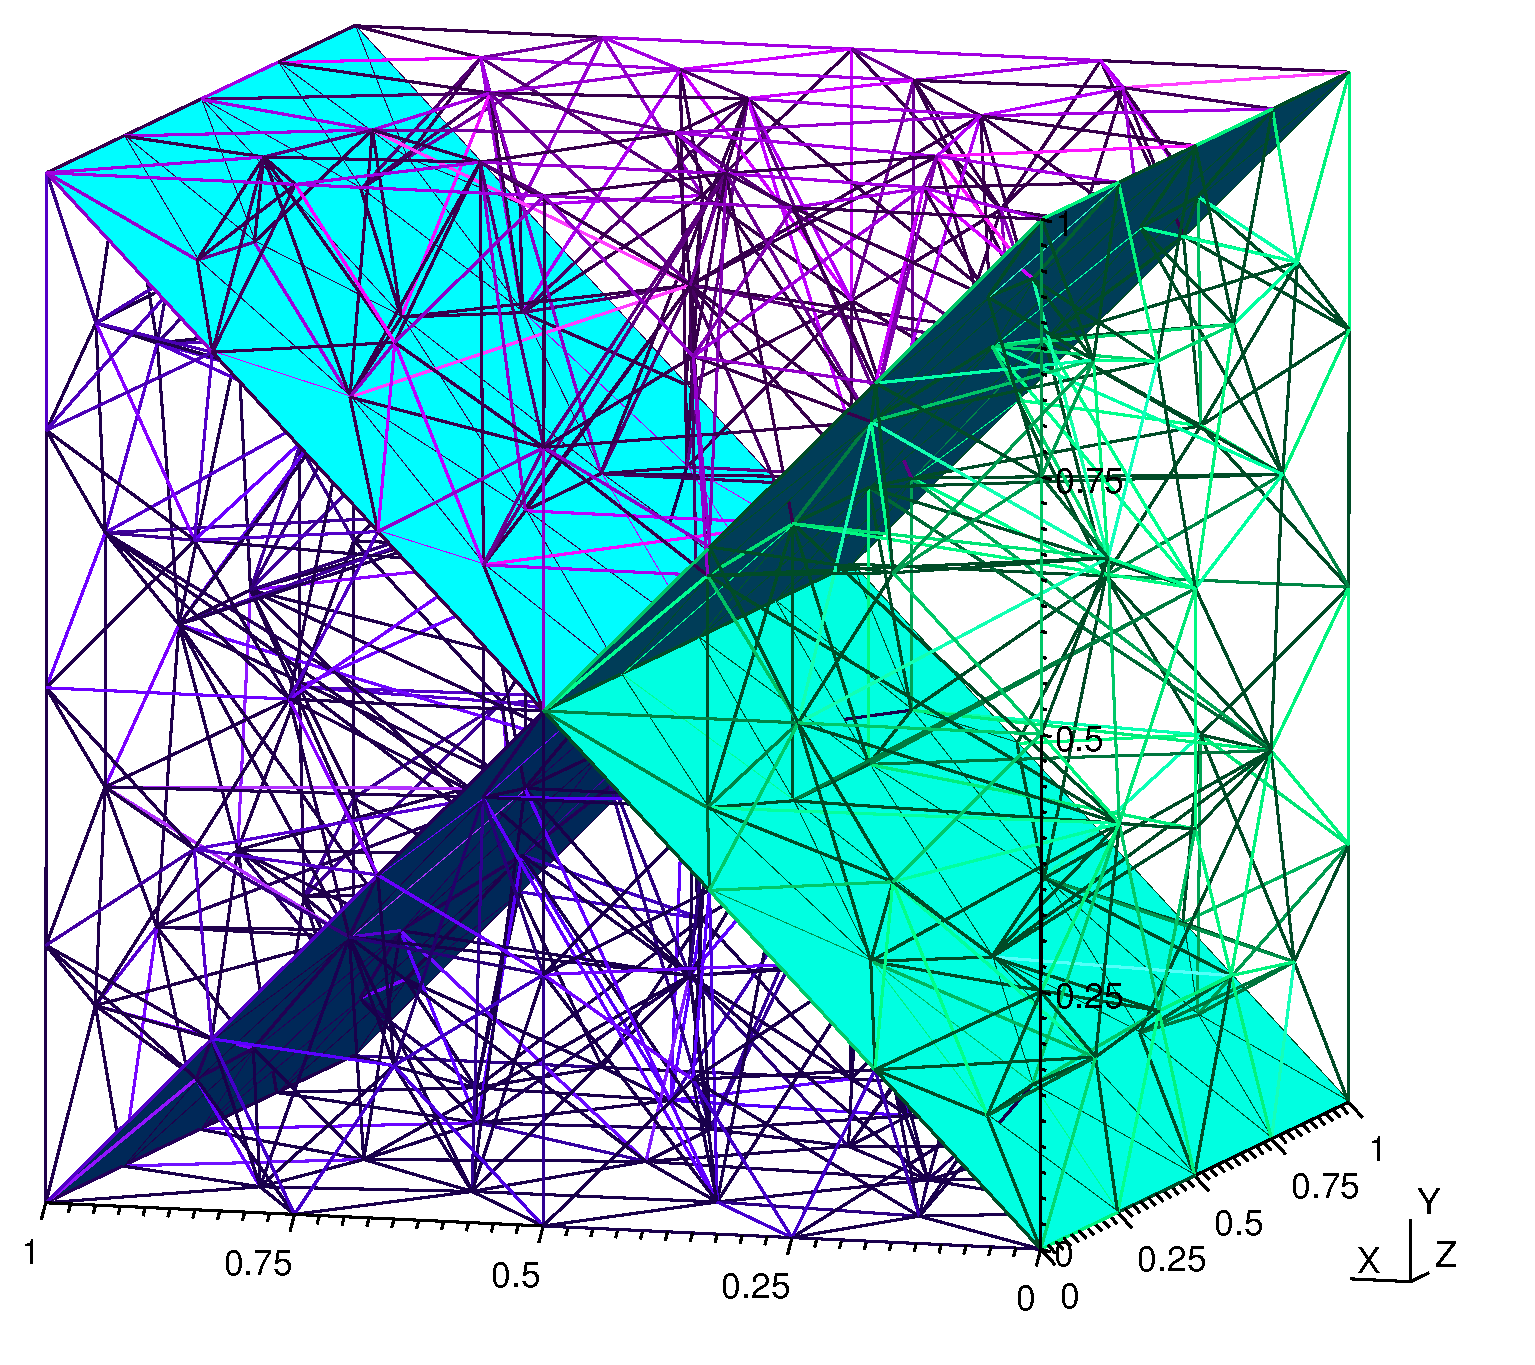
\includegraphics[width=13cm]{tests_graphics/01_mesh.pdf}
\caption{Test 01 -- mesh}
\label{fig:test1_mesh}
\end{figure}
%
%
\subsection*{Parameters}
\begin{itemize}
  \item \textbf{Cross section area:} 1D channel is set to 1.0~\unitss{}{2}{}.
  \item \textbf{Thickness:} 2D fractures are set to 1.0~\unitss{}{1}{}.
  \item \textbf{Conductivity:} The conductivity of materials:
    \begin{itemize}
      \item 1D channel is set to $K=10$~\unitss{}{1}{-1}.
      \item 2D fractures are set to $\mathbf{K}=\left(\begin{array}{cc} 1 & 0 \\ 0 & 1\end{array} \right)$~\unitss{}{1}{-1}.
      \item cube material is set to $\mathbf{K}=\left(\begin{array}{ccc} 0.1 & 0 & 0 \\ 0 & 0.1 & 0 \\ 0 & 0 & 0.1\end{array} \right)$~\unitss{}{1}{-1}.
    \end{itemize}
  \item There is no transport so there are not any other parameters.
\end{itemize}

\subsection*{Verification}
This test verifies solving steady Darcy flow by the mixed hybrid method. There are different dimensional connections 
which are 2D-3D connection between the cube and the flat fractures and 1D-2D connection between the 1D channel 
and the two flat fractures in their crossection. 

Following will not be commented in other examples and use of the functionalities will be considered apparent. No special test
programs are needed to test these as these are partially checked in the unit tests.

The input files \verb'flow_gmsh.con' and \verb'flow_vtk.con' give the same result, however the output is written in different 
formats. Also one can find an example of region set in \verb'flow_gmsh.con'.

Setting a Dirichlet boundary condition using piezometric head values is used in the input file \verb'flow_vtk_piezo.con'.
One can also notice using of the boundary set \verb'BOUNDARY' in this file. We use \emph{FieldFormula} to prescribe boundary
condition so this type of field and the function parser are also verified.

The remaining two files \verb'flow_old_vtk.con' and \verb'flow_vtk_fbc.con' use the obsolete way of defining boundary conditions.
The first one uses the old mesh without any named regions and the boundary condition file \verb'.fbc'. The second one combines
new mesh with named regions and the boudanry condition file created the old way. These tests ensure partially the backward 
compatibility of Flow123d with older input files.

%=====================================================
%                   TEST  2
%=====================================================

\section{Test 02 -- Steady flow in 2D and transport}
\label{sec:test02}
This test involves steady Darcy flow in 2D, connections of 1D-2D elements, Dirichlet boundary condition for flow and transport, 
transport of two substances with zero initial condition for concentration. There are actually two different cases computed in this test. 
Dual porosity and sorption features are present in the explicit transport. Dispersion is defined in the implicit transport.

The coefficient of diffusive transfer through a fracture (means between the fracture and the surrounding material) is set to 
zero so the substance cannot be diffused through the fracture's boundary.

  \begin{itemize} 
    \item \emph{problem type} -- sequential coupling 
    \item \emph{primary equation} -- steady mixed hybrid
    \item \emph{secondary equation} -- transport operator splitting (explicit), discontinuous Galerkin method (implicit)
  \end{itemize}

\subsection*{Geometry and boundary conditions}
The domain is two-dimensional slice through a part of a relief which involves several one-dimensional fractures.

Simple Dirichlet flow boundary condition is defined on left and right side where pressure heads are prescribed. 
There is no flow through the upper and lower boundary of the model. This all causes a flow along the x axis.

Dirichlet boundary condition for transport is prescribed on both sides as it is for flow boundary condition and 
the value of concentration is 1.0~\unitss{1}{-3}{} for both substances. Initial concentration of the substances 
is zero in the whole area. 
%
\begin{figure}[htb!]
\centering
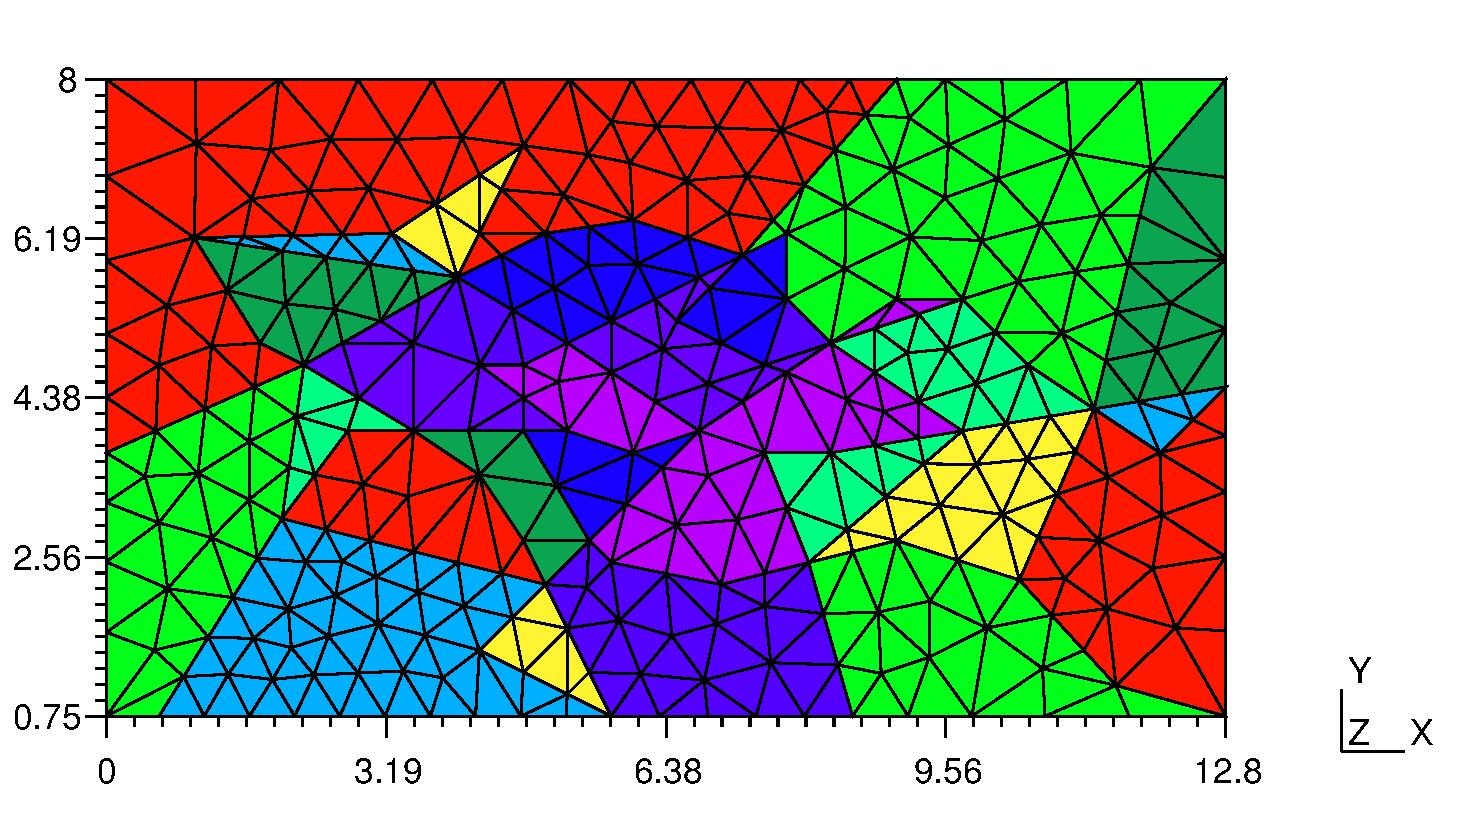
\includegraphics[width=15cm]{tests_graphics/02_mesh.pdf}
\caption{Test 02 -- mesh}
\label{fig:test2_mesh}
\end{figure}
%
%
\subsection*{Parameters}
The flow is steady and the transport is solved in time interval $(0,5.0)$~\unitss{}{}{1}. The output is written every 0.5~\unitss{}{}{1}. 
Time parameters for implicitly computed transport are the same only initial time step is set to 0.5~\unitss{}{}{1}.
\begin{itemize}
  \item \textbf{Cross section area:} 1D fractures are set to 1.0~\unitss{}{2}{}.
  \item \textbf{Thickness:} domain is set to 1.0~\unitss{}{1}{}.
  \item \textbf{Conductivity:} The conductivity of materials:
    \begin{itemize}
      \item fracture material is set to $K=10$~\unitss{}{1}{-1}.
      \item plane material is set to $\mathbf{K}=\left(\begin{array}{cc} 1 & 0 \\ 0 & 1\end{array} \right)$~\unitss{}{1}{-1}.
    \end{itemize}
  \item \textbf{Sorption:} The sorption parameters are for both materials equal:
    \begin{itemize}
      \item linear sorption isotherm parameter of the first substance is set to $k_l=0.02$.
      \item Freundlich sorption isotherm parameters of the second substance are set to $k_F=0.02$, $\alpha=0.5$  
    \end{itemize}
  \item \textbf{Dual porosity:} The dual porosity parameters are for both materials equal:
    \begin{itemize}
      \item mobile porosity coefficient is set to $0.25$
      \item immobile porosity coefficient is set to $0.25$
      \item nonequilibrium coefficient of both substances $0.01$
    \end{itemize}
  \item \textbf{Dispersion coefficients:} No dispersion is involved.
\end{itemize}

\subsection*{Verification}
This test verifies explicitly computed transport considering only convection with dual porosity and sorption and implicitly 
computed transport considering both convection and dispersion. Transport through 1D-2D element connections is computed in addition to the first test.



%=====================================================
%                   TEST  03
%=====================================================

\section{Test 03 -- Steady flow in 2D and transport}
\label{sec:test03}
This test differs from the previous one only by simpler structure of its geometry. It shows how the substace flows in the main fracture and divides in two other fractures. The substance spreads in the fractures much faster in comparision to transport in the plane.
\subsection*{Geometry and boundary conditions}
There is a plane with side 1.0 which is cutted by fractures. The main fracture divides in two other fractures.
\subsection*{Parameters}
The flow is steady and the transport is solved in time interval $(0,1.0)$. The output is written every 0.01. Initial time step for transport computed implicitly is set to 0.1 and the output is written every 0.1.

Other parameters are the same as in test 02.
\subsection*{Verification}
This test verifies the same features as the test 02 does but on a simpler geometry.



%=====================================================
%                   TEST  05
%=====================================================

\section{Test 05 -- Darcy flow boundary conditions}
\label{sec:test05}
There are three types of boundary conditions -- Dirichlet, Neumann and Robin that are tested. All three test have the same geometry and boundary conditions are derived from the same analytical solution.

We will prescribe analytical solution $u=xy$ of Laplace equation $-\Lapl{}u = 0$.
\begin{itemize} 
    \item \emph{problem type} -- sequential coupling 
    \item \emph{primary equation} -- steady mixed hybrid
  \end{itemize}

\subsection*{Geometry and boundary conditions}
The geometry is simple -- square plane in xy coordinates with corner points [0,0] and [1,1]. Each side has its own boundary regions called \verb0.bc_south0, \verb0.bc_east0, \verb0.bc_north0, \verb0.bc_west0.

\textbf{Dirichlet test.} All sides have pressure prescribed. These are south: $u_D=0$; east: $u_D=y$; north: $u_D=x$; west: $u_D=0$.

\textbf{Neumann test.} Two sides have pressure prescribed for the Dirichlet boundary condition: east: $u_D=y$; west: $u_D=0$. Two other sides have flux prescribed: south: $q_N=x$; north $q_N=-x$.

\textbf{Robin test.} Two sides have pressure prescribed  for the Dirichlet boundary condition: east: $u_D=y$; west: $u_D=0$.
For Robin boundary condition we get from the equation boundary pressure
\begin{equation} 
u_R=\frac{1+\sigma_R}{\sigma_R}x. 
\end{equation}
We choose $\sigma_R=0.5$ and then we get $u_R=-2x$ on the south side and $u_R=3x$ on the north side. 

\subsection*{Parameters}
\begin{itemize}
  \item \textbf{Conductivity:} on region \verb0plane0 is $1.0$~\unitss{}{1}{-1}.
  \item \textbf{Thickness:} on region \verb0plane0 is by default 1.0~\unitss{}{1}{}.
  \item There are no other regions, no transport so there are not any other parameters.
\end{itemize}

\subsection*{Verification}
This test verifies prescribing different types boundary conditions.


%=====================================================
%                   TEST  06
%=====================================================

\section{Test 06 -- Coupling between dimensions in Darcy flow}
\label{sec:test06}
There are two tests -- \verb'flow_32d.con' for compatible coupling between 3D-2D and \verb'flow_21d.con' for compatible coupling between 2D-1D.

\begin{itemize} 
    \item \emph{problem type} -- sequential coupling 
    \item \emph{primary equation} -- steady mixed hybrid
  \end{itemize}

We will discuss both the geometry and parameters at once.

%
\begin{figure}[h!]
\centering
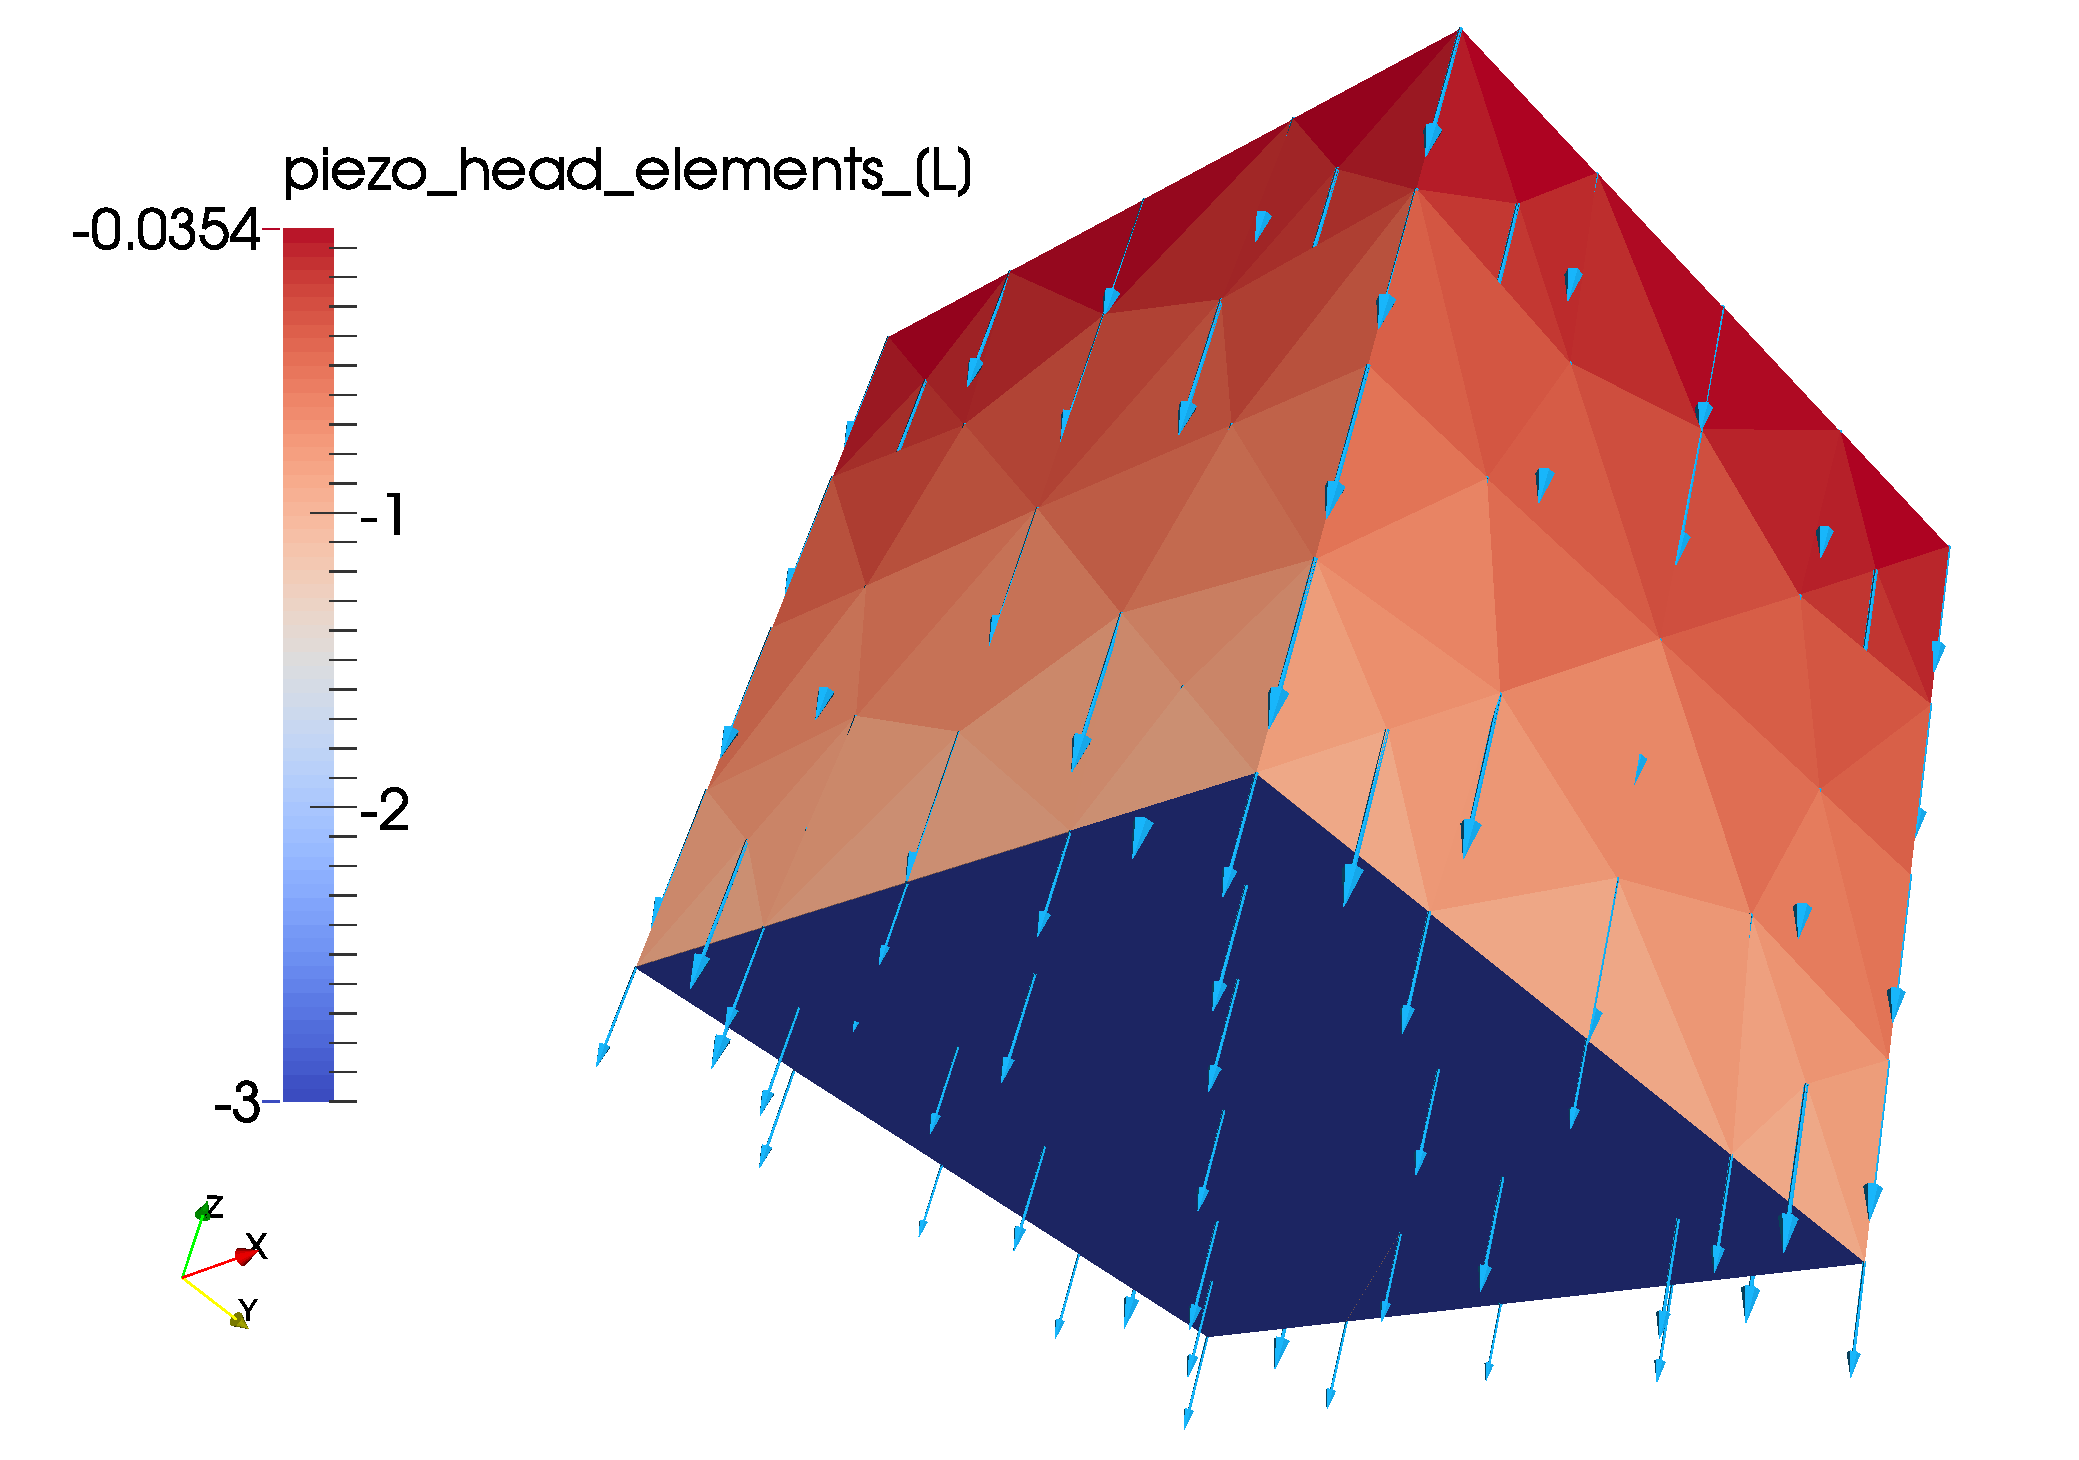
\includegraphics[width=0.6\textwidth]{tests_graphics/06_result_32d.pdf}
\caption{Test 06 -- solution. For verification see the blue plate where the constant piezometric head is.}
\label{fig:test6_solution_32d}
\end{figure}
%
\textbf{3D-2D.}
There is a cube with vertices [0,0,0] [-1,-1,-1] which couples with a 2D crack in the bottom (i.e. $z=-1$~\unitss{}{1}{}).
We consider solution of the piezometric head in the cube $p_3(x,y,z) = z$. We will use it to prescribe Dirichlet boundary condition on the non-coupling parts of the cube.
There are no sources of a flow in the cube. 
We can write the outflow through the bottom of the cube in following term $q_{32} = \mathbf{q_3} \cdot \mathbf{n} = (- K_3 \nabla p_3(x,y,-1))\cdot \mathbf{n}$,
where $\mathbf{n}=(0,0,-1)$.
To obtain Laplace equation with zero right hand side on the 2D crack, we prescribe a new source term (\ref{eqn:test06_f2}) that eliminates the inflow coming from the cube.         
\begin{eqnarray}
    F_2 &=& \delta_2  f_2 + q_{32} = 0   \nonumber\\
    f_2(x,y) &=& -\frac{q_{32}}{\delta_2}   \label{eqn:test06_f2}.
\end{eqnarray}
When $\delta_2 = 10$~\unitss{}{1}{}, $K_3 = 2$~\unitss{}{1}{-1} are choosed then the source term is equal $f_2 = -0.2$~\unitss{}{}{-1}.
Homogenous Neumann condition is prescribed on the boundary of the fraction (zero outflow and inflow).

From the flow coupling equation we can get the piezometric head (\ref{eqn:test06_p2}) on the crack which we can verify.
\begin{eqnarray} 
     \sigma_{32}  ( p_3(x,y,-1) - p_2(x,y) ) &=& q_{32} \nonumber\\
     p_2(x,y) &=& -\frac{q_{32}}{\sigma_{32}} + p_3(x,y,-1) \label{eqn:test06_p2}.
\end{eqnarray}   
When $\sigma_{32} = 1$~\unitss{}{}{-1} is set then the piezometric head in the crack is constant and equal $p_2(x,y) = -3$~\unitss{}{1}{}.

%
\begin{figure}[h!]
\centering
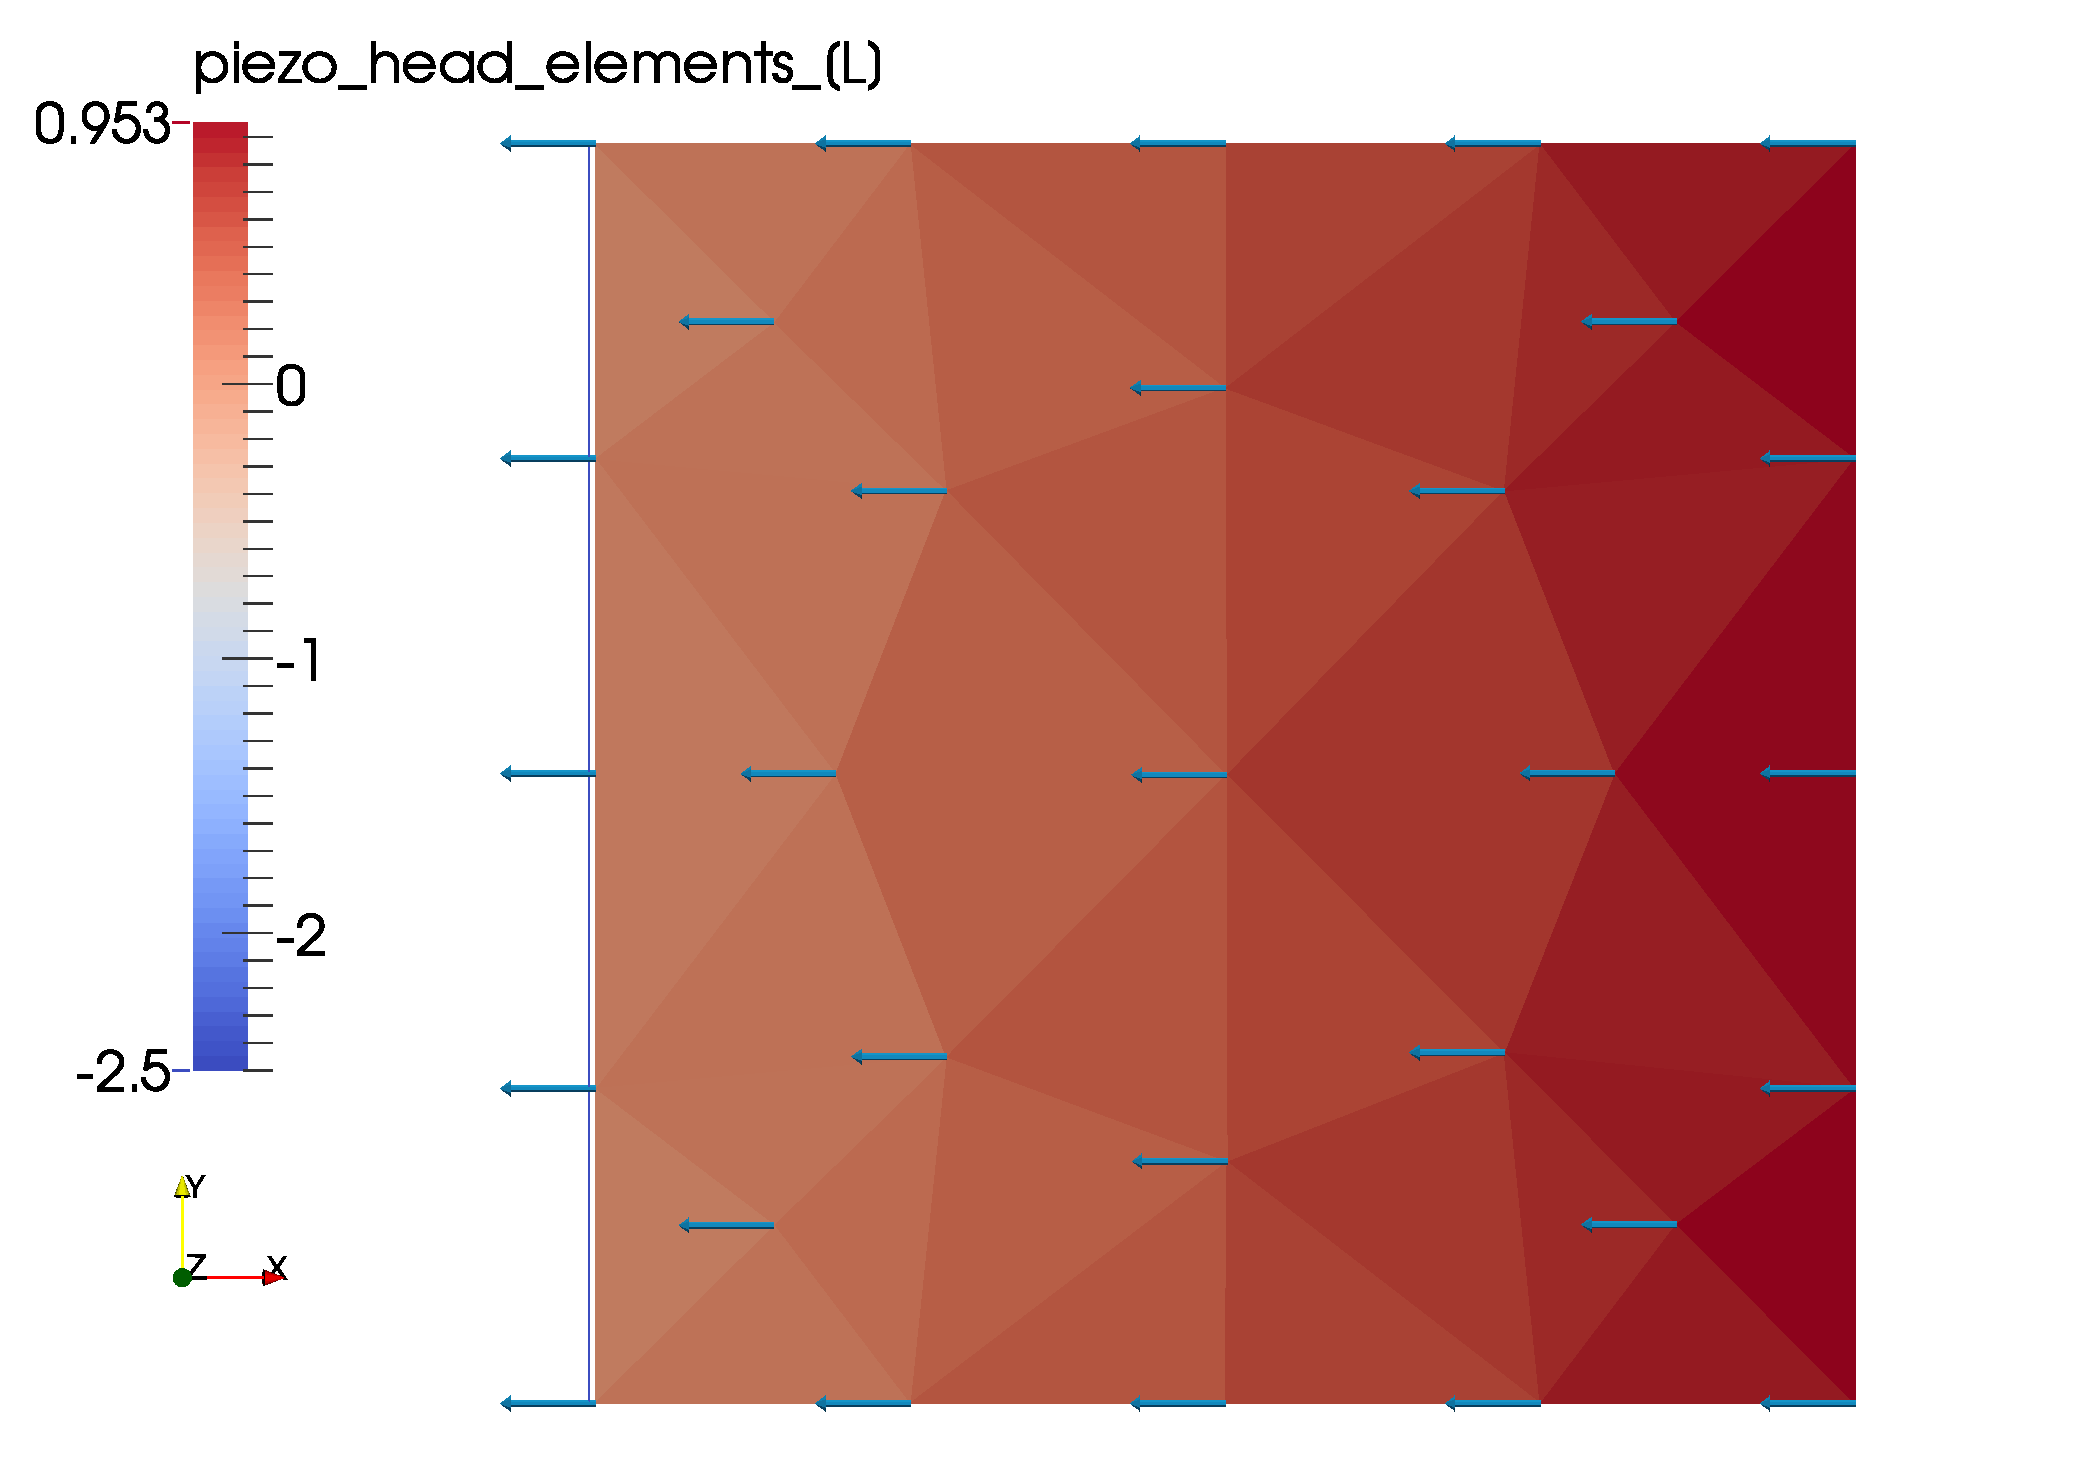
\includegraphics[width=0.6\textwidth]{tests_graphics/06_result_21d.pdf}
\caption{Test 06 -- solution. For verification see the blue channel on the left side of the plane where the constant piezometric head is.}
\label{fig:test6_solution_32d}
\end{figure}
%
\textbf{2D-1D.}
The other tests geometry consists of a 2D crack in $xy$ plane with vertices [0,0] [1,1] and a 1D channel coupling with the crack on the left side ($x=0$). 
Everything is then analogical to the first test.
We consider solution of the pressure in the crack $p_2(x,y) = x$. We will use it to prescribe Dirichlet boundary condition on the non-coupling parts of the crack.
There are no sources of a flow in the crack. 
We can write the outflow through the left side of the crack in the following term $q_{21} = \mathbf{q_2} \cdot \mathbf{n} = (- \delta_2 K_2 \nabla p_2(0,y))\cdot \mathbf{n}$,
where $\mathbf{n}=(-1,0)$.
To obtain Laplace equation with zero right hand side on the channel, we prescribe a new source term (\ref{eqn:test06_f1}) that eliminates the inflow coming from the crack.         
\begin{eqnarray}
    F_1 &=& \delta_1  f_1 + q_{21} = 0   \nonumber\\
    f_1(x,y) &=& -\frac{q_{21}}{\delta_1}   \label{eqn:test06_f1}.
\end{eqnarray}
When $\delta_1 = 20$~\unitss{}{2}{}, $\delta_2 = 10$~\unitss{}{1}{} and $K_2 = 5$~\unitss{}{1}{-1} are choosed then the source term is equal $f_2 = -2.5$~\unitss{}{}{-1}.
Homogenous Neumann condition is prescribed on the boundary of the fraction (zero outflow and inflow).

From the flow coupling equation we can get the pressure (\ref{eqn:test06_p1}) on the plane which we can verify.
\begin{eqnarray} 
     \delta_2 \sigma_{21} ( p_2(0,y) - p_2(y) ) &=& q_{21} \nonumber\\
     p_1(y) &=& -\frac{q_{21}}{\delta_2 \sigma_{21}} + p_2(0,y) \label{eqn:test06_p1}.
\end{eqnarray}   
When $\sigma_{21} = 1$~\unitss{}{}{-1} is set then the pressure in the crack is constant and equal $p_1(y) = -2.5$~\unitss{}{1}{}.

% \subsection*{Parameters}
% Parameters where discussed above.

\subsection*{Verification}
This test verifies correct communication between dimensions 3D-2D and 2D-1D in compatible coupling.
We can also observe the results in the \verb'water_balance' file. We should see that all the inflow 
to the cube should be fully compensated by the negative source. Homogenous Neumann boundary condition 
is prescribed on the crack so there should be no outflow or inflow through the boundary of the crack.
The situation in the second test is similar. The inflow to the crack should be fully compensated by 
the negative source in the channel which should have no other inflow or outflow.


%=====================================================
%                   TEST  8
%=====================================================

\section{Test 08 -- Steady Darcy flow with source}
\label{sec:test08}
This test is aimed at verifying steady Darcy flow with source which is prescribed by function formula. 
We will solve Laplace equation $-\Lapl{}u = f$ where source $f$ is prescribed by function $f = 2(1-y^2) + 2(1-x^2)$.
We can easily prove that (\ref{eqn:test8}) is the analytic solution by replacing it in the Laplace equation.
\begin{equation}
u = (1-x^2)(1-y^2) \label{eqn:test8}
\end{equation}

  \begin{itemize} 
    \item \emph{problem type} -- sequential coupling 
    \item \emph{primary equation} -- steady mixed hybrid
  \end{itemize}

\subsection*{Geometry and boundary conditions}
The domain is a square with opposite vertices $[-1,-1]$ and $[1,1]$. Zero dirichlet boundary condition is prescribed 
on all boundaries -- along the circumference of the square.
 
\subsection*{Parameters}
\begin{itemize}
  \item \textbf{Conductivity:} The conductivity of plane material is $1.0$~\unitss{}{1}{-1}.
  \item There are no other materials, no transport so there are not any other parameters.
\end{itemize}
%
\begin{figure}[h!]
\centering
\includegraphics[width=0.8\textwidth]{tests_graphics/08_result.pdf}
\caption{Test 08 -- solution. Distribution of the pressure matches the analytical solution (\ref{eqn:test8}).}
\label{fig:test8_solution}
\end{figure}
%
\subsection*{Verification}
The solution (pressure) is a paraboloid with a top in $[0,0,1]$ as we can see in the figure \ref{fig:test8_solution}. 
One can verify the equality in Paraview using the prepared state file.


%=====================================================
%                   TEST  10
%=====================================================

\section{Test 10 -- Unsteady flow in 2D}
\label{sec:test10}
Unsteady flow in 2D domain is simulated in this test and is computed by both mixed hybrid and 
lumped mixed hybrid method. No transport is involved. 

\begin{itemize} 
    \item \emph{problem type} -- sequential coupling
    \item \emph{primary equation} -- unsteady mixed hybrid, unsteady lumped mixed hybrid
  \end{itemize}

\subsection*{Geometry and boundary conditions}
The domain is a square with oposite vertices $[0,0]$ and $[1,1]$. Different Dirichlet boundary condition for 
pressure is prescribed on two opposite sides -- 0.0~\unitss{}{1}{} on the left and 100.0~\unitss{}{1}{} on the right.

\subsection*{Parameters}
The flow is solved in time interval $(0,0.5)$ with step 0.01~\unitss{}{}{1}. The output is written every 0.1~\unitss{}{}{1}.
\begin{itemize}
  \item \textbf{Conductivity:} The conductivity of plane material is $0.02$~\unitss{}{1}{-1}.
  \item Initial pressure is set to zero everywhere.
  \item There are no other materials, no transport so there are not any other parameters.
\end{itemize}

\subsection*{Verification}
This test verifies two different numerical methods -- the problem is computed by both mixed hybrid and lumped mixed hybrid method.

%=====================================================
%                   TEST  11
%=====================================================

\section{Test 11 -- Radioactive decay chain with more branches}
8 isotopes are members of considered decay chain with three branches. Transport boundary conditions does not matter 
because zero presure gradient is considered. Final concentrations of all isotopes except C decrease to zero after 20 
time steps, whereas C concentration grows to 0.36.
\[
 E\xrightarrow{}D\xrightarrow{}F\xrightarrow{}B
 \quad
 \begin{matrix}
    0.2B\xrightarrow{}A & A\xrightarrow{}G \\
    0.6B\xrightarrow{}H & H\xrightarrow{}G \\
    0.2B\xrightarrow{}G &\\
 \end{matrix}
 \quad
 G\xrightarrow{}C 
\]

\begin{itemize} 
    \item \emph{problem type} -- sequential coupling
    \item \emph{primary equation} -- steady mixed hybrid
    \item \emph{secondary equation} -- transport operator splitting
    \item \emph{reactions} -- linear reactions
  \end{itemize}

\subsection*{Geometry}
The domain is a prism which base is a right-angled triangle with its ordinates 3.0~\unitss{}{1}{}. 
There are only three tetrahedron elements in the mesh.

\subsection*{Parameters}
The flow is steady and the transport is solved in time interval $(0,10.0)$~\unitss{}{}{1}. The output is written every 0.5~\unitss{}{}{1}.

Half-lives are equal to 0.5 for all isotopes. Initial concentrations are summarized in the table below:
  \begin{center}
    \begin{tabular}[c]{|l|c|c|c|c|c|c|c|c|}
      \hline
      isotop & A & B  & C & D & E & F & G & H \\[4pt]
      initial concentration & 0.01 & 0.02 & 0.03 & 0.04 & 0.05 & 0.06 & 0.07 & 0.08 \\[4pt]
      \hline
    \end{tabular}
  \end{center}


\subsection*{Verification}


%=====================================================
%                   TEST  12
%=====================================================

\section{Test 12 -- Radioactive decay}
There are actually two tests of the radioactive decay. The first one considers first order reaction of two isotopes 
determined by kinetic constant and the other one describes radioactive decay chain of three isotopes.

\begin{itemize} 
    \item \emph{problem type} -- sequential coupling
    \item \emph{primary equation} -- steady mixed hybrid
    \item \emph{secondary equation} -- transport operator splitting
    \item \emph{reactions} -- linear reactions
  \end{itemize}

\subsection*{Geometry and boundary conditions}
The domain is a prism which base is a right-angled triangle with its ordinates 3.0 units long. There are then only three tetrahedron elements in the mesh.

There are two Dirichlet boundary conditions for flow prescribed.

\begin{itemize}
  \item \textbf{Conductivity:} The conductivity of the prism material is $0.01$~\unitss{}{1}{-1}. 
  \item There is no other parameter for flow or transport.
\end{itemize}



\subsection{First order reaction determined by kinetic constant}
The only linear reaction between D and F substances.
\[
D\xrightarrow{k}F
\]

\subsection*{Parameters}
The flow is steady and the transport is solved in time interval $(0,10.0)$. The output is written every 0.5~\unitss{}{}{1}.  
\begin{itemize}
  \item \textbf{Substances:} 6 substances to be transported -- A, B, C, D, E, F
  \item \textbf{Kinetic constant:} $k = 0.277258872$
\end{itemize}

\subsection*{Verification}

\subsection{Radioactive decay chain}
The considered radioctive decay chain is:
\[
 D\xrightarrow{t_{1/2,D}}F\xrightarrow{t_{1/2,F}}B
\]
\subsection*{Parameters}
Time parameters are the same as they are above.
\begin{itemize}
  \item \textbf{Substances:} 6 substances to be transported -- A, B, C, D, E, F
  \item \textbf{Decay half-lives:} $t_{1/2,D} = t_{1/2,F} = 2.5$
\end{itemize}

\subsection*{Verification}

% Both following tests are realized without combination with transport (zero pressure gradient).
% verification of:
% - first order reaction A->B determined by kinetic constant,
% -- 6 chemical species (A, B, .., F) are transported but just 2 of them take a part in considered first order kinetic reaction wich looks as follows
% --- D->F, appropriate kinetic constant is k = 0.277258872.
% --- Initail conditions look as follows, A(0) = 0.01, B(0) = 0.02, C(0) = 0.03, D(0) = 0.04, E(0) = 0.05, F(0) = 0.06.
% --- Transport boundary conditions does not matter because zero presure gradient is considered.
% --- Final concentrations of all isotopes except A, B, C, E do not change. Concentrations of D decreases to 0.003. Concentration of F increase to 0.85 in 20 time steps.

% - narrow radioctive decay chain without branches, A -> B -> C,
% -- 6 isotopes (A, B, .., F) are transported but just 3 of them are members of considered decay chain which looks as folows
% --- D->F->B
% --- Initail conditions look as follows, A(0) = 0.01, B(0) = 0.02, C(0) = 0.03, D(0) = 0.04, E(0) = 0.05, F(0) = 0.06.
% --- Transport boundary conditions does not matter because zero presure gradient is considered.
% --- Final concentrations of all isotopes except A, C, E do not change. Concentrations of D and B decrease to 0.004 and 0.012 respectively. Concentration of B increase to 0.1 in 20 time steps.

%=====================================================
%                   TEST  13
%=====================================================

\section{Test 13 -- Solute mixing on the edge}
This test realizes mixing of substances on the edges of planes and also does quantitative test on a trivial 
transport problem. The problem is computed with both explicit and implicit transport.

\begin{itemize} 
    \item \emph{problem type} -- sequential coupling 
    \item \emph{primary equation} -- steady mixed hybrid
    \item \emph{secondary equation} -- transport operator splitting (explicit), discontinuous Galerkin method (implicit)
  \end{itemize}

\subsection*{Geometry and boundary conditions}
The domain is a fork where the main branch with the incoming solute is 5~\unitss{}{1}{} long and lies in 
the $xy$ plane. Then it is divided into two other branches $5\sqrt{2}$~\unitss{}{1}{} long, one with 
positive and the another with negative $z$ coordinate. There are different conductivities in each branch.

Dirichlet boundary conditions for flow and transport are prescribed at the beginning of the main 
plane ($x=0$~\unitss{}{1}{}) and at the ends of the secondary branches ($x=10$~\unitss{}{1}{}).

flow: $h_D=-x-z+10.0$ which gives 10.0~\unitss{}{1}{} at point [0,0,0] and $\pm5$~\unitss{}{1}{} at points [10,0,$\mp5$]\\
transport: concentration is 1.0 at point [0,0,0] and 0.0 at points [10,0,$\mp5$]

Initial concentration of the substances is zero in the whole area. 
%
\begin{figure}[htb!]
\centering
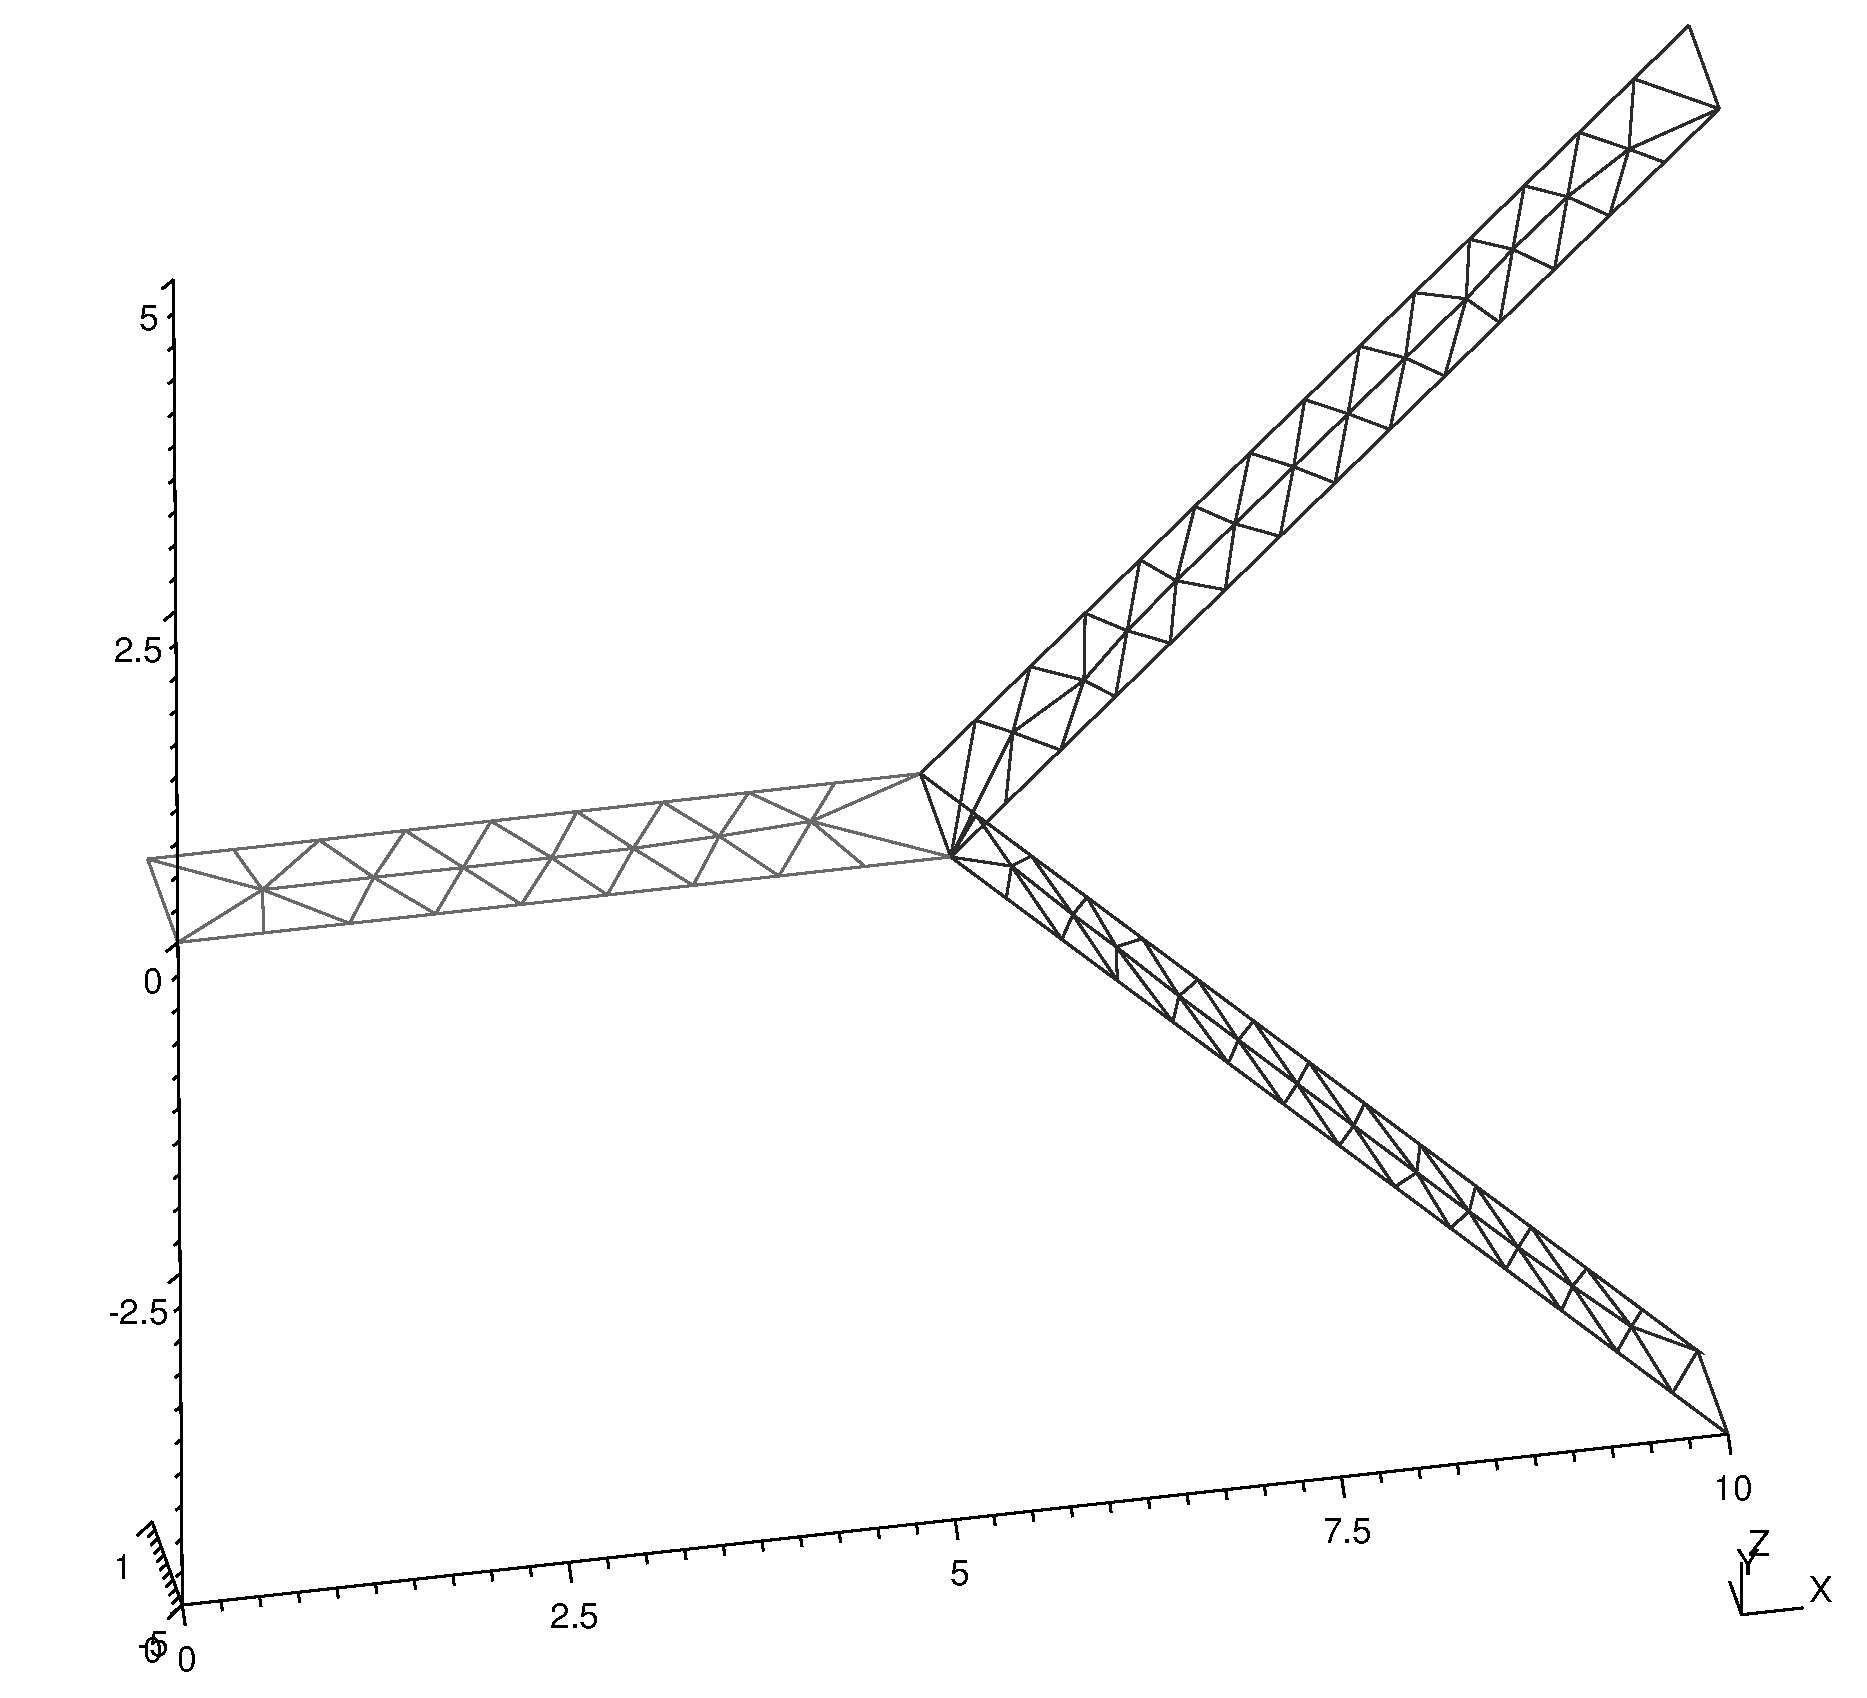
\includegraphics[width=12cm]{tests_graphics/13_mesh.pdf}
\caption{Test 13 -- mesh}
\label{fig:test13_mesh}
\end{figure}
%
%
\subsection*{Parameters}
The flow is steady and the transport is solved in time interval $(0,100.0)$~\unitss{}{}{1}. 
The output is written every 0.5~\unitss{}{}{1}. 
Time parameters for implicitly computed transport are the same only initial time step and output time is set to 5.0~\unitss{}{}{1}.
\begin{itemize}
  \item \textbf{Thickness:} all planes are set to 1.0~\unitss{}{1}{}.
  \item \textbf{Conductivity:} The conductivity of materials (isotropic planes):
    \begin{itemize}
      \item main branch (material num. 17): $K=1$~\unitss{}{1}{-1}.
      \item branch (positive $z$, material num. 18): $K=0.1$~\unitss{}{1}{-1}.
      \item branch (negative $z$, material num. 19): $K=0.1$~\unitss{}{1}{-1}.
    \end{itemize}
  \item \textbf{Dispersion coefficients:} Default parameters are set in implicit transport, so no dispersion is present. 
        For more details see \hyperlink{IT::TransportDG-BulkData}{TransportDG\_BulkData} in the input reference.
\end{itemize}

\subsection*{Verification}
This test verifies qualitatively both the problem of flow and transport.

%=====================================================
%                   TEST  14
%=====================================================

\section{Test 14 -- Variable transport boundary condition}
We consider a time variable boundary condition for transport in this test. Steady flow with constant velocity is caused by a pressure 
gradient from one side of a 2D strip to the another. Dirichlet boundary condition for transport evolving in time is prescribed on the 
right side using set of older \verb'.tbc' files. 

\begin{itemize} 
    \item \emph{problem type} -- sequential coupling, 
    \item \emph{primary equation} -- steady mixed hybrid
    \item \emph{secondary equation} -- transport operator splitting (explicit), discontinuous Galerkin method (implicit)
  \end{itemize}

\subsection*{Geometry and boundary conditions}

Dirichlet boundary condition for pressure is prescribed $x$ all around the plane and causes constant flow from right to left 
(pressure prescribed on the upper and lower sides are equal along x axis so causes no flow). Transport boundary condition has 
the same prescribtion as for the pressure, only the values evolves in time.

Initial concentration is zero on the whole plane. Two pulses of nonzero concentration are applied on the boundary. The changes 
of the boundary condition at specified times are shown in the following table:
%
\begin{center}
  \begin{tabular}{|l|c|c|c|c|c|}
    \hline
    time \units{}{1}{} & $0$ & $1$ & $3$ & $6$ & $7$\\
    concentration & $0$ & $20$ & $0$ & $40$ & $0$\\
    \hline
  \end{tabular}
\end{center}

\begin{figure}[htb!]
\centering
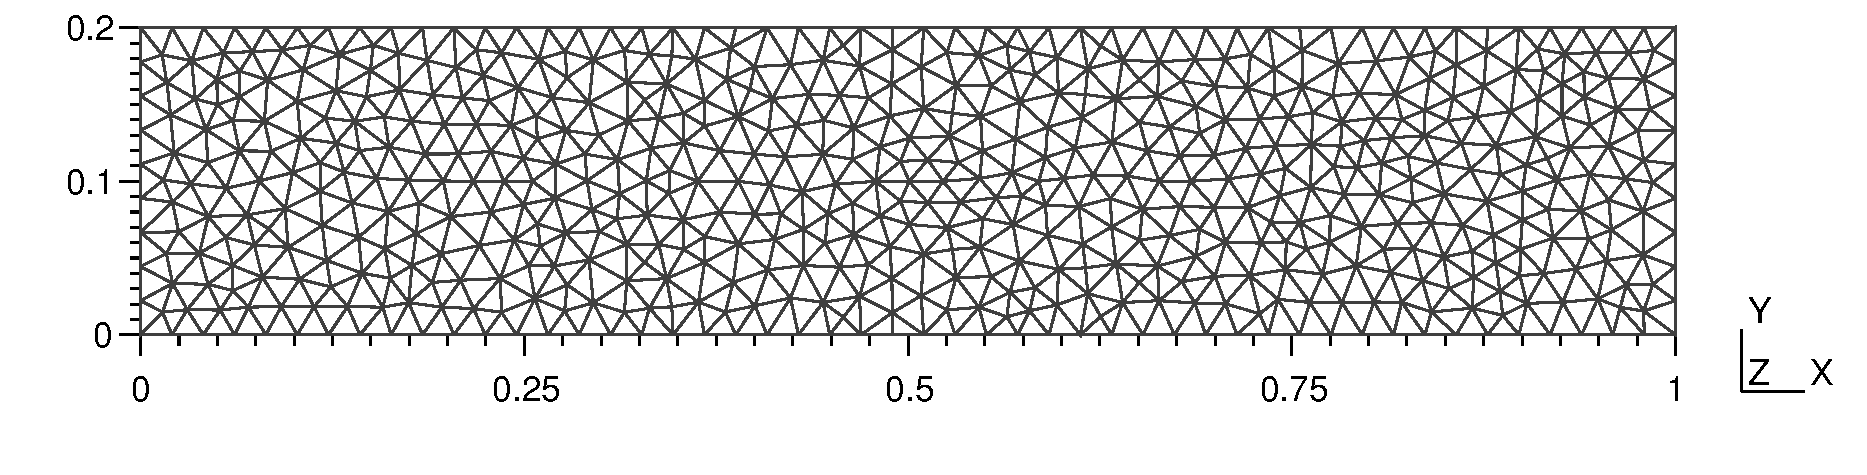
\includegraphics[width=15cm]{tests_graphics/14_mesh.pdf}
\caption{Test 14 -- mesh}
\label{fig:test14_mesh}
\end{figure}
%
%
\subsection*{Parameters}
The flow is steady and the transport is solved in time interval $(0,10.0)$~\unitss{}{}{1}. The output is written every 
1.0~\unitss{}{}{1}. Time parameters for implicitly computed transport are the same only initial time step is set to 1.0~\unitss{}{}{1}.
%
\begin{itemize}
  \item \textbf{Thickness:} all planes are set to 1.0~\unitss{}{1}{}.
  \item \textbf{Conductivity:} The conductivity of material (isotropic plane): $K=0.1$~\unitss{}{1}{-1}.
  \item \textbf{Dispersion coefficients:} Default parameters are set in implicit transport, so no dispersion is present. 
        For more details see \hyperlink{IT::TransportDG-BulkData}{TransportDG\_BulkData} in the input reference.
\end{itemize}
%

\subsection*{Verification}



%=====================================================
%                   TEST  15
%=====================================================

\section{Test 15 -- Unsteady flow with transport}
Transport of a single pulse of concentration moving along a 2D strip is solved. This test involves unsteady flow computed by lumped hybrid method, transport is solved both with explicit and implicit (involves dispersion) scheme.
 
\begin{itemize} 
    \item \emph{problem type} -- sequential coupling, 
    \item \emph{primary equation} -- unsteady lumped mixed hybrid
    \item \emph{secondary equation} -- transport operator splitting (explicit), discontinuous Galerkin method (implicit)
  \end{itemize}

\subsection*{Geometry and boundary conditions}
The domain is a 2D strip with dimensions $1.0$x$16.0$. Zero Dirichlet boundary for flow is prescribed at $x=0$, zero Neumann boundary is elsewhere. 

Dirichlet transport boundary condition is set on the left side to 10.0 only at the beginning. Then is this boundary condition zero.

\subsection*{Parameters}
Initial pressure is zero everywhere. 
The source is prescribed with function $f=-x$ along the strip.
%
\begin{itemize}
  \item \textbf{Thickness:} all planes are set to 1.0~$L$.
  \item \textbf{Conductivity:} The conductivity of material (isotropic plane): $K=1.0$.
  \item \textbf{Source formula:} $f = -x$
  \item \textbf{Diffusivity coefficients:} are used in implicit transport wth dispersion. 
	Default parameters are set ($d_m=1e-6$, others are zero, see manual or parameters in test02 in ~\ref{sec:test02}).
\end{itemize}
%
\begin{figure}[htb!]
\centering
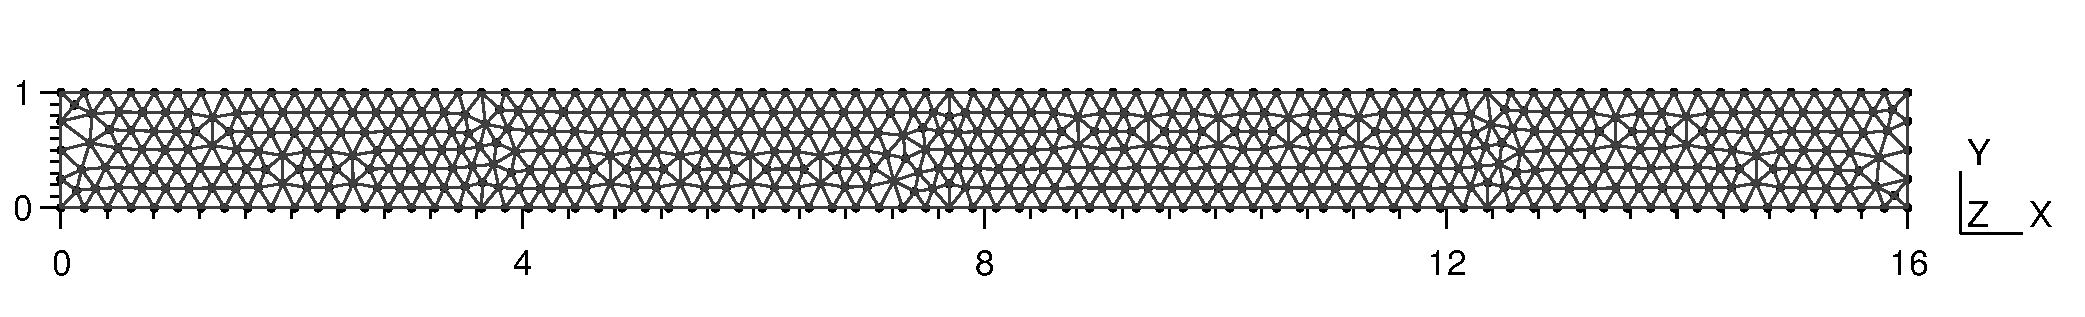
\includegraphics[width=15cm]{tests_graphics/15_mesh.pdf}
\caption{Test 15 -- mesh}
\label{fig:test15_mesh}
\end{figure}
%
%
\subsection*{Verification}
The test is similar to the test 10 but here in addition the computation of a transport in an unsteady flow field is verified.


%=====================================================
%                   TEST  16
%=====================================================

\section{Test 16 -- Substance concentration source in transport}
This test include a source of concentration of a substance. The domain is a 2D strip in vertical direction. There is a steady flow with constant velocity in the vertical direction. Two sources are situated on two elements at the top of the strip and the substance is transported down along the strip. The concentration values of the sources are defined in the \verb0tso0 input file.

\begin{itemize} 
    \item \emph{problem type} -- sequential coupling, 
    \item \emph{primary equation} -- steady mixed hybrid
    \item \emph{secondary equation} -- transport operator splitting
  \end{itemize}

\subsection*{Geometry}


\subsection*{Parameters}

\subsection*{Verification}



%=====================================================
%                   TEST  17
%=====================================================

\section{Test 17 -- Radioactive decay -- Pade approximation}
This test solves radioactive decay chain of five isotopes using Pade approximation.
The considered radioctive decay chain is:
\[
 A\xrightarrow{t_{1/2,A}}B\xrightarrow{t_{1/2,B}}C\xrightarrow{t_{1/2,C}}D\xrightarrow{t_{1/2,D}}E
\]

\begin{itemize} 
    \item \emph{problem type} -- sequential coupling, 
    \item \emph{primary equation} -- steady mixed hybrid
    \item \emph{secondary equation} -- transport operator splitting
    \item \emph{reactions} -- Pade approximation
  \end{itemize}

\subsection*{Geometry}
The geometry and material and transport parameters are the same as in test 12.


\subsection*{Parameters}
\begin{itemize}
  \item \textbf{Substances:} 5 substances to be transported -- A, B, C, D, E
  \item Polynomial degree of the nominator and the denominator of Pade approximation is~3.
  \item \textbf{Decay half-lives:} 
    \begin{tabular}[c]{|c|c|c|c|}
      \hline
      $t_{1/2,A}$ & $t_{1/2,B}$  & $t_{1/2,C}$ & $t_{1/2,D}$\\[4pt]
      $1.3863$ & $2.3105$ & $1.5403$ & $1.1552$\\[4pt]
      \hline
    \end{tabular}
\end{itemize}

\subsection*{Verification}


%=====================================================
%                   TEST  18
%=====================================================

\section{Test 18 -- Diffusion through fractures}
This test is aimed at transport caused just by diffusion. 

There is a triangular domain with zero pressure everywhere so no flow is present. Triangular element with high concentration of a substance lies in the middle of the domain and its sides neighbour with fractures.
The coeffients of molecular diffusion and diffusive transfer through fractures are the parameters of the implicit transport and are set in the configuration file.

\subsection*{Geometry}

\subsection*{Parameters}

\subsection*{Verification}






% ===================  PREPARING  ==================
% \section{Test 20 -- Dirichlet boundary condition}
% \label{sec:test20}
% This test involves steady Darcy flow in 3D determined by Dirichlet boundary condition. The analytic solution is prescribed $u = xyz$. We can see from the formula that there are no sources $-\Lapl{}u = 0$ (zero right hand side) and we can easily define Dirichlet boundary conditions on the sides of the cube just by evaluating the solution there.
% 
% \subsection*{Geometry}
% The domain is a cube with its side 1.0~$L$ long.
% Dirichlet boundary conditions are summarized in the following table. Physical domains corresponds with the numbers in \verb0geo0 file, the row \emph{plane} contains equations of the planes (sides of the cube). The row \emph{Dirichlet} contains solution on the planes. The row \emph{boundary} segment contains numbers of segments defined in \verb0con0 file.
% 
% \begin{center}
%   \begin{tabular}{|l|c|c|c|c|c|c|}
%       \hline
%       boundary segment & 1 & 2 & 3 & 4 & 5 & 6 \\ 
%       physical domain & 27 & 28 & 29 & 30 & 31 & 32 \\ 
%       plane & $z-1=0$  & $x-1=0$ & $z=0$ & $x=0$ & $y-1=0$& $y=0$\\
%       Dirichlet [$u_D$] & $xy$ & $yz$ & $0$ & $0$ & $xz$ & $0$\\
%       \hline
%   \end{tabular}
% \end{center}
% 
% \subsection*{Parameters}
% \begin{itemize}
%   \item \textbf{Conductivity:} cube material is set to $\mathbf{K}=\left(\begin{array}{ccc} 1.0 & 0 & 0 \\ 0 & 1.0 & 0 \\ 0 & 0 & 1.0\end{array} \right)$.
%   \item There is no transport so there are not any other parameters.
% \end{itemize}
% 
% \subsection*{Verification}
% This test verifies prescribing Dirichlet boundary condition.
% 
% 
% \section{Test 21 -- Neumann boundary condition}
% \label{sec:test21}
% This test uses the same geometry and parameters as in the test 20 (viz~\ref{sec:test20}) but there are prescribed both Dirichlet and Neumann boundary conditions. 
% 
% The table of the boundary conditions is below. The row \emph{Dirichlet} contains contains solution on the planes and the row \emph{Neumann} contains flow through the planes.
% 
% \begin{center}
%   \begin{tabular}{|l|c|c|c|c|c|c|}
%       \hline
%       boundary segment & 1 & 2 & 3 & 4 & 5 & 6 \\ 
%       physical domain & 27 & 28 & 29 & 30 & 31 & 32 \\ 
%       plane & $z-1=0$  & $x-1=0$ & $z=0$ & $x=0$ & $y-1=0$& $y=0$\\
%       Dirichlet [$u_D$] 
% 	  &   -   & $yz$ & $0$ & $0$ &   -   & $0$\\
%       Neumann [$-\nabla{}u\cdot{}\mathbf{n}$] 
% 	  & $-xy$ &   -  &  -  &  -  & $-xz$ & - \\
%       \hline
%   \end{tabular}
% \end{center}
% 
% \subsection*{Verification}
% This test verifies prescribing Neumann boundary condition.
% 
% \section{Test 22 -- Newton boundary condition}
% \label{sec:test21}
% This test uses the same geometry and parameters as in the test 20 (viz~\ref{sec:test20}) but there is prescribed Newton boundary condition $-\nabla{}u\cdot{}\mathbf{n} = \sigma(u-u_T)$.
% 
% The table of the boundary conditions where parameters $\sigma$ and $u_T$ are written is below. The values of parameters were chosen to satisfy condition $-\nabla{}u\cdot{}\mathbf{n} = -(yz,xz,xy)\cdot\mathbf{n} = \sigma(u-u_T)$
% 
% \begin{center}
%   \begin{tabular}{|l|c|c|c|c|c|c|}
%       \hline
%       boundary segment & 1 & 2 & 3 & 4 & 5 & 6 \\ 
%       physical domain & 27 & 28 & 29 & 30 & 31 & 32 \\ 
%       plane & $z-1=0$  & $x-1=0$ & $z=0$ & $x=0$ & $y-1=0$& $y=0$\\
%       $-\nabla{}u\cdot{}\mathbf{n}$ & $-xy$ & $-yz$ & $xy$ & $yz$ & $-xz$ &\\
%       $\sigma$ & $xy$ & $yz$ & $0$ & $0$ & $xz$ & $0$\\
%       $u_T$ & $u_T=xy$ & $u=yz$ & $u=0$ & $u=0$ & $u=xz$ & $u=0$\\
%       \hline
%   \end{tabular}
% \end{center}
% 
% \subsection*{Verification}
% This test verifies prescribing Newton boundary condition.

% 
%  \chapter{Comparision of versions (WORK IN PROGRESS)}
%  \label{chapter:version_comparision}
%  % Copyright (C) 2007 Technical University of Liberec.  All rights reserved.
%
% Please make a following refer to Flow123d on your project site if you use the program for any purpose,
% especially for academic research:
% Flow123d, Research Centre: Advanced Remedial Technologies, Technical University of Liberec, Czech Republic
%
% This program is free software; you can redistribute it and/or modify it under the terms
% of the GNU General Public License version 3 as published by the Free Software Foundation.
%
% This program is distributed in the hope that it will be useful, but WITHOUT ANY WARRANTY;
% without even the implied warranty of MERCHANTABILITY or FITNESS FOR A PARTICULAR PURPOSE.
% See the GNU General Public License for more details.
%
% You should have received a copy of the GNU General Public License along with this program; if not,
% write to the Free Software Foundation, Inc., 59 Temple Place - Suite 330, Boston, MA 021110-1307, USA.
%
%
%
% use PDFLatex to compile this
%


In this chapter we compare the computing efficiency of released versions of Flow123d. We provide 
some of the time profiling information gathered from benchmarks, point out and discuss the differences 
among different versions. Two consecutively released versions 1.6.7 and 1.7.0 has been profiled so far.

In the section \ref{sec:compare_mel} we present a benchmark based on real data. It is a complex 
problem of flow and transport in the Melechov region. Results of profiling are shown and discussed 
in details.

In the section \ref{sec:compare_sources} we show problems that occured during upgrading input files from
version 1.6.7 to 1.7.0. It was not possible to prescribe transport source in older versions
so one used to delete the source elements from the mesh and prescribe transport and flow Dirichlet boundary condition instead.
We solved the problem in both cases with version 1.6.7 and compared it with 1.7.0.



\section{Benchmarks for Melechov testcase}
\label{sec:compare_mel}

% \begin{table}[!htb]
% \centering
% \begin{tabular}{ll}
% date & June 6, 2013 \\
% mesh size & 56355 elements \\
% compared versions & 1.6.7 (rev. 2392) flow123d/branches/1.6.7 \\
%                   & 1.7.0 (rev. 2416) flow123d/trunk \\
% data available on Bacula server & pavel.exner/flow123d\_benchmarks
% \end{tabular}
% \caption{Benchmark general information}
% \label{tab:bench1}
% \end{table}

This benchmark is based on the real data. We solve transport of a single 
substance from the concentration source in the Melechov region which is considered as
one of the localities suitable for building a nuclear waste deposit.
We used cluster 'hal' in the Supercomputing Centre of Czech Technical University for the computation.
The general information on the benchmark is summarized:

\begin{verbatim}
date:              June 6, 2013 
mesh size:         56355 elements
compared versions: 1.6.7 (rev.2392) flow123d/branches/1.6.7 
                   1.7.0 (rev.2416) flow123d/trunk 
data available on 
Bacula server:     pavel.exner/flow123d_benchmarks
\end{verbatim}

We use the class \verb'Profiler' to get time profiling information -- measured times that are taken by running different 
pieces of code. Selected problems are solved with different versions and different number 
of processors is used in parallel computation also to see scaling efficiency.


The results of profiling can be seen in the table \ref{tab:profiler_Mel1}. One can see in the header 
of the table that the problem was computed several times on different number of proccessors, with both 
versions 1.6.7 and 1.7.0. Number of calls of different routines and maximum amount of time which is 
spent on one of the proccessors during the routine (column \emph{Tmax}) have been measured.
We will now discuss some of the results which are highlighted in \ref{tab:profiler_Mel1}.


\begin{itemize}
\item \textbf{Assembly.} The amount of time needed for \emph{assembly} of the mixed hybrid system (in \emph{Darcy constructor}) 
was mainly increased by moving some of the precomputations from mesh reading routines directly into the assembly proccess. 
This is the part which we can optimize in the future and futhermore we would like to make it faster by implementing numerical 
integration using new system of classes for handling degrees of freedom, finite element values etc.

\item \textbf{Mesh reading.} Another thing that is slowing down the computation is reading of the mesh. Version 1.7.0 seems 
to be slower because the neighboring of elements is computed directly in runtime. By contrast the older version uses still 
the utility \verb'NGH' to generate neighboring file which is used later (this procedure is not measured). We can also see along the 
row \emph{Reading mesh} that this routine is not scaling at all. Until we implement classes for handling the mesh in parallel 
way this will not be any faster.

\item \textbf{Solving MH System.} We can see the increase in time needed for solving mixed hybrid system. The computation 
of Schur complements needs to be optimized.

\item \textbf{Convection matrix assembly.}
In the \emph{convection matrix assembly} routine we can see improvement from version 1.6.7 to 1.7.0. This routine scales better in
newer version and this probably can still be further optimized.

\item \textbf{Transport Operator Splitting -- one step.}
It seems the newer version 1.7.0 is a bit faster there. The difference is mainly caused by some small 
changes in determining the time step of convection. There are fewer convection steps in version 
1.7.0 so the routine does not last so long. But still the average time of one convection step 
is shorter.

\item \textbf{Output.} There are two parts of the output -- output of the Darcy flow computation (row \emph{Darcy output}) and 
output of the transport operator splitting method (row \emph{TOS-output}). We can see that both have been slowed down 
(output of water flow almost twice) and that both of them are not scaling at all. The problem of
slowing down is currently being solved. Next step will be taken in making the code parallel as 
soon as we have parallel mesh available.

\end{itemize}

\pagebreak

\clearpage

\begin{sidewaystable}[!htbp]
\scriptsize
\begin{tabular}{|l|r|r|r|r|r|r|r|r|r|r|r|r|r|r|r|r|}
\hline
proccessors                            & \multicolumn{4}{c|}{1} & \multicolumn{4}{c|}{2} & \multicolumn{4}{c|}{4} & \multicolumn{4}{c|}{8} \\
\hline
version                                & \multicolumn{2}{c|}{1.6.7} & \multicolumn{2}{c|}{1.7.0} &  \multicolumn{2}{c|}{1.6.7} & \multicolumn{2}{c|}{1.7.0} &   \multicolumn{2}{c|}{1.6.7} & \multicolumn{2}{c|}{1.7.0} & \multicolumn{2}{c|}{1.6.7} & \multicolumn{2}{c|}{1.7.0}  \\
\hline
measurement                            & calls &  Tmax  & calls  &  Tmax  & calls  &  Tmax  & calls  &  Tmax  & calls  &  Tmax  & calls  &  Tmax  & calls  &  Tmax  & calls  &  Tmax  \\
\hline
Whole Program                          &   1   &   98.23   &   1   &   86.92   &   1   &   31.17   &   1   &   35.48   &   1   &   21.58   &   1   &   26.42   &   1   &   18.39   &   1   &   23.67   \\
 HC run simulation                     &   1   &   92.83   &   1   &   79.05   &   1   &   25.87   &   1   &   29.3    &   1   &   16.36   &   1   &   20.51   &   1   &   13.25   &   1   &   17.84   \\
  convection matrix assembly           &   1   &   0.16    &   1   &   0.25    &   1   &   1.32    &   1   &   0.1 &   1   &   1.31    &   1   &   0.07    &   1   &   1.3 &   1   &   0.06    \\
  TOS-output data                      &   5   &   2.3 &   5   &   2.45    &   5   &   2.31    &   5   &   2.59    &   5   &   2.32    &   5   &   2.55    &   5   &   2.32    &   5   &   2.54    \\
  Solving MH system                    &   1   &   4.29    &   1   &   5.19    &   1   &   1.95    &   1   &   2.97    &   1   &   1.06    &   1   &   1.7 &   1   &   0.73    &   1   &   1.28    \\
   solve system                      &   1   &   3.05    &   1   &   2.52    &   1   &   1.02    &   1   &   1.02    &   1   &   0.57    &   1   &   0.57    &   1   &   0.38    &   1   &   0.43    \\
    iteration-PETSC solver         &   12  &   3.05    &   20  &   2.52    &   12  &   1.02    &   13  &   1.01    &   12  &   0.56    &   12  &   0.57    &   12  &   0.38    &   12  &   0.42    \\
   Schur 1                           &   1   &   0.9 &   1   &   2.14    &   1   &   0.67    &   1   &   1.46    &   1   &   0.36    &   1   &   0.84    &   1   &   0.26    &   1   &   0.63    \\
    schur1 - create,inverse         &   1   &   0.17    &   1   &   1.46    &   1   &   0.07    &   1   &   0.4 &   1   &   0.05    &   1   &   0.22    &   1   &   0.04    &   1   &   0.15    \\
    schur1 - form                   &   1   &   0.73    &   1   &   0.69    &   1   &   0.6 &   1   &   1.06    &   1   &   0.31    &   1   &   0.63    &   1   &   0.22    &   1   &   0.48    \\
   Schur 2                            &   1   &   0.33    &   1   &   0.32    &   1   &   0.25    &   1   &   0.44    &   1   &   0.14    &   1   &   0.26    &   1   &   0.1 &   1   &   0.21    \\
  TOS-one step                        &   5   &   82.64   &   5   &   64.04   &   5   &   17.66   &   5   &   15.97   &   5   &   9.14    &   5   &   8.56    &   5   &   6.37    &   5   &   6.36    \\
   convection-one step               &   16050   &   82.59   &   13790   &   64  &   16050   &   17.66   &   13790   &   15.97   &   16050   &   9.13    &   13790   &   8.55    &   16050   &   6.36    &   13790   &   6.36    \\
    mat mult                        &   16050   &   39.16   &   13790   &   26.02   &   16050   &   10.66   &   13790   &   9.05    &   16050   &   5.75    &   13790   &   4.67    &   16050   &   4.15    &   13790   &   3.29    \\
    data reinit                     &           &           &   13790   &   1.66    &           &           &   13790   &   1.05    &           &           &   13790   &   1.05    &           &           &   13790   &   1.13    \\
    compute concentration sources   &   16050   &   43.31   &   13790   &   36.25   &   16050   &   7.31    &   13790   &   6.99    &   16050   &   3.6 &   13790   &   3.03    &   16050   &   2.52    &   13790   &   2.22    \\
  Darcy output                         &   2   &   3.28    &   2   &   6.99    &   2   &   3.31    &   2   &   7.14    &   2   &   3.32    &   2   &   7.12    &   2   &   3.32    &   2   &   7.12    \\
 HC constructor                         &   1   &   5.35    &   1   &   7.79    &   1   &   5.16    &   1   &   6.32    &   1   &   5.05    &   1   &   6.05    &   1   &   5.04    &   1   &   5.99    \\
  Darcy constructor                   &   1   &   2   &   1   &   3.28    &   1   &   1.61    &   1   &   1.74    &   1   &   1.5 &   1   &   1.45    &   1   &   1.48    &   1   &   1.41    \\
   preallocation                     &   1   &   0.45    &   1   &   0.55    &   1   &   0.13    &   1   &   0.15    &   1   &   0.08    &   1   &   0.09    &   1   &   0.06    &   1   &   0.07    \\
   data init                         &       &           &   1   &   0.32    &       &           &   1   &   0.32    &       &           &   1   &   0.32    &       &           &   1   &   0.32    \\
   prepare parallel                  &   1   &   0.41    &   1   &   0.35    &   1   &   0.58    &   1   &   0.62    &   1   &   0.6 &   1   &   0.65    &   1   &   0.61    &   1   &   0.71    \\
   precalculation in mesh            &   1   &   0.5     &       &           &   1   &   0.62    &       &           &   1   &   0.62    &   &           &   1   &   0.62    &       &      \\
   assembly                          &   1   &   0.57    &   1   &   2.01    &   1   &   0.2 &   1   &   0.56    &   1   &   0.12    &   1   &   0.3 &   1   &   0.09    &   1   &   0.22    \\
  Reading mesh                        &   1   &   2.27    &   1   &   3.94    &   1   &   2.47    &   1   &   3.94    &   1   &   2.48    &   1   &   3.95    &   1   &   2.5 &   1   &   3.93    \\
   MESH - setup topology             &   1   &   1.71    &   1   &   0.49    &   1   &   1.9 &   1   &   0.49    &   1   &   1.91    &   1   &   0.49    &   1   &   1.92    &   1   &   0.5 \\
  GMSHReader - read mesh            &   1   &   0.51    &   1   &   3.46    &   1   &   0.51    &   1   &   3.45    &   1   &   0.51    &   1   &   3.46    &   1   &   0.51    &   1   &   3.43    \\
\hline
\end{tabular}
\caption{Benchmark results on the transport problem in Melechov region.}
\label{tab:profiler_Mel1}
\end{sidewaystable}

\clearpage

\section{Transport sources}
\label{sec:compare_sources}
The problem of transport sources can be viewed in different ways. We can prescribe a~concentration source term in a~region of a~mesh 
or we can cut off that region from the mesh and then prescribe a~Dirichlet boundary condition (both for flow and transport)
on the created boundary. The second way was used in some models when transport sources had not been implemented in Flow123d yet.
In this section we would like to show the user the comparision of both techniques used on the real problem and point out some problems
that occured (or that may occure in the future if one is not careful).

\subsection{Water Flow}
When deleting the source elements and prescribing the Dirichlet boundary condition for transport instead 
of source term, we must also define a Dirichlet boundary condition for flow on the boundary. The problem that arises is that we 
do not know the values of pressure to prescribe. 

One used to compute the flow in the whole area at first to find the values of the pressure on the elements sides 
where the concentration source is. Then one computed the problem again without the elements of the concentration source and with the 
Dirichlet boundary condition for flow applied (values of pressure computed before). 

\begin{figure}[!h]
        \centering
        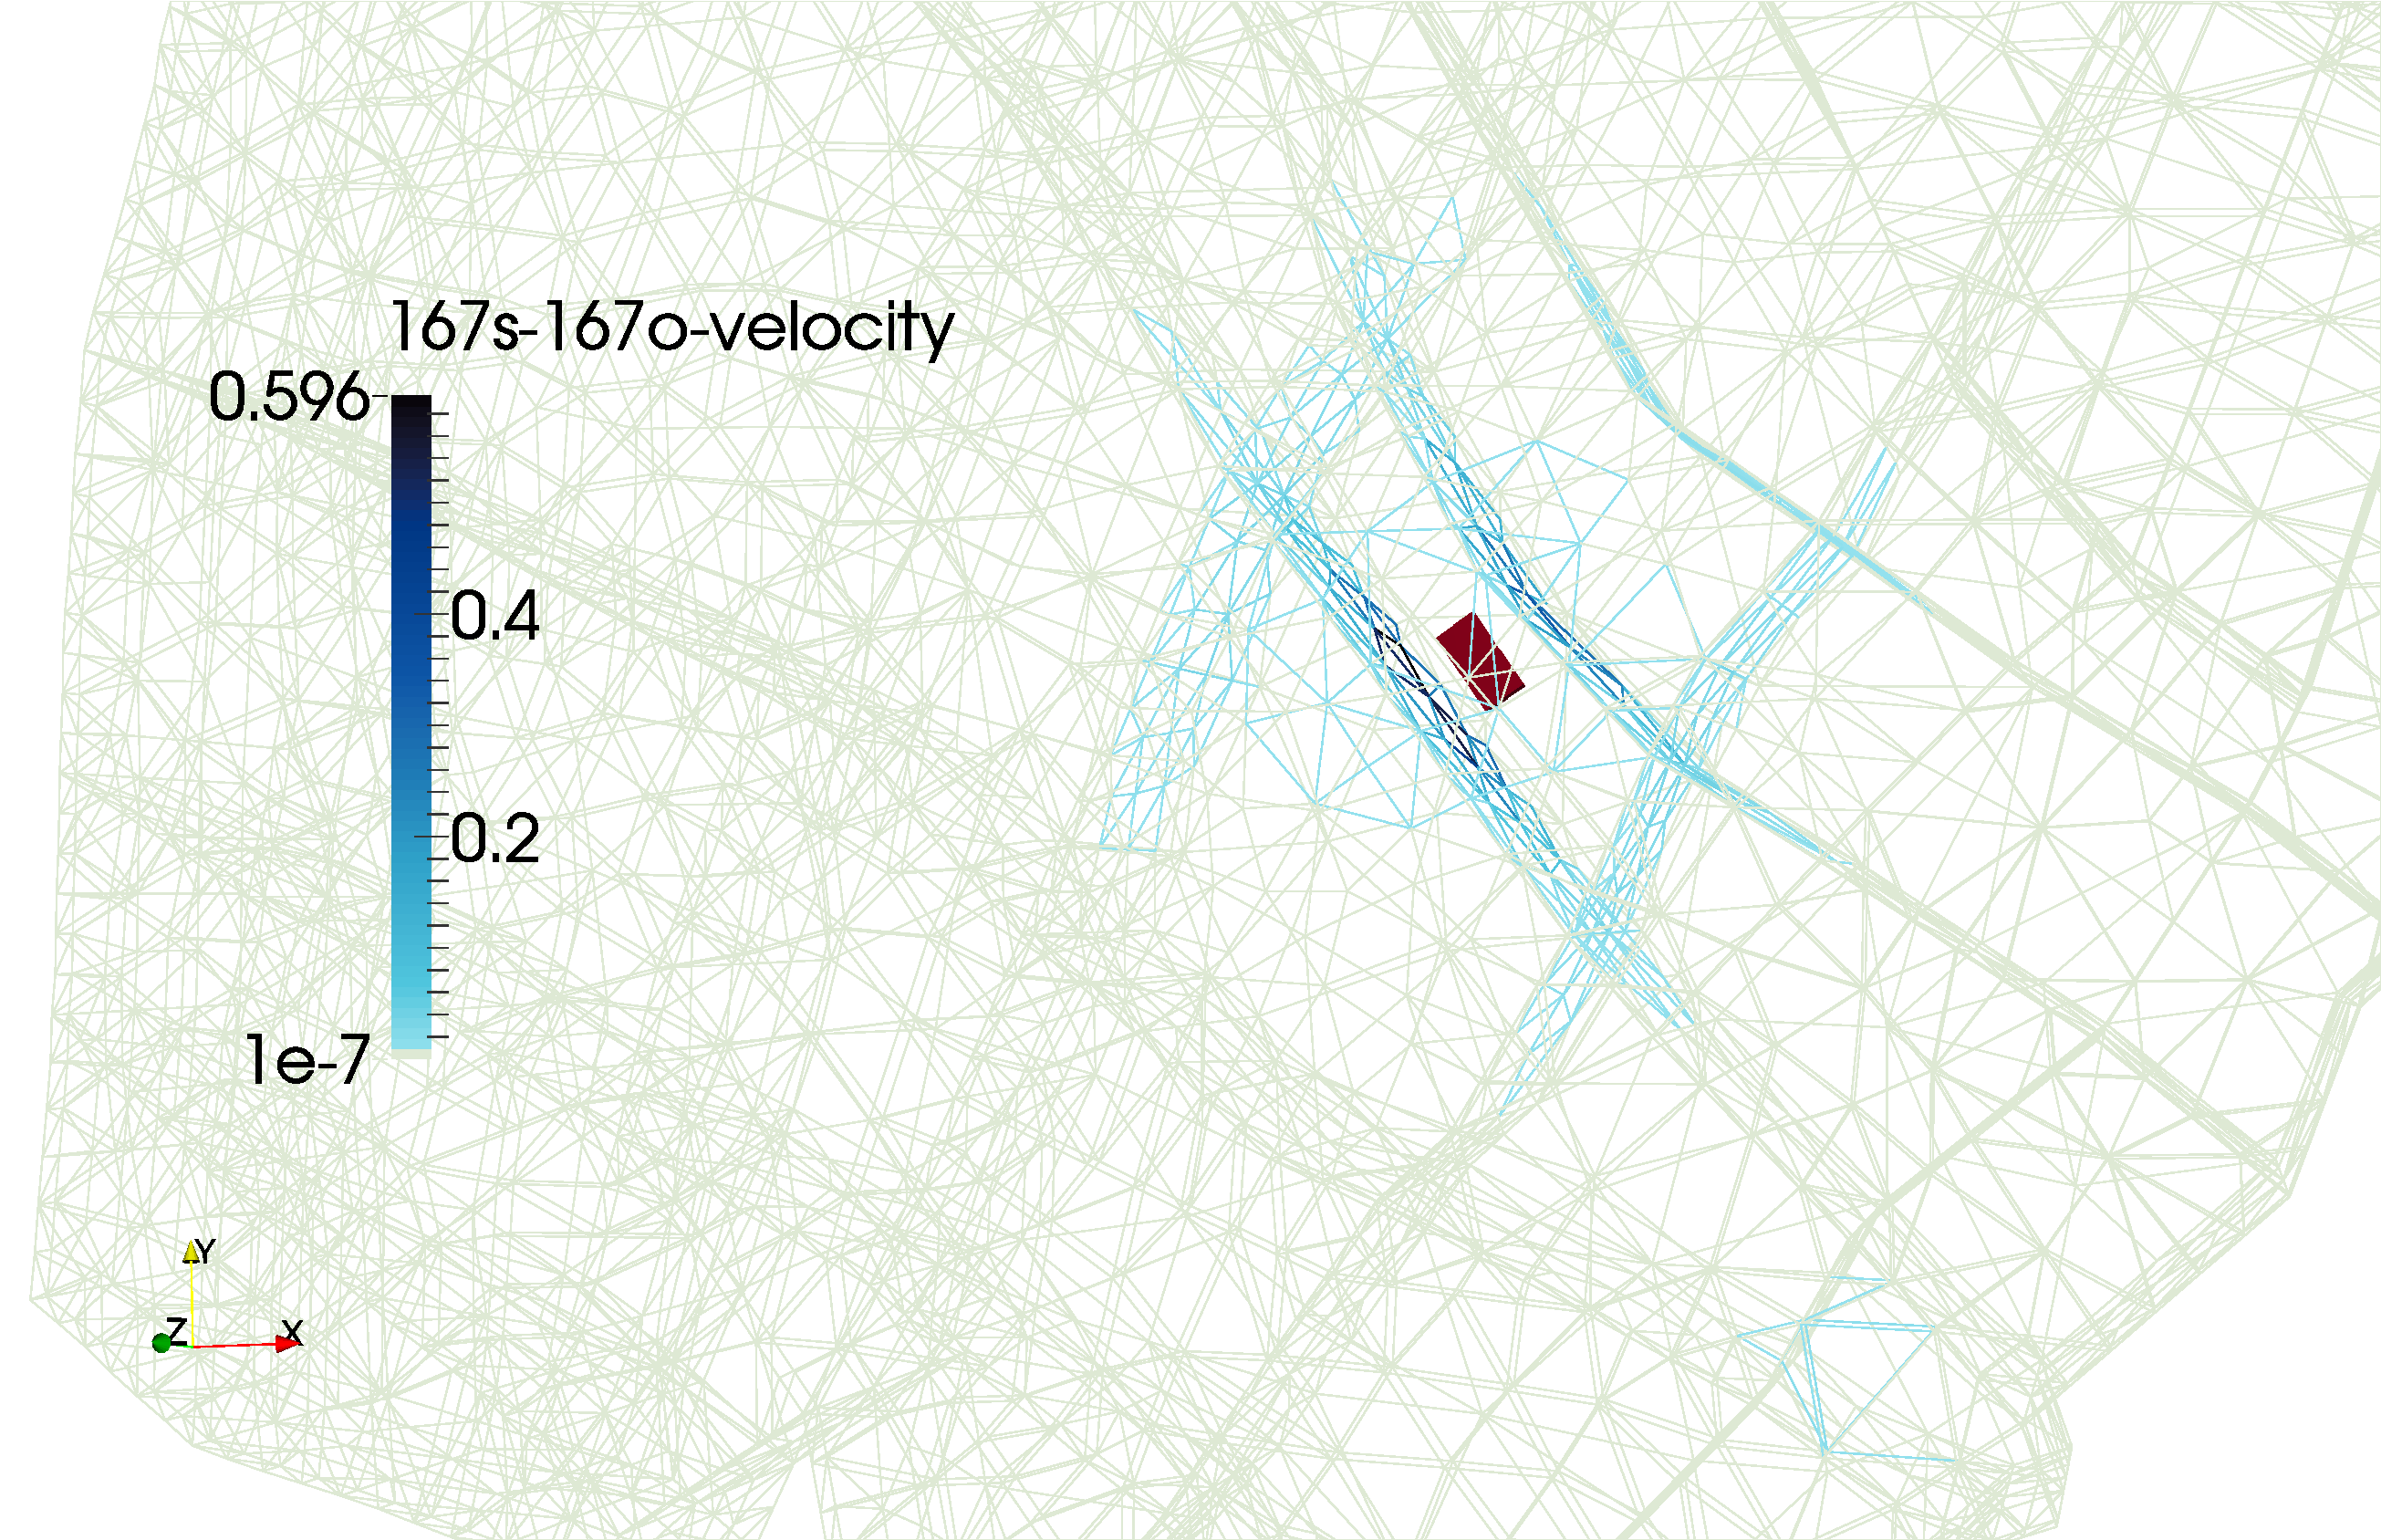
\includegraphics[width=0.60\textwidth]{tests_graphics/mel_167s-167_velocity.pdf}
        \caption{Difference in flow velocities between computation with Dirichlet BC and sources term (both computed in version 1.6.7). 
                 Red brick is the concentration source region.}
        \label{fig:bench_mel1}
\end{figure}
%
\begin{figure}[!h]
        \centering
        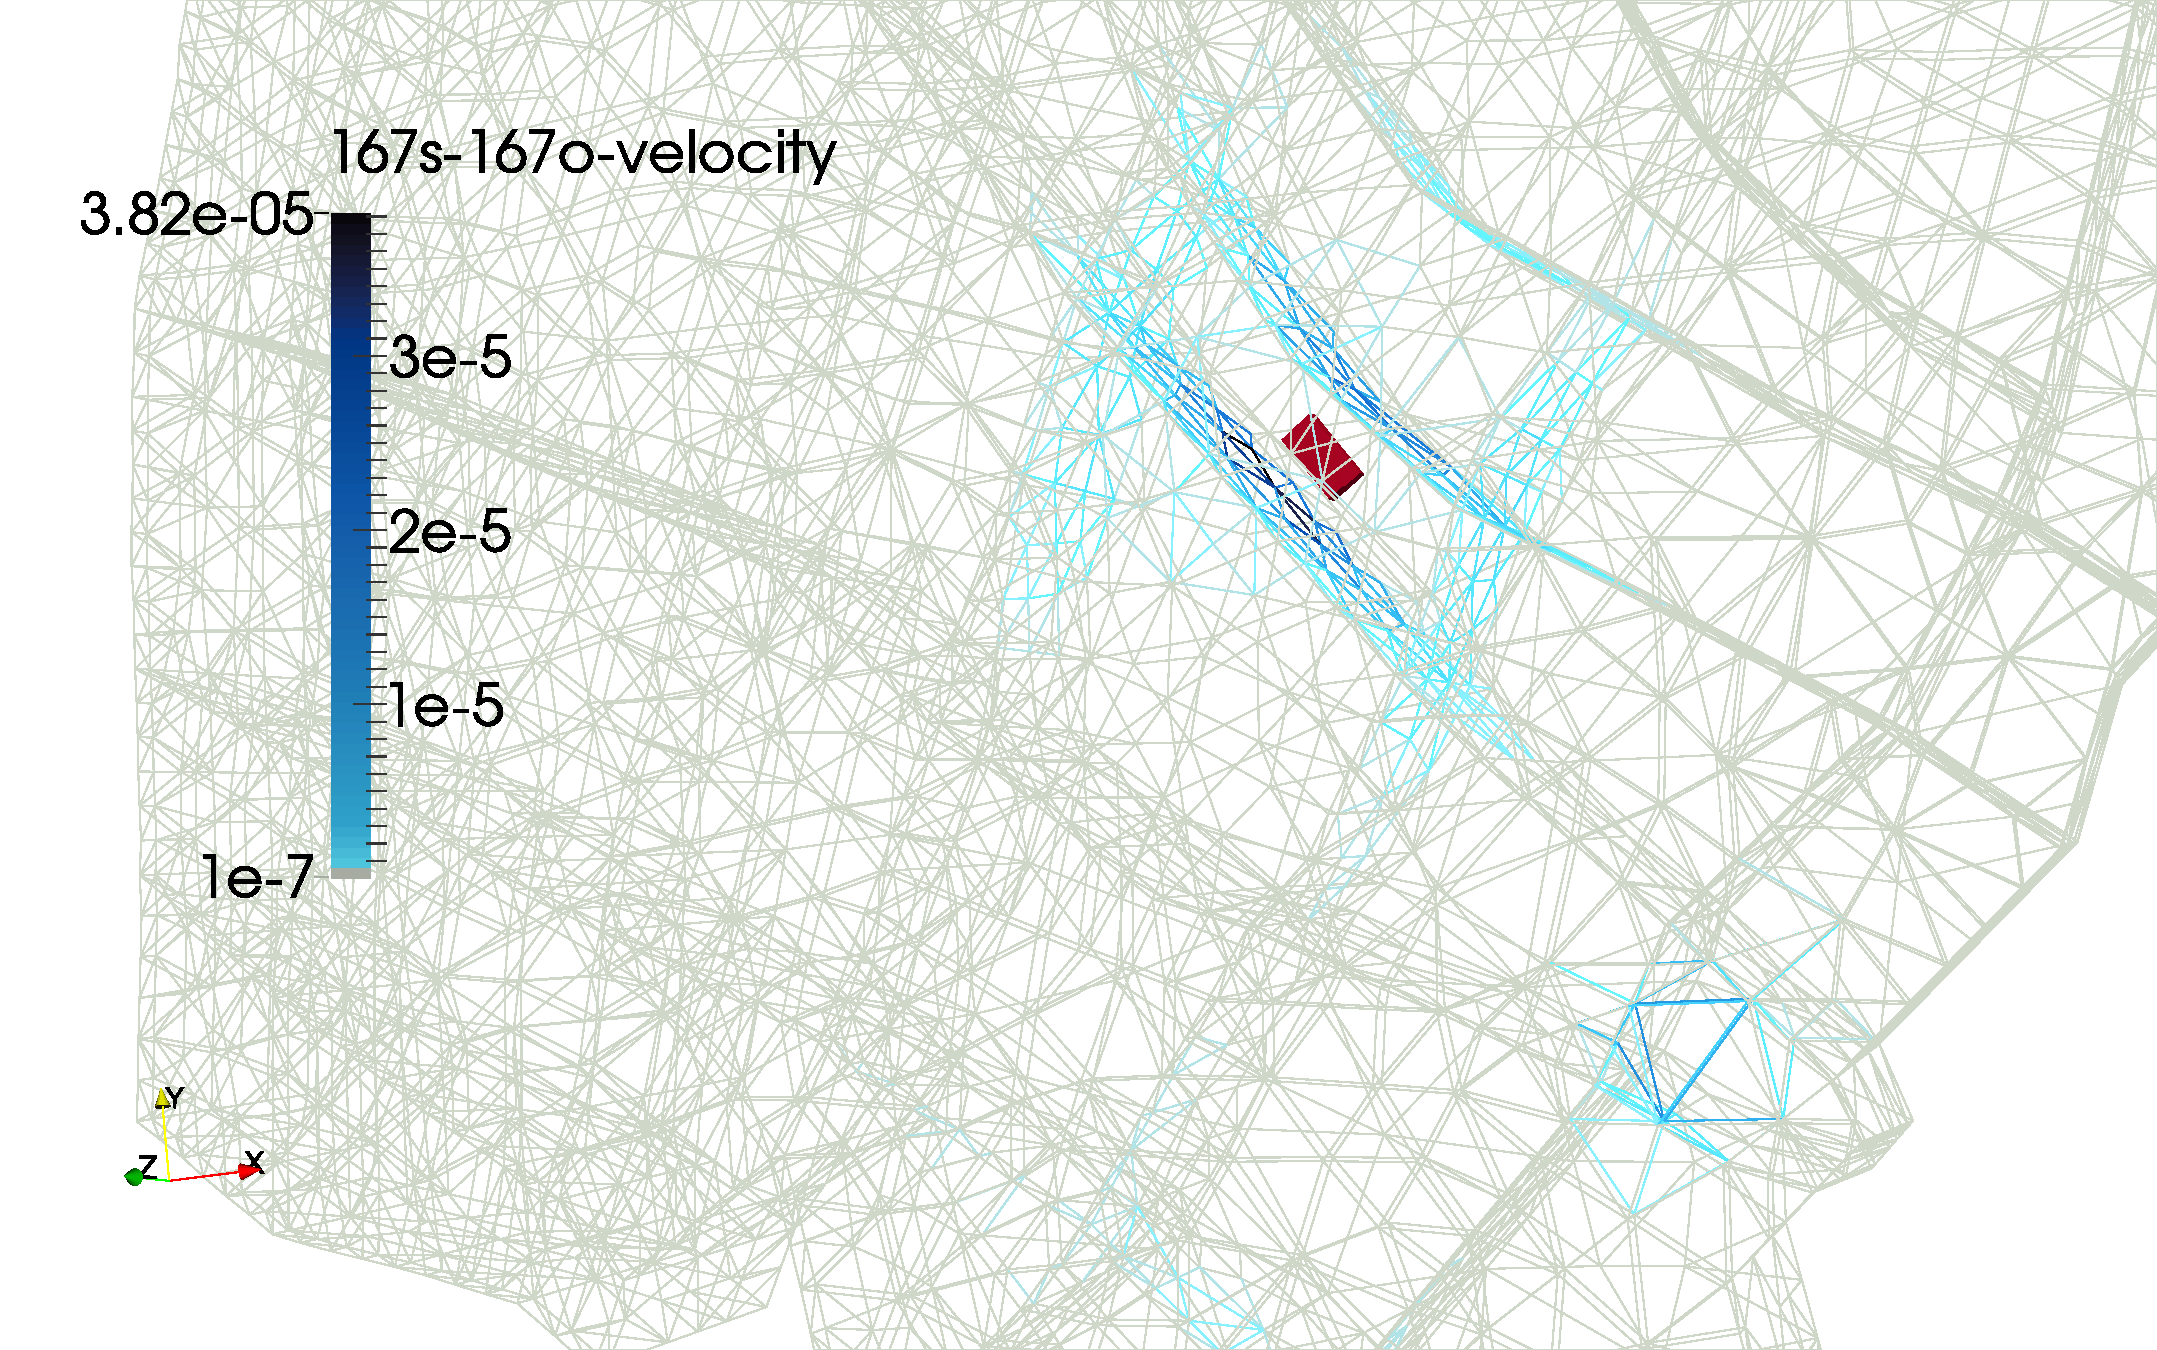
\includegraphics[width=0.60\textwidth]{tests_graphics/mel_167s-167o_velocity_equal.pdf}
        \caption{Difference in flow velocities between computation with new Dirichlet BC and sources term (both computed in version 1.6.7). 
                 Red brick is the concentration source region.}
        \label{fig:bench_mel2}
\end{figure}
%
\begin{figure}[!h]
        \centering
        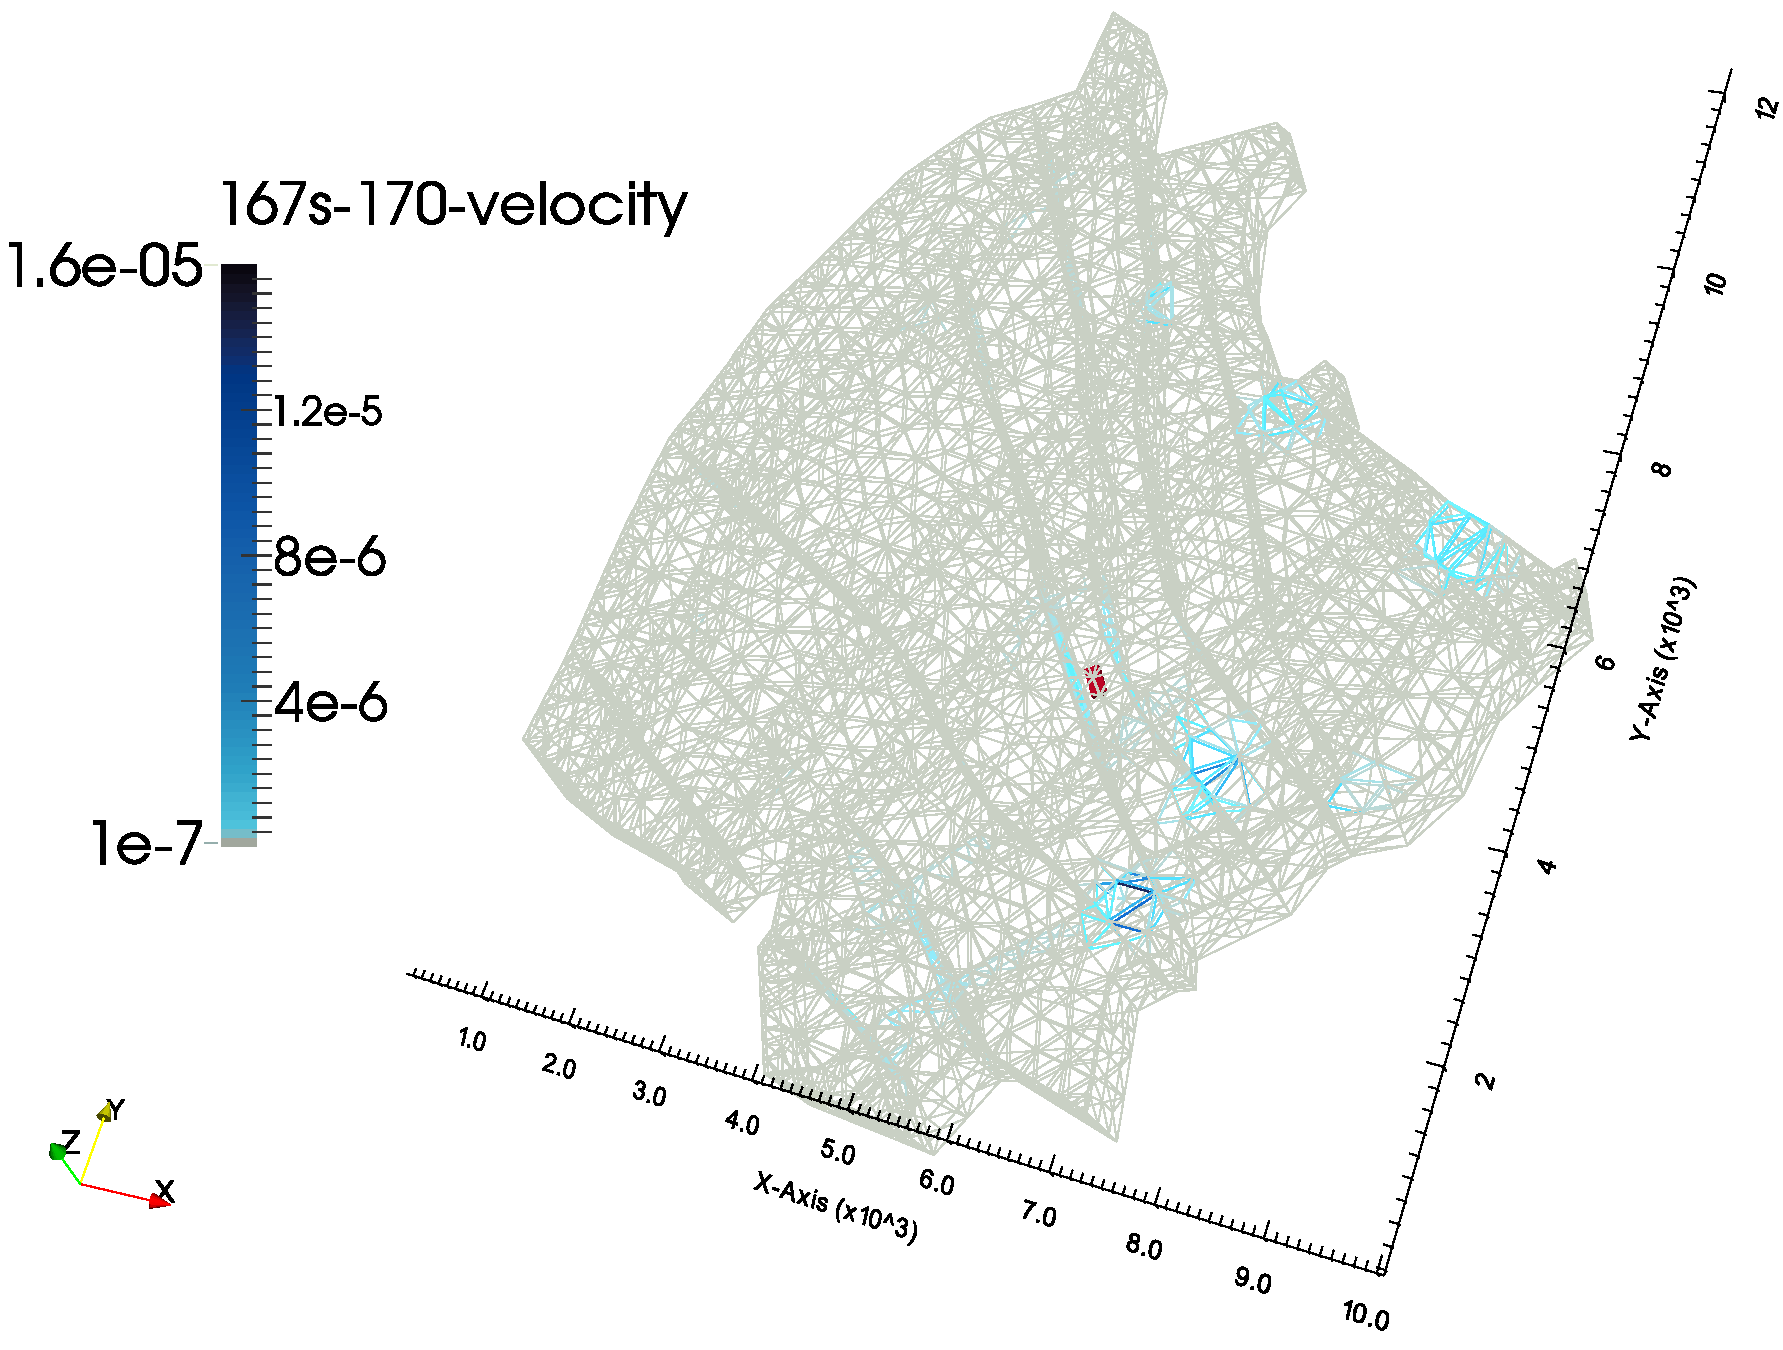
\includegraphics[width=0.75\textwidth]{tests_graphics/mel_167s-170_velocity_equal.pdf}
        \caption{Difference in flow velocities between solutions computed by versions 1.6.7 and 1.7.0 (with sources term).
                 Red brick is the concentration source region.}
        \label{fig:bench_mel5}
\end{figure}


In the figure \ref{fig:bench_mel1} we are showing the difference between the older solution (with Dirichlet BC 
prescribed in the area of deleted elements) and the solution in the compact area. We can see that there is a~considerable 
difference in the nearby area of deleted elements. In this case the reason is that somehow wrong values 
of pressure were prescribed as the Dirichlet BC. One can look for the difference into the raw output file 
where pressure and velocity on element sides can be found. The solutions in farther regions are considered equal 
with the precision of the solver $10^{-7}$.

To prove that the velocities are the same whether the source region is present in the mesh or not, we recalculated the flow and used the correct pressure values
for the Dirichlet boundary condition. The result is shown in the figure \ref{fig:bench_mel2} where the difference is much smaller.
The source of the difference comes most probably from the postprocessing where the velocities are computed from the pressure. 
The error of pressure computed by solver (in order of $10^{-7}$) can be increased by multiplication with the conductivity
which is larger than 1000 in some regions.


% \begin{figure}
%     \centering
%     \begin{subfigure}[b]{0.48\textwidth}
%         \centering
%         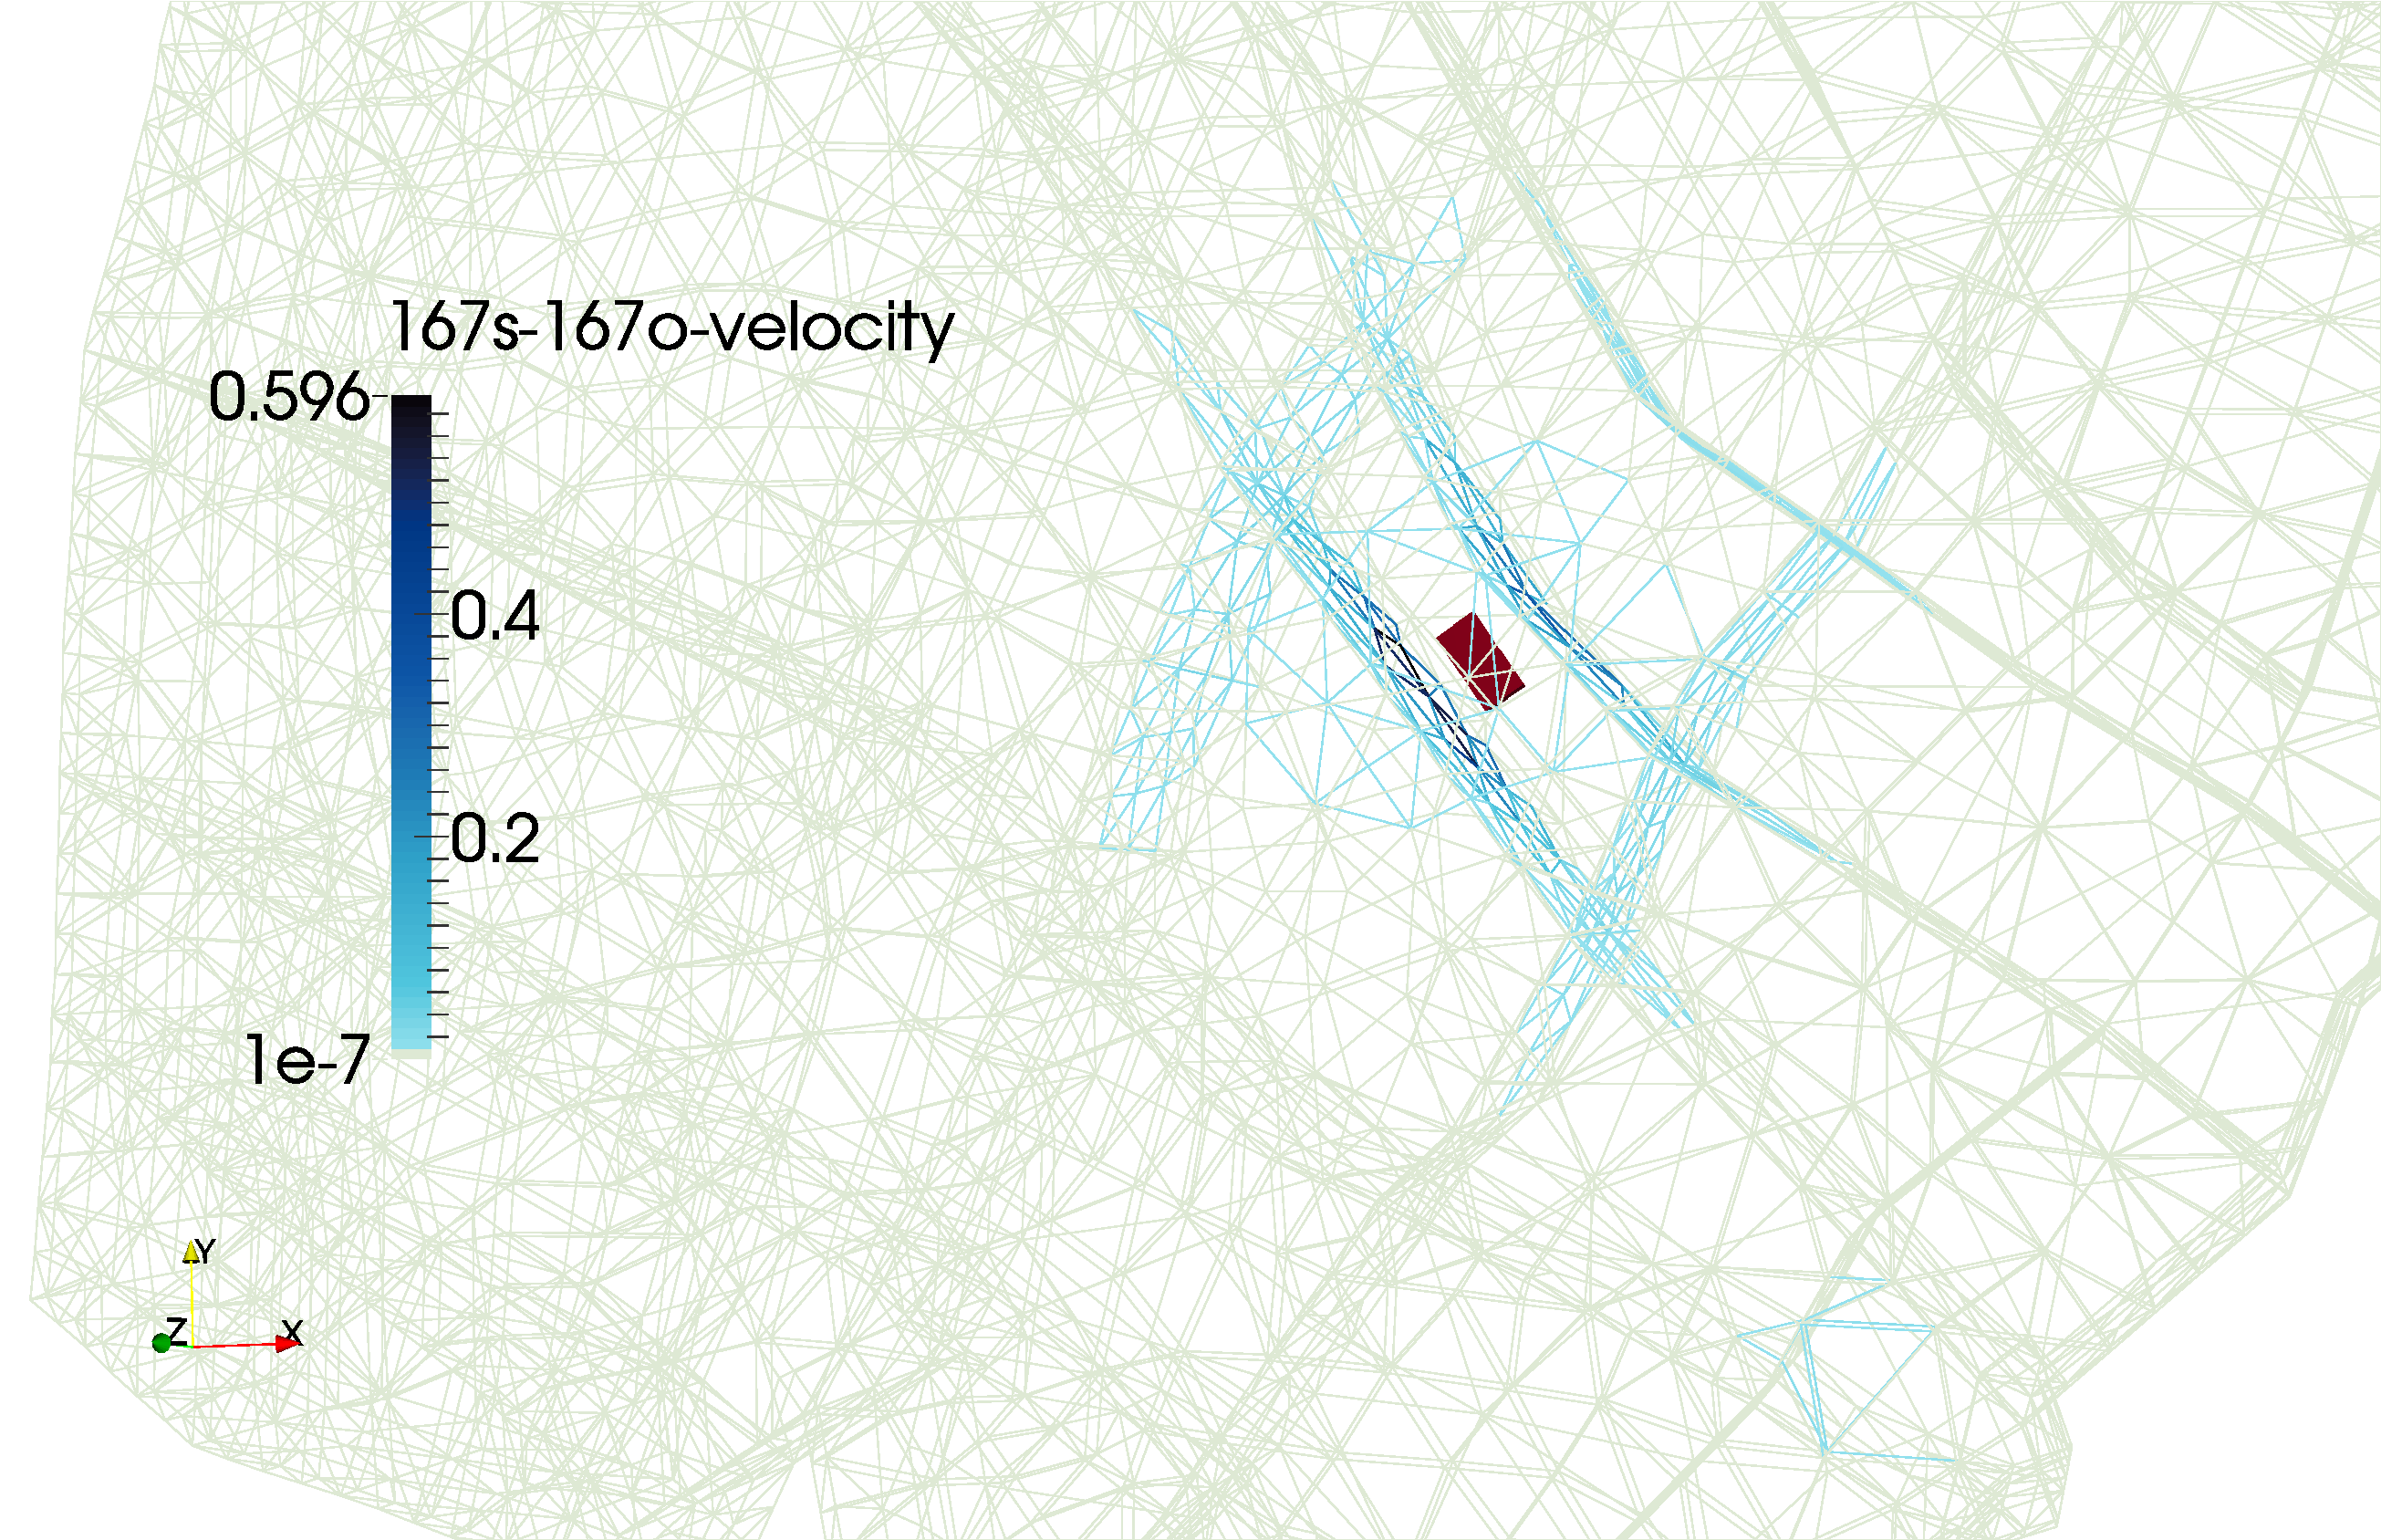
\includegraphics[width=\textwidth]{tests_graphics/mel_167s-167_velocity.pdf}
%         \caption{Elementwise pressure head and velocity field (triangles).}
%         \label{fig:bench_mel1}
%     \end{subfigure}
%     \begin{subfigure}[b]{0.48\textwidth}
%         \centering
%         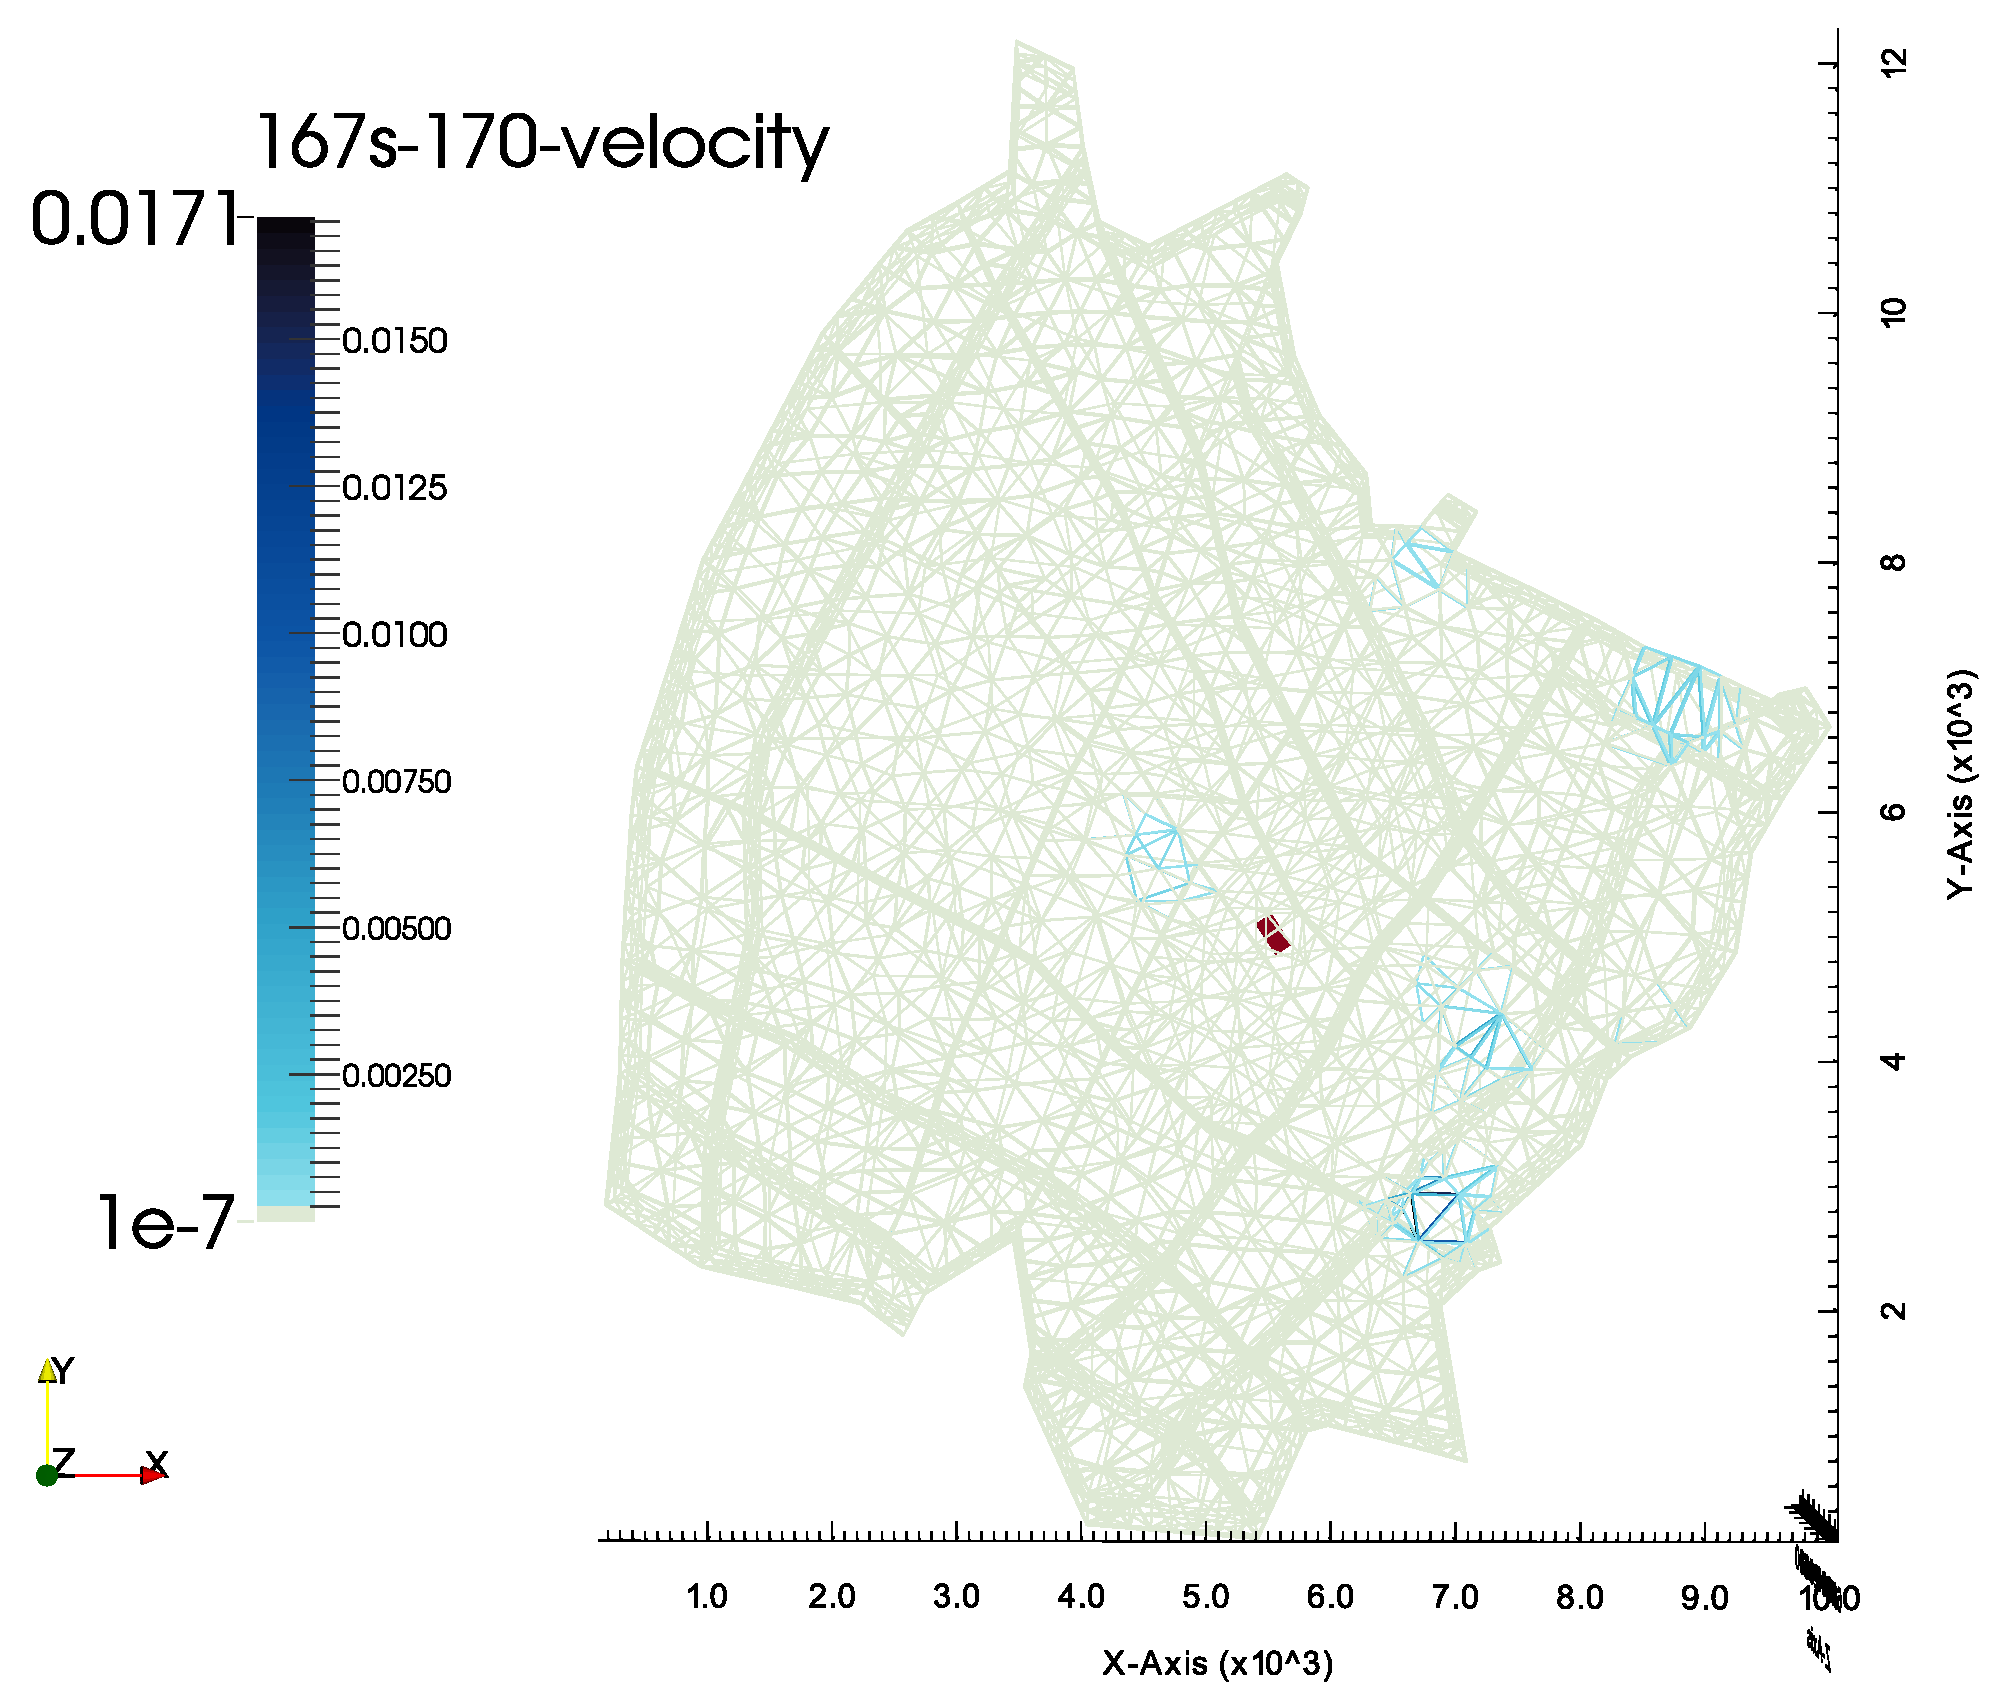
\includegraphics[width=\textwidth]{tests_graphics/mel_167s-170_velocity.pdf}
%         \caption{Elementwise pressure head and velocity field (triangles).}
%         \label{fig:bench_mel2}
%     \end{subfigure}
% \end{figure}

In the figure \ref{fig:bench_mel5} we also demonstrate small difference in water flow computed by versions 1.6.7 and 1.7.0. 
There are 5 areas where the difference is larger than the solver accuracy (set $10^{-7}$). This is caused again by 
postprocessing as we mentioned above.

\subsection{Transport}
The transport of the substance was computed over time period of $10^4$ years. In the figure \ref{fig:bench_mel3} we can see 
where the substance spread in concentration above $10^{-7}$~\unitss{1}{-3}{} which again corresponds to the solver accuracy.
We can compare the solutions computed by different versions in subfigures \ref{fig:bench_mel3a} to \ref{fig:bench_mel3c}.
The transport is caused only by convection so the velocities computed before are determining. As we can see in the figure 
\ref{fig:bench_mel1}, the difference in velocities is positive which means the velocities were smaller when the wrong Dirichlet 
boundary condition for flow was prescribed on the concentration source region. That is why the convectional transport is 
also slower in that case as we can observe in the figure \ref{fig:bench_mel3a}. 
The transport computed with source term prescribed is the same in both versions 1.6.7 and 1.7.0 as ilustrated in the figure
\ref{fig:bench_mel3b} and \ref{fig:bench_mel3c}. One can open Paraview state file to see that the difference in transport is in
order $10^{-7}$ corresponding again to the solver accuracy.

\begin{figure}[!h]
    \centering
    \begin{subfigure}[b]{0.3\textwidth}
        \centering
        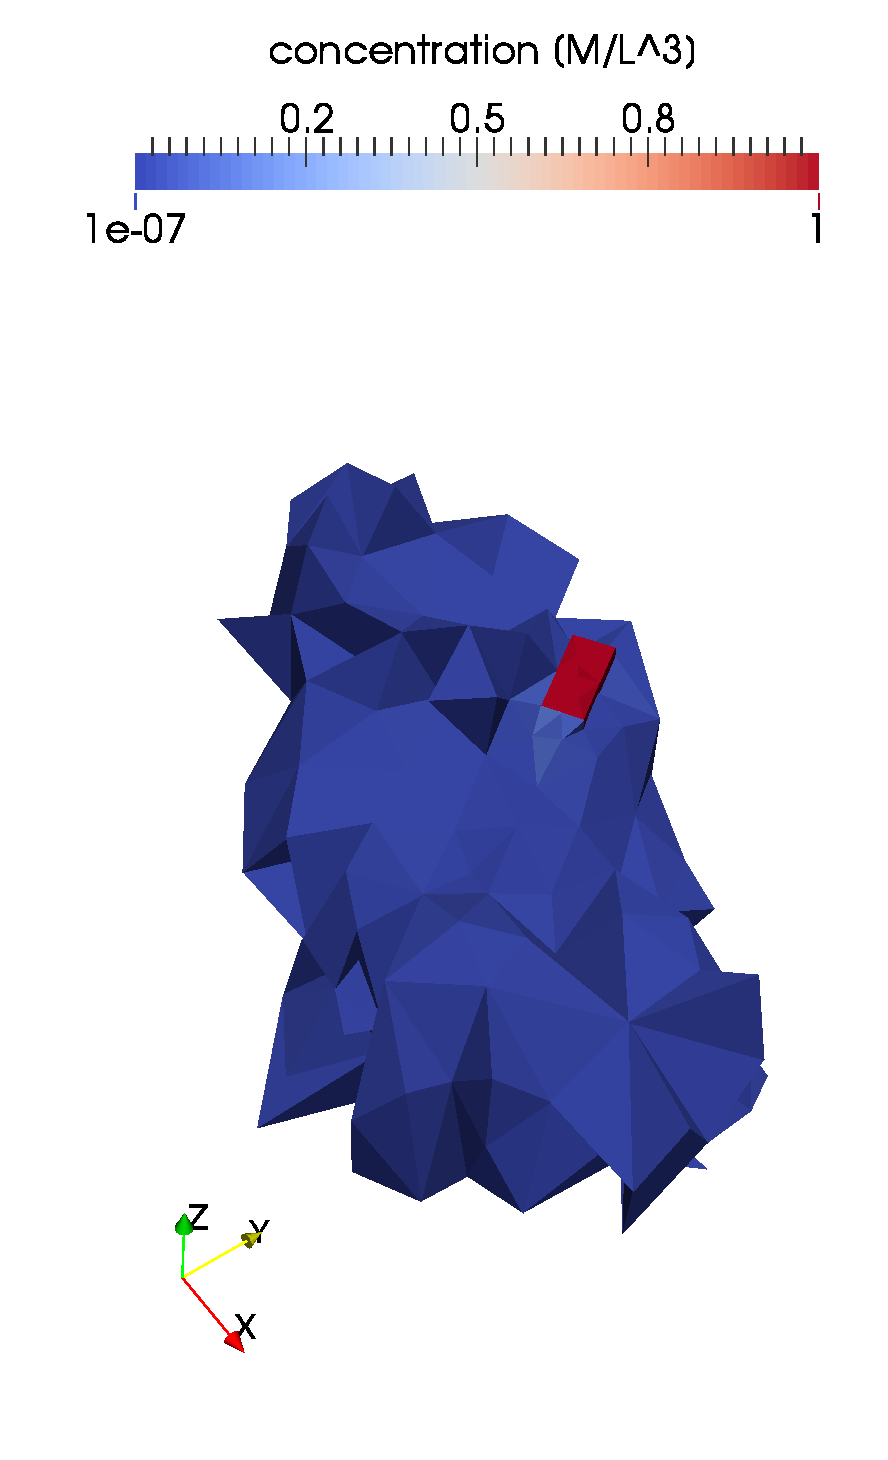
\includegraphics[width=\textwidth]{tests_graphics/mel_transport_end_167o.pdf}
        \caption{Program version 1.6.7, computed with Dirichlet BC.}
        \label{fig:bench_mel3a}
    \end{subfigure}
    ~
    \begin{subfigure}[b]{0.3\textwidth}
        \centering
        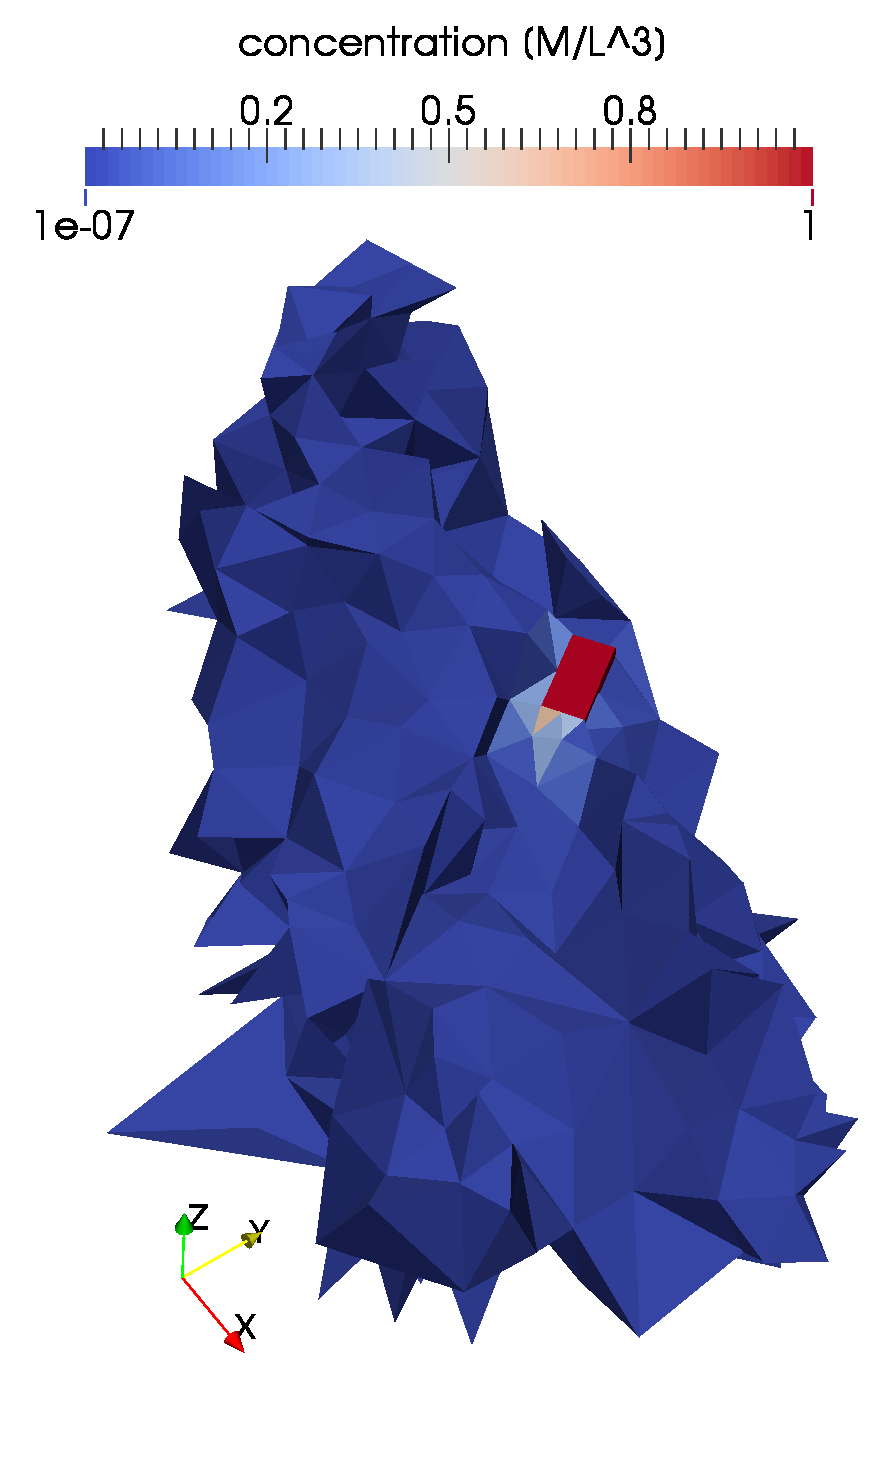
\includegraphics[width=\textwidth]{tests_graphics/mel_transport_end_167s.pdf}
        \caption{Program version 1.6.7, computed with source term prescribed.}
        \label{fig:bench_mel3b}
    \end{subfigure}
    ~
    \begin{subfigure}[b]{0.3\textwidth}
        \centering
        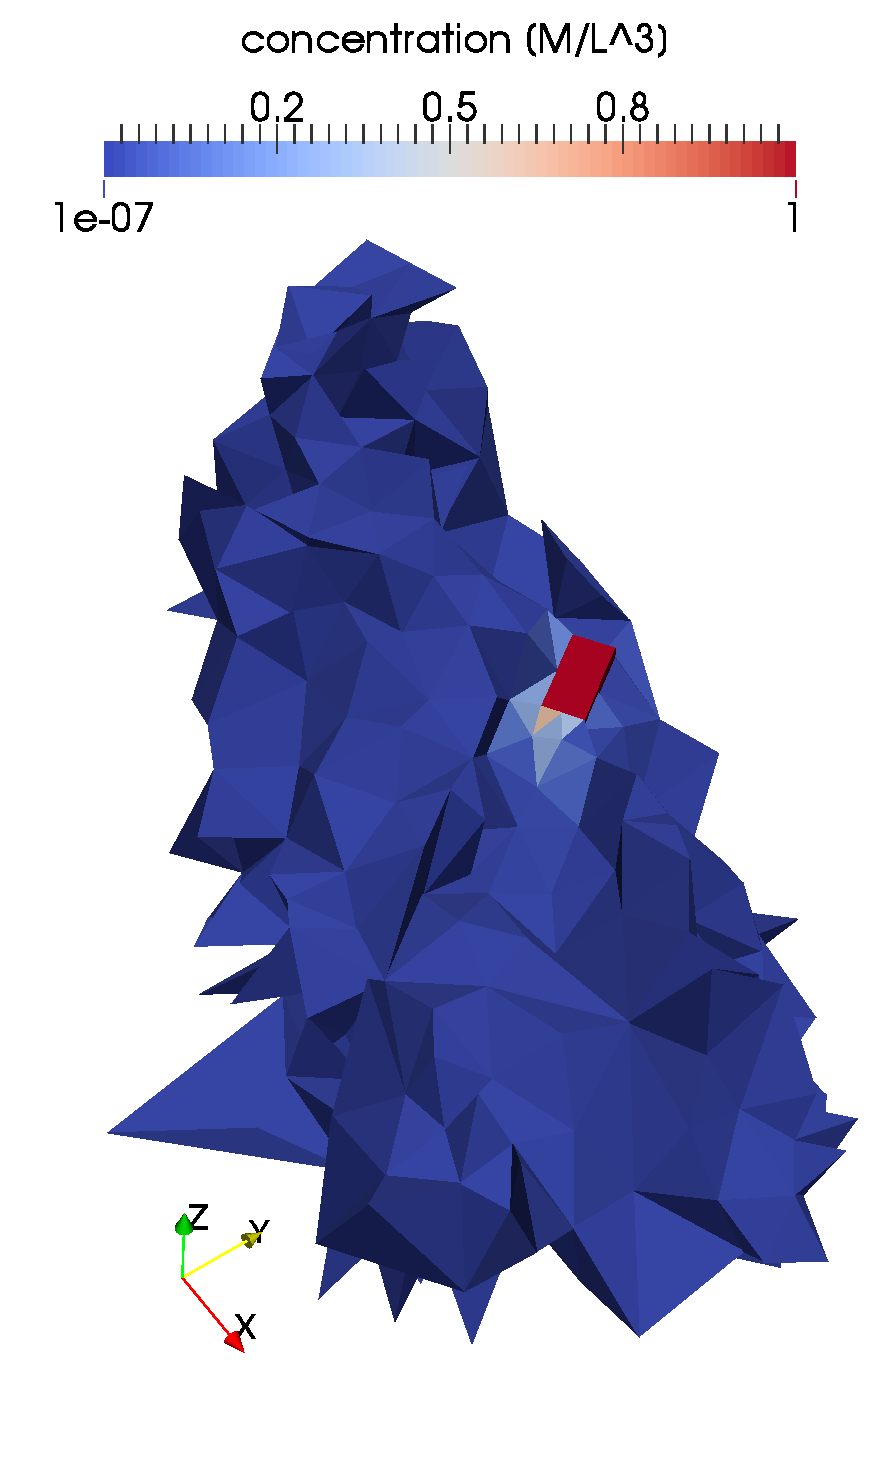
\includegraphics[width=\textwidth]{tests_graphics/mel_transport_end_170.pdf}
        \caption{Program version 1.7.0, computed with source term prescribed.}
        \label{fig:bench_mel3c}
    \end{subfigure}
    \caption{Concentration of the transported substance after $10^4$ years.}
    \label{fig:bench_mel3}
\end{figure}

Because the problem was originally computed on $10^6$ years, we show in figures \ref{fig:bench_mel4a} to \ref{fig:bench_mel4c} 
also the results of transport after this longer period.

\vfil

\textbf{Conclusion.} We can conclude that the results in all cases are the same with respect to the solver accuracy (both flow and transport) when 
the input files are made correctly. We would obtain the same results of transport in all three cases like shown in figures \ref{fig:bench_mel3b}, \ref{fig:bench_mel3c} and 
\ref{fig:bench_mel4b}, \ref{fig:bench_mel4c}. Comparing the solutions, pressure and velocity are equal when correct boundary condition values are applied. 
The transport can be defined both by Dirichlet boundary condition on the source region and by prescribing a source term on that region. 
We should mention that we used the source term in the form $F_S = \sigma_s(c_S-c)$, according to (\ref{eqn:transport_sources}).

\pagebreak

\begin{figure}[!h]
    \centering
    \begin{subfigure}[b]{0.3\textwidth}
        \centering
        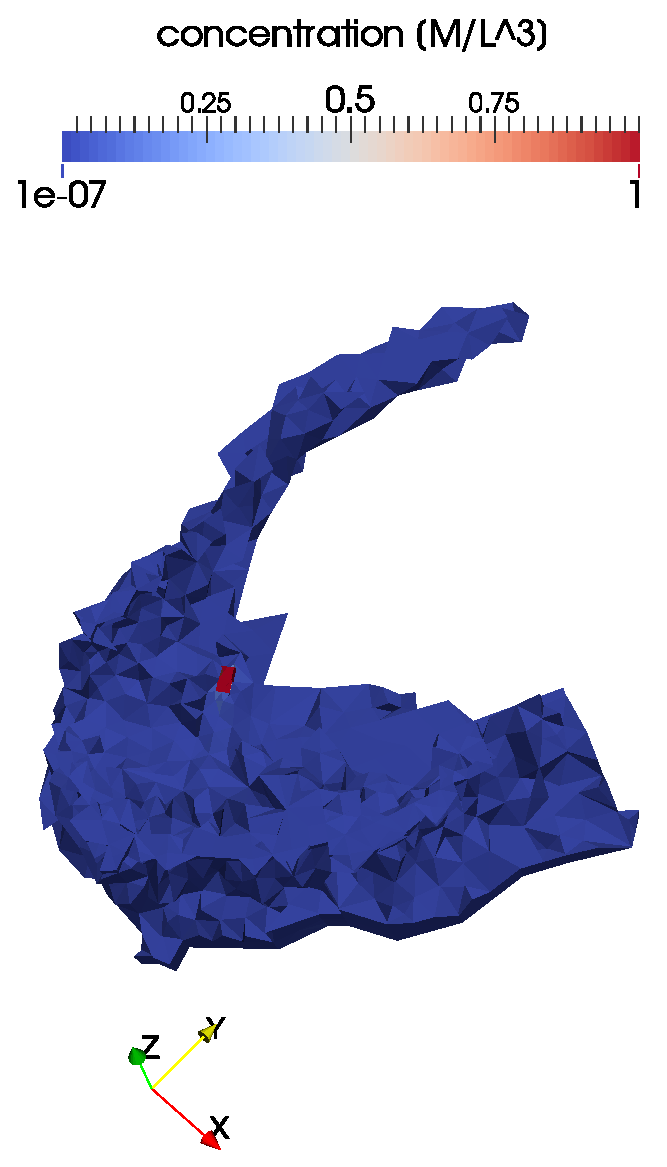
\includegraphics[width=\textwidth]{tests_graphics/mel_long_end_167o.pdf}
        \caption{Program version 1.6.7, computed with Dirichlet BC.}
        \label{fig:bench_mel4a}
    \end{subfigure}
    ~
    \begin{subfigure}[b]{0.3\textwidth}
        \centering
        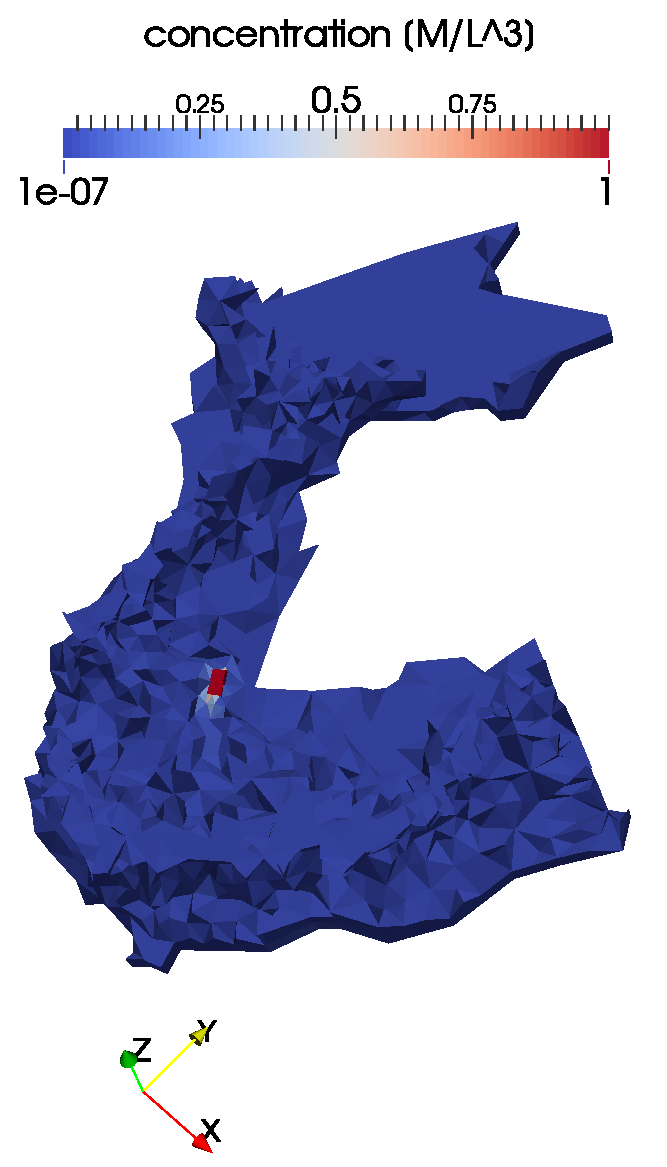
\includegraphics[width=\textwidth]{tests_graphics/mel_long_end_167s.pdf}
        \caption{Program version 1.6.7, computed with source term prescribed.}
        \label{fig:bench_mel4b}
    \end{subfigure}
    ~
    \begin{subfigure}[b]{0.3\textwidth}
        \centering
        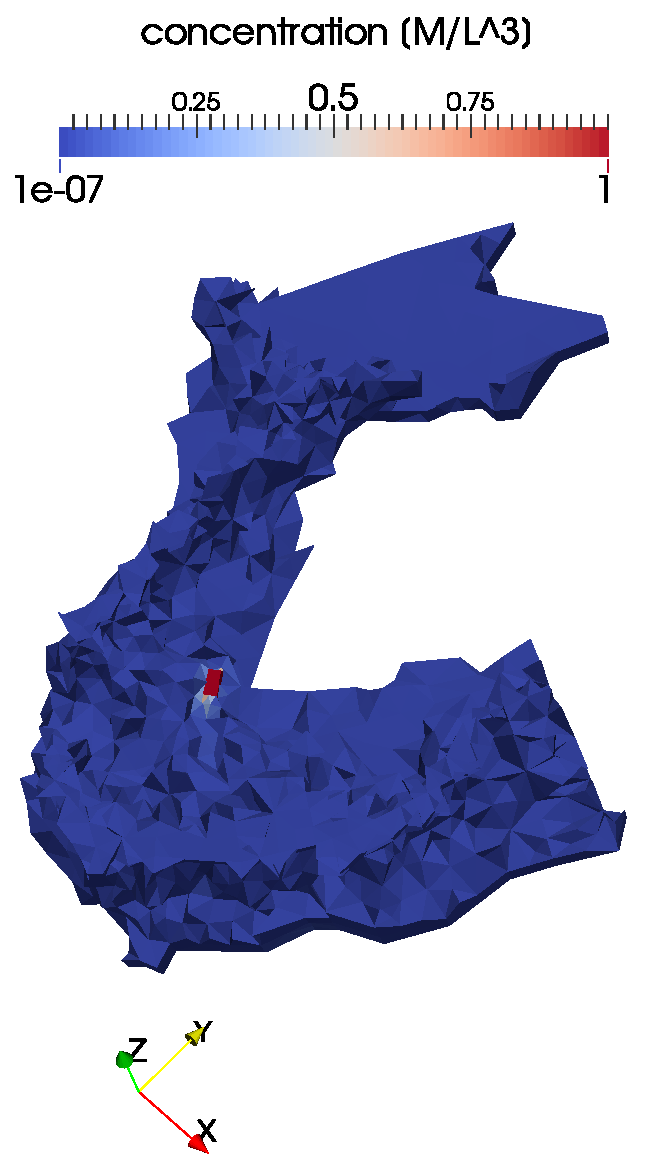
\includegraphics[width=\textwidth]{tests_graphics/mel_long_end_170.pdf}
        \caption{Program version 1.7.0, computed with source term prescribed.}
        \label{fig:bench_mel4c}
    \end{subfigure}
    \caption{Concentration of the transported substance after $10^6$ years.}
    \label{fig:bench_mel4}
\end{figure}


\emph{\textbf{Notice.} If user compares the solutions of transport computed in versions 1.6.7 and 1.7.0 in Paraview (or other SW)
be aware of a little bug in version 1.6.7 -- the transport steps are labeled only by numbers (1,2,3,...) not by the 
corresponding times. }

\subsection{Faced problems}
Several errors, bugs and problems on user side has arised while converting the 
input structure to version 1.7.0 and while doing profiling. The followings should be avoided in the future.

\begin{itemize}
  \item \textbf{Problem} of \verb'.mtr'. file. There are several versions of input material file for 
        different Melechov meshes. Regions that are not present in the mesh and quantities that are not used in
        the equations are all ignored in version 1.6.7. This can be very confusing when transforming the input
        for the newer version 1.7.0. Fortunately newer version provides feedback on this matter and writes
        warnings in log file.

  \item \textbf{Problem.} We described how concentration source can be prescribed by transport boundary condition above.
        To remove the elements from the mesh one used to only delete the neighborings in \verb'.ngh' file and then
        set the boundary condition on elements inside the bulk. This is not possible in newer versions and when using
        old \verb'.fbc' file with this kind of boundary condition, these  will be ignored.
  
  \item \textbf{Problem} with sigma parameter describing communication between fractures and volume.
        In version 1.6.7 this parameter is well hidden in \verb'.ngh' file as a tag at the end of
        lines. In version 1.7.0 one has to set this parameter in the bulk record of 2d and 1d regions 
        else the default value 1.0 will be used instead. A better physical model for estimation of this 
        parameter is beiing developed.

  \item \textbf{Problem} with solver accuracy. We found user mistakes in defining the solver accuracy in 
        old \verb'.ini' file. In version 1.6.7 one can use section \verb'Solver' to set solver accuracy,
        relative and absolute tolerance of the solver. Other way to set solver accuracy is to put it as
        input argument for Flow123d: \\
        \verb'          -ksp_atol 1.0e-10 -ksp_rtol 1.0e-10 -ksp_monitor'. \\
        These values are then passed to the PETSC solver.
        
  
%  \item \textbf{Problem} with (NOT) prescribing Dirichlet boudnary condition on the fractures. 

\end{itemize}


\chapter{Tutorials}\label{chapter:tutorials}
\section{Tutorials}
% define auxiliary command for tex source generated by pandoc
\providecommand{\tightlist}{%
  \setlength{\itemsep}{0pt}\setlength{\parskip}{0pt}}

\input 01_column.yaml.tex
\input 02_column_transport.yaml.tex
\input 03_tunnel.yaml.tex
\input 04_frac_diffusion.yaml.tex
\input 05_frac_sorption.yaml.tex
\input 06_frac_dualpor.yaml.tex
\input 07_heat.yaml.tex


\chapter{Main Input File Reference}
\label{chapter:input-tree-reference}
% support macros
This chapter contains generated reference to the main input file. Described types are ordered according to the 
deep first search of the input structure tree which somehow keep description of related types close to each other.
Interactive links allows passing through the tree structure in top-bottom manner. 

Ranges of arrays, integers and doubles use following notation: \verb'INT' for maximum of a signed 32-bit integer ($\approx 2.147\times 10^9$), 
\verb'UINT' for maximum of unsigned 32-bit integer ($\approx 4.295\times 10^9$), and
\verb'inf' for maximum of the double precision floating point number ($\approx1.798\times 10^{308}$). 
\pagebreak

% generated file

\begin{RecordType}{\HTRaised{IT::Root}{Root}}{}{}{\relax}{Root record of JSON input for Flow123d.}
\KeyItem{\hyperB{Root::problem}{problem}}{abstract type: \hyperlink{IT::Problem}{Problem}}{\textless\it obligatory\textgreater}{}{Simulation problem to be solved.}
\KeyItem{\hyperB{Root::pause-after-run}{pause\_after\_run}}{Bool}{false}{}{If true, the program will wait for key press before it terminates.}
\KeyItem{\hyperB{Root::output-streams}{output\_streams}}{Array  of record: \hyperlink{IT::OutputStream}{OutputStream}}{\textless\it optional\textgreater}{}{Array of formated output streams to open.}
\end{RecordType}

\begin{AbstractType}{\HTRaised{IT::Problem}{Problem}}{}{}{The root record of description of particular the problem to solve.}
\Descendant{\hyperlink{IT::SequentialCoupling}{SequentialCoupling}}
\end{AbstractType}

\begin{RecordType}{\HTRaised{IT::SequentialCoupling}{SequentialCoupling}}{\hyperlink{IT::Problem}{Problem}}{}{}{Record with data for a general sequential coupling.
}
\KeyItem{\hyperB{SequentialCoupling::TYPE}{TYPE}}{selection: Problem\_TYPE\_selection}{SequentialCoupling}{}{Sub-record selection.}
\KeyItem{\hyperB{SequentialCoupling::description}{description}}{String (generic)}{\textless\it optional\textgreater}{}{Short description of the solved problem.\\Is displayed in the main log, and possibly in other text output files.}
\KeyItem{\hyperB{SequentialCoupling::mesh}{mesh}}{record: \hyperlink{IT::Mesh}{Mesh}}{\textless\it obligatory\textgreater}{}{Computational mesh common to all equations.}
\KeyItem{\hyperB{SequentialCoupling::time}{time}}{record: \hyperlink{IT::TimeGovernor}{TimeGovernor}}{\textless\it optional\textgreater}{}{Simulation time frame and time step.}
\KeyItem{\hyperB{SequentialCoupling::primary-equation}{primary\_equation}}{abstract type: \hyperlink{IT::DarcyFlowMH}{DarcyFlowMH}}{\textless\it obligatory\textgreater}{}{Primary equation, have all data given.}
\KeyItem{\hyperB{SequentialCoupling::secondary-equation}{secondary\_equation}}{abstract type: \hyperlink{IT::Transport}{Transport}}{\textless\it optional\textgreater}{}{The equation that depends (the velocity field) on the result of the primary equation.}
\end{RecordType}

\begin{RecordType}{\HTRaised{IT::Mesh}{Mesh}}{}{}{\hyperlink{}{}}{Record with mesh related data.}
\KeyItem{\hyperB{Mesh::mesh-file}{mesh\_file}}{input file name}{\textless\it obligatory\textgreater}{\hyperlink{}{}}{Input file with mesh description.}
\KeyItem{\hyperB{Mesh::regions}{regions}}{Array  of record: \hyperlink{IT::Region}{Region}}{\textless\it optional\textgreater}{}{List of additional region definitions not contained in the mesh.}
\KeyItem{\hyperB{Mesh::sets}{sets}}{Array  of record: \hyperlink{IT::RegionSet}{RegionSet}}{\textless\it optional\textgreater}{}{List of region set definitions. There are three region sets implicitly defined:\\ALL (all regions of the mesh), BOUNDARY (all boundary regions), and BULK (all bulk regions)}
\KeyItem{\hyperB{Mesh::partitioning}{partitioning}}{record: \hyperlink{IT::Partition}{Partition}}{any\_neighboring}{}{Parameters of mesh partitioning algorithms.\\}
\end{RecordType}

\begin{RecordType}{\HTRaised{IT::Region}{Region}}{}{}{}{Definition of region of elements.}
\KeyItem{\hyperB{Region::name}{name}}{String (generic)}{\textless\it obligatory\textgreater}{}{Label (name) of the region. Has to be unique in one mesh.\\}
\KeyItem{\hyperB{Region::id}{id}}{Integer [0, ]}{\textless\it obligatory\textgreater}{}{The ID of the region to which you assign label.}
\KeyItem{\hyperB{Region::element-list}{element\_list}}{Array  of Integer [0, ]}{\textless\it optional\textgreater}{}{Specification of the region by the list of elements. This is not recomended}
\end{RecordType}

\begin{RecordType}{\HTRaised{IT::RegionSet}{RegionSet}}{}{}{}{Definition of one region set.}
\KeyItem{\hyperB{RegionSet::name}{name}}{String (generic)}{\textless\it obligatory\textgreater}{}{Unique name of the region set.}
\KeyItem{\hyperB{RegionSet::region-ids}{region\_ids}}{Array  of Integer [0, ]}{\textless\it optional\textgreater}{}{List of region ID numbers that has to be added to the region set.}
\KeyItem{\hyperB{RegionSet::region-labels}{region\_labels}}{Array  of String (generic)}{\textless\it optional\textgreater}{}{List of labels of the regions that has to be added to the region set.}
\KeyItem{\hyperB{RegionSet::union}{union}}{Array [2, 2] of String (generic)}{\textless\it optional\textgreater}{}{Defines region set as a union of given pair of sets. Overrides previous keys.}
\KeyItem{\hyperB{RegionSet::intersection}{intersection}}{Array [2, 2] of String (generic)}{\textless\it optional\textgreater}{}{Defines region set as an intersection of given pair of sets. Overrides previous keys.}
\KeyItem{\hyperB{RegionSet::difference}{difference}}{Array [2, 2] of String (generic)}{\textless\it optional\textgreater}{}{Defines region set as a difference of given pair of sets. Overrides previous keys.}
\end{RecordType}

\begin{RecordType}{\HTRaised{IT::Partition}{Partition}}{}{\hyperlink{Partition::graph-type}{graph\_type}}{}{Setting for various types of mesh partitioning.}
\KeyItem{\hyperB{Partition::tool}{tool}}{selection: \hyperlink{IT::PartTool}{PartTool}}{METIS}{}{Software package used for partitioning. See corresponding selection.}
\KeyItem{\hyperB{Partition::graph-type}{graph\_type}}{selection: \hyperlink{IT::GraphType}{GraphType}}{any\_neighboring}{}{Algorithm for generating graph and its weights from a multidimensional mesh.}
\end{RecordType}

\begin{SelectionType}{\HTRaised{IT::PartTool}{PartTool}}{Select the partitioning tool to use.}
\KeyItem{PETSc}{Use PETSc interface to various partitioning tools.}
\KeyItem{METIS}{Use direct interface to Metis.}
\end{SelectionType}

\begin{SelectionType}{\HTRaised{IT::GraphType}{GraphType}}{Different algorithms to make the sparse graph with weighted edges
from the multidimensional mesh. Main difference is dealing with 
neighborings of elements of different dimension.}
\KeyItem{any\_neighboring}{Add edge for any pair of neighboring elements.}
\KeyItem{any\_wight\_lower\_dim\_cuts}{Same as before and assign higher weight to cuts of lower dimension in order to make them stick to one face.}
\KeyItem{same\_dimension\_neghboring}{Add edge for any pair of neighboring elements of same dimension (bad for matrix multiply).}
\end{SelectionType}

\begin{RecordType}{\HTRaised{IT::TimeGovernor}{TimeGovernor}}{}{}{}{Setting of the simulation time. (can be specific to one eqaution)}
\KeyItem{\hyperB{TimeGovernor::start-time}{start\_time}}{Double }{0.0}{}{Start time of the simulation.}
\KeyItem{\hyperB{TimeGovernor::end-time}{end\_time}}{Double }{\textless\it obligatory\textgreater}{}{End time of the simulation.}
\KeyItem{\hyperB{TimeGovernor::init-dt}{init\_dt}}{Double [0, ]}{\textless\it optional\textgreater}{}{Initial guess for the time step. The time step is fixed if hard time step limits are not set.}
\KeyItem{\hyperB{TimeGovernor::min-dt}{min\_dt}}{Double [0, ]}{"Machine precision or 'init\_dt' if specified"}{}{Hard lower limit for the time step.}
\KeyItem{\hyperB{TimeGovernor::max-dt}{max\_dt}}{Double [0, ]}{"Whole time of the simulation or 'init\_dt' if specified"}{}{Hard upper limit for the time step.}
\end{RecordType}

\begin{AbstractType}{\HTRaised{IT::DarcyFlowMH}{DarcyFlowMH}}{}{}{Mixed-Hybrid  solver for saturated Darcy flow.}
\Descendant{\hyperlink{IT::Steady-MH}{Steady\_MH}}
\Descendant{\hyperlink{IT::Unsteady-MH}{Unsteady\_MH}}
\Descendant{\hyperlink{IT::Unsteady-LMH}{Unsteady\_LMH}}
\end{AbstractType}

\begin{RecordType}{\HTRaised{IT::Steady-MH}{Steady\_MH}}{\hyperlink{IT::DarcyFlowMH}{DarcyFlowMH}}{}{}{Mixed-Hybrid  solver for STEADY saturated Darcy flow.}
\KeyItem{\hyperB{Steady-MH::TYPE}{TYPE}}{selection: DarcyFlowMH\_TYPE\_selection}{Steady\_MH}{}{Sub-record selection.}
\KeyItem{\hyperB{Steady-MH::n-schurs}{n\_schurs}}{Integer [0, 2]}{2}{}{Number of Schur complements to perform when solving MH sytem.}
\KeyItem{\hyperB{Steady-MH::solver}{solver}}{abstract type: \hyperlink{IT::Solver}{Solver}}{\textless\it obligatory\textgreater}{}{Linear solver for MH problem.}
\KeyItem{\hyperB{Steady-MH::output}{output}}{record: \hyperlink{IT::DarcyMHOutput}{DarcyMHOutput}}{\textless\it obligatory\textgreater}{}{Parameters of output form MH module.}
\KeyItem{\hyperB{Steady-MH::mortar-method}{mortar\_method}}{selection: \hyperlink{IT::MH-MortarMethod}{MH\_MortarMethod}}{None}{}{Method for coupling Darcy flow between dimensions.}
\KeyItem{\hyperB{Steady-MH::bc-data}{bc\_data}}{Array  of record: \hyperlink{IT::DarcyFlowMH-Steady-BoundaryData}{DarcyFlowMH\_Steady\_BoundaryData}}{\textless\it obligatory\textgreater}{}{}
\KeyItem{\hyperB{Steady-MH::bulk-data}{bulk\_data}}{Array  of record: \hyperlink{IT::DarcyFlowMH-Steady-BulkData}{DarcyFlowMH\_Steady\_BulkData}}{\textless\it obligatory\textgreater}{}{}
\end{RecordType}

\begin{AbstractType}{\HTRaised{IT::Solver}{Solver}}{}{}{Solver setting.}
\Descendant{\hyperlink{IT::Petsc}{Petsc}}
\Descendant{\hyperlink{IT::Bddc}{Bddc}}
\end{AbstractType}

\begin{RecordType}{\HTRaised{IT::Petsc}{Petsc}}{\hyperlink{IT::Solver}{Solver}}{}{}{Solver setting.}
\KeyItem{\hyperB{Petsc::TYPE}{TYPE}}{selection: Solver\_TYPE\_selection}{Petsc}{}{Sub-record selection.}
\KeyItem{\hyperB{Petsc::a-tol}{a\_tol}}{Double [0, ]}{1.0e-9}{}{Absolute residual tolerance.}
\KeyItem{\hyperB{Petsc::r-tol}{r\_tol}}{Double [0, 1]}{1.0e-7}{}{Relative residual tolerance (to initial error).}
\KeyItem{\hyperB{Petsc::max-it}{max\_it}}{Integer [0, ]}{10000}{}{Maximum number of outer iterations of the linear solver.}
\KeyItem{\hyperB{Petsc::options}{options}}{String (generic)}{}{}{Options passed to the petsc instead of default setting.}
\end{RecordType}

\begin{RecordType}{\HTRaised{IT::Bddc}{Bddc}}{\hyperlink{IT::Solver}{Solver}}{}{}{Solver setting.}
\KeyItem{\hyperB{Bddc::TYPE}{TYPE}}{selection: Solver\_TYPE\_selection}{Bddc}{}{Sub-record selection.}
\KeyItem{\hyperB{Bddc::a-tol}{a\_tol}}{Double [0, ]}{1.0e-9}{}{Absolute residual tolerance.}
\KeyItem{\hyperB{Bddc::r-tol}{r\_tol}}{Double [0, 1]}{1.0e-7}{}{Relative residual tolerance (to initial error).}
\KeyItem{\hyperB{Bddc::max-it}{max\_it}}{Integer [0, ]}{10000}{}{Maximum number of outer iterations of the linear solver.}
\end{RecordType}

\begin{RecordType}{\HTRaised{IT::DarcyMHOutput}{DarcyMHOutput}}{}{}{}{Parameters of MH output.}
\KeyItem{\hyperB{DarcyMHOutput::save-step}{save\_step}}{Double [0, ]}{1.0}{}{Regular step between MH outputs.}
\KeyItem{\hyperB{DarcyMHOutput::output-stream}{output\_stream}}{record: \hyperlink{IT::OutputStream}{OutputStream}}{\textless\it obligatory\textgreater}{}{Parameters of output stream.}
\KeyItem{\hyperB{DarcyMHOutput::velocity-p0}{velocity\_p0}}{String (generic)}{\textless\it optional\textgreater}{}{Output stream for P0 approximation of the velocity field.}
\KeyItem{\hyperB{DarcyMHOutput::pressure-p0}{pressure\_p0}}{String (generic)}{\textless\it optional\textgreater}{}{Output stream for P0 approximation of the pressure field.}
\KeyItem{\hyperB{DarcyMHOutput::pressure-p1}{pressure\_p1}}{String (generic)}{\textless\it optional\textgreater}{}{Output stream for P1 approximation of the pressure field.}
\KeyItem{\hyperB{DarcyMHOutput::piezo-head-p0}{piezo\_head\_p0}}{String (generic)}{\textless\it optional\textgreater}{}{Output stream for P0 approximation of the piezometric head field.}
\KeyItem{\hyperB{DarcyMHOutput::balance-output}{balance\_output}}{output file name}{water\_balance.txt}{}{Output file for water balance table.}
\KeyItem{\hyperB{DarcyMHOutput::subdomains}{subdomains}}{String (generic)}{\textless\it optional\textgreater}{}{Output stream for subdomain indices (partitioning of mesh elements) used by DarcyFlow module.}
\KeyItem{\hyperB{DarcyMHOutput::raw-flow-output}{raw\_flow\_output}}{output file name}{\textless\it optional\textgreater}{}{Output file with raw data form MH module.}
\end{RecordType}

\begin{RecordType}{\HTRaised{IT::OutputStream}{OutputStream}}{}{}{}{Parameters of output.}
\KeyItem{\hyperB{OutputStream::name}{name}}{String (generic)}{\textless\it obligatory\textgreater}{}{The name of this stream. Used to reference the output stream.}
\KeyItem{\hyperB{OutputStream::file}{file}}{output file name}{\textless\it obligatory\textgreater}{}{File path to the connected output file.}
\KeyItem{\hyperB{OutputStream::format}{format}}{abstract type: \hyperlink{IT::OutputFormat}{OutputFormat}}{\textless\it optional\textgreater}{}{Format of output stream and possible parameters.}
\end{RecordType}

\begin{AbstractType}{\HTRaised{IT::OutputFormat}{OutputFormat}}{}{}{Format of output stream and possible parameters.}
\Descendant{\hyperlink{IT::vtk}{vtk}}
\Descendant{\hyperlink{IT::gmsh}{gmsh}}
\end{AbstractType}

\begin{RecordType}{\HTRaised{IT::vtk}{vtk}}{\hyperlink{IT::OutputFormat}{OutputFormat}}{}{}{Parameters of vtk output format.}
\KeyItem{\hyperB{vtk::TYPE}{TYPE}}{selection: OutputFormat\_TYPE\_selection}{vtk}{}{Sub-record selection.}
\KeyItem{\hyperB{vtk::variant}{variant}}{selection: \hyperlink{IT::VTK variant (ascii or binary)}{VTK variant (ascii or binary)}}{ascii}{}{Variant of output stream file format.}
\KeyItem{\hyperB{vtk::parallel}{parallel}}{Bool}{false}{}{Parallel or serial version of file format.}
\KeyItem{\hyperB{vtk::compression}{compression}}{selection: \hyperlink{IT::Type of compression of VTK file format}{Type of compression of VTK file format}}{none}{}{Compression used in output stream file format.}
\end{RecordType}

\begin{SelectionType}{\HTRaised{IT::VTK variant (ascii or binary)}{VTK variant (ascii or binary)}}{}
\KeyItem{ascii}{ASCII variant of VTK file format}
\KeyItem{binary}{Binary variant of VTK file format (not supported yet)}
\end{SelectionType}

\begin{SelectionType}{\HTRaised{IT::Type of compression of VTK file format}{Type of compression of VTK file format}}{}
\KeyItem{none}{Data in VTK file format are not compressed}
\KeyItem{zlib}{Data in VTK file format are compressed using zlib (not supported yet)}
\end{SelectionType}

\begin{RecordType}{\HTRaised{IT::gmsh}{gmsh}}{\hyperlink{IT::OutputFormat}{OutputFormat}}{}{}{Parameters of gmsh output format.}
\KeyItem{\hyperB{gmsh::TYPE}{TYPE}}{selection: OutputFormat\_TYPE\_selection}{gmsh}{}{Sub-record selection.}
\end{RecordType}

\begin{SelectionType}{\HTRaised{IT::MH-MortarMethod}{MH\_MortarMethod}}{}
\KeyItem{None}{Mortar space: P0 on elements of lower dimension.}
\KeyItem{P0}{Mortar space: P0 on elements of lower dimension.}
\KeyItem{P1}{Mortar space: P1 on intersections, using non-conforming pressures.}
\end{SelectionType}

\begin{RecordType}{\HTRaised{IT::DarcyFlowMH-Steady-BoundaryData}{DarcyFlowMH\_Steady\_BoundaryData}}{}{}{}{Record to set BOUNDARY fields of the equation 'DarcyFlowMH\_Steady'.
The fields are set only on the domain specified by one of the keys: 'region', 'rid', 'r\_set'
and after the time given by the key 'time'. The field setting can be overridden by
 any DarcyFlowMH\_Steady\_BoundaryData record that comes later in the boundary data array.}
\KeyItem{\hyperB{DarcyFlowMH-Steady-BoundaryData::r-set}{r\_set}}{String (generic)}{\textless\it optional\textgreater}{}{Name of region set where to set fields.}
\KeyItem{\hyperB{DarcyFlowMH-Steady-BoundaryData::region}{region}}{String (generic)}{\textless\it optional\textgreater}{}{Label of the region where to set fields. }
\KeyItem{\hyperB{DarcyFlowMH-Steady-BoundaryData::rid}{rid}}{Integer [0, ]}{\textless\it optional\textgreater}{}{ID of the region where to set fields.}
\KeyItem{\hyperB{DarcyFlowMH-Steady-BoundaryData::time}{time}}{Double [0, ]}{0.0}{}{Apply field setting in this record after this time.\\These times have to form an increasing sequence.}
\KeyItem{\hyperB{DarcyFlowMH-Steady-BoundaryData::bc-type}{bc\_type}}{abstract type: \hyperlink{IT::Field:R3 - Enum}{Field:R3 $\rightarrow$ Enum}}{\textless\it optional\textgreater}{}{Default Field value: none \\ Boundary condition type, possible values:}
\KeyItem{\hyperB{DarcyFlowMH-Steady-BoundaryData::bc-pressure}{bc\_pressure}}{abstract type: \hyperlink{IT::Field:R3 - Real}{Field:R3 $\rightarrow$ Real}}{\textless\it optional\textgreater}{}{Dirichlet BC condition value for pressure.}
\KeyItem{\hyperB{DarcyFlowMH-Steady-BoundaryData::bc-flux}{bc\_flux}}{abstract type: \hyperlink{IT::Field:R3 - Real}{Field:R3 $\rightarrow$ Real}}{\textless\it optional\textgreater}{}{Flux in Neumman or Robin boundary condition.}
\KeyItem{\hyperB{DarcyFlowMH-Steady-BoundaryData::bc-robin-sigma}{bc\_robin\_sigma}}{abstract type: \hyperlink{IT::Field:R3 - Real}{Field:R3 $\rightarrow$ Real}}{\textless\it optional\textgreater}{}{Conductivity coefficient in Robin boundary condition.}
\KeyItem{\hyperB{DarcyFlowMH-Steady-BoundaryData::bc-piezo-head}{bc\_piezo\_head}}{abstract type: \hyperlink{IT::Field:R3 - Real}{Field:R3 $\rightarrow$ Real}}{\textless\it optional\textgreater}{}{Boundary condition for pressure as piezometric head.}
\KeyItem{\hyperB{DarcyFlowMH-Steady-BoundaryData::flow-old-bcd-file}{flow\_old\_bcd\_file}}{input file name}{\textless\it optional\textgreater}{}{}
\end{RecordType}

\begin{AbstractType}{\HTRaised{IT::Field:R3 - Enum}{Field:R3 $\rightarrow$ Enum}}{\hyperlink{IT::FieldConstant}{FieldConstant}}{}{Abstract record for all time-space functions.}
\Descendant{\hyperlink{IT::FieldConstant}{FieldConstant}}
\Descendant{\hyperlink{IT::FieldFormula}{FieldFormula}}
\Descendant{\hyperlink{IT::FieldPython}{FieldPython}}
\Descendant{\hyperlink{IT::FieldInterpolatedP0}{FieldInterpolatedP0}}
\Descendant{\hyperlink{IT::FieldElementwise}{FieldElementwise}}
\end{AbstractType}

\begin{RecordType}{\HTRaised{IT::FieldConstant}{FieldConstant}}{\hyperlink{IT::Field:R3 - Enum}{Field:R3 $\rightarrow$ Enum}}{\hyperlink{FieldConstant::value}{value}}{}{R3 $\rightarrow$ Enum Field constant in space.}
\KeyItem{\hyperB{FieldConstant::TYPE}{TYPE}}{selection: Field:R3 $\rightarrow$ Enum\_TYPE\_selection}{FieldConstant}{}{Sub-record selection.}
\KeyItem{\hyperB{FieldConstant::value}{value}}{selection: \hyperlink{IT::EqData-bc-Type}{EqData\_bc\_Type}}{\textless\it obligatory\textgreater}{}{Value of the constant field.\\For vector values, you can use scalar value to enter constant vector.\\For square NxN-matrix values, you can use:\\* vector of size N to enter diagonal matrix\\* vector of size (N+1)*N/2 to enter symmetric matrix (upper triangle, row by row)\\* scalar to enter multiple of the unit matrix.}
\end{RecordType}

\begin{SelectionType}{\HTRaised{IT::EqData-bc-Type}{EqData\_bc\_Type}}{}
\KeyItem{none}{Homogeneous Neoumann BC.}
\KeyItem{dirichlet}{}
\KeyItem{neumann}{}
\KeyItem{robin}{}
\KeyItem{total\_flux}{}
\end{SelectionType}

\begin{RecordType}{\HTRaised{IT::FieldFormula}{FieldFormula}}{\hyperlink{IT::Field:R3 - Enum}{Field:R3 $\rightarrow$ Enum}}{}{}{R3 $\rightarrow$ Enum Field given by runtime interpreted formula.}
\KeyItem{\hyperB{FieldFormula::TYPE}{TYPE}}{selection: Field:R3 $\rightarrow$ Enum\_TYPE\_selection}{FieldFormula}{}{Sub-record selection.}
\KeyItem{\hyperB{FieldFormula::value}{value}}{String (generic)}{\textless\it obligatory\textgreater}{}{String, array of strings, or matrix of strings with formulas for individual entries of scalar, vector, or tensor value respectively.\\For vector values, you can use just one string to enter homogeneous vector.\\For square NxN-matrix values, you can use:\\* array of strings of size N to enter diagonal matrix\\* array of strings of size (N+1)*N/2 to enter symmetric matrix (upper triangle, row by row)\\* just one string to enter (spatially variable) multiple of the unit matrix.\\Formula can contain variables x,y,z,t and usual operators and functions.}
\end{RecordType}

\begin{RecordType}{\HTRaised{IT::FieldPython}{FieldPython}}{\hyperlink{IT::Field:R3 - Enum}{Field:R3 $\rightarrow$ Enum}}{}{}{R3 $\rightarrow$ Enum Field given by a Python script.}
\KeyItem{\hyperB{FieldPython::TYPE}{TYPE}}{selection: Field:R3 $\rightarrow$ Enum\_TYPE\_selection}{FieldPython}{}{Sub-record selection.}
\KeyItem{\hyperB{FieldPython::script-string}{script\_string}}{String (generic)}{"Obligatory if 'script\_file' is not given."}{}{Python script given as in place string}
\KeyItem{\hyperB{FieldPython::script-file}{script\_file}}{input file name}{"Obligatory if 'script\_striong' is not given."}{}{Python script given as external file}
\KeyItem{\hyperB{FieldPython::function}{function}}{String (generic)}{\textless\it obligatory\textgreater}{}{Function in the given script that returns tuple containing components of the return type.\\For NxM tensor values: tensor(row,col) = tuple( M*row + col ).}
\end{RecordType}

\begin{RecordType}{\HTRaised{IT::FieldInterpolatedP0}{FieldInterpolatedP0}}{\hyperlink{IT::Field:R3 - Enum}{Field:R3 $\rightarrow$ Enum}}{}{}{R3 $\rightarrow$ Enum Field constant in space.}
\KeyItem{\hyperB{FieldInterpolatedP0::TYPE}{TYPE}}{selection: Field:R3 $\rightarrow$ Enum\_TYPE\_selection}{FieldInterpolatedP0}{}{Sub-record selection.}
\KeyItem{\hyperB{FieldInterpolatedP0::gmsh-file}{gmsh\_file}}{input file name}{\textless\it obligatory\textgreater}{}{Input file with ASCII GMSH file format.}
\KeyItem{\hyperB{FieldInterpolatedP0::field-name}{field\_name}}{String (generic)}{\textless\it obligatory\textgreater}{}{The values of the Field are read from the \$ElementData section with field name given by this key.}
\end{RecordType}

\begin{RecordType}{\HTRaised{IT::FieldElementwise}{FieldElementwise}}{\hyperlink{IT::Field:R3 - Enum}{Field:R3 $\rightarrow$ Enum}}{}{}{R3 $\rightarrow$ Enum Field constant in space.}
\KeyItem{\hyperB{FieldElementwise::TYPE}{TYPE}}{selection: Field:R3 $\rightarrow$ Enum\_TYPE\_selection}{FieldElementwise}{}{Sub-record selection.}
\KeyItem{\hyperB{FieldElementwise::gmsh-file}{gmsh\_file}}{input file name}{\textless\it obligatory\textgreater}{}{Input file with ASCII GMSH file format.}
\KeyItem{\hyperB{FieldElementwise::field-name}{field\_name}}{String (generic)}{\textless\it obligatory\textgreater}{}{The values of the Field are read from the \$ElementData section with field name given by this key.}
\end{RecordType}

\begin{AbstractType}{\HTRaised{IT::Field:R3 - Real}{Field:R3 $\rightarrow$ Real}}{\hyperlink{IT::FieldConstant}{FieldConstant}}{}{Abstract record for all time-space functions.}
\Descendant{\hyperlink{IT::FieldConstant}{FieldConstant}}
\Descendant{\hyperlink{IT::FieldPython}{FieldPython}}
\Descendant{\hyperlink{IT::FieldFormula}{FieldFormula}}
\Descendant{\hyperlink{IT::FieldElementwise}{FieldElementwise}}
\Descendant{\hyperlink{IT::FieldInterpolatedP0}{FieldInterpolatedP0}}
\end{AbstractType}

\begin{RecordType}{\HTRaised{IT::FieldConstant}{FieldConstant}}{\hyperlink{IT::Field:R3 - Real}{Field:R3 $\rightarrow$ Real}}{\hyperlink{FieldConstant::value}{value}}{}{R3 $\rightarrow$ Real Field constant in space.}
\KeyItem{\hyperB{FieldConstant::TYPE}{TYPE}}{selection: Field:R3 $\rightarrow$ Real\_TYPE\_selection}{FieldConstant}{}{Sub-record selection.}
\KeyItem{\hyperB{FieldConstant::value}{value}}{Double }{\textless\it obligatory\textgreater}{}{Value of the constant field.\\For vector values, you can use scalar value to enter constant vector.\\For square NxN-matrix values, you can use:\\* vector of size N to enter diagonal matrix\\* vector of size (N+1)*N/2 to enter symmetric matrix (upper triangle, row by row)\\* scalar to enter multiple of the unit matrix.}
\end{RecordType}

\begin{RecordType}{\HTRaised{IT::FieldPython}{FieldPython}}{\hyperlink{IT::Field:R3 - Real}{Field:R3 $\rightarrow$ Real}}{}{}{R3 $\rightarrow$ Real Field given by a Python script.}
\KeyItem{\hyperB{FieldPython::TYPE}{TYPE}}{selection: Field:R3 $\rightarrow$ Real\_TYPE\_selection}{FieldPython}{}{Sub-record selection.}
\KeyItem{\hyperB{FieldPython::script-string}{script\_string}}{String (generic)}{"Obligatory if 'script\_file' is not given."}{}{Python script given as in place string}
\KeyItem{\hyperB{FieldPython::script-file}{script\_file}}{input file name}{"Obligatory if 'script\_striong' is not given."}{}{Python script given as external file}
\KeyItem{\hyperB{FieldPython::function}{function}}{String (generic)}{\textless\it obligatory\textgreater}{}{Function in the given script that returns tuple containing components of the return type.\\For NxM tensor values: tensor(row,col) = tuple( M*row + col ).}
\end{RecordType}

\begin{RecordType}{\HTRaised{IT::FieldFormula}{FieldFormula}}{\hyperlink{IT::Field:R3 - Real}{Field:R3 $\rightarrow$ Real}}{}{}{R3 $\rightarrow$ Real Field given by runtime interpreted formula.}
\KeyItem{\hyperB{FieldFormula::TYPE}{TYPE}}{selection: Field:R3 $\rightarrow$ Real\_TYPE\_selection}{FieldFormula}{}{Sub-record selection.}
\KeyItem{\hyperB{FieldFormula::value}{value}}{String (generic)}{\textless\it obligatory\textgreater}{}{String, array of strings, or matrix of strings with formulas for individual entries of scalar, vector, or tensor value respectively.\\For vector values, you can use just one string to enter homogeneous vector.\\For square NxN-matrix values, you can use:\\* array of strings of size N to enter diagonal matrix\\* array of strings of size (N+1)*N/2 to enter symmetric matrix (upper triangle, row by row)\\* just one string to enter (spatially variable) multiple of the unit matrix.\\Formula can contain variables x,y,z,t and usual operators and functions.}
\end{RecordType}

\begin{RecordType}{\HTRaised{IT::FieldElementwise}{FieldElementwise}}{\hyperlink{IT::Field:R3 - Real}{Field:R3 $\rightarrow$ Real}}{}{}{R3 $\rightarrow$ Real Field constant in space.}
\KeyItem{\hyperB{FieldElementwise::TYPE}{TYPE}}{selection: Field:R3 $\rightarrow$ Real\_TYPE\_selection}{FieldElementwise}{}{Sub-record selection.}
\KeyItem{\hyperB{FieldElementwise::gmsh-file}{gmsh\_file}}{input file name}{\textless\it obligatory\textgreater}{}{Input file with ASCII GMSH file format.}
\KeyItem{\hyperB{FieldElementwise::field-name}{field\_name}}{String (generic)}{\textless\it obligatory\textgreater}{}{The values of the Field are read from the \$ElementData section with field name given by this key.}
\end{RecordType}

\begin{RecordType}{\HTRaised{IT::FieldInterpolatedP0}{FieldInterpolatedP0}}{\hyperlink{IT::Field:R3 - Real}{Field:R3 $\rightarrow$ Real}}{}{}{R3 $\rightarrow$ Real Field constant in space.}
\KeyItem{\hyperB{FieldInterpolatedP0::TYPE}{TYPE}}{selection: Field:R3 $\rightarrow$ Real\_TYPE\_selection}{FieldInterpolatedP0}{}{Sub-record selection.}
\KeyItem{\hyperB{FieldInterpolatedP0::gmsh-file}{gmsh\_file}}{input file name}{\textless\it obligatory\textgreater}{}{Input file with ASCII GMSH file format.}
\KeyItem{\hyperB{FieldInterpolatedP0::field-name}{field\_name}}{String (generic)}{\textless\it obligatory\textgreater}{}{The values of the Field are read from the \$ElementData section with field name given by this key.}
\end{RecordType}

\begin{RecordType}{\HTRaised{IT::DarcyFlowMH-Steady-BulkData}{DarcyFlowMH\_Steady\_BulkData}}{}{}{}{Record to set BULK fields of the equation 'DarcyFlowMH\_Steady'.
The fields are set only on the domain specified by one of the keys: 'region', 'rid', 'r\_set'
and after the time given by the key 'time'. The field setting can be overridden by
 any DarcyFlowMH\_Steady\_BulkData record that comes later in the bulk data array.}
\KeyItem{\hyperB{DarcyFlowMH-Steady-BulkData::r-set}{r\_set}}{String (generic)}{\textless\it optional\textgreater}{}{Name of region set where to set fields.}
\KeyItem{\hyperB{DarcyFlowMH-Steady-BulkData::region}{region}}{String (generic)}{\textless\it optional\textgreater}{}{Label of the region where to set fields. }
\KeyItem{\hyperB{DarcyFlowMH-Steady-BulkData::rid}{rid}}{Integer [0, ]}{\textless\it optional\textgreater}{}{ID of the region where to set fields.}
\KeyItem{\hyperB{DarcyFlowMH-Steady-BulkData::time}{time}}{Double [0, ]}{0.0}{}{Apply field setting in this record after this time.\\These times have to form an increasing sequence.}
\KeyItem{\hyperB{DarcyFlowMH-Steady-BulkData::anisotropy}{anisotropy}}{abstract type: \hyperlink{IT::Field:R3 - Real[3,3]}{Field:R3 $\rightarrow$ Real[3,3]}}{\textless\it optional\textgreater}{}{Default Field value: 1.0 \\ Anisotropy of the conductivity tensor.}
\KeyItem{\hyperB{DarcyFlowMH-Steady-BulkData::cross-section}{cross\_section}}{abstract type: \hyperlink{IT::Field:R3 - Real}{Field:R3 $\rightarrow$ Real}}{\textless\it optional\textgreater}{}{Default Field value: 1.0 \\ Complement dimension parameter (cross section for 1D, thickness for 2D).}
\KeyItem{\hyperB{DarcyFlowMH-Steady-BulkData::conductivity}{conductivity}}{abstract type: \hyperlink{IT::Field:R3 - Real}{Field:R3 $\rightarrow$ Real}}{\textless\it optional\textgreater}{}{Default Field value: 1.0 \\ Isotropic conductivity scalar.}
\KeyItem{\hyperB{DarcyFlowMH-Steady-BulkData::sigma}{sigma}}{abstract type: \hyperlink{IT::Field:R3 - Real}{Field:R3 $\rightarrow$ Real}}{\textless\it optional\textgreater}{}{Default Field value: 1.0 \\ Transition coefficient between dimensions.}
\KeyItem{\hyperB{DarcyFlowMH-Steady-BulkData::water-source-density}{water\_source\_density}}{abstract type: \hyperlink{IT::Field:R3 - Real}{Field:R3 $\rightarrow$ Real}}{\textless\it optional\textgreater}{}{Default Field value: 0.0 \\ Water source density.}
\KeyItem{\hyperB{DarcyFlowMH-Steady-BulkData::init-pressure}{init\_pressure}}{abstract type: \hyperlink{IT::Field:R3 - Real}{Field:R3 $\rightarrow$ Real}}{\textless\it optional\textgreater}{}{Default Field value: 0.0 \\ Initial condition as pressure}
\KeyItem{\hyperB{DarcyFlowMH-Steady-BulkData::storativity}{storativity}}{abstract type: \hyperlink{IT::Field:R3 - Real}{Field:R3 $\rightarrow$ Real}}{\textless\it optional\textgreater}{}{Default Field value: 1.0 \\ Storativity.}
\KeyItem{\hyperB{DarcyFlowMH-Steady-BulkData::init-piezo-head}{init\_piezo\_head}}{abstract type: \hyperlink{IT::Field:R3 - Real}{Field:R3 $\rightarrow$ Real}}{\textless\it optional\textgreater}{}{Initial condition for pressure as piezometric head.}
\end{RecordType}

\begin{AbstractType}{\HTRaised{IT::Field:R3 - Real[3,3]}{Field:R3 $\rightarrow$ Real[3,3]}}{\hyperlink{IT::FieldConstant}{FieldConstant}}{\AddDoc{Field:R3 $\rightarrow$ Real[3,3]}}{Abstract record for all time-space functions.}
\Descendant{\hyperlink{IT::FieldConstant}{FieldConstant}}
\Descendant{\hyperlink{IT::FieldPython}{FieldPython}}
\Descendant{\hyperlink{IT::FieldFormula}{FieldFormula}}
\Descendant{\hyperlink{IT::FieldElementwise}{FieldElementwise}}
\Descendant{\hyperlink{IT::FieldInterpolatedP0}{FieldInterpolatedP0}}
\end{AbstractType}

\begin{RecordType}{\HTRaised{IT::FieldConstant}{FieldConstant}}{\hyperlink{IT::Field:R3 - Real[3,3]}{Field:R3 $\rightarrow$ Real[3,3]}}{\hyperlink{FieldConstant::value}{value}}{}{R3 $\rightarrow$ Real[3,3] Field constant in space.}
\KeyItem{\hyperB{FieldConstant::TYPE}{TYPE}}{selection: Field:R3 $\rightarrow$ Real[3,3]\_TYPE\_selection}{FieldConstant}{}{Sub-record selection.}
\KeyItem{\hyperB{FieldConstant::value}{value}}{Array [1, ] of Array [1, ] of Double }{\textless\it obligatory\textgreater}{}{Value of the constant field.\\For vector values, you can use scalar value to enter constant vector.\\For square NxN-matrix values, you can use:\\* vector of size N to enter diagonal matrix\\* vector of size (N+1)*N/2 to enter symmetric matrix (upper triangle, row by row)\\* scalar to enter multiple of the unit matrix.}
\end{RecordType}

\begin{RecordType}{\HTRaised{IT::FieldPython}{FieldPython}}{\hyperlink{IT::Field:R3 - Real[3,3]}{Field:R3 $\rightarrow$ Real[3,3]}}{}{}{R3 $\rightarrow$ Real[3,3] Field given by a Python script.}
\KeyItem{\hyperB{FieldPython::TYPE}{TYPE}}{selection: Field:R3 $\rightarrow$ Real[3,3]\_TYPE\_selection}{FieldPython}{}{Sub-record selection.}
\KeyItem{\hyperB{FieldPython::script-string}{script\_string}}{String (generic)}{"Obligatory if 'script\_file' is not given."}{}{Python script given as in place string}
\KeyItem{\hyperB{FieldPython::script-file}{script\_file}}{input file name}{"Obligatory if 'script\_striong' is not given."}{}{Python script given as external file}
\KeyItem{\hyperB{FieldPython::function}{function}}{String (generic)}{\textless\it obligatory\textgreater}{}{Function in the given script that returns tuple containing components of the return type.\\For NxM tensor values: tensor(row,col) = tuple( M*row + col ).}
\end{RecordType}

\begin{RecordType}{\HTRaised{IT::FieldFormula}{FieldFormula}}{\hyperlink{IT::Field:R3 - Real[3,3]}{Field:R3 $\rightarrow$ Real[3,3]}}{}{}{R3 $\rightarrow$ Real[3,3] Field given by runtime interpreted formula.}
\KeyItem{\hyperB{FieldFormula::TYPE}{TYPE}}{selection: Field:R3 $\rightarrow$ Real[3,3]\_TYPE\_selection}{FieldFormula}{}{Sub-record selection.}
\KeyItem{\hyperB{FieldFormula::value}{value}}{Array [1, ] of Array [1, ] of String (generic)}{\textless\it obligatory\textgreater}{}{String, array of strings, or matrix of strings with formulas for individual entries of scalar, vector, or tensor value respectively.\\For vector values, you can use just one string to enter homogeneous vector.\\For square NxN-matrix values, you can use:\\* array of strings of size N to enter diagonal matrix\\* array of strings of size (N+1)*N/2 to enter symmetric matrix (upper triangle, row by row)\\* just one string to enter (spatially variable) multiple of the unit matrix.\\Formula can contain variables x,y,z,t and usual operators and functions.}
\end{RecordType}

\begin{RecordType}{\HTRaised{IT::FieldElementwise}{FieldElementwise}}{\hyperlink{IT::Field:R3 - Real[3,3]}{Field:R3 $\rightarrow$ Real[3,3]}}{}{}{R3 $\rightarrow$ Real[3,3] Field constant in space.}
\KeyItem{\hyperB{FieldElementwise::TYPE}{TYPE}}{selection: Field:R3 $\rightarrow$ Real[3,3]\_TYPE\_selection}{FieldElementwise}{}{Sub-record selection.}
\KeyItem{\hyperB{FieldElementwise::gmsh-file}{gmsh\_file}}{input file name}{\textless\it obligatory\textgreater}{}{Input file with ASCII GMSH file format.}
\KeyItem{\hyperB{FieldElementwise::field-name}{field\_name}}{String (generic)}{\textless\it obligatory\textgreater}{}{The values of the Field are read from the \$ElementData section with field name given by this key.}
\end{RecordType}

\begin{RecordType}{\HTRaised{IT::FieldInterpolatedP0}{FieldInterpolatedP0}}{\hyperlink{IT::Field:R3 - Real[3,3]}{Field:R3 $\rightarrow$ Real[3,3]}}{}{}{R3 $\rightarrow$ Real[3,3] Field constant in space.}
\KeyItem{\hyperB{FieldInterpolatedP0::TYPE}{TYPE}}{selection: Field:R3 $\rightarrow$ Real[3,3]\_TYPE\_selection}{FieldInterpolatedP0}{}{Sub-record selection.}
\KeyItem{\hyperB{FieldInterpolatedP0::gmsh-file}{gmsh\_file}}{input file name}{\textless\it obligatory\textgreater}{}{Input file with ASCII GMSH file format.}
\KeyItem{\hyperB{FieldInterpolatedP0::field-name}{field\_name}}{String (generic)}{\textless\it obligatory\textgreater}{}{The values of the Field are read from the \$ElementData section with field name given by this key.}
\end{RecordType}

\begin{RecordType}{\HTRaised{IT::Unsteady-MH}{Unsteady\_MH}}{\hyperlink{IT::DarcyFlowMH}{DarcyFlowMH}}{}{}{Mixed-Hybrid solver for unsteady saturated Darcy flow.}
\KeyItem{\hyperB{Unsteady-MH::TYPE}{TYPE}}{selection: DarcyFlowMH\_TYPE\_selection}{Unsteady\_MH}{}{Sub-record selection.}
\KeyItem{\hyperB{Unsteady-MH::n-schurs}{n\_schurs}}{Integer [0, 2]}{2}{}{Number of Schur complements to perform when solving MH sytem.}
\KeyItem{\hyperB{Unsteady-MH::solver}{solver}}{abstract type: \hyperlink{IT::Solver}{Solver}}{\textless\it obligatory\textgreater}{}{Linear solver for MH problem.}
\KeyItem{\hyperB{Unsteady-MH::output}{output}}{record: \hyperlink{IT::DarcyMHOutput}{DarcyMHOutput}}{\textless\it obligatory\textgreater}{}{Parameters of output form MH module.}
\KeyItem{\hyperB{Unsteady-MH::mortar-method}{mortar\_method}}{selection: \hyperlink{IT::MH-MortarMethod}{MH\_MortarMethod}}{None}{}{Method for coupling Darcy flow between dimensions.}
\KeyItem{\hyperB{Unsteady-MH::time}{time}}{record: \hyperlink{IT::TimeGovernor}{TimeGovernor}}{\textless\it obligatory\textgreater}{}{Time governor setting for the unsteady Darcy flow model.}
\KeyItem{\hyperB{Unsteady-MH::bc-data}{bc\_data}}{Array  of record: \hyperlink{IT::DarcyFlowMH-Steady-BoundaryData}{DarcyFlowMH\_Steady\_BoundaryData}}{\textless\it obligatory\textgreater}{}{}
\KeyItem{\hyperB{Unsteady-MH::bulk-data}{bulk\_data}}{Array  of record: \hyperlink{IT::DarcyFlowMH-Steady-BulkData}{DarcyFlowMH\_Steady\_BulkData}}{\textless\it obligatory\textgreater}{}{}
\end{RecordType}

\begin{RecordType}{\HTRaised{IT::Unsteady-LMH}{Unsteady\_LMH}}{\hyperlink{IT::DarcyFlowMH}{DarcyFlowMH}}{}{}{Lumped Mixed-Hybrid solver for unsteady saturated Darcy flow.}
\KeyItem{\hyperB{Unsteady-LMH::TYPE}{TYPE}}{selection: DarcyFlowMH\_TYPE\_selection}{Unsteady\_LMH}{}{Sub-record selection.}
\KeyItem{\hyperB{Unsteady-LMH::n-schurs}{n\_schurs}}{Integer [0, 2]}{2}{}{Number of Schur complements to perform when solving MH sytem.}
\KeyItem{\hyperB{Unsteady-LMH::solver}{solver}}{abstract type: \hyperlink{IT::Solver}{Solver}}{\textless\it obligatory\textgreater}{}{Linear solver for MH problem.}
\KeyItem{\hyperB{Unsteady-LMH::output}{output}}{record: \hyperlink{IT::DarcyMHOutput}{DarcyMHOutput}}{\textless\it obligatory\textgreater}{}{Parameters of output form MH module.}
\KeyItem{\hyperB{Unsteady-LMH::mortar-method}{mortar\_method}}{selection: \hyperlink{IT::MH-MortarMethod}{MH\_MortarMethod}}{None}{}{Method for coupling Darcy flow between dimensions.}
\KeyItem{\hyperB{Unsteady-LMH::time}{time}}{record: \hyperlink{IT::TimeGovernor}{TimeGovernor}}{\textless\it obligatory\textgreater}{}{Time governor setting for the unsteady Darcy flow model.}
\KeyItem{\hyperB{Unsteady-LMH::bc-data}{bc\_data}}{Array  of record: \hyperlink{IT::DarcyFlowMH-Steady-BoundaryData}{DarcyFlowMH\_Steady\_BoundaryData}}{\textless\it obligatory\textgreater}{}{}
\KeyItem{\hyperB{Unsteady-LMH::bulk-data}{bulk\_data}}{Array  of record: \hyperlink{IT::DarcyFlowMH-Steady-BulkData}{DarcyFlowMH\_Steady\_BulkData}}{\textless\it obligatory\textgreater}{}{}
\end{RecordType}

\begin{AbstractType}{\HTRaised{IT::Transport}{Transport}}{}{}{Secondary equation for transport of substances.}
\Descendant{\hyperlink{IT::TransportOperatorSplitting}{TransportOperatorSplitting}}
\Descendant{\hyperlink{IT::AdvectionDiffusion-DG}{AdvectionDiffusion\_DG}}
\end{AbstractType}

\begin{RecordType}{\HTRaised{IT::TransportOperatorSplitting}{TransportOperatorSplitting}}{\hyperlink{IT::Transport}{Transport}}{}{}{Explicit FVM transport (no diffusion)
coupled with reaction and sorption model (ODE per element)
 via operator splitting.}
\KeyItem{\hyperB{TransportOperatorSplitting::TYPE}{TYPE}}{selection: Transport\_TYPE\_selection}{TransportOperatorSplitting}{}{Sub-record selection.}
\KeyItem{\hyperB{TransportOperatorSplitting::time}{time}}{record: \hyperlink{IT::TimeGovernor}{TimeGovernor}}{\textless\it obligatory\textgreater}{}{Time governor setting for the transport model.}
\KeyItem{\hyperB{TransportOperatorSplitting::substances}{substances}}{Array  of String (generic)}{\textless\it obligatory\textgreater}{}{Names of transported substances.}
\KeyItem{\hyperB{TransportOperatorSplitting::sorption-enable}{sorption\_enable}}{Bool}{false}{}{Model of sorption.}
\KeyItem{\hyperB{TransportOperatorSplitting::dual-porosity}{dual\_porosity}}{Bool}{false}{}{Dual porosity model.}
\KeyItem{\hyperB{TransportOperatorSplitting::output}{output}}{record: \hyperlink{IT::TransportOutput}{TransportOutput}}{\textless\it obligatory\textgreater}{}{Parameters of output stream.}
\KeyItem{\hyperB{TransportOperatorSplitting::reactions}{reactions}}{abstract type: \hyperlink{IT::Reactions}{Reactions}}{\textless\it optional\textgreater}{}{Initialization of per element reactions.}
\KeyItem{\hyperB{TransportOperatorSplitting::adsorptions}{adsorptions}}{record: \hyperlink{IT::Sorptions}{Sorptions}}{\textless\it optional\textgreater}{}{Initialization of per element sorptions.}
\KeyItem{\hyperB{TransportOperatorSplitting::bc-data}{bc\_data}}{Array  of record: \hyperlink{IT::TransportOperatorSplitting-BoundaryData}{TransportOperatorSplitting\_BoundaryData}}{\textless\it obligatory\textgreater}{}{}
\KeyItem{\hyperB{TransportOperatorSplitting::bulk-data}{bulk\_data}}{Array  of record: \hyperlink{IT::TransportOperatorSplitting-BulkData}{TransportOperatorSplitting\_BulkData}}{\textless\it obligatory\textgreater}{}{}
\end{RecordType}

\begin{RecordType}{\HTRaised{IT::TransportOutput}{TransportOutput}}{}{}{}{Output setting for transport equations.}
\KeyItem{\hyperB{TransportOutput::output-stream}{output\_stream}}{record: \hyperlink{IT::OutputStream}{OutputStream}}{\textless\it obligatory\textgreater}{}{Parameters of output stream.}
\KeyItem{\hyperB{TransportOutput::save-step}{save\_step}}{Double [0, ]}{\textless\it obligatory\textgreater}{}{Interval between outputs.}
\KeyItem{\hyperB{TransportOutput::output-times}{output\_times}}{Array  of Double [0, ]}{\textless\it optional\textgreater}{}{Explicit array of output times (can be combined with 'save\_step'.}
\KeyItem{\hyperB{TransportOutput::conc-mobile-p0}{conc\_mobile\_p0}}{String (generic)}{\textless\it optional\textgreater}{}{Name of output stream for P0 approximation of the concentration in mobile phase.}
\KeyItem{\hyperB{TransportOutput::conc-immobile-p0}{conc\_immobile\_p0}}{String (generic)}{\textless\it optional\textgreater}{}{Name of output stream for P0 approximation of the concentration in immobile phase.}
\KeyItem{\hyperB{TransportOutput::conc-mobile-sorbed-p0}{conc\_mobile\_sorbed\_p0}}{String (generic)}{\textless\it optional\textgreater}{}{Name of output stream for P0 approximation of the surface concentration of sorbed mobile phase.}
\KeyItem{\hyperB{TransportOutput::conc-immobile-sorbed-p0}{conc\_immobile\_sorbed\_p0}}{String (generic)}{\textless\it optional\textgreater}{}{Name of output stream for P0 approximation of the surface concentration of sorbed immobile phase.}
\end{RecordType}

\begin{AbstractType}{\HTRaised{IT::Reactions}{Reactions}}{}{}{Equation for reading information about simple chemical reactions.}
\Descendant{\hyperlink{IT::Sorptions}{Sorptions}}
\Descendant{\hyperlink{IT::LinearReactions}{LinearReactions}}
\Descendant{\hyperlink{IT::PadeApproximant}{PadeApproximant}}
\Descendant{\hyperlink{IT::Isotope}{Isotope}}
\end{AbstractType}

\begin{RecordType}{\HTRaised{IT::Sorptions}{Sorptions}}{\hyperlink{IT::Reactions}{Reactions}}{}{}{Information about all the limited solubility affected adsorptions.}
\KeyItem{\hyperB{Sorptions::TYPE}{TYPE}}{selection: Reactions\_TYPE\_selection}{Sorptions}{}{Sub-record selection.}
\KeyItem{\hyperB{Sorptions::solvent-dens}{solvent\_dens}}{Double }{1.0}{}{Density of the solvent.}
\KeyItem{\hyperB{Sorptions::substeps}{substeps}}{Integer }{1000}{}{Number of equidistant substeps, molar mass and isotherm intersections}
\KeyItem{\hyperB{Sorptions::species}{species}}{Array  of String (generic)}{\textless\it obligatory\textgreater}{}{Names of all the adsorbing species}
\KeyItem{\hyperB{Sorptions::molar-masses}{molar\_masses}}{Array  of Double }{\textless\it obligatory\textgreater}{}{Specifies molar masses of all the sorbing species}
\KeyItem{\hyperB{Sorptions::solubility}{solubility}}{Array  of Double }{-1.0}{}{Specifies solubility limits of all the sorbing species}
\KeyItem{\hyperB{Sorptions::bulk-data}{bulk\_data}}{Array  of record: \hyperlink{IT::Sorption-BulkData}{Sorption\_BulkData}}{\textless\it obligatory\textgreater}{}{Containes region specific data necessery to construct isotherms.}
\end{RecordType}

\begin{RecordType}{\HTRaised{IT::Sorption-BulkData}{Sorption\_BulkData}}{}{}{}{Record to set BULK fields of the equation 'Sorption'.
The fields are set only on the domain specified by one of the keys: 'region', 'rid', 'r\_set'
and after the time given by the key 'time'. The field setting can be overridden by
 any Sorption\_BulkData record that comes later in the bulk data array.}
\KeyItem{\hyperB{Sorption-BulkData::r-set}{r\_set}}{String (generic)}{\textless\it optional\textgreater}{}{Name of region set where to set fields.}
\KeyItem{\hyperB{Sorption-BulkData::region}{region}}{String (generic)}{\textless\it optional\textgreater}{}{Label of the region where to set fields. }
\KeyItem{\hyperB{Sorption-BulkData::rid}{rid}}{Integer [0, ]}{\textless\it optional\textgreater}{}{ID of the region where to set fields.}
\KeyItem{\hyperB{Sorption-BulkData::time}{time}}{Double [0, ]}{0.0}{}{Apply field setting in this record after this time.\\These times have to form an increasing sequence.}
\KeyItem{\hyperB{Sorption-BulkData::rock-density}{rock\_density}}{abstract type: \hyperlink{IT::Field:R3 - Real}{Field:R3 $\rightarrow$ Real}}{\textless\it optional\textgreater}{}{Default Field value: 0.0 \\ Rock matrix density.}
\KeyItem{\hyperB{Sorption-BulkData::sorption-types}{sorption\_types}}{abstract type: \hyperlink{IT::Field:R3 - Enum[n]}{Field:R3 $\rightarrow$ Enum[n]}}{\textless\it optional\textgreater}{}{Considered adsorption is described by selected isotherm.}
\KeyItem{\hyperB{Sorption-BulkData::mult-coefs}{mult\_coefs}}{abstract type: \hyperlink{IT::Field:R3 - Real[n]}{Field:R3 $\rightarrow$ Real[n]}}{\textless\it optional\textgreater}{}{Default Field value: 1.0 \\ Multiplication parameters (k, omega) in either Langmuir c\_s = omega * (alpha*c\_a)/(1- alpha*c\_a) or in linear c\_s = k * c\_a isothermal description.}
\KeyItem{\hyperB{Sorption-BulkData::second-params}{second\_params}}{abstract type: \hyperlink{IT::Field:R3 - Real[n]}{Field:R3 $\rightarrow$ Real[n]}}{\textless\it optional\textgreater}{}{Default Field value: 1.0 \\ Second parameters (alpha, ...) defining isotherm  c\_s = omega * (alpha*c\_a)/(1- alpha*c\_a).}
\KeyItem{\hyperB{Sorption-BulkData::alphas}{alphas}}{abstract type: \hyperlink{IT::Field:R3 - Real[n]}{Field:R3 $\rightarrow$ Real[n]}}{\textless\it optional\textgreater}{}{Default Field value: 0 \\ Diffusion coefficient of non-equilibrium linear exchange between mobile and immobile zone (dual porosity). Vector, one value for every substance.}
\end{RecordType}

\begin{AbstractType}{\HTRaised{IT::Field:R3 - Enum[n]}{Field:R3 $\rightarrow$ Enum[n]}}{\hyperlink{IT::FieldConstant}{FieldConstant}}{\AddDoc{Field:R3 $\rightarrow$ Enum[n]}}{Abstract record for all time-space functions.}
\Descendant{\hyperlink{IT::FieldConstant}{FieldConstant}}
\Descendant{\hyperlink{IT::FieldFormula}{FieldFormula}}
\Descendant{\hyperlink{IT::FieldPython}{FieldPython}}
\Descendant{\hyperlink{IT::FieldInterpolatedP0}{FieldInterpolatedP0}}
\Descendant{\hyperlink{IT::FieldElementwise}{FieldElementwise}}
\end{AbstractType}

\begin{RecordType}{\HTRaised{IT::FieldConstant}{FieldConstant}}{\hyperlink{IT::Field:R3 - Enum[n]}{Field:R3 $\rightarrow$ Enum[n]}}{\hyperlink{FieldConstant::value}{value}}{}{R3 $\rightarrow$ Enum[n] Field constant in space.}
\KeyItem{\hyperB{FieldConstant::TYPE}{TYPE}}{selection: Field:R3 $\rightarrow$ Enum[n]\_TYPE\_selection}{FieldConstant}{}{Sub-record selection.}
\KeyItem{\hyperB{FieldConstant::value}{value}}{Array [1, ] of selection: \hyperlink{IT::SorptionType}{SorptionType}}{\textless\it obligatory\textgreater}{}{Value of the constant field.\\For vector values, you can use scalar value to enter constant vector.\\For square NxN-matrix values, you can use:\\* vector of size N to enter diagonal matrix\\* vector of size (N+1)*N/2 to enter symmetric matrix (upper triangle, row by row)\\* scalar to enter multiple of the unit matrix.}
\end{RecordType}

\begin{SelectionType}{\HTRaised{IT::SorptionType}{SorptionType}}{}
\KeyItem{none}{No sorption considered}
\KeyItem{linear}{Linear isotherm described sorption considered.}
\KeyItem{langmuir}{Langmuir isotherm described sorption considered}
\KeyItem{freundlich}{Freundlich isotherm described sorption considered}
\end{SelectionType}

\begin{RecordType}{\HTRaised{IT::FieldFormula}{FieldFormula}}{\hyperlink{IT::Field:R3 - Enum[n]}{Field:R3 $\rightarrow$ Enum[n]}}{}{}{R3 $\rightarrow$ Enum[n] Field given by runtime interpreted formula.}
\KeyItem{\hyperB{FieldFormula::TYPE}{TYPE}}{selection: Field:R3 $\rightarrow$ Enum[n]\_TYPE\_selection}{FieldFormula}{}{Sub-record selection.}
\KeyItem{\hyperB{FieldFormula::value}{value}}{Array [1, ] of String (generic)}{\textless\it obligatory\textgreater}{}{String, array of strings, or matrix of strings with formulas for individual entries of scalar, vector, or tensor value respectively.\\For vector values, you can use just one string to enter homogeneous vector.\\For square NxN-matrix values, you can use:\\* array of strings of size N to enter diagonal matrix\\* array of strings of size (N+1)*N/2 to enter symmetric matrix (upper triangle, row by row)\\* just one string to enter (spatially variable) multiple of the unit matrix.\\Formula can contain variables x,y,z,t and usual operators and functions.}
\end{RecordType}

\begin{RecordType}{\HTRaised{IT::FieldPython}{FieldPython}}{\hyperlink{IT::Field:R3 - Enum[n]}{Field:R3 $\rightarrow$ Enum[n]}}{}{}{R3 $\rightarrow$ Enum[n] Field given by a Python script.}
\KeyItem{\hyperB{FieldPython::TYPE}{TYPE}}{selection: Field:R3 $\rightarrow$ Enum[n]\_TYPE\_selection}{FieldPython}{}{Sub-record selection.}
\KeyItem{\hyperB{FieldPython::script-string}{script\_string}}{String (generic)}{"Obligatory if 'script\_file' is not given."}{}{Python script given as in place string}
\KeyItem{\hyperB{FieldPython::script-file}{script\_file}}{input file name}{"Obligatory if 'script\_striong' is not given."}{}{Python script given as external file}
\KeyItem{\hyperB{FieldPython::function}{function}}{String (generic)}{\textless\it obligatory\textgreater}{}{Function in the given script that returns tuple containing components of the return type.\\For NxM tensor values: tensor(row,col) = tuple( M*row + col ).}
\end{RecordType}

\begin{RecordType}{\HTRaised{IT::FieldInterpolatedP0}{FieldInterpolatedP0}}{\hyperlink{IT::Field:R3 - Enum[n]}{Field:R3 $\rightarrow$ Enum[n]}}{}{}{R3 $\rightarrow$ Enum[n] Field constant in space.}
\KeyItem{\hyperB{FieldInterpolatedP0::TYPE}{TYPE}}{selection: Field:R3 $\rightarrow$ Enum[n]\_TYPE\_selection}{FieldInterpolatedP0}{}{Sub-record selection.}
\KeyItem{\hyperB{FieldInterpolatedP0::gmsh-file}{gmsh\_file}}{input file name}{\textless\it obligatory\textgreater}{}{Input file with ASCII GMSH file format.}
\KeyItem{\hyperB{FieldInterpolatedP0::field-name}{field\_name}}{String (generic)}{\textless\it obligatory\textgreater}{}{The values of the Field are read from the \$ElementData section with field name given by this key.}
\end{RecordType}

\begin{RecordType}{\HTRaised{IT::FieldElementwise}{FieldElementwise}}{\hyperlink{IT::Field:R3 - Enum[n]}{Field:R3 $\rightarrow$ Enum[n]}}{}{}{R3 $\rightarrow$ Enum[n] Field constant in space.}
\KeyItem{\hyperB{FieldElementwise::TYPE}{TYPE}}{selection: Field:R3 $\rightarrow$ Enum[n]\_TYPE\_selection}{FieldElementwise}{}{Sub-record selection.}
\KeyItem{\hyperB{FieldElementwise::gmsh-file}{gmsh\_file}}{input file name}{\textless\it obligatory\textgreater}{}{Input file with ASCII GMSH file format.}
\KeyItem{\hyperB{FieldElementwise::field-name}{field\_name}}{String (generic)}{\textless\it obligatory\textgreater}{}{The values of the Field are read from the \$ElementData section with field name given by this key.}
\end{RecordType}

\begin{AbstractType}{\HTRaised{IT::Field:R3 - Real[n]}{Field:R3 $\rightarrow$ Real[n]}}{\hyperlink{IT::FieldConstant}{FieldConstant}}{\AddDoc{Field:R3 $\rightarrow$ Real[n]}}{Abstract record for all time-space functions.}
\Descendant{\hyperlink{IT::FieldConstant}{FieldConstant}}
\Descendant{\hyperlink{IT::FieldPython}{FieldPython}}
\Descendant{\hyperlink{IT::FieldFormula}{FieldFormula}}
\Descendant{\hyperlink{IT::FieldElementwise}{FieldElementwise}}
\Descendant{\hyperlink{IT::FieldInterpolatedP0}{FieldInterpolatedP0}}
\end{AbstractType}

\begin{RecordType}{\HTRaised{IT::FieldConstant}{FieldConstant}}{\hyperlink{IT::Field:R3 - Real[n]}{Field:R3 $\rightarrow$ Real[n]}}{\hyperlink{FieldConstant::value}{value}}{}{R3 $\rightarrow$ Real[n] Field constant in space.}
\KeyItem{\hyperB{FieldConstant::TYPE}{TYPE}}{selection: Field:R3 $\rightarrow$ Real[n]\_TYPE\_selection}{FieldConstant}{}{Sub-record selection.}
\KeyItem{\hyperB{FieldConstant::value}{value}}{Array [1, ] of Double }{\textless\it obligatory\textgreater}{}{Value of the constant field.\\For vector values, you can use scalar value to enter constant vector.\\For square NxN-matrix values, you can use:\\* vector of size N to enter diagonal matrix\\* vector of size (N+1)*N/2 to enter symmetric matrix (upper triangle, row by row)\\* scalar to enter multiple of the unit matrix.}
\end{RecordType}

\begin{RecordType}{\HTRaised{IT::FieldPython}{FieldPython}}{\hyperlink{IT::Field:R3 - Real[n]}{Field:R3 $\rightarrow$ Real[n]}}{}{}{R3 $\rightarrow$ Real[n] Field given by a Python script.}
\KeyItem{\hyperB{FieldPython::TYPE}{TYPE}}{selection: Field:R3 $\rightarrow$ Real[n]\_TYPE\_selection}{FieldPython}{}{Sub-record selection.}
\KeyItem{\hyperB{FieldPython::script-string}{script\_string}}{String (generic)}{"Obligatory if 'script\_file' is not given."}{}{Python script given as in place string}
\KeyItem{\hyperB{FieldPython::script-file}{script\_file}}{input file name}{"Obligatory if 'script\_striong' is not given."}{}{Python script given as external file}
\KeyItem{\hyperB{FieldPython::function}{function}}{String (generic)}{\textless\it obligatory\textgreater}{}{Function in the given script that returns tuple containing components of the return type.\\For NxM tensor values: tensor(row,col) = tuple( M*row + col ).}
\end{RecordType}

\begin{RecordType}{\HTRaised{IT::FieldFormula}{FieldFormula}}{\hyperlink{IT::Field:R3 - Real[n]}{Field:R3 $\rightarrow$ Real[n]}}{}{}{R3 $\rightarrow$ Real[n] Field given by runtime interpreted formula.}
\KeyItem{\hyperB{FieldFormula::TYPE}{TYPE}}{selection: Field:R3 $\rightarrow$ Real[n]\_TYPE\_selection}{FieldFormula}{}{Sub-record selection.}
\KeyItem{\hyperB{FieldFormula::value}{value}}{Array [1, ] of String (generic)}{\textless\it obligatory\textgreater}{}{String, array of strings, or matrix of strings with formulas for individual entries of scalar, vector, or tensor value respectively.\\For vector values, you can use just one string to enter homogeneous vector.\\For square NxN-matrix values, you can use:\\* array of strings of size N to enter diagonal matrix\\* array of strings of size (N+1)*N/2 to enter symmetric matrix (upper triangle, row by row)\\* just one string to enter (spatially variable) multiple of the unit matrix.\\Formula can contain variables x,y,z,t and usual operators and functions.}
\end{RecordType}

\begin{RecordType}{\HTRaised{IT::FieldElementwise}{FieldElementwise}}{\hyperlink{IT::Field:R3 - Real[n]}{Field:R3 $\rightarrow$ Real[n]}}{}{}{R3 $\rightarrow$ Real[n] Field constant in space.}
\KeyItem{\hyperB{FieldElementwise::TYPE}{TYPE}}{selection: Field:R3 $\rightarrow$ Real[n]\_TYPE\_selection}{FieldElementwise}{}{Sub-record selection.}
\KeyItem{\hyperB{FieldElementwise::gmsh-file}{gmsh\_file}}{input file name}{\textless\it obligatory\textgreater}{}{Input file with ASCII GMSH file format.}
\KeyItem{\hyperB{FieldElementwise::field-name}{field\_name}}{String (generic)}{\textless\it obligatory\textgreater}{}{The values of the Field are read from the \$ElementData section with field name given by this key.}
\end{RecordType}

\begin{RecordType}{\HTRaised{IT::FieldInterpolatedP0}{FieldInterpolatedP0}}{\hyperlink{IT::Field:R3 - Real[n]}{Field:R3 $\rightarrow$ Real[n]}}{}{}{R3 $\rightarrow$ Real[n] Field constant in space.}
\KeyItem{\hyperB{FieldInterpolatedP0::TYPE}{TYPE}}{selection: Field:R3 $\rightarrow$ Real[n]\_TYPE\_selection}{FieldInterpolatedP0}{}{Sub-record selection.}
\KeyItem{\hyperB{FieldInterpolatedP0::gmsh-file}{gmsh\_file}}{input file name}{\textless\it obligatory\textgreater}{}{Input file with ASCII GMSH file format.}
\KeyItem{\hyperB{FieldInterpolatedP0::field-name}{field\_name}}{String (generic)}{\textless\it obligatory\textgreater}{}{The values of the Field are read from the \$ElementData section with field name given by this key.}
\end{RecordType}

\begin{RecordType}{\HTRaised{IT::LinearReactions}{LinearReactions}}{\hyperlink{IT::Reactions}{Reactions}}{}{}{Information for a decision about the way to simulate radioactive decay.}
\KeyItem{\hyperB{LinearReactions::TYPE}{TYPE}}{selection: Reactions\_TYPE\_selection}{LinearReactions}{}{Sub-record selection.}
\KeyItem{\hyperB{LinearReactions::decays}{decays}}{Array  of record: \hyperlink{IT::Substep}{Substep}}{\textless\it obligatory\textgreater}{}{Description of particular decay chain substeps.}
\KeyItem{\hyperB{LinearReactions::matrix-exp-on}{matrix\_exp\_on}}{Bool}{false}{}{Enables to use Pade approximant of matrix exponential.}
\end{RecordType}

\begin{RecordType}{\HTRaised{IT::Substep}{Substep}}{}{}{}{Equation for reading information about radioactive decays.}
\KeyItem{\hyperB{Substep::parent}{parent}}{String (generic)}{\textless\it obligatory\textgreater}{}{Identifier of an isotope.}
\KeyItem{\hyperB{Substep::half-life}{half\_life}}{Double }{\textless\it optional\textgreater}{}{Half life of the parent substance.}
\KeyItem{\hyperB{Substep::kinetic}{kinetic}}{Double }{\textless\it optional\textgreater}{}{Kinetic constants describing first order reactions.}
\KeyItem{\hyperB{Substep::products}{products}}{Array  of String (generic)}{\textless\it obligatory\textgreater}{}{Identifies isotopes which decays parental atom to.}
\KeyItem{\hyperB{Substep::branch-ratios}{branch\_ratios}}{Array  of Double }{1.0}{}{Decay chain branching percentage.}
\end{RecordType}

\begin{RecordType}{\HTRaised{IT::PadeApproximant}{PadeApproximant}}{\hyperlink{IT::Reactions}{Reactions}}{}{}{Abstract record with an information about pade approximant parameters.}
\KeyItem{\hyperB{PadeApproximant::TYPE}{TYPE}}{selection: Reactions\_TYPE\_selection}{PadeApproximant}{}{Sub-record selection.}
\KeyItem{\hyperB{PadeApproximant::decays}{decays}}{Array  of record: \hyperlink{IT::Substep}{Substep}}{\textless\it obligatory\textgreater}{}{Description of particular decay chain substeps.}
\KeyItem{\hyperB{PadeApproximant::nom-pol-deg}{nom\_pol\_deg}}{Integer }{2}{}{Polynomial degree of the nominator of Pade approximant.}
\KeyItem{\hyperB{PadeApproximant::den-pol-deg}{den\_pol\_deg}}{Integer }{2}{}{Polynomial degree of the nominator of Pade approximant}
\end{RecordType}

\begin{RecordType}{\HTRaised{IT::Isotope}{Isotope}}{\hyperlink{IT::Reactions}{Reactions}}{}{}{Definition of information about a single isotope.}
\KeyItem{\hyperB{Isotope::TYPE}{TYPE}}{selection: Reactions\_TYPE\_selection}{Isotope}{}{Sub-record selection.}
\KeyItem{\hyperB{Isotope::identifier}{identifier}}{Integer }{\textless\it obligatory\textgreater}{}{Identifier of the isotope.}
\KeyItem{\hyperB{Isotope::half-life}{half\_life}}{Double }{\textless\it obligatory\textgreater}{}{Half life parameter.}
\end{RecordType}

\begin{RecordType}{\HTRaised{IT::TransportOperatorSplitting-BoundaryData}{TransportOperatorSplitting\_BoundaryData}}{}{}{}{Record to set BOUNDARY fields of the equation 'TransportOperatorSplitting'.
The fields are set only on the domain specified by one of the keys: 'region', 'rid', 'r\_set'
and after the time given by the key 'time'. The field setting can be overridden by
 any TransportOperatorSplitting\_BoundaryData record that comes later in the boundary data array.}
\KeyItem{\hyperB{TransportOperatorSplitting-BoundaryData::r-set}{r\_set}}{String (generic)}{\textless\it optional\textgreater}{}{Name of region set where to set fields.}
\KeyItem{\hyperB{TransportOperatorSplitting-BoundaryData::region}{region}}{String (generic)}{\textless\it optional\textgreater}{}{Label of the region where to set fields. }
\KeyItem{\hyperB{TransportOperatorSplitting-BoundaryData::rid}{rid}}{Integer [0, ]}{\textless\it optional\textgreater}{}{ID of the region where to set fields.}
\KeyItem{\hyperB{TransportOperatorSplitting-BoundaryData::time}{time}}{Double [0, ]}{0.0}{}{Apply field setting in this record after this time.\\These times have to form an increasing sequence.}
\KeyItem{\hyperB{TransportOperatorSplitting-BoundaryData::bc-conc}{bc\_conc}}{abstract type: \hyperlink{IT::Field:R3 - Real[n]}{Field:R3 $\rightarrow$ Real[n]}}{\textless\it optional\textgreater}{}{Default Field value: 0 \\ Boundary conditions for concentrations.}
\KeyItem{\hyperB{TransportOperatorSplitting-BoundaryData::old-boundary-file}{old\_boundary\_file}}{input file name}{\textless\it optional\textgreater}{}{Input file with boundary conditions (obsolete).}
\KeyItem{\hyperB{TransportOperatorSplitting-BoundaryData::bc-times}{bc\_times}}{Array  of Double }{\textless\it optional\textgreater}{}{Times for changing the boundary conditions (obsolete).}
\end{RecordType}

\begin{RecordType}{\HTRaised{IT::TransportOperatorSplitting-BulkData}{TransportOperatorSplitting\_BulkData}}{}{}{}{Record to set BULK fields of the equation 'TransportOperatorSplitting'.
The fields are set only on the domain specified by one of the keys: 'region', 'rid', 'r\_set'
and after the time given by the key 'time'. The field setting can be overridden by
 any TransportOperatorSplitting\_BulkData record that comes later in the bulk data array.}
\KeyItem{\hyperB{TransportOperatorSplitting-BulkData::r-set}{r\_set}}{String (generic)}{\textless\it optional\textgreater}{}{Name of region set where to set fields.}
\KeyItem{\hyperB{TransportOperatorSplitting-BulkData::region}{region}}{String (generic)}{\textless\it optional\textgreater}{}{Label of the region where to set fields. }
\KeyItem{\hyperB{TransportOperatorSplitting-BulkData::rid}{rid}}{Integer [0, ]}{\textless\it optional\textgreater}{}{ID of the region where to set fields.}
\KeyItem{\hyperB{TransportOperatorSplitting-BulkData::time}{time}}{Double [0, ]}{0.0}{}{Apply field setting in this record after this time.\\These times have to form an increasing sequence.}
\KeyItem{\hyperB{TransportOperatorSplitting-BulkData::init-conc}{init\_conc}}{abstract type: \hyperlink{IT::Field:R3 - Real[n]}{Field:R3 $\rightarrow$ Real[n]}}{\textless\it optional\textgreater}{}{Default Field value: 0 \\ Initial concentrations.}
\KeyItem{\hyperB{TransportOperatorSplitting-BulkData::por-m}{por\_m}}{abstract type: \hyperlink{IT::Field:R3 - Real}{Field:R3 $\rightarrow$ Real}}{\textless\it optional\textgreater}{}{Default Field value: 1 \\ Mobile porosity}
\KeyItem{\hyperB{TransportOperatorSplitting-BulkData::sources-density}{sources\_density}}{abstract type: \hyperlink{IT::Field:R3 - Real[n]}{Field:R3 $\rightarrow$ Real[n]}}{\textless\it optional\textgreater}{}{Default Field value: 0 \\ Density of concentration sources.}
\KeyItem{\hyperB{TransportOperatorSplitting-BulkData::sources-sigma}{sources\_sigma}}{abstract type: \hyperlink{IT::Field:R3 - Real[n]}{Field:R3 $\rightarrow$ Real[n]}}{\textless\it optional\textgreater}{}{Default Field value: 0 \\ Concentration flux.}
\KeyItem{\hyperB{TransportOperatorSplitting-BulkData::sources-conc}{sources\_conc}}{abstract type: \hyperlink{IT::Field:R3 - Real[n]}{Field:R3 $\rightarrow$ Real[n]}}{\textless\it optional\textgreater}{}{Default Field value: 0 \\ Concentration sources threshold.}
\KeyItem{\hyperB{TransportOperatorSplitting-BulkData::por-imm}{por\_imm}}{abstract type: \hyperlink{IT::Field:R3 - Real}{Field:R3 $\rightarrow$ Real}}{\textless\it optional\textgreater}{}{Default Field value: 0 \\ Porosity material parameter of the immobile zone. Vector, one value for every substance.}
\KeyItem{\hyperB{TransportOperatorSplitting-BulkData::alpha}{alpha}}{abstract type: \hyperlink{IT::Field:R3 - Real[n]}{Field:R3 $\rightarrow$ Real[n]}}{\textless\it optional\textgreater}{}{Default Field value: 0 \\ Diffusion coefficient of non-equilibrium linear exchange between mobile and immobile zone (dual porosity). Vector, one value for every substance.}
\KeyItem{\hyperB{TransportOperatorSplitting-BulkData::sorp-type}{sorp\_type}}{abstract type: \hyperlink{IT::Field:R3 - Enum[n]}{Field:R3 $\rightarrow$ Enum[n]}}{\textless\it optional\textgreater}{}{Default Field value: none \\ Type of sorption isotherm.}
\KeyItem{\hyperB{TransportOperatorSplitting-BulkData::sorp-coef0}{sorp\_coef0}}{abstract type: \hyperlink{IT::Field:R3 - Real[n]}{Field:R3 $\rightarrow$ Real[n]}}{\textless\it optional\textgreater}{}{Default Field value: 0 \\ First parameter of sorption: Scaling of the isothem for all types. Vector, one value for every substance. }
\KeyItem{\hyperB{TransportOperatorSplitting-BulkData::sorp-coef1}{sorp\_coef1}}{abstract type: \hyperlink{IT::Field:R3 - Real[n]}{Field:R3 $\rightarrow$ Real[n]}}{\textless\it optional\textgreater}{}{Default Field value: 0 \\ Second parameter of sorption: exponent( Freundlich isotherm), limit concentration (Langmuir isotherm). Vector, one value for every substance.}
\KeyItem{\hyperB{TransportOperatorSplitting-BulkData::phi}{phi}}{abstract type: \hyperlink{IT::Field:R3 - Real}{Field:R3 $\rightarrow$ Real}}{\textless\it optional\textgreater}{}{Default Field value: 1.0 \\ Fraction of the total sorption surface exposed to the mobile zone, in interval (0,1). Used only in combination with dual porosity model. Vector, one value for every substance.}
\end{RecordType}

\begin{RecordType}{\HTRaised{IT::AdvectionDiffusion-DG}{AdvectionDiffusion\_DG}}{\hyperlink{IT::Transport}{Transport}}{}{}{DG solver for transport with diffusion.}
\KeyItem{\hyperB{AdvectionDiffusion-DG::TYPE}{TYPE}}{selection: Transport\_TYPE\_selection}{AdvectionDiffusion\_DG}{}{Sub-record selection.}
\KeyItem{\hyperB{AdvectionDiffusion-DG::time}{time}}{record: \hyperlink{IT::TimeGovernor}{TimeGovernor}}{\textless\it obligatory\textgreater}{}{Time governor setting for the transport model.}
\KeyItem{\hyperB{AdvectionDiffusion-DG::substances}{substances}}{Array  of String (generic)}{\textless\it obligatory\textgreater}{}{Names of transported substances.}
\KeyItem{\hyperB{AdvectionDiffusion-DG::sorption-enable}{sorption\_enable}}{Bool}{false}{}{Model of sorption.}
\KeyItem{\hyperB{AdvectionDiffusion-DG::dual-porosity}{dual\_porosity}}{Bool}{false}{}{Dual porosity model.}
\KeyItem{\hyperB{AdvectionDiffusion-DG::output}{output}}{record: \hyperlink{IT::TransportOutput}{TransportOutput}}{\textless\it obligatory\textgreater}{}{Parameters of output stream.}
\KeyItem{\hyperB{AdvectionDiffusion-DG::solver}{solver}}{abstract type: \hyperlink{IT::Solver}{Solver}}{\textless\it obligatory\textgreater}{}{Linear solver for MH problem.}
\KeyItem{\hyperB{AdvectionDiffusion-DG::bc-data}{bc\_data}}{Array  of record: \hyperlink{IT::TransportDG-BoundaryData}{TransportDG\_BoundaryData}}{\textless\it obligatory\textgreater}{}{}
\KeyItem{\hyperB{AdvectionDiffusion-DG::bulk-data}{bulk\_data}}{Array  of record: \hyperlink{IT::TransportDG-BulkData}{TransportDG\_BulkData}}{\textless\it obligatory\textgreater}{}{}
\KeyItem{\hyperB{AdvectionDiffusion-DG::dg-variant}{dg\_variant}}{selection: \hyperlink{IT::DG-variant}{DG\_variant}}{non-symmetric}{}{Variant of interior penalty discontinuous Galerkin method.}
\KeyItem{\hyperB{AdvectionDiffusion-DG::dg-order}{dg\_order}}{Integer [0, 2]}{1}{}{Polynomial order for finite element in DG method (order 0 is suitable if there is no diffusion/dispersion).}
\end{RecordType}

\begin{RecordType}{\HTRaised{IT::TransportDG-BoundaryData}{TransportDG\_BoundaryData}}{}{}{}{Record to set BOUNDARY fields of the equation 'TransportDG'.
The fields are set only on the domain specified by one of the keys: 'region', 'rid', 'r\_set'
and after the time given by the key 'time'. The field setting can be overridden by
 any TransportDG\_BoundaryData record that comes later in the boundary data array.}
\KeyItem{\hyperB{TransportDG-BoundaryData::r-set}{r\_set}}{String (generic)}{\textless\it optional\textgreater}{}{Name of region set where to set fields.}
\KeyItem{\hyperB{TransportDG-BoundaryData::region}{region}}{String (generic)}{\textless\it optional\textgreater}{}{Label of the region where to set fields. }
\KeyItem{\hyperB{TransportDG-BoundaryData::rid}{rid}}{Integer [0, ]}{\textless\it optional\textgreater}{}{ID of the region where to set fields.}
\KeyItem{\hyperB{TransportDG-BoundaryData::time}{time}}{Double [0, ]}{0.0}{}{Apply field setting in this record after this time.\\These times have to form an increasing sequence.}
\KeyItem{\hyperB{TransportDG-BoundaryData::bc-conc}{bc\_conc}}{abstract type: \hyperlink{IT::Field:R3 - Real[n]}{Field:R3 $\rightarrow$ Real[n]}}{\textless\it optional\textgreater}{}{Default Field value: 0 \\ Boundary conditions for concentrations.}
\KeyItem{\hyperB{TransportDG-BoundaryData::bc-type}{bc\_type}}{abstract type: \hyperlink{IT::Field:R3 - Enum[n]}{Field:R3 $\rightarrow$ Enum[n]}}{\textless\it optional\textgreater}{}{Default Field value: inflow \\ Boundary condition type, possible values: inflow, dirichlet, neumann, robin.}
\KeyItem{\hyperB{TransportDG-BoundaryData::bc-flux}{bc\_flux}}{abstract type: \hyperlink{IT::Field:R3 - Real[n]}{Field:R3 $\rightarrow$ Real[n]}}{\textless\it optional\textgreater}{}{Default Field value: 0.0 \\ Flux in Neumann boundary condition.}
\KeyItem{\hyperB{TransportDG-BoundaryData::bc-robin-sigma}{bc\_robin\_sigma}}{abstract type: \hyperlink{IT::Field:R3 - Real[n]}{Field:R3 $\rightarrow$ Real[n]}}{\textless\it optional\textgreater}{}{Default Field value: 0.0 \\ Conductivity coefficient in Robin boundary condition.}
\KeyItem{\hyperB{TransportDG-BoundaryData::old-boundary-file}{old\_boundary\_file}}{input file name}{\textless\it optional\textgreater}{}{Input file with boundary conditions (obsolete).}
\KeyItem{\hyperB{TransportDG-BoundaryData::bc-times}{bc\_times}}{Array  of Double }{\textless\it optional\textgreater}{}{Times for changing the boundary conditions (obsolete).}
\end{RecordType}

\begin{RecordType}{\HTRaised{IT::TransportDG-BulkData}{TransportDG\_BulkData}}{}{}{}{Record to set BULK fields of the equation 'TransportDG'.
The fields are set only on the domain specified by one of the keys: 'region', 'rid', 'r\_set'
and after the time given by the key 'time'. The field setting can be overridden by
 any TransportDG\_BulkData record that comes later in the bulk data array.}
\KeyItem{\hyperB{TransportDG-BulkData::r-set}{r\_set}}{String (generic)}{\textless\it optional\textgreater}{}{Name of region set where to set fields.}
\KeyItem{\hyperB{TransportDG-BulkData::region}{region}}{String (generic)}{\textless\it optional\textgreater}{}{Label of the region where to set fields. }
\KeyItem{\hyperB{TransportDG-BulkData::rid}{rid}}{Integer [0, ]}{\textless\it optional\textgreater}{}{ID of the region where to set fields.}
\KeyItem{\hyperB{TransportDG-BulkData::time}{time}}{Double [0, ]}{0.0}{}{Apply field setting in this record after this time.\\These times have to form an increasing sequence.}
\KeyItem{\hyperB{TransportDG-BulkData::init-conc}{init\_conc}}{abstract type: \hyperlink{IT::Field:R3 - Real[n]}{Field:R3 $\rightarrow$ Real[n]}}{\textless\it optional\textgreater}{}{Default Field value: 0 \\ Initial concentrations.}
\KeyItem{\hyperB{TransportDG-BulkData::por-m}{por\_m}}{abstract type: \hyperlink{IT::Field:R3 - Real}{Field:R3 $\rightarrow$ Real}}{\textless\it optional\textgreater}{}{Default Field value: 1 \\ Mobile porosity}
\KeyItem{\hyperB{TransportDG-BulkData::sources-density}{sources\_density}}{abstract type: \hyperlink{IT::Field:R3 - Real[n]}{Field:R3 $\rightarrow$ Real[n]}}{\textless\it optional\textgreater}{}{Default Field value: 0 \\ Density of concentration sources.}
\KeyItem{\hyperB{TransportDG-BulkData::sources-sigma}{sources\_sigma}}{abstract type: \hyperlink{IT::Field:R3 - Real[n]}{Field:R3 $\rightarrow$ Real[n]}}{\textless\it optional\textgreater}{}{Default Field value: 0 \\ Concentration flux.}
\KeyItem{\hyperB{TransportDG-BulkData::sources-conc}{sources\_conc}}{abstract type: \hyperlink{IT::Field:R3 - Real[n]}{Field:R3 $\rightarrow$ Real[n]}}{\textless\it optional\textgreater}{}{Default Field value: 0 \\ Concentration sources threshold.}
\KeyItem{\hyperB{TransportDG-BulkData::disp-l}{disp\_l}}{abstract type: \hyperlink{IT::Field:R3 - Real[n]}{Field:R3 $\rightarrow$ Real[n]}}{\textless\it optional\textgreater}{}{Default Field value: 0 \\ Longitudal dispersivity (for each substance).}
\KeyItem{\hyperB{TransportDG-BulkData::disp-t}{disp\_t}}{abstract type: \hyperlink{IT::Field:R3 - Real[n]}{Field:R3 $\rightarrow$ Real[n]}}{\textless\it optional\textgreater}{}{Default Field value: 0 \\ Transversal dispersivity (for each substance).}
\KeyItem{\hyperB{TransportDG-BulkData::diff-m}{diff\_m}}{abstract type: \hyperlink{IT::Field:R3 - Real[n]}{Field:R3 $\rightarrow$ Real[n]}}{\textless\it optional\textgreater}{}{Default Field value: 0 \\ Molecular diffusivity (for each substance).}
\KeyItem{\hyperB{TransportDG-BulkData::sigma-c}{sigma\_c}}{abstract type: \hyperlink{IT::Field:R3 - Real[n]}{Field:R3 $\rightarrow$ Real[n]}}{\textless\it optional\textgreater}{}{Default Field value: 0 \\ Coefficient of diffusive transfer through fractures (for each substance).}
\KeyItem{\hyperB{TransportDG-BulkData::dg-penalty}{dg\_penalty}}{abstract type: \hyperlink{IT::Field:R3 - Real[n]}{Field:R3 $\rightarrow$ Real[n]}}{\textless\it optional\textgreater}{}{Default Field value: 1.0 \\ Penalty parameter influencing the discontinuity of the solution (for each substance). Its default value 1 is sufficient in most cases. Higher value diminishes the inter-element jumps.}
\end{RecordType}

\begin{SelectionType}{\HTRaised{IT::DG-variant}{DG\_variant}}{Type of penalty term.}
\KeyItem{non-symmetric}{non-symmetric weighted interior penalty DG method}
\KeyItem{incomplete}{incomplete weighted interior penalty DG method}
\KeyItem{symmetric}{symmetric weighted interior penalty DG method}
\end{SelectionType}




\printindex

\bibliographystyle{abbrvnat}
\bibliography{flow123d_doc.bib}
%%%%%%%%%%%%%%%%%%%%%%%%%%%%%%%%%%%%%%%%%%%%%%%%%%%%%%%%%%%%%%%%%%%%%%%%%%%%%%%%%%%%%%%%%%%%%%%%%%%%%%%%%%%%%%%%%


\end{document}


